% !TeX encoding = UTF-8
% !TeX program = xelatex
% !TeX spellcheck = en_US

\documentclass[degree=master]{thuthesis}
  % 学位 degree:
  %   doctor | master | bachelor | postdoc
  % 学位类型 degree-type:
  %   academic(默认)| professional


% 论文基本配置,加载宏包等全局配置
% !TeX root = ../main.tex

% 论文基本信息配置

\thusetup{
  %******************************
  % 注意:
  %   1. 配置里面不要出现空行
  %   2. 不需要的配置信息可以删除
  %******************************
  %
  % 标题
  %   可使用“\\”命令手动控制换行
  %
  title  = {基于IPv6源地址验证的用户身份识别与溯源技术研究},
  title* = {Research on User Identification and Traceability Technology Based on IPv6 Source Address Validation},
  %
  % 学位
  %   1. 学术型
  %      - 中文
  %        需注明所属的学科门类,例如:
  %        哲学、经济学、法学、教育学、文学、历史学、理学、工学、农学、医学、
  %        军事学、管理学、艺术学
  %      - 英文
  %        博士:Doctor of Philosophy
  %        硕士:
  %          哲学、文学、历史学、法学、教育学、艺术学门类,公共管理学科
  %          填写“Master of Arts“,其它填写“Master of Science”
  %   2. 专业型
  %      直接填写专业学位的名称,例如:
  %      教育博士、工程硕士等
  %      Doctor of Education, Master of Engineering
  %   3. 本科生不需要填写
  %
  degree-name  = {工学硕士},
  degree-name* = {Master of Science},
  %
  % 培养单位
  %   填写所属院系的全名
  %
  department = {计算机科学与技术系},
  %
  % 学科
  %   1. 学术型学位
  %      获得一级学科授权的学科填写一级学科名称,其他填写二级学科名称
  %   2. 工程硕士
  %      工程领域名称
  %   3. 其他专业型学位
  %      不填写此项
  %   4. 本科生不需要填写
  %
  discipline  = {计算机科学与技术},
  discipline* = {Computer Science and Technology},
  %
  % 姓名
  %
  author  = {李智涛},
  author* = {Li Zhitao},
  %
  % 指导教师
  %   中文姓名和职称之间以英文逗号“,”分开,下同
  %
  supervisor  = {刘莹,副\ \ 研\ \ 究\ \ 员},
  supervisor* = {Professor Liu Ying},
  %
  % 副指导教师
  %
  % associate-supervisor  = {陈文光教授},
  % associate-supervisor* = {Professor Chen Wenguang},
  %
  % 联合指导教师
  %
  % joint-supervisor  = {某某某教授},
  % joint-supervisor* = {Professor Mou Moumou},
  %
  % 日期
  %   使用 ISO 格式;默认为当前时间
  %
  date = {2020-05-01},
  %
  % 密级和年限
  %   秘密, 机密, 绝密
  %
  % secret-level = {秘密},
  % secret-year  = {10},
  %
  % 博士后专有部分
  %
  % clc                = {分类号},
  % udc                = {UDC},
  % id                 = {编号},
  % discipline-level-1 = {计算机科学与技术},  % 流动站(一级学科)名称
  % discipline-level-2 = {系统结构},          % 专业(二级学科)名称
  % start-date         = {2011-07-01},        % 研究工作起始时间
}

%% Put any packages you would like to use here

% 表格中支持跨行
\usepackage{multirow}

% 跨页表格
\usepackage{longtable}

% 固定宽度的表格
\usepackage{tabularx}
\renewcommand\tabularxcolumn[1]{m{#1}}

% 表格中的反斜线
\usepackage{diagbox}

% 确定浮动对象的位置,可以使用 H,强制将浮动对象放到这里(可能效果很差)
\usepackage{float}

% 浮动图形控制宏包。
% 允许上一个 section 的浮动图形出现在下一个 section 的开始部分
% 该宏包提供处理浮动对象的 \FloatBarrier 命令,使所有未处
% 理的浮动图形立即被处理。这三个宏包仅供参考,未必使用:
% \usepackage[below]{placeins}
% \usepackage{floatflt} % 图文混排用宏包
% \usepackage{rotating} % 图形和表格的控制旋转

% 定理类环境宏包
\usepackage[amsmath,thmmarks,hyperref]{ntheorem}

\usepackage[linesnumbered,ruled,algochapter]{algorithm2e}  

% 给自定义的宏后面自动加空白
% \usepackage{xspace}

% 借用 ltxdoc 里面的几个命令。
\def\cmd#1{\cs{\expandafter\cmd@to@cs\string#1}}
\def\cmd@to@cs#1#2{\char\number`#2\relax}
\DeclareRobustCommand\cs[1]{\texttt{\char`\\#1}}

\newcommand*{\meta}[1]{{%
  \ensuremath{\langle}\rmfamily\itshape#1\/\ensuremath{\rangle}}}
\providecommand\marg[1]{%
  {\ttfamily\char`\{}\meta{#1}{\ttfamily\char`\}}}
\providecommand\oarg[1]{%
  {\ttfamily[}\meta{#1}{\ttfamily]}}
\providecommand\parg[1]{%
  {\ttfamily(}\meta{#1}{\ttfamily)}}
\providecommand\pkg[1]{{\sffamily#1}}

% 定义所有的图片文件在 figures 子目录下
\graphicspath{{figures/}}

% 数学命令
% Adapted for use with thuthesis.
% Original code is at https://github.com/goodfeli/dlbook_notation/blob/master/math_commands.tex

%%%%% NEW MATH DEFINITIONS %%%%%

\newcommand\ceil[1]{\lceil #1 \rceil}
\newcommand\floor[1]{\lfloor #1 \rfloor}


% Vectors
\newcommand\Vector[1]{\symbf{#1}}

\newcommand\0{{\Vector{0}}}
\newcommand\vzero{{\Vector{0}}}
\newcommand\1{{\Vector{1}}}
\newcommand\vone{{\Vector{1}}}

\newcommand\va{{\Vector{a}}}
\newcommand\vb{{\Vector{b}}}
\newcommand\vc{{\Vector{c}}}
\newcommand\vd{{\Vector{d}}}
\newcommand\ve{{\Vector{e}}}
\newcommand\vf{{\Vector{f}}}
\newcommand\vg{{\Vector{g}}}
\newcommand\vh{{\Vector{h}}}
\newcommand\vi{{\Vector{i}}}
\newcommand\vj{{\Vector{j}}}
\newcommand\vk{{\Vector{k}}}
\newcommand\vl{{\Vector{l}}}
\newcommand\vm{{\Vector{m}}}
\newcommand\vn{{\Vector{n}}}
\newcommand\vo{{\Vector{o}}}
\newcommand\vp{{\Vector{p}}}
\newcommand\vq{{\Vector{q}}}
\newcommand\vr{{\Vector{r}}}
\newcommand\vs{{\Vector{s}}}
\newcommand\vt{{\Vector{t}}}
\newcommand\vu{{\Vector{u}}}
\newcommand\vv{{\Vector{v}}}
\newcommand\vw{{\Vector{w}}}
\newcommand\vx{{\Vector{x}}}
\newcommand\vy{{\Vector{y}}}
\newcommand\vz{{\Vector{z}}}

\newcommand\valpha{{\Vector{\alpha}}}
\newcommand\vbeta{{\Vector{\beta}}}
\newcommand\vgamma{{\Vector{\gamma}}}
\newcommand\vdelta{{\Vector{\delta}}}
\newcommand\vepsilon{{\Vector{\epsilon}}}
\newcommand\vtheta{{\Vector{\theta}}}
\newcommand\viota{{\Vector{\iota}}}
\newcommand\vkappa{{\Vector{\kappa}}}
\newcommand\vlambda{{\Vector{\lambda}}}
\newcommand\vmu{{\Vector{\mu}}}
\newcommand\vnu{{\Vector{\nu}}}
\newcommand\vxi{{\Vector{\xi}}}
\newcommand\vpi{{\Vector{\pi}}}
\newcommand\vrho{{\Vector{\rho}}}
\newcommand\vsigma{{\Vector{\sigma}}}
\newcommand\vtau{{\Vector{\tau}}}
\newcommand\vupsilon{{\Vector{\upsilon}}}
\newcommand\vphi{{\Vector{\phi}}}
\newcommand\vchi{{\Vector{\chi}}}
\newcommand\vpsi{{\Vector{\psi}}}
\newcommand\vomega{{\Vector{\omega}}}


% Matrix
\newcommand\MATRIX[1]{\symbf{#1}}

\newcommand\mA{{\MATRIX{A}}}
\newcommand\mB{{\MATRIX{B}}}
\newcommand\mC{{\MATRIX{C}}}
\newcommand\mD{{\MATRIX{D}}}
\newcommand\mE{{\MATRIX{E}}}
\newcommand\mF{{\MATRIX{F}}}
\newcommand\mG{{\MATRIX{G}}}
\newcommand\mH{{\MATRIX{H}}}
\newcommand\mI{{\MATRIX{I}}}
\newcommand\mJ{{\MATRIX{J}}}
\newcommand\mK{{\MATRIX{K}}}
\newcommand\mL{{\MATRIX{L}}}
\newcommand\mM{{\MATRIX{M}}}
\newcommand\mN{{\MATRIX{N}}}
\newcommand\mO{{\MATRIX{O}}}
\newcommand\mP{{\MATRIX{P}}}
\newcommand\mQ{{\MATRIX{Q}}}
\newcommand\mR{{\MATRIX{R}}}
\newcommand\mS{{\MATRIX{S}}}
\newcommand\mT{{\MATRIX{T}}}
\newcommand\mU{{\MATRIX{U}}}
\newcommand\mV{{\MATRIX{V}}}
\newcommand\mW{{\MATRIX{W}}}
\newcommand\mX{{\MATRIX{X}}}
\newcommand\mY{{\MATRIX{Y}}}
\newcommand\mZ{{\MATRIX{Z}}}

\newcommand\mGamma{{\MATRIX{\Gamma}}}
\newcommand\mDelta{{\MATRIX{\Delta}}}
\newcommand\mTheta{{\MATRIX{\Theta}}}
\newcommand\mLambda{{\MATRIX{\Lambda}}}
\newcommand\mXi{{\MATRIX{\Xi}}}
\newcommand\mPi{{\MATRIX{\Pi}}}
\newcommand\mSigma{{\MATRIX{\Sigma}}}
\newcommand\mUpsilon{{\MATRIX{\Upsilon}}}
\newcommand\mPhi{{\MATRIX{\Phi}}}
\newcommand\mPsi{{\MATRIX{\Psi}}}
\newcommand\mOmega{{\MATRIX{\Omega}}}


% Tensor
\newcommand\tens[1]{\symbfsf{#1}}
\newcommand\tA{{\tens{A}}}
\newcommand\tB{{\tens{B}}}
\newcommand\tC{{\tens{C}}}
\newcommand\tD{{\tens{D}}}
\newcommand\tE{{\tens{E}}}
\newcommand\tF{{\tens{F}}}
\newcommand\tG{{\tens{G}}}
\newcommand\tH{{\tens{H}}}
\newcommand\tI{{\tens{I}}}
\newcommand\tJ{{\tens{J}}}
\newcommand\tK{{\tens{K}}}
\newcommand\tL{{\tens{L}}}
\newcommand\tM{{\tens{M}}}
\newcommand\tN{{\tens{N}}}
\newcommand\tO{{\tens{O}}}
\newcommand\tP{{\tens{P}}}
\newcommand\tQ{{\tens{Q}}}
\newcommand\tR{{\tens{R}}}
\newcommand\tS{{\tens{S}}}
\newcommand\tT{{\tens{T}}}
\newcommand\tU{{\tens{U}}}
\newcommand\tV{{\tens{V}}}
\newcommand\tW{{\tens{W}}}
\newcommand\tX{{\tens{X}}}
\newcommand\tY{{\tens{Y}}}
\newcommand\tZ{{\tens{Z}}}


% Graph
\newcommand\gA{{\mathcal{A}}}
\newcommand\gB{{\mathcal{B}}}
\newcommand\gC{{\mathcal{C}}}
\newcommand\gD{{\mathcal{D}}}
\newcommand\gE{{\mathcal{E}}}
\newcommand\gF{{\mathcal{F}}}
\newcommand\gG{{\mathcal{G}}}
\newcommand\gH{{\mathcal{H}}}
\newcommand\gI{{\mathcal{I}}}
\newcommand\gJ{{\mathcal{J}}}
\newcommand\gK{{\mathcal{K}}}
\newcommand\gL{{\mathcal{L}}}
\newcommand\gM{{\mathcal{M}}}
\newcommand\gN{{\mathcal{N}}}
\newcommand\gO{{\mathcal{O}}}
\newcommand\gP{{\mathcal{P}}}
\newcommand\gQ{{\mathcal{Q}}}
\newcommand\gR{{\mathcal{R}}}
\newcommand\gS{{\mathcal{S}}}
\newcommand\gT{{\mathcal{T}}}
\newcommand\gU{{\mathcal{U}}}
\newcommand\gV{{\mathcal{V}}}
\newcommand\gW{{\mathcal{W}}}
\newcommand\gX{{\mathcal{X}}}
\newcommand\gY{{\mathcal{Y}}}
\newcommand\gZ{{\mathcal{Z}}}


% Sets
\newcommand\sA{{\mathbb{A}}}
\newcommand\sB{{\mathbb{B}}}
\newcommand\sC{{\mathbb{C}}}
\newcommand\sD{{\mathbb{D}}}
% Don't use a set called E, because this would be the same as our symbol
% for expectation.
\newcommand\sF{{\mathbb{F}}}
\newcommand\sG{{\mathbb{G}}}
\newcommand\sH{{\mathbb{H}}}
\newcommand\sI{{\mathbb{I}}}
\newcommand\sJ{{\mathbb{J}}}
\newcommand\sK{{\mathbb{K}}}
\newcommand\sL{{\mathbb{L}}}
\newcommand\sM{{\mathbb{M}}}
\newcommand\sN{{\mathbb{N}}}
\newcommand\sO{{\mathbb{O}}}
\newcommand\sP{{\mathbb{P}}}
\newcommand\sQ{{\mathbb{Q}}}
\newcommand\sR{{\mathbb{R}}}
\newcommand\sS{{\mathbb{S}}}
\newcommand\sT{{\mathbb{T}}}
\newcommand\sU{{\mathbb{U}}}
\newcommand\sV{{\mathbb{V}}}
\newcommand\sW{{\mathbb{W}}}
\newcommand\sX{{\mathbb{X}}}
\newcommand\sY{{\mathbb{Y}}}
\newcommand\sZ{{\mathbb{Z}}}


% Random variables
\newcommand\RandomVariable[1]{\symit{#1}}

\newcommand\rA{{\RandomVariable{A}}}
\newcommand\rB{{\RandomVariable{B}}}
\newcommand\rC{{\RandomVariable{C}}}
\newcommand\rD{{\RandomVariable{D}}}
\newcommand\rE{{\RandomVariable{E}}}
\newcommand\rF{{\RandomVariable{F}}}
\newcommand\rG{{\RandomVariable{G}}}
\newcommand\rH{{\RandomVariable{H}}}
\newcommand\rI{{\RandomVariable{I}}}
\newcommand\rJ{{\RandomVariable{J}}}
\newcommand\rK{{\RandomVariable{K}}}
\newcommand\rL{{\RandomVariable{L}}}
\newcommand\rM{{\RandomVariable{M}}}
\newcommand\rN{{\RandomVariable{N}}}
\newcommand\rO{{\RandomVariable{O}}}
\newcommand\rP{{\RandomVariable{P}}}
\newcommand\rQ{{\RandomVariable{Q}}}
\newcommand\rR{{\RandomVariable{R}}}
\newcommand\rS{{\RandomVariable{S}}}
\newcommand\rT{{\RandomVariable{T}}}
\newcommand\rU{{\RandomVariable{U}}}
\newcommand\rV{{\RandomVariable{V}}}
\newcommand\rW{{\RandomVariable{W}}}
\newcommand\rX{{\RandomVariable{X}}}
\newcommand\rY{{\RandomVariable{Y}}}
\newcommand\rZ{{\RandomVariable{Z}}}

% Random vectors
\newcommand\RandomVector[1]{\symbf{#1}}

\newcommand\rvA{{\RandomVector{A}}}
\newcommand\rvB{{\RandomVector{B}}}
\newcommand\rvC{{\RandomVector{C}}}
\newcommand\rvD{{\RandomVector{D}}}
\newcommand\rvE{{\RandomVector{E}}}
\newcommand\rvF{{\RandomVector{F}}}
\newcommand\rvG{{\RandomVector{G}}}
\newcommand\rvH{{\RandomVector{H}}}
\newcommand\rvI{{\RandomVector{I}}}
\newcommand\rvJ{{\RandomVector{J}}}
\newcommand\rvK{{\RandomVector{K}}}
\newcommand\rvL{{\RandomVector{L}}}
\newcommand\rvM{{\RandomVector{M}}}
\newcommand\rvN{{\RandomVector{N}}}
\newcommand\rvO{{\RandomVector{O}}}
\newcommand\rvP{{\RandomVector{P}}}
\newcommand\rvQ{{\RandomVector{Q}}}
\newcommand\rvR{{\RandomVector{R}}}
\newcommand\rvS{{\RandomVector{S}}}
\newcommand\rvT{{\RandomVector{T}}}
\newcommand\rvU{{\RandomVector{U}}}
\newcommand\rvV{{\RandomVector{V}}}
\newcommand\rvW{{\RandomVector{W}}}
\newcommand\rvX{{\RandomVector{X}}}
\newcommand\rvY{{\RandomVector{Y}}}
\newcommand\rvZ{{\RandomVector{Z}}}

\newcommand\laplace{\mathrm{Laplace}} % Laplace distribution

\newcommand\E{\mathbb{E}}
\newcommand\Ls{\mathcal{L}}
\newcommand\R{\mathbb{R}}
\newcommand\emp{\tilde{p}}
\newcommand\lr{\alpha}
\newcommand\reg{\lambda}
\newcommand\rect{\mathrm{rectifier}}
\newcommand\softmax{\mathrm{softmax}}
\newcommand\sigmoid{\sigma}
\newcommand\softplus{\zeta}
\newcommand\KL{D_{\mathrm{KL}}}
\newcommand\Var{\mathrm{Var}}
\newcommand\standarderror{\mathrm{SE}}
\newcommand\Cov{\mathrm{Cov}}
% Wolfram Mathworld says $L^2$ is for function spaces and $\ell^2$ is for vectors
% But then they seem to use $L^2$ for vectors throughout the site, and so does
% wikipedia.
\newcommand\normlzero{L^0}
\newcommand\normlone{L^1}
\newcommand\normltwo{L^2}
\newcommand\normlp{L^p}
\newcommand\normmax{L^\infty}

\DeclareMathOperator*{\argmax}{arg\,max}
\DeclareMathOperator*{\argmin}{arg\,min}

\DeclareMathOperator{\sign}{sign}
\DeclareMathOperator{\Tr}{Tr}
\let\ab\allowbreak


% 定义自己常用的东西
% \def\myname{薛瑞尼}

% hyperref 宏包在最后调用
\usepackage{hyperref}



\begin{document}

% 封面
\maketitle

% 使用授权的说明
\copyrightpage

\clearpage
\phantom{s}
\clearpage

\frontmatter
% !TeX root = ../main.tex

% 中英文摘要和关键字

\begin{abstract}
    网络层源地址伪造是当今互联网面临的许多安全问题的根源所在,没有网络层源地址的真实性,网络攻击流量难以识别和阻截,对恶意用户的威慑机制难以建立。清华大学研究团队提出的SAVA为源地址伪造问题提供了体系化的解决方案,其中接入子网SAVI技术能够提供主机粒度的地址验证,是用户身份识别与溯源技术的基础,目前已在IETF完成了标准化并有设备厂商进行了实现支持。在此之上,在IPv6地址中嵌入用户信息实现地址与身份绑定的NIDTGA地址生成算法被提出,但其应用需要源地址验证技术的部署作为基础,并与认证手段和地址配置方式相结合,而实际接入子网存在复杂多样的组网选择,因此以其为基础的用户身份识别与溯源系统在具体网络中的设计、实现与大规模部署方案仍亟待研究。

  本文针对上述问题,对基于源地址验证的用户身份识别与溯源技术进行了相关研究,主要贡献如下:
  \begin{enumerate}[1{)}]
    \item 针对接入子网存在设备陈旧、替换升级成本高等难以支持接入交换机SAVI全部署的场景,提出了基于VLAN划分的SAVI部署增强方案,在非理想的SAVI部署子网中实现主机粒度的源地址验证,为根据IPv6地址溯源用户身份提供基础。针对端到端验证思想的一类自治域间源地址验证方案中共有的单一故障点隐患,设计并实现了基于区块链的安全联盟增强方案RegChain,加强了对用户身份溯源系统所依赖的真实IPv6地址在自治域间的验证能力。

    \item 针对用户身份识别与溯源技术由于复杂网络环境而导致的设计与实现困难,通过分析DHCPv6、SLAAC等多种地址配置方式,以及广泛使用的Web Portal、二层准入认证等用户认证手段,提出在各类网络接入场景下的用户身份识别与溯源系统设计方案,并分别进行了开发与部署,实现了对多种网络场景、全部用户设备的全面支持。对于最易推广的基于二层准入认证的系统,讨论了其在校园网中的部署方案,为后续在全国高校部署提供指南。
    
    \item 针对用户身份识别与溯源系统在大规模部署应用时的跨管理域溯源问题,提出了基于区块链的用户身份溯源系统设计方案NIDChain,使各组织密钥更新历史多副本地保存在每个区块链节点上,但将读取其他组织密钥历史的追溯权限高度集中,防止用户隐私泄露,在利用区块链保护数据不受篡改与溯源服务高可用的同时,实现了集中管理的多管理域用户身份溯源功能。
  \end{enumerate}

 
  % 关键词用“英文逗号”分隔
  \thusetup{
    keywords = {用户身份溯源, 源地址验证, IPv6, 安全性, 区块链},
  }
\end{abstract}

\begin{abstract*}
 Source IP address forgery is the root cause of many security problems in the Internet today. Without the authenticity of the source IP address, it is difficult to identify and block network attack traffic, and to establish a deterrent mechanism for malicious users. Tsinghua University research team proposed SAVA  to provide a systematic solution to the source address forgery problem. At access network level of SAVA, the SAVI technology can provide source address validation of host granularity, which is the basis of the user identification and traceability technology, and has been supported by several device manufacturers. An IPv6 address generation algorithm named NIDTGA is proposed then, which binds the IPv6 address and user identity by embedding user information into IPv6 address. Its application requires IPv6 source address validation technologies' deployement as basis, and also needs to cooperate with the authentication method and address configuration method of a specific network. But there are too many complicated access network environments, the design, implementation and large-scale deployment of user identification and traceability system, which adopts this IPv6 generation algorithm in real networks, are still urgently needed to be studied.

  In view of the above problems, this thesis has carried out relevant research on the user identification and traceability system. The main contributions of this thesis are as follows:
  \begin{enumerate}[1{)}]
    \item In view of the scenario where the access networks have outdated equipments and high replacement or upgrade costs, which makes it difficult to support SAVI deployment on every access switch, an enhancement solution for SAVI deployment based on VLAN partitioning is proposed to achieve the source address validation of host granularity in the non-ideal SAVI deployment subnets, providing the basis for tracing user identities based on IPv6 addresses. In view of the single failure point problem shared in a class of inter-AS source address validation schemes based on the end-to-end verification idea, design and implement a blockchain-based security alliance enhancement solution named RegChain, which enhances the validation ability of inter-AS source addresses relied by the user identification and traceability technology.

    \item Aiming at the design and implementation difficulties of user identification and traceability technology due to the complex network environments, by analyzing various address configuration methods such as DHCPv6 and SLAAC, as well as user access authentication methods such as Web Portal and link layer access authentication which are widely used in the real networks, propose the design schemes of the user identification and traceability systems in various scenarios, develop and deploy each one to achieve comprehensive support for multiple network scenarios and all user devices. For the most popularized system based on link layer access authentication, the deployment plan in the university campus network is discussed, which provides guidance for the subsequent deployments in the universities all over the country.

    \item Aiming at the problem of cross-administrative user tracing in large-scale deployment of user identification and traceability systems, the NIDChain, a design scheme of the user traceability system based on the blockchain, is proposed. It saves the key update histories of each organization as multiple copies in the blockchain, but still ensures that the traceability authority is highly centralized, avoiding the leakage of user privacy and enabling centralized multi-domain user traceability while utilizing blockchain to protect data from tampering and achieve high availability of trace service.
  \end{enumerate}

  \thusetup{
    keywords* = {User Identity Traceability, Source Address Validation, IPv6, Security, Blockchain},
  }
\end{abstract*}


% 目录
\tableofcontents

% 符号对照表
% !TeX root = ../main.tex

\begin{denotation}[3cm]
\item[MAC] 介质访问控制地址(Media Access Control Address)
\item[IP] 互联网协议(Internet Protocol)
\item[IPv4] 互联网协议第四版(Internet Protocol version 4)
\item[IPv6] 互联网协议第六版(Internet Protocol version 6)
\item[DHCPv6] IPv6动态主机配置协议(Dynamic Host Configuration Protocol for IPv6)
\item[SLAAC] IPv6无状态地址自动配置协议(IPv6 Stateless Address Autoconfiguration)
\item[HTTPS] 超文本传输安全协议(Hypertext Transfer Protocol Secure)
\item[TLS] 传输层安全性协议(Transport Layer Security)
\item[NAT] 网络地址转换(Network Address Translation)
\item[NID] 网络身份标识(Network Identity)
\item[NIDTGA] 嵌入网络身份标识与时间的IPv6地址(Network Identity and Timestamp Generation Address)
\item[SMA] 基于状态机的防地址伪造技术 (State Machine based Anti-spoofing)
\item[DUID] DHCPv6唯一标识符(DHCPv6 Unique Identity)
\item[IDEA] 国际数据加密算法(International Data Encryption Algorithm)
\item[AS] 自治域(Autonomous System)
\item[AP] 无线接入点(Access Point)
\item[AC] 无线控制器(Access Controller)
\item[AAA] 认证、授权与计费服务器(Authentication, Authorization and Accounting Server)
\item[REG] 注册中心服务器(Registration Server)
\item[ACS] 自治域控制服务器(Autonomous System Control Server)
\item[AER] 自治域边界路由器(Autonomous System External Router)
\item[PoW] 工作量证明(Proof of Work)
\item[DApp] 区块链分布式应用(Distributed Application)
\end{denotation}



% % 也可以使用 nomencl 宏包:

% \printnomenclature[3cm]

% \nomenclature{HPC}{高性能计算 (High Performance Computing)}
% \nomenclature{cluster}{集群}
% \nomenclature{Itanium}{安腾}
% \nomenclature{SMP}{对称多处理}
% \nomenclature{API}{应用程序编程接口}
% \nomenclature{PI}{聚酰亚胺}
% \nomenclature{MPI}{聚酰亚胺模型化合物,N-苯基邻苯酰亚胺}
% \nomenclature{PBI}{聚苯并咪唑}
% \nomenclature{MPBI}{聚苯并咪唑模型化合物,N-苯基苯并咪唑}
% \nomenclature{PY}{聚吡咙}
% \nomenclature{PMDA-BDA}{均苯四酸二酐与联苯四胺合成的聚吡咙薄膜}
% \nomenclature{$\increment G$}{活化自由能 (Activation Free Energy)}
% \nomenclature{$\chi$}{传输系数 (Transmission Coefficient)}
% \nomenclature{$E$}{能量}
% \nomenclature{$m$}{质量}
% \nomenclature{$c$}{光速}
% \nomenclature{$P$}{概率}
% \nomenclature{$T$}{时间}
% \nomenclature{$v$}{速度}



% 正文部分
\mainmatter
% !TeX root = ../main.tex

\chapter{引言}
\label{introduction}

  \section{研究背景}
  \label{introduction:background} 
  互联网自诞生以来,发展至今已成为重要的全球性信息化基础设施。在网络空间开展的人类活动日趋多样化,各种经济、政治、文化活动都经由互联网的传播而拥有了更为广泛的影响力,中国、美国等大国都针对网络空间制定了相应的发展战略\cite{china2016networkspace,USStrategyPlan}。

  但是,随着互联网的蓬勃发展,其最初的体系结构设计开始面临许多扩展性与安全性方面的新问题。

  首先,伴随着网络的普及,智能移动终端的飞速发展与物联网的兴起,接入互联网的设备数量发生了急剧的增长,网络中用于数据包路由寻址的网络层地址——IPv4地址\cite{RFC0791}遭遇了耗尽的问题。尽管互联网工程任务组(Internet Engineering Task Force,IETF)研制了许多方案试图增强IPv4地址的扩展能力,比如网络地址转换(Network Address Translation,NAT)\cite{RFC3022}和无类域间路由(Classless Inter-Domain Routing,CIDR)\cite{RFC1519}等,但也仅能推迟该问题的发生。由互联网号码分配局(Internet Assigned Numbers Authority,IANA)管理的IPv4地址已于2011年1月31日完全分配\cite{smith2011free},并且随着欧洲网络协调中心在2019年11月25日宣布其最后的IPv4地址空间耗尽\cite{RIPENCC},IPv4地址已经彻底枯竭。为了彻底解决IPv4地址枯竭的问题,必须将网络层的路由寻址切换至IPv6地址\cite{RFC2460}。相比于IPv4地址,IPv6地址拥有更为广阔的地址空间,并且其协议的设计也具有更加灵活的扩展性,因而使得在网络层添加和携带除路由信息以外的其他信息成为可能。IPv6地址作为网络体系结构中至关重要的网络层新标准,为各国发展下一代互联网技术提供了新的机遇,因而引起了世界各国政府的高度重视。近年来,IPv6在全球范围内的部署率如图\ref{fig:IPv6_deploy_trend}\footnote{https://www.google.com/intl/en/ipv6/statistics.html}所示,呈现明显上升的态势。

  \begin{figure}[ht]
    \centering
    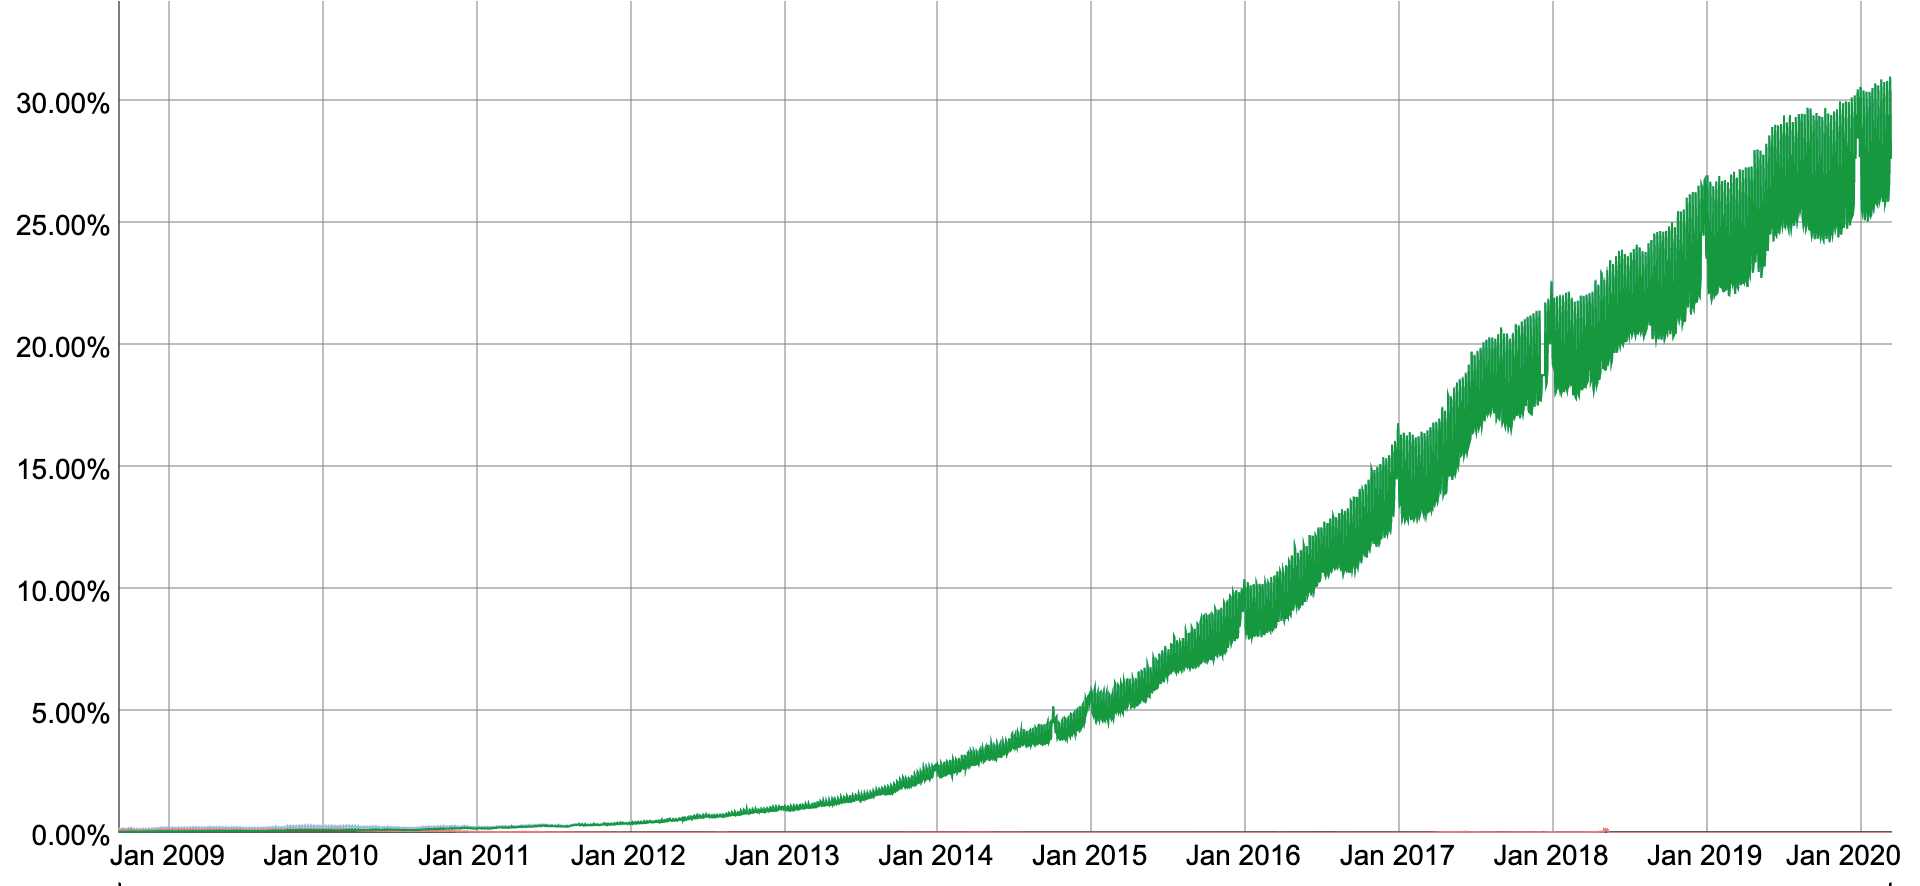
\includegraphics[width=0.9\textwidth]{IPv6_deploy_trend.png}
    \caption{IPv6部署率变化趋势}
    \label{fig:IPv6_deploy_trend}
  \end{figure}

  与此同时,由于互联网诞生之初的目标是成为美国内部学术机构和军事机构之间的连接设施,其假定了不存在恶意的参与者连接入网络,因而没有将网络的安全性作为最初设计时的主要目标之一。然而,随着互联网作为一项基础设施在全世界范围内得到广泛的应用,网络中恶意的攻击者层出不穷,网络体系结构设计中的安全问题也日益凸显。例如,分布式拒绝服务攻击(Distributed Denial of Service, DDoS)\cite{mirkovic2004taxonomy,douligeris2004ddos}至今仍在世界范围内广泛发生,每时每刻都在造成巨大的经济损失\cite{Kaspersky,DDosCost}。在美国白宫国家科技委员会网络和信息技术研发分委会发布的《网络安全研发战略规划》\cite{USStrategyPlan}中,网络安全的防御被分为四个主要阶段:威慑、保护、检测和适应,四者应对网络攻击时起效的顺序如图\ref{fig:security_methods}所示。可见,如果拥有强大的威慑手段,则很大一部分攻击者会因为攻击可能导致的后果而放弃发动攻击,而对于不惜代价发动的攻击行为,有效的保护手段则可以最大程度地减少攻击所带来的损失。
  \begin{figure}[ht]
    \centering
    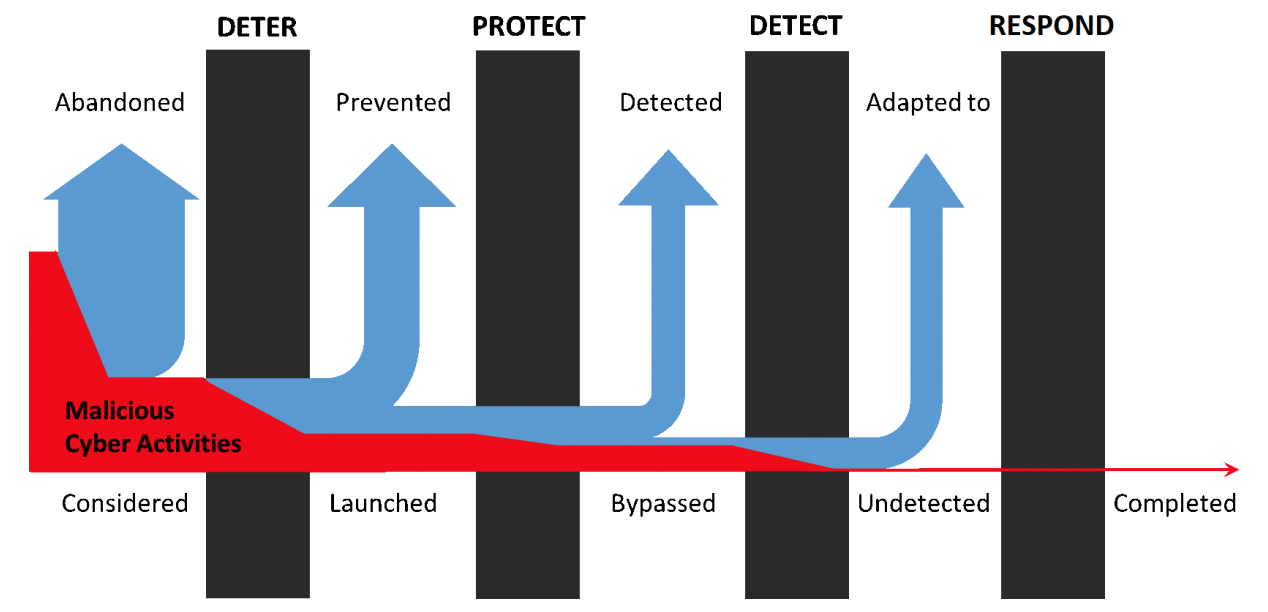
\includegraphics[width=0.9\textwidth]{security_methods.png}
    \caption{应对网络安全攻击的防御手段}
    \label{fig:security_methods}
  \end{figure}

  然而,现有的互联网体系结构并不能很好地对网络攻击实施有效保护,更难以谈及有力的威慑。主要原因在于现在的网络体系结构中,在转发网络数据包时,仅仅关注于根据目的IP地址进行数据包的转发,而不对数据包源IP地址的真实性进行检查。著名的STRIDE威胁模型\cite{kohnfelder1999threats}指出,网络安全问题层出不穷的根源在于源地址的伪造和难以溯源。缺乏对源IP地址真实性的验证机制使得伪造源IP地址的网络攻击流量在转发途中不受任何阻碍,即使能够在攻击对象的那一端对其进行阻止,也足以对网络带宽造成巨大的损耗,占用网络中转发其他正常流量的资源,从而影响网络整体的效益。此外,由于源IP地址不具备真实性的保证,同时IP地址又具有动态配置的特性,与现实世界中的用户实体不相关联,当网络攻击行为发生并被检测到时,人们仅能针对攻击流量进行一定程度的防御,而无法根据其源IP地址追溯到现实世界中的攻击者身份,令其为攻击行为所造成的危害负责,因而极大地损失了对攻击者的威慑力,导致威慑这第一步防御手段形同虚设。

  因此,现有的网络体系结构需要首先解决网络源IP地址伪造的问题,然后在源地址真实的前提下进行IP地址与用户身份的绑定、实现对用户真实身份的溯源功能,从而提供阻断攻击者恶意伪造流量的有效防御手段,并通过有力的审计和追责机制对攻击者形成强烈的威慑。

  针对IP源地址伪造的问题,源地址验证体系结构(Source Address Validation Architecture, SAVA)\cite{RFC5210}提出将互联网划分为接入子网、自治域内和自治域间三个层次,在每个层次分别研究相应的真实源地址验证技术,为源地址伪造的问题提供体系化的解决方案。源地址验证技术的研究,将从体系结构的角度提高网络空间整体的可信性,从根源上杜绝网络空间安全问题的发生,避免网络安全传统研究思路的补丁式解决方案。

  在源地址真实的基础上,充分利用IPv6地址空间巨大的优势,结合用户访问网络时的身份认证手段,通过将网络空间中的IPv6地址与现实世界中的用户身份相绑定的方式,设计实现并推广部署用户身份识别与溯源系统,将解决恶意网络行为责任人的溯源问题,提高对网络行为的精细化管控能力。

  在用户身份识别与溯源系统推广至多个管理域进行大规模部署时,还将面临跨管理域的用户身份溯源问题。由于涉及到用户隐私,因此用户身份溯源的权限必须谨慎地集中控制,而集中式的系统设计又难以抵御数据篡改与拒绝服务攻击,并且引入额外的信任成本。在消除集中式的可信第三方、提升系统可用性与提供数据保护方面,一种叫做区块链(Blockchain)的技术提供了新的解决方案,在近年来引发了人们的广泛关注。其最初作为底层的数据存储技术诞生于比特币(Bitcoin)\cite{nakamoto2019bitcoin}这一虚拟货币之中,但随即由于其去中心化和不可篡改的特性引发了人们的关注,在解决各个行业的一些传统痛点问题方面被寄予厚望。针对比特币协议合约脚本难以扩展的问题而提出的以太坊\cite{wood2014ethereum}与超级账本技术\cite{dhillon2017hyperledger},提供了执行用户自定义合约的能力,使得区块链在实现许多传统软件应用功能的同时,又提供了状态的多副本备份和不可篡改的特性,能够有效提升系统的可用性和安全性,因此吸引了大量的开发者利用区块链构建自己的分布式应用,并被广泛尝试应用于加密货币、金融资产结算、数字政务、防伪存证、物流溯源等多个交叉领域,形成了繁荣的生态。

  \section{论文研究工作与意义}
  \label{introduction:work}
  在传统的网络用户接入场景中,为了对用户上网行为实施精细化管控,并提供一定程度的用户身份审计功能,网络管理者往往通过在网络中实施接入认证的方式获取用户身份,并将用户身份与分配给该用户的IP地址形成绑定关系存在数据库中。但是,在网络中缺乏对源地址保护的情况下,即使进行了IP地址与用户身份的绑定,恶意用户仍可以轻易地伪造IP地址进行网络访问,从而逃避溯源与追责,甚至将恶意行为责任转嫁给其他用户。

  因此,基于IPv6源地址验证技术,在保证地址真实的基础上,研究用户身份识别与溯源技术,更具有现实意义。其与SAVA的源地址验证体系结构关系如图\ref{fig:SAVA_architecture}所示:
  \begin{figure}[ht]
    \centering
    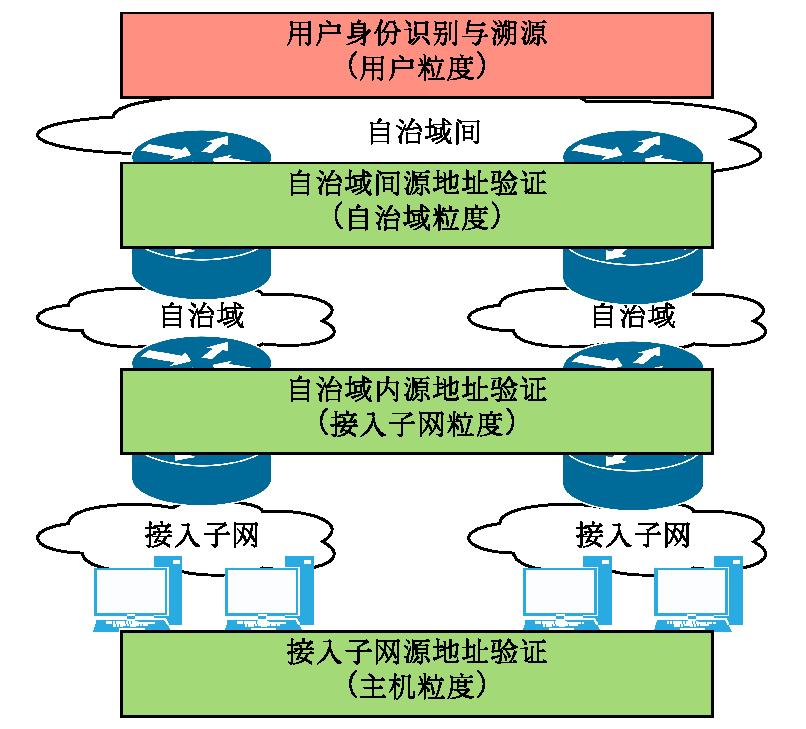
\includegraphics[width=0.7\textwidth]{SAVA_architecture.pdf}
    \caption{用户身份识别与溯源技术研究体系结构}
    \label{fig:SAVA_architecture}
  \end{figure}

  \begin{itemize}
    \item \textbf{接入子网源地址验证}:主机粒度的伪造源地址报文过滤是实现用户身份识别与溯源技术的前提,只有在接入子网内任意用户均只能使用自己真实的IPv6地址访问网络的情况下,最上层基于IPv6地址进行用户身份溯源的技术才不会发生失效或错误溯源的问题。目前接入子网源地址验证的SAVI技术\cite{RFC6959,RFC7039,RFC6620,RFC7513,RFC7219,I-D.bi-savi-wlan}已在IETF基本全部完成标准化,华为、新华三等设备厂商也对其进行了实现与支持,但要实现接入子网内完全的地址防伪造能力,必须在第一跳接入交换机或AP处进行SAVI的全部署,这对于使用目前尚未支持SAVI技术的厂商设备或老旧版本设备的大量接入子网而言,可能存在高昂的替换升级成本,为在接入子网内实现完全的源地址真实造成了一定阻力。
    \item \textbf{自治域内源地址验证}:在自治域内这一层次,由于域内各接入子网的网络均处于同一个管理域的管辖之下,在组网时网络管理员也可以容易地对各接入子网的IP前缀配置过滤规则,因此域内的源地址伪造问题相对而言并不严重,也容易通过一些配置手段加以解决。
    \item \textbf{自治域间源地址验证}:在自治域间发生的源地址伪造,可能导致合法用户遭到恶意用户的跨域伪造,使得用户身份识别与溯源发生错误。由于各自治域有着各自不同的利益考量,部署对自身出域报文的源地址进行验证的技术往往徒增运维负担,而难以带来收益,因此自治域间常需要结成互相信任的安全联盟以进行协作,增加域间源地址验证技术的部署收益。但加入安全联盟的自治域需要依赖于一个可信第三方维护自治域间的互信关系、记录各自治域控制平面通信所需信息,一旦该依赖遭到攻击导致服务不可用或数据篡改,将影响所有自治域间报文的转发,存在着严重的安全隐患。
  \end{itemize}


  即使在源地址得到真实性验证的前提下,传统网络管理中IP地址与身份绑定以实现用户身份溯源这种方式仍存在以下问题:
  \begin{itemize}
    \item \textbf{绑定关系错误}:IP地址的时分复用以及采用NAT技术将多个用户映射至同一个IP地址的不同端口易导致IP地址绑定到错误用户的情况,同时追溯用户时需要确定分组的时间信息,为身份溯源带来困难。
    \item \textbf{存储开销巨大}:为了实现对过去时刻的用户身份追溯,必须将历史上用户接入后的所有绑定关系均保存下来,这在用户时常切换、IP地址分配关系时常变更的网络中常常是难以承受的存储开销。
    \item \textbf{追溯过程复杂}:在互联网中存在数以万计的管理域,对网络攻击行为进行审计的实体与管理该网络攻击行为来源地网络的实体往往来自不同的管理域,多管理域中用户溯源技术不统一以及管理域间的线下协同工作容易引发追溯审计的困难。
    \item \textbf{认证手段限定}:目前广泛实施的IP地址与用户身份绑定都要求在Web Portal认证的方式下进行,其限定了用户认证方式,在无线网络中对终端漫游的支持较差,并且不具备良好的推广性,难以支持二层准入认证的网络环境。
  \end{itemize}

  NIDTGA(Network Identity and Timestamp Generation Address)地址生成方案\cite{liu2015building}针对上述问题,设计了一种通用的用户网络身份标识(Network Identity,NID),并利用IPv6广大地址空间的优势,采取了将NID与用户接入时间进行对称加密后嵌入IPv6的方式为用户生成和分配一种特定的IPv6地址,从而在保护用户隐私的同时将用户身份与IPv6地址实现了强绑定。由于NID结构的通用性,NIDTGA地址生成方案可以适用于用户数量不同的各类管理域。NIDTGA地址加密生成的方式,保证了审计方只需要持有用于生成地址时对称加密的密钥,即可追溯获得标识了用户身份的NID以及用户接入网络的时间,避免了巨大的用户信息绑定的存储开销和复杂的追溯过程。同时,由于嵌入了用户认证上网的时间信息并采用加密方式生成地址,基本消除了IPv6地址的混用情况,用户身份与IPv6地址的绑定错误也被良好避免。

  但是,尽管NIDTGA地址生成方案在理论上解决了传统网络中用户上网行为管理和审计的困难,但其仅给出了NID与NIDTGA地址的设计与生成方法,将用户的上网过程理想化为先提交NID完成认证、后获取NIDTGA地址这样两个简单的步骤,采用其生成算法的用户身份识别与溯源系统仍需要根据实际网络环境进行具体的设计。事实上,用户身份的获取是网络中认证系统的功能,IPv6地址配置是用户设备与相关的IPv6地址配置系统的功能,NIDTGA地址生成方案由于将用户身份与IPv6地址相关联,要求认证系统与IPv6地址配置系统之间实现信息同步的机制,而实际的接入子网环境错综复杂,不仅有着各异的组网方式,还存在着多种广泛应用的认证系统与IPv6地址配置系统,任意一个因素的变化都将影响到用户身份识别与溯源系统的设计:
  \begin{itemize}
    \item \textbf{地址配置方式}:IPv6地址引入了无状态地址自动配置SLAAC协议,其由用户设备自行生成地址而非向一个集中式的服务器进行请求,不存在类似于DHCPv6服务器这样能够控制用户设备配置某个特定IPv6地址的集中控制点,SLAAC与DHCPv6这两者的差异将直接导致各自地址配置方式下用户身份识别与溯源系统的不同设计方案。
    \item \textbf{用户认证手段}:实际网络中得到广泛应用的认证手段多种多样。以网络层为界,常用于在链路层认证的有802.1X\cite{ieee802ieee}、PPPoE\cite{RFC2516}等协议,基于网络层往上进行用户认证控制的则有Web Portal认证、IPoE与Web Portal的组合认证等方式。是否基于网络层协议进行用户身份认证决定了IPv6地址配置过程发生在用户认证前还是认证之后,因此用户身份识别与溯源系统需要根据网络中具体的认证手段对其NIDTGA地址配置流程做出相应的设计。
    \item \textbf{设备类型}:不同厂商的设备对于地址配置方式的支持情况不同,使用Android、Chrome OS等Google系操作系统的用户设备目前不支持DHCPv6配置地址。此外,网络中不止包含普通的笔记本或手机终端,还包括服务器、嵌入式设备等难以进行身份认证的设备。设备类型的繁杂为用户身份识别与溯源系统实现设备全覆盖带来了挑战。
    \item \textbf{子网组网方式}:接入子网根据用户接入方式的不同,可分为有线子网与无线子网,两者对源地址验证技术的部署要求不同,源地址验证设备位置、子网网关位置、以及DHCPv6配置时DHCPv6中继设备位置也不相同。在无线子网配置时,若数据报文直接经由上层有线网络转发,则称为本地转发模式,若全部经由IP隧道到达AC后统一转发,则称为集中转发模式,两种转发模式下数据报文转发路径的不同将影响接入子网中网络设备的配置,同样也影响到用户身份识别与溯源系统的部署方案。
  \end{itemize}

  可见,用户设备如何在获取地址前进行身份认证、如何标识用户设备并将NIDTGA地址与其准确关联、如何在实际的复杂网络环境中进行部署等均是用户身份识别与溯源系统在设计与实现时需要考虑的重要问题。用户身份识别与溯源技术在利用NIDTGA的地址生成理论后,面向实际网络进行系统设计、实现与部署落地等方面还面临着巨大的挑战。

  本文根据上述分析,主要在三个方面开展研究工作:
  \begin{enumerate}[1{)}]
    \item \textbf{接入子网与自治域间源地址验证技术的增强方案。}

    SAVI技术在接入子网范围内进行源地址伪造报文的过滤,其功能的正确行使依赖于网络中各台设备对SAVI的支持与配置情况,其作为较新的国际标准尚未被所有厂商设备良好支持,如何在非理想的SAVI部署网络中进行接入子网源地址伪造的预防有待研究。另一方面,一类重要的自治域间源地址验证技术在方案设计上存在着共同的安全缺陷,其引入的安全联盟概念虽在一定程度上增加了方案的部署激励,但也为域间源地址验证系统的运作带来了单一故障点的安全风险。本文针对上述问题,分别研究采用传统网络设备普遍支持的其他机制配合SAVI技术以较小的代价实现接入子网源地址验证,以及利用区块链构建域间源地址验证方案中的安全联盟,在接入子网为用户身份识别与溯源系统的部署提供有力的源地址真实性保证,并为自治域间保障源地址真实消除重大的安全隐患,为用户身份识别与溯源系统的设计、应用与推广奠定良好的技术基础。

    \item \textbf{各类网络场景下用户身份识别与溯源系统的设计与实现。}

    NIDTGA地址生成方案提出以来,将其应用至实际的用户身份识别与溯源系统仍有待研究。在设计采用NIDTGA地址生成方案的用户身份识别与溯源系统时,由于系统工作于网络层而非仅仅在于应用层,其难以独立于网络环境采用的底层协议而实现统一设计,多种IPv6地址的配置方式、各类用户身份认证手段、不同厂商品牌型号的用户设备均会对用户身份识别与溯源的过程产生影响,因此具备应用推广意义的用户身份识别与溯源技术必须实现对多场景全用户的适配,提出各类网络环境中的用户身份识别与溯源系统设计方案与部署方案。本文首先调研了IPv6地址配置方式,并分析了实际网络中常见的用户认证手段、用户设备对各类地址配置协议与认证手段的支持情况,以确认用户身份识别与溯源系统需要覆盖的网络场景。然后分别针对各种常见地址配置方式与用户身份认证手段的组合,研究系统的设计方案。最后本文还调研了全国主要高校的组网情况,以常见的校园网环境为例,讨论了对用户身份识别与溯源系统进行推广时的网络设备支持要求,总结抽象出部署方案的指导框架。

    \item \textbf{基于区块链的跨管理域用户身份溯源系统设计与实现。}

    在用户身份识别与溯源系统推广部署的过程中,需要解决跨管理域的用户身份溯源问题。由于溯源过程涉及用户身份隐私,因此用户溯源权限必须谨慎地进行集中控制。但如果采用集中式的组织密钥历史存储与用户身份溯源,则存在中心化的安全风险,易受到恶意攻击,引发服务不可用或数据篡改,从而导致用户隐私泄露与溯源功能失效。如何多副本备份组织密钥历史并对其实施有效的数据保护,但仍集中地控制用户身份溯源权限,避免用户隐私泄漏,是跨管理域的用户身份溯源系统亟待解决的问题。本文研究将区块链应用于构建用户身份溯源系统的设计方案,利用区块链分布式的优势保证各组织密钥历史的多副本备份,利用其数据不可篡改的特性保证密钥历史的真实性,并且使用椭圆曲线加密算法加密密钥历史,以确保在数据对各个区块链节点可见的情况下仍只有审计方有能力读取各组织的密钥历史明文。

  \end{enumerate}


  \section{论文贡献}
  \label{introduction:contribution}
  本文的主要贡献包括:
  \begin{enumerate}[1{)}]
    \item 针对接入子网与自治域间源地址验证技术面临的安全问题,提出了基于VLAN划分的SAVI技术部署增强方案与基于区块链的安全联盟增强方案RegChain,分别解决了非理想的SAVI部署网络环境中的接入子网源地址伪造问题、自治域间SMA方案的单一故障点问题,为用户身份识别与溯源系统奠定良好的源地址真实性保障基础。
    \item 针对网络中用户身份识别与溯源能力的缺乏,提出了采用NIDTGA地址生成方案的用户身份识别与溯源系统,并给出了在各类地址配置方式、用户认证手段组合下的系统设计,提供了覆盖复杂的接入网络全场景的完备解决方案,并对各方案的优缺点进行了评价对比,给出了适宜推广的基于二次准入认证的系统在校园网络中的部署方案。
    \item 对各类网络场景下的用户身份识别与溯源系统设计进行了实现、测试与部署,其中DHCPv6配置下基于二次准入认证的系统已在清华大学无线校园网络中得到部署并计划在全国主要高校进行推广,基于扩展DHCPv6协议认证的系统已在清华、北大等5所高校进行了部署实验,并通过了国家发改委288项目的验收。在SLAAC下的用户身份识别与溯源技术基础上,增加了对MAC地址伪造的检测与预防的溯源方案已由华为和新华三厂商进行实现,并开始在清华大学无线网络中进行大规模部署与应用。
    \item 针对用户身份识别与溯源系统推广部署时的跨管理域溯源问题,提出溯源系统的区块链设计方案NIDChain,在提供数据安全与服务高可用优势的同时,设计了相应的权限控制机制确保用户身份溯源权限高度集中,为用户身份识别与溯源系统的大规模部署奠定了基础。
  \end{enumerate}


  \section{论文组织结构}
  \label{introduction:structure}
  本文共分六章,各章节之间的逻辑关系如图\ref{fig:thesis_structure}所示,具体组织如下:
  
  第一章为论文引言,主要介绍IPv6源地址验证与用户身份识别与溯源技术的背景、研究工作与意义以及论文对用户身份识别与溯源相关技术的贡献。

  第二章为论文相关研究工作的综述,主要介绍了IPv6地址的几种配置协议、源地址验证各个层次的相关技术、IPv6地址生成方案、现有的用户身份识别与溯源方案以及区块链的相关研究。
  
  第三章为论文研究的第一部分,IPv6源地址验证技术的增强方案,从接入子网与自治域间两个层次分别介绍了基于VLAN划分的SAVI部署增强方案与基于区块链的安全联盟增强方案RegChain。

  第四章为论文研究的第二部分,用户身份识别与溯源系统的设计、实现与部署。首先分析了用户身份识别与溯源系统需要支持的复杂网络场景,然后针对DHCPv6、SLAAC与静态地址三种地址配置方式下基于Web Portal、二层准入认证等不同用户认证手段的系统设计方案进行研究与实现,介绍了目前各场景下用户身份识别与溯源系统的应用现状,分析了各种设计方案的优劣性,并给出了在校园网络中部署应用的指南。

  第五章为论文研究的第三部分,基于区块链的用户身份溯源系统研究。提出了利用区块链构建跨管理域的溯源系统设计方案NIDChain,探讨了在区块链上所有数据公开透明的情况下确保各组织密钥历史的私密性并赋予审计方唯一追溯权限的机制,详细介绍了智能合约中密钥历史更新等各个功能的设计,并基于以太坊进行了实现。

  第六章对全文的工作进行了总结,并展望了后续推进用户身份识别与溯源技术的研究方向。

  \begin{figure}[ht]
    \centering
    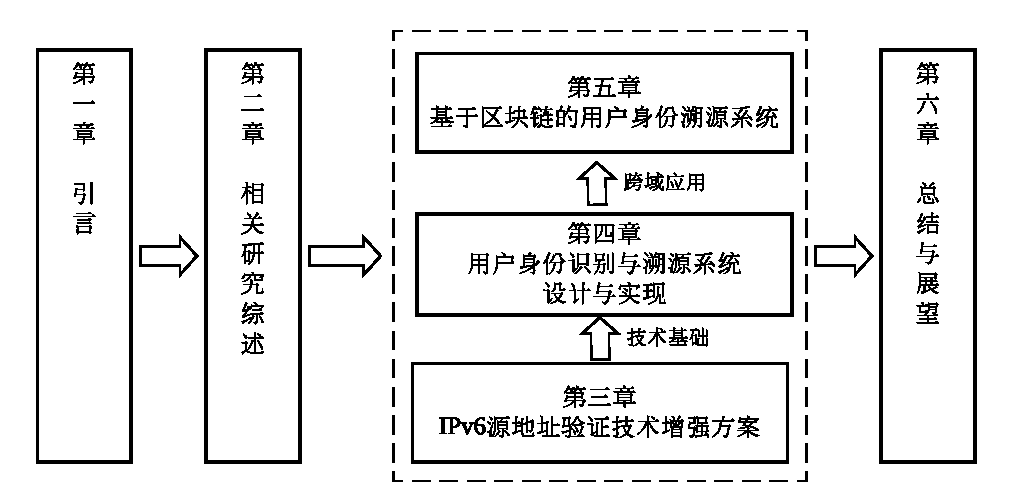
\includegraphics[width=0.9\textwidth]{thesis_structure.pdf}
    \caption{论文组织结构}
    \label{fig:thesis_structure}
  \end{figure}
% !TeX root = ../main.tex

\chapter{相关研究综述}
\label{survey}

  \section{本章引言}
  \label{survey:introduction}
  基于IPv6源地址验证的用户身份识别与溯源技术是采用NIDTGA地址生成方案将用户身份信息通过加密手段嵌入至IPv6地址的后64位接口标识中,实现根据IPv6地址溯源使用该地址的用户身份的技术。其以网络层IPv6地址的真实性作为前提,由用户身份标识生成、用户认证、NIDTGA地址的生成与配置、根据NIDTGA地址追溯用户身份、网络管理员更新地址生成密钥等多个环节共同组成。用户身份识别与溯源系统的实现需要衔接上述各个环节,其安全性涉及到用户认证信息安全、IPv6地址安全、生成NIDTGA地址的密钥历史安全等方面。
  
  为了实现基于IPv6源地址验证的用户身份识别与溯源系统,将其部署落地并在全国高校进行推广应用,本文对网络层IPv6地址配置方式进行调研,以确认用户身份识别与溯源系统需要支持的地址配置场景。
  源地址验证技术作为用户身份识别与溯源系统的基础,其良好部署与安全性保障也直接影响到用户身份识别与溯源系统的正常运作,因此本章从接入子网、自治域内与自治域间三个层次分别对源地址验证的相关研究进行讨论。
  由于IPv6地址引入了有别于IPv4的新的地址配置方式,因此存在多种IPv6地址生成方案的研究,本文对各方案的侧重点进行讨论,其中包含用户身份识别与溯源技术所采用的NIDTGA地址生成方案。同时,对当前网络环境中常实施的用户身份认证手段进行介绍,并分析了常见溯源方案所存在的问题。此外,由于本文研究利用区块链提升用户身份识别与溯源系统及其基础技术的安全性,因此也对区块链技术的原理与发展现状进行了综述,为区块链方案的设计与实现提供指引。

  本章内容组织如下:第\ref{survey:configuration}节综述了IPv6地址的各种配置方式;第\ref{survey:sava}节根据SAVA体系结构的划分讨论各层次的源地址验证相关技术;第\ref{survey:generation}节描述了现有的IPv6地址生成方案,重点介绍了NIDTGA地址的生成方法;第\ref{survey:identity}节对现有的用户身份认证手段与溯源方案进行讨论;第\ref{survey:blockchain}节描述了区块链技术的发展现状;第\ref{survey:summary}节对本章进行总结。

  \section{IPv6地址配置方式的研究}
  \label{survey:configuration}
  IPv6地址的配置方式有三种,分别为:IPv6动态主机配置协议(Dynamic Host Configuration Protocol for IPv6,DHCPv6)\cite{RFC8415}、IPv6无状态地址自动配置(IPv6 Stateless Address Autoconfiguration,SLAAC)\cite{RFC2462}与IPv6静态配置。

  用户设备在接入网络时,根据接入子网网关设备周期性发送的路由器公告(Router Advertisement,RA)报文\cite{RFC2461,RFC5175}中的标志位来判断采用何种地址配置方式。RA报文中的Managed标志位与Other标志位被用于向用户设备告知子网的控制报文可达链路中存在可提供IPv6地址配置的DHCPv6服务器。RA报文中的Autonomous标志位则用于表示用户设备可采用SLAAC方式自动生成RA所公告IPv6前缀下的IPv6地址。

    \subsection{动态主机配置}
    \label{survey:configuration:DHCPv6}
    DHCPv6协议\cite{RFC8415}中定义了DHCPv6地址配置过程中涉及到的三种实体类型,DHCPv6客户端、DHCPv6中继与DHCPv6服务器。DHCPv6客户端一般由用户设备的操作系统内核提供;DHCPv6中继则由网络中的交换机或路由器等设备开启相应功能,负责将DHCPv6报文在不同链路之间进行中继转发;DHCPv6服务器负责集中管理其可提供的IPv6地址资源,响应用户设备的地址请求,根据自身策略选择可用的IPv6地址提供给用户,并设置租约时长等信息。由于DHCPv6服务器负责维护已配置的IPv6地址状态,因此若用户需要继续使用IPv6地址,则设备需要在DHCPv6服务器设置的租约时间到期前,向DHCPv6服务器发送续约报文以进行IPv6地址租约时间延长的请求。一个典型的DHCPv6地址配置流程如图\ref{fig:dhcpv6_no_relay}所示:
    \begin{enumerate}[1{)}]
      \item 首先,用户设备以组播地址FF02::1:2为目的地址,以自身的本地链路地址为源地址,发送Solicit报文,寻找可达链路中的DHCPv6服务器。
      \item DHCPv6服务器将在传输层547号端口监听用户设备或DHCPv6中继发送的DHCPv6报文,当收到Solicit报文时,其将根据自身的地址池状态与用户所在链路情况判断是否为请求的设备提供IPv6地址,若是,则向设备回复Advertise报文,其中包含DHCPv6服务器选择提供的IPv6地址、租约时间等信息。
      \item 用户设备收到若干个DHCPv6服务器回复的Advertise报文时,其将根据DHCPv6客户端的自身策略从其中选择一个IPv6地址,向其对应DHCPv6服务器发送Request报文,请求正式配置地址。
      \item 在收到Request报文后,若原先提供的IPv6地址仍有效,则DHCPv6服务器向用户设备回复一个Reply报文,其中包含此前Advertise报文所指定的各项信息;
      \item 用户设备收到最终的Reply报文后,根据其中包含的信息配置其网络适配器的IPv6地址,接入网络。
      \item 当IPv6地址租约中指定的T1时间到期时,用户设备将发送Renew报文,请求拓展IPv6地址租约时间。
      \item 在收到Renew报文后,若DHCPv6服务器检查状态后允许续约,则向设备回复Reply报文,指定新的租约时间,并更新自己维护的IPv6地址池状态。
    \end{enumerate}

    \begin{figure}[ht]
      \centering
      \subcaptionbox{无中继DHCPv6地址配置\label{fig:dhcpv6_no_relay}}
      {\includegraphics[height=5cm]{dhcpv6_no_relay.pdf}}
      \hspace{2em}
      \subcaptionbox{有中继DHCPv6地址配置\label{fig:dhcpv6_with_relay}}
      {\includegraphics[height=5cm]{dhcpv6_with_relay.pdf}}
      \caption{DHCPv6地址配置与续约流程}
      \label{fig:dhcpv6_configure}
    \end{figure}

    在实际的网络环境中,由于一个管理域中往往包含数量庞大的网络链路,为了管理的便利,通常只部署二到三台DHCPv6服务器,而不是在每一个链路中均进行部署,因此DHCPv6协议还支持如图\ref{fig:dhcpv6_with_relay}所示的中继机制:
    
    \begin{itemize}
      \item 对于Solicit、Request、Renew等由DHCPv6客户端发出的报文,DHCPv6中继将其作为Relay Forward报文中的中继报文选项Option 9所携带的值,并根据DHCPv6中继的配置设置其他一些选项,如设备的源MAC地址等,然后将Relay Forward报文组播发送到其他链路中;
      \item 对于Advertise、Reply等由DHCPv6服务器发出的报文,DHCPv6中继将其作为Relay Reply报文中的中继报文选项Option 9所携带的值,并根据配置设置其他的选项,然后将Relay Reply报文发送到对应链路中。
    \end{itemize}

    DHCPv6报文通过IETF标准定义的选项携带DHCPv6配置时的相关信息,较为重要的有DHCPv6唯一标识符DUID(DHCPv6客户端为Option 1,DHCPv6服务器为Option 2)、非临时IPv6地址与租约时间(Option 3)等信息。DHCPv6中继也可在封装后的中继报文中添加选项,比如Subscriber-ID选项(Option 38)\cite{RFC4580}携带在网络发生变化时保持不变的设备独立标识、Client Link-Layer Address选项(Option 79)\cite{RFC6939}携带用户设备的链路层地址等。

    由于DHCPv6协议采取集中式的地址管理方式,管理者可根据需要自主选择为用户设备分配的IPv6地址,并且其有状态的地址配置有利于管理者对用户设备上网行为进行管理,方便地址资源的管理和策略定制。

    \subsection{无状态地址自动配置}
    \label{survey:configuration:SLAAC}
    SLAAC协议\cite{RFC2462}与DHCPv6协议不同,没有一个集中式的服务器控制IPv6地址资源的分配,而是通过RA报文宣告IPv6地址前缀与SLAAC地址配置方式,告知用户设备使用相应的IPv6地址前缀生成IPv6地址进行配置。一个典型的SLAAC地址配置场景如图\ref{fig:slaac_configure}所示:
    \begin{enumerate}[1{)}]
      \item 网关设备向用户设备发送路由器公告RA报文,置位Autonomous标识位,包含可配置的IPv6前缀等信息。
      \item 用户设备根据自身选择的IPv6地址生成算法,一般采用EUI-64,生成IPv6地址的后64位接口标识,与RA报文中的IPv6前缀进行拼接,形成IPv6单播地址作为设备的试验地址。
      \item 用户设备在生成试验地址后将随机延迟一段时间,构建邻居请求(Neighbor Solicitation,NS)报文,以试验地址作为NS报文探测的目标地址,将其向试验地址所述的Solicited-Node组播地址发送以进行重复地址检测。
      \item 同一Solicited-Node组播组的其他节点收到NS报文后,检查其中目标地址是否与自身配置或正在试验配置的IPv6地址相冲突;若与自身已配置的地址相冲突,则向源设备回复宣告已持有该IPv6地址的邻居公告(Neighbor Advertisement,NA)报文;若与自身正在试验配置的IPv6试验地址冲突,则进行退让处理,不发送NA报文,重新生成IPv6地址进行试验配置。
      \item 若用户设备在等待时间内未收到其他节点发来的、以相同IPv6地址为目标地址的NS报文或NA报文,则重复地址检测成功,设备为其网络接口配置该IPv6地址,并设定网关地址等信息。
    \end{enumerate}

    \begin{figure}[ht]
      \centering
      \includegraphics[width=0.9\textwidth]{slaac_configure.pdf}
      \caption{SLAAC地址配置与重复地址检测流程}
      \label{fig:slaac_configure}
    \end{figure}

    SLAAC方式地址配置流程简单,不需要DHCPv6服务器的介入,但这种简单性导致了用户所使用的IPv6地址不受网络管理者的控制,因此难以对用户设备的地址选择策略进行定制和精细化控制,一些复杂的主机配置信息也难以通过这种方式进行传递。

    \subsection{静态配置}
    \label{survey:configuration:manual}
    IPv6静态配置方式通过人工向配置文件中写入IPv6地址、子网网关地址、DNS服务器地址等信息完成对用户设备的配置。静态配置的方式由配置人员在线下向网络管理员确定网络的配置信息,因此网络管理者也可以对其地址分配策略进行定制,实现较为精细的管理,但同时也需要对向用户设备提供接入功能的网络设备进行相应的配置以避免用户伪造、滥用IPv6地址。静态配置的方式容易出现错误,也不适合大规模的网络设备配置场景。
  
  \section{源地址验证的相关研究}
  \label{survey:sava}

    \subsection{接入子网源地址验证}
    \label{survey:sava:access}
    在SAVA\cite{RFC5210}的体系结构中,接入子网的源地址验证技术处于最靠近用户设备的位置,因而能够实现最为精细的源地址伪造报文的过滤。为了实现用户身份识别与溯源技术的IPv6真实性前提,其需要提供主机粒度的源地址验证,保证处于子网内的用户设备不能使用其他任何非自身配置的IPv6地址作为报文的源地址访问网络。SAVI技术\cite{RFC7039,RFC6959,RFC6620,RFC7513,RFC7219,I-D.bi-savi-wlan}通过对地址配置过程中控制报文的监听,在设备接入点建立相应的过滤表项,将用户配置的IP地址与网络中标识了该用户接入且不可伪造的绑定锚相绑定,在用户发送数据报文访问网络时对其报文源地址与绑定锚的匹配关系进行校验,以实现对伪造源地址报文的过滤。目前,SAVI技术已被IETF标准化,专为无线网络设计的SAVI技术\cite{I-D.bi-savi-wlan}也已成为SAVI草案,处于国际标准化流程中,SAVI已成为接入子网源地址验证技术的标准。
    在众多SAVI技术相关的标准中,RFC 6959\cite{RFC6959}与RFC 7039\cite{RFC7039}作为基础性标准,分别对SAVI体系中涉及的各类对象和SAVI框架进行了定义和描述。在此之上,SAVI针对DHCPv6、静态配置与SLAAC以及无线网络中的SAVI的实现均进行了具体设计。

      \subsubsection{SAVI的绑定锚}
      \label{survey:sava:access:anchor}
      在SAVI的设计中,绑定锚是一个至关重要的概念,其代表了网络中SAVI可以信任的不会发生伪造的对象,同时必须与接入的用户设备相关联以实现与用户合法IP地址的一一绑定。交换机端口、不可更改的用户设备MAC地址或其他用户难以伪造的信息均可以作为绑定锚\cite{RFC6959}。在有线网络中,选择部署SAVI的交换机的端口作为绑定锚,因此一般需要在第一跳接入交换机处即启用SAVI以防止同一端口下的不同设备间发生IP地址伪造;在启用了802.1X认证的情况下,也可以选择MAC地址作为绑定锚\cite{RFC6959}。在无线网络中,由于不具备实体的链路,因此不存在不可伪造的端口实体,需要通过802.11i\cite{IEEE80211i}等机制保证用户设备的MAC地址安全,以设备MAC地址作为SAVI的绑定锚。

      \subsubsection{SAVI的绑定表项建立}
      \label{survey:sava:access:listen}
      SAVI绑定表项通过监听网络中的控制报文交互流程进行建立。
      
      在DHCPv6配置地址的情况下,其监听DHCPv6协议的标准交互流程,在DHCPv6服务器答复Reply报文成功为用户设备配置IPv6地址时,SAVI交换机或AP将该IPv6地址与交换机端口或用户设备MAC地址进行绑定\cite{RFC7513}。在静态配置或SLAAC配置地址的情况下,用户设备配置了静态地址或SLAAC试验地址后,将组播发送NS报文进行重复地址检测,SAVI设备监听这个重复地址检测的过程,若不发生冲突则将目标地址与绑定锚进行绑定\cite{RFC7219,RFC6620},否则SAVI设备将向原先持有目标IPv6地址的设备再次发送NS报文以进行二次确认,若能够确认应答则不发生表项迁移,否则将目标IPv6地址迁移为与新的绑定锚进行绑定的SAVI表项。

      在有线网络中,选择SAVI交换机端口为绑定锚,SAVI绑定表项包含内容一般有:IP地址、VLAN号、MAC地址、端口、老化时间等。以前两者为索引,不可重复,在对报文进行检查时匹配前四项的一致性。在无线网络中,由AC配置AP启用SAVI,AP对用户设备地址配置过程进行监听,建立以MAC为索引的MAC地址、IP地址绑定项,并上传至AC生成包含IP地址、MAC地址、AP信息、老化时间等内容的绑定表项,当用户发送数据报文时,由AP对其进行源地址检查与过滤,当用户发生漫游时,AC将用户表项下发给对应的新AP以进行SAVI表项迁移。

      \subsubsection{SAVI的安全边界与扩展性}
      \label{survey:sava:access:bound}
      部署SAVI的子网需要形成一个安全边界,即所有数据报文在三层转发前必须经过至少一个SAVI设备,以保证子网内不会发生跨越安全边界的源地址伪造。如图\ref{fig:SAVI_bound}所示,左侧子网1以汇聚交换机为网关,其下的接入交换机均部署了SAVI,此时子网1中所有设备的报文在转发时均需要经过至少一台SAVI设备,子网1的所有接入交换机构成了子网1的安全边界。右侧子网2的网关在核心设备上,其接入交换机并不全部支持SAVI,但上连核心路由器的汇聚交换机支持SAVI,此时支持SAVI的接入层交换机与汇聚交换机构成了子网2的安全边界。SAVI技术保证了在构成安全边界的前提下,接入子网内不会发生跨越安全边界的伪造,比如子网1内设备A、B不能互相伪造源地址,子网2内设备A不能伪造设备B、C的地址,设备B、C也不能伪造设备A的源地址。但是对于未到达SAVI安全边界时内部发生的源地址伪造,SAVI无法进行识别,比如在子网2内部,由于设备B和C均被其汇聚交换机绑定在同一物理端口,设备B和C之间互相进行MAC地址与源IP地址的同时伪造对SAVI而言难以预防,因此推荐在SAVI部署时必须部署在第一跳接入交换机。在无线场景下,则必须令AP均开启SAVI功能,对伪造源地址的报文进行过滤。
      \begin{figure}[ht]
        \centering
        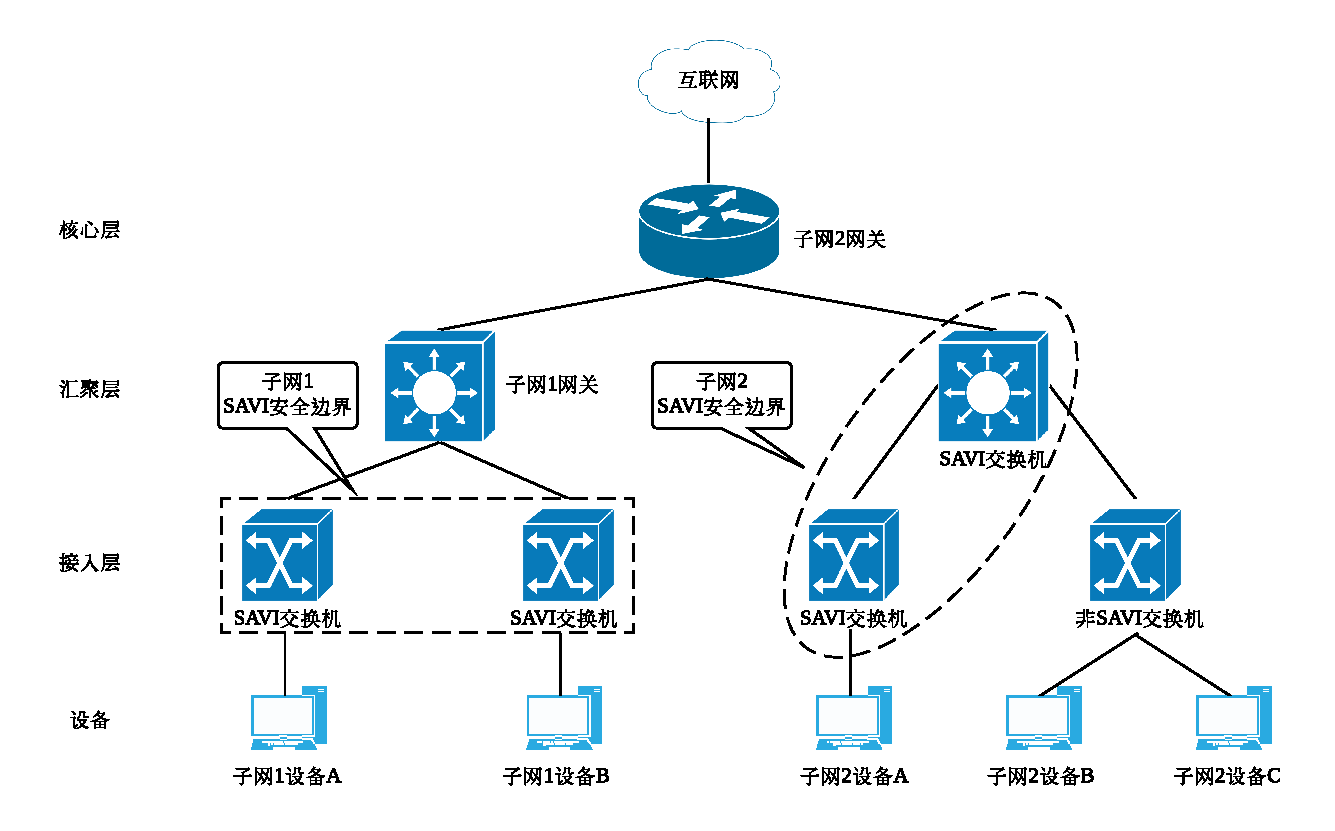
\includegraphics[width=0.9\textwidth]{SAVI_bound.pdf}
        \caption{SAVI安全边界示意}
        \label{fig:SAVI_bound}
      \end{figure}

      此外,在图\ref{fig:SAVI_bound}中,子网2内支持SAVI的接入交换机与汇聚交换机形成了级联的关系,在接入交换机已经对报文进行过滤的情况下,汇聚交换机不必再次进行SAVI绑定表的建立与报文的检查,因此为了在多SAVI交换机级联的场景下避免表项冗余,SAVI技术支持设置SAVI Trust端口,对其下的报文进行信任,不进行控制报文监听和数据报文过滤,从而支持网络的大规模扩展。

    \subsection{自治域内源地址验证}
    \label{survey:sava:intraas}
    自治域内的源地址验证技术需要进行IP地址前缀粒度的伪造报文过滤,避免同一自治域内某一子网的用户使用不属于其所在子网的IP地址向外发送报文的情况发生,其伪造报文过滤粒度在子网级别。目前域内源地址验证技术的研究相对较少,这一方面是由于自治域一般属于同一个管理域,所有接入子网都处于网络管理员的管辖之下,域内源地址伪造的问题不易发生,另一方面也由于可以通过在接入子网网关设备处进行一些简单的配置以进行域内伪造报文的过滤,自治域内源地址验证方案的部署收益不高。

    通过ACL(Access Control List)的手段可在各子网网关处配置对报文源地址进行检查,仅允许使用来自本子网地址作为源IP的报文通过,从而实现不同子网之间的设备不发生源地址伪造。
    uRPF(unicast Reverse Path Forwarding)\cite{uRPF}使用转发表作为过滤表,避免了ACL的手动配置,但其仅适用于对称路由的域内结构,对于需要增强网络可用性而常具有链路备份的组网方式而言容易发生错误丢弃正确报文的假阳性问题。
    SAVO\cite{I-D.tao-savi-savo}基于OSPF协议\cite{RFC2740}学习域内的链路状态并计算合法的报文转发路径,以消除uRPF对对称路由的假设。但自治域内往往不止OSPF一种路由协议,还可能存在手动配置的静态路由,基于OSPF难以获得完整的路由拓扑信息,也可能出现假阳性等问题。
    CPF(Calculated Path Forwarding)\cite{duan2006constructing}通过SNMP\cite{RFC3411,RFC3413}从域内的路由器中收集管理信息数据MIB,从而获取域内的路由信息,并计算域内报文转发的合法路径,生成伪造报文的过滤规则,并通过SSH\cite{RFC4251}配置到各路由器的ACL中,从而减轻手工配置的负担,并消除假阳性等问题。

    \subsection{自治域间源地址验证}
    \label{survey:sava:interas}
    自治域间源地址验证技术是解决跨域源地址伪造问题的验证技术。由于其研究对象涉及多个自治域,自治域间利益难以统一,单一自治域部署源地址验证技术只会增加自治域管理员的运维负担,却没有提供防御来自其他自治域的恶意流量的能力,因而自治域间源地址验证的方案往往缺乏部署激励。根据自治域间源地址验证技术原理的不同,本文将其划分为基于端到端验证思想的方案与基于拓扑验证思想的方案两类。

      \subsubsection{端到端验证类自治域间源地址验证方案}
      \label{survey:sava:interas:tag}
      端到端验证类方案是指基于如下思路的一类技术:通信的自治域双方首先建立相互的信任关系,在发送域间报文前首先在控制平面协商验证域间报文源地址真实性的方法,源自治域的数据平面为出域报文添加根据协商方法生成的保障报文源地址真实性的标签,由目的自治域数据平面根据控制平面传递的信息验证入域报文所携带标签的合法性从而判断源地址的真伪,如图\ref{fig:end_to_end_validation}所示。

      \begin{figure}[ht]
        \centering
        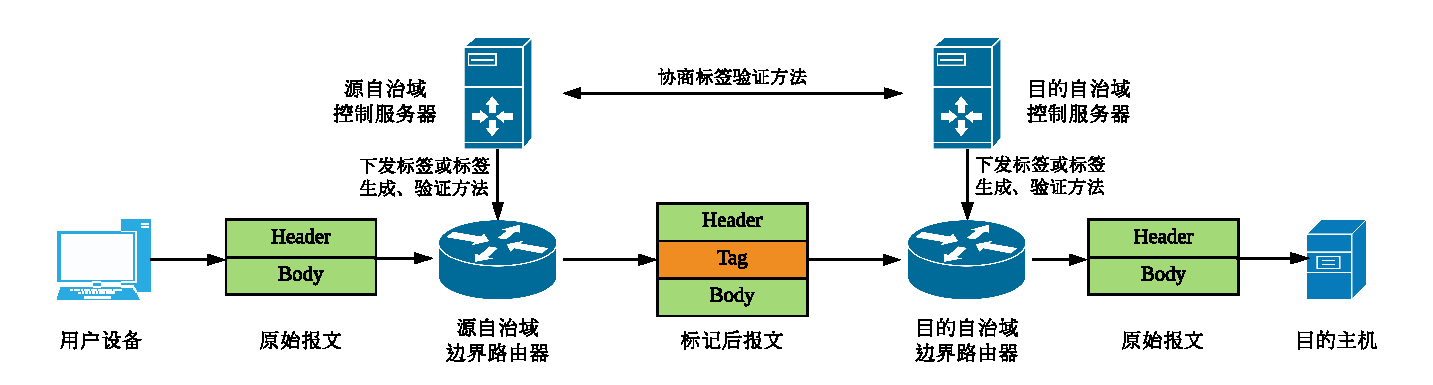
\includegraphics[width=0.9\textwidth]{end_to_end_validation.pdf}
        \caption{端到端验证类自治域间源地址验证方案原理}
        \label{fig:end_to_end_validation}
      \end{figure}

      为实现自治域间端到端的标签验证,自治域的控制平面需要首先建立通信确认对方可信的身份,因而各类方案均不可避免地引入一个安全联盟的概念以确保对方自治域的行为受到一定的约束,同时采用可信的第三方维护自治域控制平面的信息,以使各自治域控制平面之间能够顺利建立通信并确认身份。因此,基于端到端验证思想的自治域间源地址方案拓扑一般如图\ref{fig:end_to_end_validation_topology}所示。可见,维护自治域之间互信关系的可信第三方在端到端验证方案中具有特殊地位,其工作正常与否将直接影响到所有部署了自治域间源地址验证方案的自治域间报文的转发。

      \begin{figure}[ht]
        \centering
        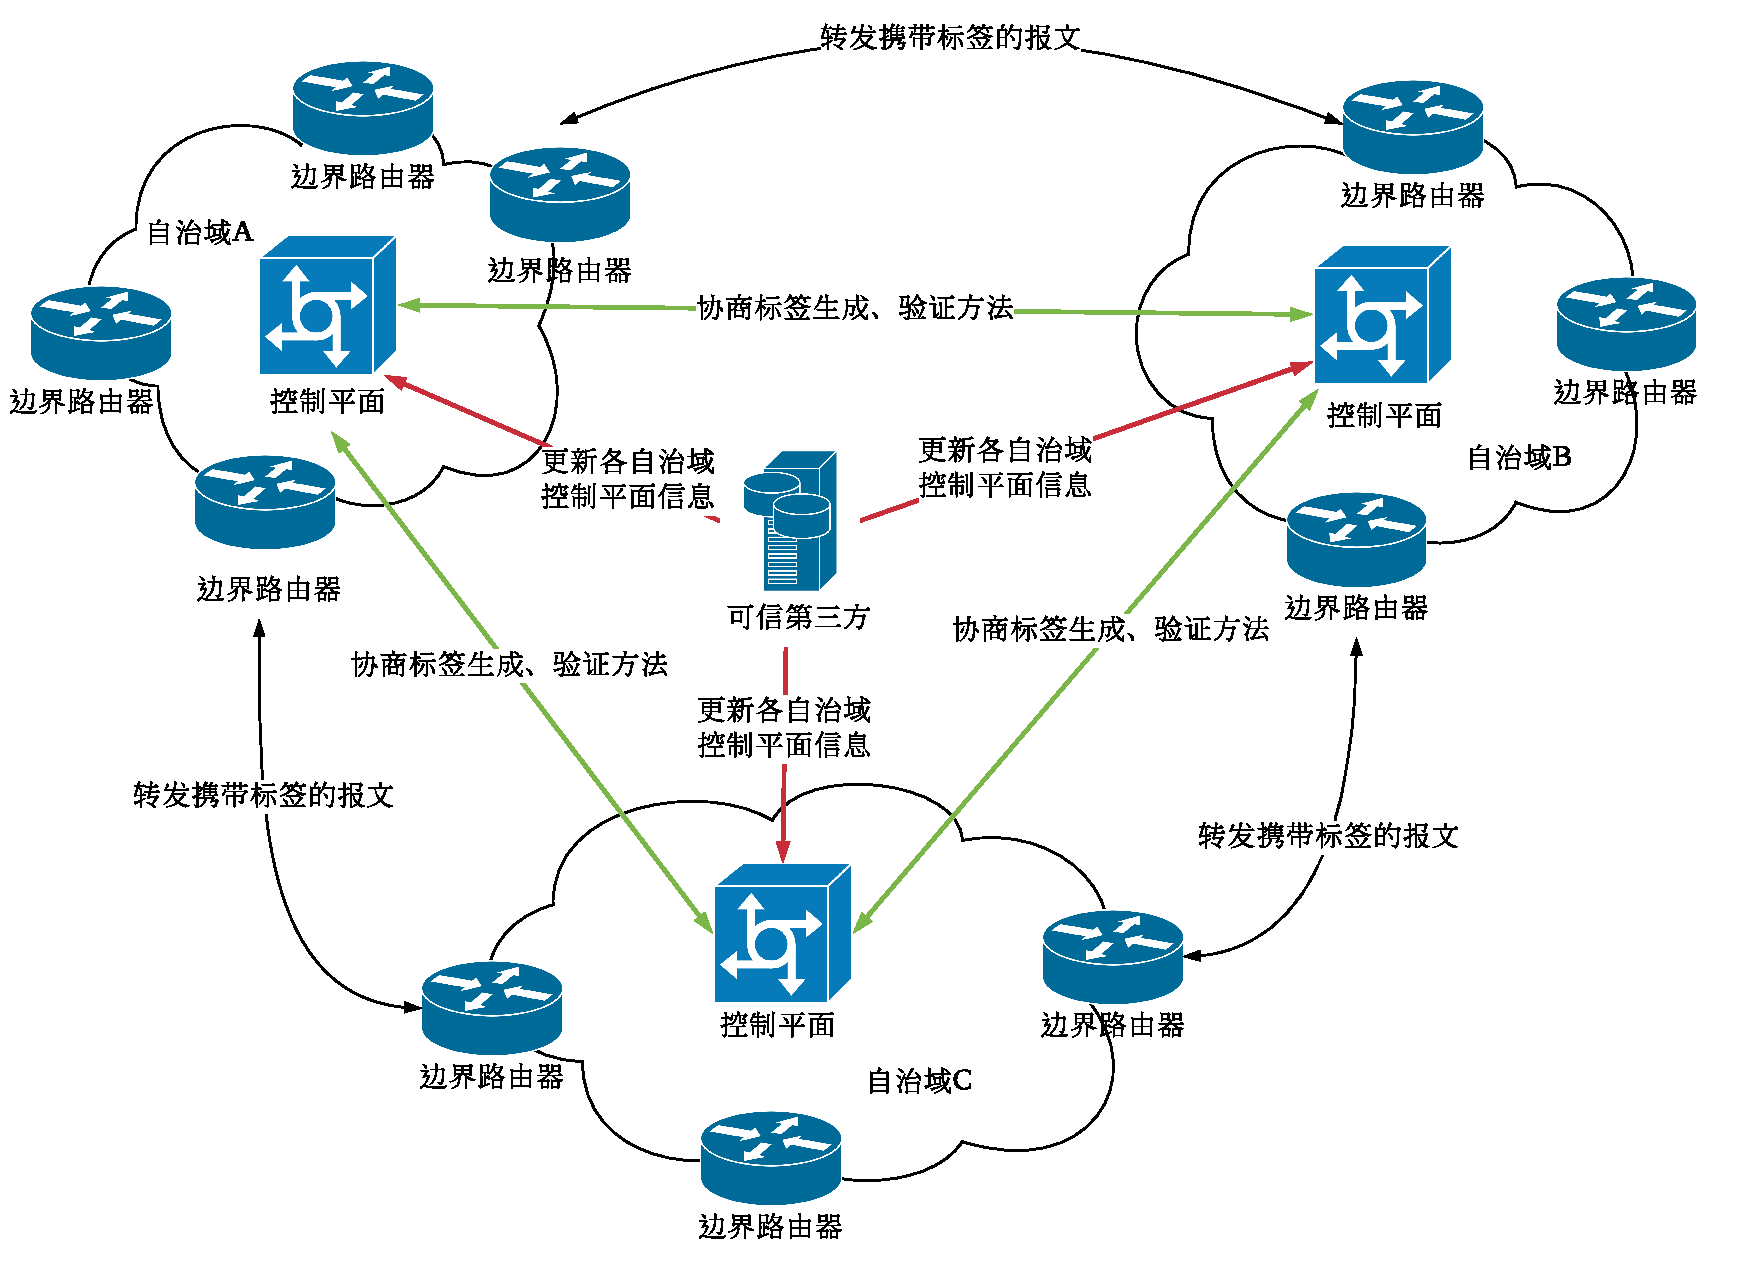
\includegraphics[width=0.7\textwidth]{end_to_end_validation_topology.pdf}
        \caption{端到端验证类自治域间源地址验证方案结构示意}
        \label{fig:end_to_end_validation_topology}
      \end{figure}

      IPSec\cite{RFC2401}中提出的认证头隧道模式在自治域之间建立安全的通信隧道,在完成对端身份校验后,源自治域使用对完整报文进行哈希的方式生成标签并携带在报文中,目的自治域根据协商好的密钥采用同样的哈希算法对报文进行计算并与报文携带的标签进行比较,从而验证完整报文的真实性,其对每个完整报文都进行哈希生成标签的操作,为数据平面带来了较大的性能开销。
      SPM\cite{bremler2005spoofing}采取与IPSec类似的思想生成标签,但其仅对报文的头部进行哈希以降低性能开销,并提出了安全联盟的概念以增强自治域间源地址验证技术的部署激励,即仅有加入安全联盟的自治域才能够享受到自治域间源地址验证技术的安全性保障,从而吸引更多自治域加入安全联盟部署该技术。
      Passport\cite{liu2006efficient}在SPM的基础上,增加了路径检查的功能,要求在报文转发路径上的每个自治域均对报文进行检查,属于一种标签和路径合法性检查并举的方案。这种方式虽然提供了在到达目的自治域前阻断攻击流量的功能,但由于路由动态变化的影响,Passport易导致报文的错误丢弃。
      SMA\cite{shen2008two,bi2009preventing}同样采用基于安全联盟的设计,但使用状态机对数据平面性能做了更进一步的优化,各自治域控制服务器ACS之间定期进行通信协商状态机,而后即采用状态机生成的标签作为报文源IPv6地址真实的背书证据,并通过标签序列的快速变化避免标签被攻击者伪造,避免了数据平面对报文的签名操作。

      总而言之,相较于拓扑验证类自治域间源地址验证方案,端到端类自治域间源地址验证方案的优势主要有:
      \begin{itemize}
        \item 支持增量部署,允许若干自治域先行部署方案并逐步推广。
        \item 安全联盟内自治域间源地址伪造可预防,具备一定部署激励。
        \item 不依赖于网络中运行的其他协议,不受制于依赖协议的安全性。
        \item 不对报文转发拓扑进行假设,不易出现丢弃合法报文的假阳性问题。
      \end{itemize}

      另一方面,端到端验证类源地址验证方案共有的不足之处主要在于:
      \begin{itemize}
        \item 数据平面增加了额外的性能开销。
        \item 控制平面间的协商过程维护较复杂,易发生错误或遭受攻击。
        \item 需引入额外的信任基础维护自治域间通信所需信息,且其功能直接影响到所有跨域报文的转发。
        \item 对于伪造源地址的恶意流量仅能在目的自治域进行阻断,无法消除转发路径上网络资源的损耗。
      \end{itemize}

      \subsubsection{拓扑验证类自治域间源地址验证方案}
      \label{survey:sava:interas:path}
      拓扑验证类的自治域间源地址验证方案是指这样一类技术:网络中各自治域通过一定手段学习跨域报文的合法转发路径,在报文由源自治域路由至目的自治域的过程中,由所经过的各自治域节点对报文转发路径的合法性进行检查,提前过滤源地址与合法转发路径不匹配的报文,如图\ref{fig:topology_validation}所示。

      \begin{figure}[ht]
        \centering
        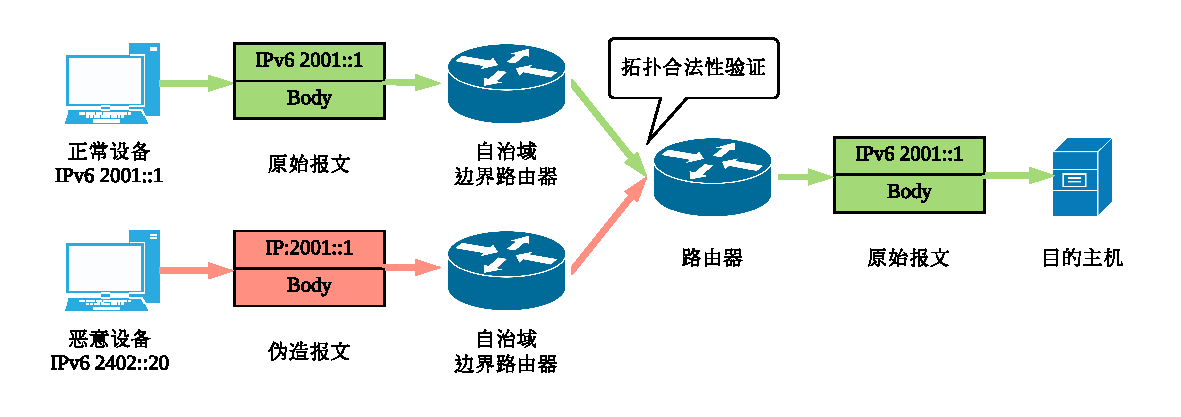
\includegraphics[width=0.9\textwidth]{topology_validation.pdf}
        \caption{拓扑验证类自治域间源地址验证方案原理}
        \label{fig:topology_validation}
      \end{figure}

      IEF(Ingress/Egress Filtering)\cite{RFC2827}通过在各自治域的边界进行出口检查,过滤伪造源IP地址的报文,仅允许本自治域的源IP地址报文转发,在转发路径的起始点进行恶意流量的拦截。但IEF仅能规范自治域自身的行为,而难以预防来自其他自治域的攻击,且需要进行手动配置、增加运维难度,因而难以带来部署激励。
      uRPF\cite{uRPF}针对IEF运维困难的问题,以残桩自治域的拓扑结构作为假设前提,将IEF中过滤伪造报文的关口上移至残桩自治域所上连的自治域,利用BGP协议提供的拓扑信息,自动配置来自残桩自治域的报文的过滤规则,减轻了手工配置的难度与易出错性,但由于互联网环境的复杂与各自治域对可用性的考虑,其残桩自治域的假设不具备普适性。
      IDPF(Inter-Domain Packet Filters)\cite{duan2006constructing}通过假设报文转发路径与BGP Update宣告的路径一致,根据IP前缀路由对报文的不合法转发路径进行过滤。IDPF拓展了方案的使用范围,但其假设过于理想,而网络中存在大量非对称路由,且报文的转发路径很可能随着网络环境的改变而发生实时变化,因此容易造成合法报文的错误过滤。
      SN(Selection Notice)\cite{lijun2006bgp}通过拓展BGP协议,为其新增路由选择公告的报文以在自治域路由规则更新时将其告知对端自治域,路径上的各自治域也通过学习路由选择公告报文来学习新的路径过滤规则。这种方式使报文转发路径中的任一自治域均有对报文进行验证的能力,但其受制于BGP自身的安全,同时其功能的正确运作要求该技术的全局部署,无法支持增量部署的方式。
      SAVE(Source Address Validation Enforcement)\cite{li2002save}设计了一种独立于路由协议的SAVE协议来实现路由路径探测的功能,其通过周期性发送SAVE Update报文建立自治域的入向树,自治域边界路由器则根据入向树的结构生成用于源地址验证的入向表,这种方式解耦了与路由协议的绑定,消除了其他协议带来的依赖安全性,但其正常运作同样依赖于全局部署,并且实现方式过于复杂,难以进行实际的部署。

      总而言之,基于拓扑合法性检查的源地址验证方案虽可以提前过滤伪造源地址的流量,尽可能地增大部署方案所带来的经济收益,但也存在共有的不足之处:
      \begin{itemize}
        \item 拓扑验证规则难以建立;
        \item 许多方案与BGP协议存在耦合,受制于BGP安全性;
        \item 验证规则易受路由动态性的影响,造成报文的错误过滤;
        \item 难以过滤符合拓扑验证规则的源地址伪造报文;
        \item 难以支持增量部署,缺乏推广的可行性。
      \end{itemize}

  \section{IPv6地址生成方案的研究}
  \label{survey:generation}
  由于IPv6允许采取SLAAC方式配置地址,因此网络设备需要能够高效地生成IPv6地址的方案,而IPv6巨大的地址空间,一方面为IPv6地址资源的管理和监测带来了挑战,另一方面也为IPv6地址携带除寻址作用外更丰富的信息带来了可能。IPv6单播地址可分为IPv6子网前缀与接口标识两个组成部分\cite{RFC4291},本节主要综述研究如何生成接口标识的相关方案,其他的地址生成方案例如SIIT\cite{RFC2765}、IVI\cite{RFC6219}等主要研究从IPv4到IPv6地址的翻译过渡技术,而非用户接入IPv6网络时的地址生成方案,因此不在本文的讨论范畴以内。目前已有多种IPv6地址的生成方案被提出,各类方案往往都利用设备或用户身份等信息生成不易冲突的接口标识,但在隐私保护、网络管理、用户审计、路由聚合等方面做了不同的取舍。

  RFC 2464\cite{RFC2464}中提出采用根据IEEE 802定义的48位MAC地址生成EUI-64标识符作为IPv6地址的接口标识。这种生成方式较为简单,但其生成的IPv6地址不发生变化,与用户接口的二层地址相绑定,易造成隐私泄露的问题。
  RFC 4941\cite{RFC4941}针对这一问题提出了临时地址方案,使用加密算法对EUI-64标识符进行哈希后生成接口标识,同时定期更换所生成的IPv6地址。这种方式在一定程度上保护了用户设备的隐私,但增加了网络管理的复杂性。
  RFC 7217\cite{RFC7217}为减轻临时地址方案所带来的网络管理复杂性,提出了一种语义不透明的接口标识生成方法,能够保护用户隐私并提供较为稳定的IPv6地址。
  上述方案均未充分利用IPv6地址空间巨大的优势,使IPv6地址携带更多的语义信息。
  GIRO\cite{oliveira2007geographically}关注IPv6地址的路由聚合问题,提出一种根据地理位置和网络服务提供商对IPv6地址进行生成的方案,以实现相同地理位置、同一运营商内部能够进行较好的路由聚合。
  NIDTGA地址生成方案\cite{liu2015building}针对用户溯源功能进行研究,充分利用IPv6地址空间广阔的优势在接口标识中嵌入对称加密后的用户网络身份标识与时间信息,可在保护用户隐私的同时实现根据IPv6地址追溯用户身份的功能,为建设对恶意攻击者的威慑手段提供了有力支持。

  \section{用户身份认证与溯源技术}
  \label{survey:identity}
  
      \subsection{用户身份认证技术}
      \label{survey:identity:authenticate}
      对用户在接入时进行身份认证的技术一般可分为三类:二层准入认证技术、三层准入认证技术以及客户端技术。
      
      二层准入认证技术的特点是用户设备与认证控制设备之间通过二层的数据帧进行认证信息的传递,用户设备配置IP地址必须发生在用户完成认证之后,在没有完成身份认证前,网络层及以上的报文是无法通过认证控制设备的。PPPoE认证\cite{RFC2516}采用PPP协议通过以太网实施用户接入,为以太网帧提供身份验证的功能,用户设备通过点对点协议与认证控制设备进行链路协商、用户认证信息的提交,由认证控制设备本地认证或通过RADIUS协议去AAA服务器处完成认证。PPPoE认证方式的缺点是需要安装特定的客户端软件,并且其封装代价高,用户认证效率较低。802.1X\cite{ieee802ieee}是更为广泛使用的二层准入认证方式,与PPPoE类似,用户设备通过链路层数据帧与认证控制设备进行通信,但其不需要进行基于以太帧的封装,因此认证的开销较小。本文后续将重点研究基于802.1X作为二层准入认证手段的用户身份识别与溯源系统设计,在此对802.1X的工作原理进行详细介绍。
      
      802.1X认证过程一般涉及用户设备、认证控制设备、AAA服务器三个角色,其中用户设备与认证控制设备之间使用EAP协议帧进行通信,认证控制设备一般将用户的EAP帧封装为RADIUS报文,发送至AAA服务器进行认证。配置了802.1X认证的接入设备,如接入交换机或无线AP等,对于每台用户设备的MAC地址,将虚拟出两个虚拟端口,其中一个被称为非受控端口,仅允许802.1X认证的EAP帧通过,另一个则称为受控端口,用于控制用户其他报文的转发。在设备认证通过前,其仅能通过非受控端口发送EAP协议帧进行用户身份认证。一个典型的认证过程如图\ref{fig:802.1X_authentication}所示:
        \begin{enumerate}[1{)}]
          \item 用户设备连接认证控制设备,建立新的连接,用户设备的802.1X客户端发送EAPOL Start帧,发起802.1X认证的流程。
          \item 认证控制设备处根据用户设备MAC地址对其进行标识,向其回复EAP Request Identity帧,请求使用该设备的用户身份。
          \item 用户在操作系统自带的802.1X客户端上填写用户名与密码,将用户名携带在EAP Response Identity帧中回复认证控制设备;认证控制设备提取EAP Response Identity中的用户名,将其与原EAP帧均封装为RADIUS Access Request报文中的属性后,采用RADIUS协议将认证报文发送给AAA服务器请求认证。
          \item AAA服务器将根据RADIUS报文中携带的用户名属性,提取用户名查询用户数据库,确认存在后向认证控制设备回复RADIUS Access Challenge报文,其中包含回复用户设备的EAP Request帧,用于说明希望用户设备加密用户密码等信息的EAP方法;认证控制设备解封装RADIUS Access Challenge报文,将EAP Request帧转发给用户设备。
          \item 用户设备若同意AAA服务器与之协商的EAP方法,则根据该方式加密用户密码,将密文携带在EAP Response帧中发送给认证控制设备;认证控制设备将其封装在RADIUS Access Request报文中发送至AAA服务器。
          \item AAA服务器收到RADIUS报文后,检查其中携带的EAP Response帧中的密文,与用户数据库中用户密码根据相同加密方式生成的密文相比较,若相同,则回复RADIUS Access Success报文;认证控制设备将提取RADIUS Access Success报文中的EAP Success帧,将其转发给用户设备,并打开用户设备MAC地址对应的受控端口,允许除EAP帧以外的其他类型流量通过。
        \end{enumerate}
    
        \begin{figure}[ht]
          \centering
          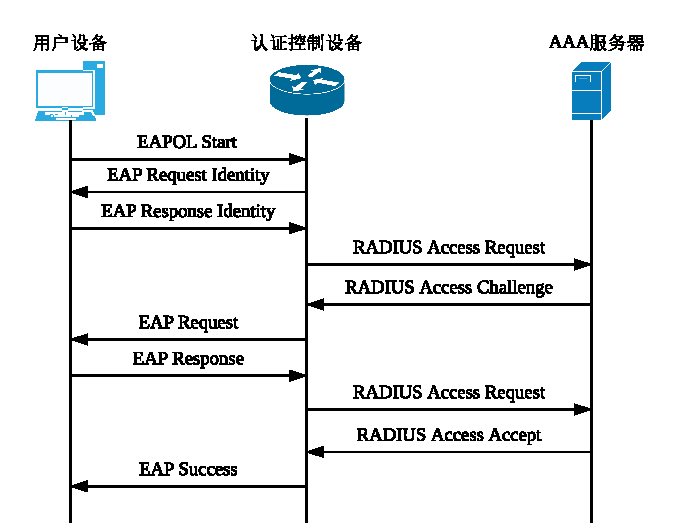
\includegraphics[width=0.8\textwidth]{8021X_authentication.pdf}
          \caption{802.1X认证时序}
          \label{fig:802.1X_authentication}
        \end{figure}
        
      802.1X认证手段的优势在于认证过程安全、认证效率高、设备广泛支持、建网成本低、对无线终端漫游支持较好,但由于其二层认证的特性,仅能支持针对在线时长的计费,难以支持对用户流量的计费。
      
      三层准入认证手段一般通过Web Portal提交用户认证信息。用户首先完成IP地址配置,然后在发送ARP、ND请求过程或通过浏览器访问网络时,触发认证控制设备的认证流程。认证控制设备将用户流量重定向至Web Portal的认证页面,在用户提交用户名、密码等信息完成认证后,Web Portal认证系统向认证控制设备下发用户对应的流量规则,允许用户设备对应的IP地址流量访问外部网络,其一般流程如图\ref{fig:web_portal_procedure}所示。目前Web Portal认证虽然在实际网络中广泛使用,但均为厂商内部实现,并未形成统一的国际标准。
      
      \begin{figure}[ht]
        \centering
        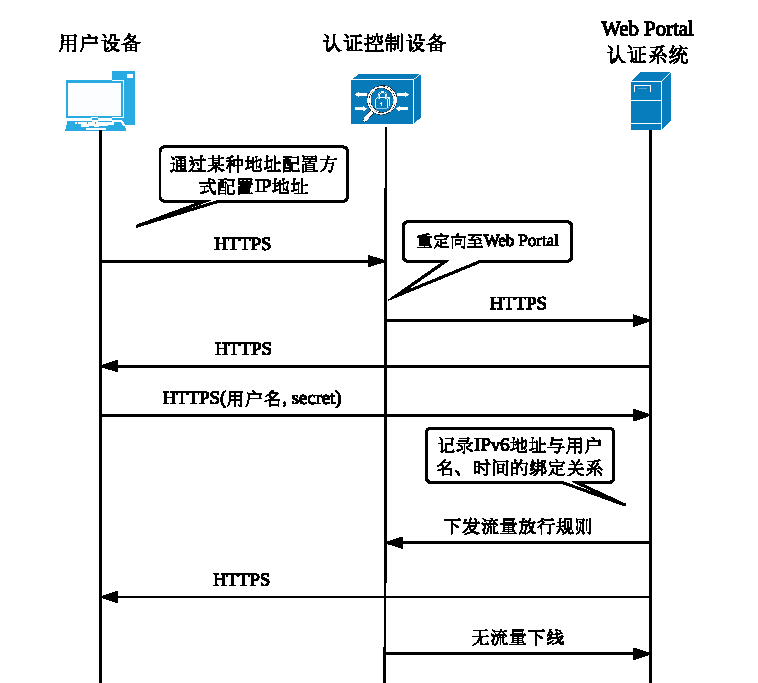
\includegraphics[width=0.8\textwidth]{web_portal_procedure.pdf}
        \caption{Web Portal认证时序}
        \label{fig:web_portal_procedure}
      \end{figure}
      
      Web Portal认证手段的优势在于不依赖于客户端、便于用户身份与IP地址的绑定、能够支持流量计费,但其安全性较弱,与用户的连接性差,不能很好地支持用户漫游的场景,组网的成本高,并且认证流程与交互信息没有规范化,未形成国际标准。
      
      客户端认证手段则是指一类在用户设备上安装特定软件以实施用户接入功能的身份认证方式。一般而言,客户端认证均是利用定制客户端替代操作系统内核某一模块功能,在其原生模块功能之上增加一定的功能扩展,如用户身份认证、设备安全性检查等,以实现个性化定制认证流程的功能。这种方式灵活性较强,可能可以提供更强的安全性,但其开发工作量大,推广部署困难,并且其私有化程度高,引入新的安全问题的风险更大。
  
      \subsection{用户身份溯源技术}
      \label{survey:identity:trace}
      目前根据IP地址对用户身份进行追溯的方法主要有两种。一种是在利用Web Portal进行用户身份认证的网络中常见的IP地址与用户身份绑定方案,另一种则是NIDTGA地址生成方案提出的用户身份溯源方法。
    
      Web Portal进行用户身份与IP地址绑定的溯源方案原理比较简单,由于用户认证时需要使用IP地址访问Web Portal网站,因此可以轻易地将用户IP地址与用户认证的身份关联并存储以支持后续的溯源。其能够支持各种IP地址配置方式,但为实现溯源功能必须存储所有历史绑定记录,存储开销较大,并且在IP地址资源进行时分复用的情况下,仅凭IP地址难以确定实际的用户身份,必须配合IP分组的时间信息,为用户身份的溯源带来困难。此外,其方案限定了Web Portal认证的方式,在无线网络发展繁荣的今天难以良好地支持无线终端的移动性要求,而在采用二层准入认证的网络中又难以实现IP地址与用户身份的绑定,不具备较好的推广能力。
    
      NIDTGA地址生成方案\cite{liu2015building}在用户认证时通过IDEA对称加密的方式为其生成嵌入了用户身份与认证时间的IPv6地址,在用户请求配置地址时将其配置给用户设备。在有用户身份溯源需求时,使用密钥更新历史对待追溯的IPv6地址进行解密,以获得用户身份信息,其具体原理如图\ref{fig:NIDTGA_procedure}所示:
      \begin{enumerate}[1{)}]
        \item 组织管理员根据用户在现实生活中的身份标识(如身份证号、学号等)为用户生成一个长度为40位二进制的用户网络身份标识NID。
        \item 用户所在组织的管理域为用户生成IPv6地址时,将NID与当前的时间信息拼接成一个长度为64位二进制数的原文,采用IDEA加密方法根据某一个组织管理员设定的密钥加密获得一个长度为64位二进制数的密文。
        \item 将密文作为接口标识,与用户设备所在子网的IPv6子网前缀拼接,形成用户设备的IPv6地址。
        \item 追溯时,审计方首先根据IPv6地址前缀确定用户所在的组织,获取该组织使用过的IDEA密钥历史。
        \item 根据组织IDEA密钥历史,从最新的密钥开始,按照历史记录往前逐一使用当前密钥对用户IPv6地址的接口标识进行解密,从解密获得的64位原文中提取时间信息。
        \item 比较提取的时间信息与当前解密用密钥的有效时间,若时间信息位于密钥的有效时间内,则说明该IPv6地址接口标识确实由该密钥加密生成,提取接口标识原文中的NID段获得用户身份标识NID。
      \end{enumerate}
    
      \begin{figure}[ht]
        \centering
        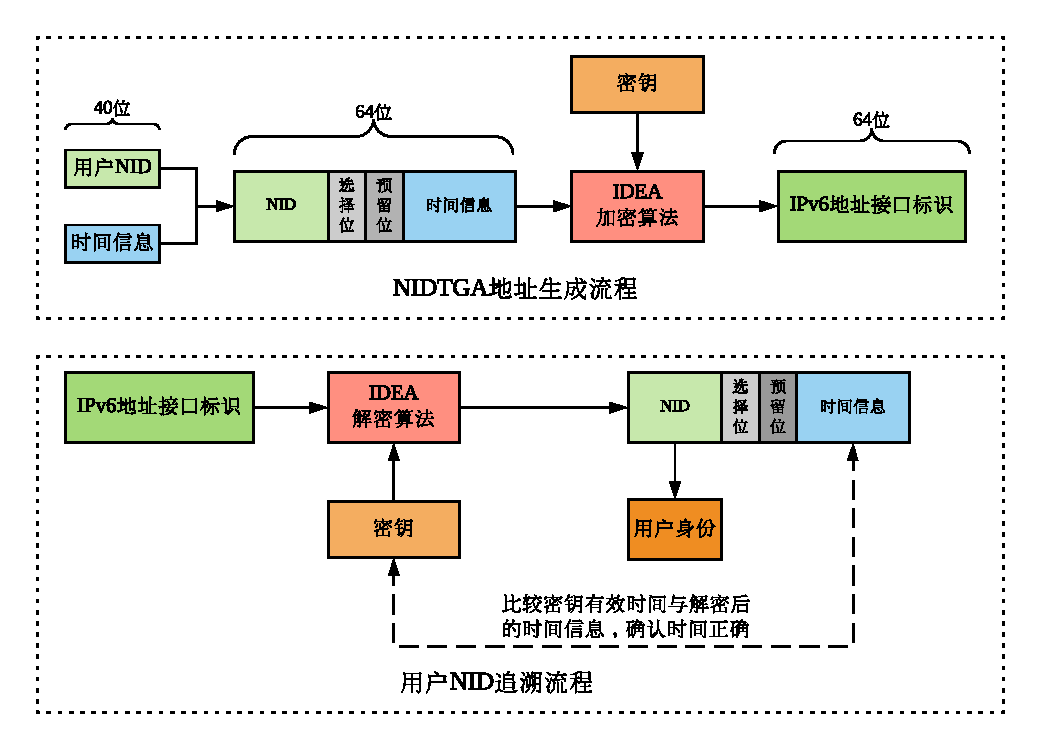
\includegraphics[width=0.9\textwidth]{NIDTGA_procedure.pdf}
        \caption{NIDTGA地址生成与追溯过程}
        \label{fig:NIDTGA_procedure}
      \end{figure}
    
      NIDTGA地址生成方案将用户身份与时间信息均携带在IPv6地址内部,无需进行IPv6地址与用户身份绑定关系的存储,节省了存储开销,在溯源时无需确定恶意分组的时间信息,避免了身份溯源的错误,增添了溯源能力的便利。其统一的用户身份标识NID设计,也为跨管理域的用户身份统一溯源奠定了基础,有利于该技术的推广。但是,其未对接入网络中复杂的用户认证与地址配置的结合方式加以详细的考虑,因此采用NIDTGA地址生成方案的用户身份识别与溯源系统在实际网络环境中的设计与实现仍亟待研究。

  \section{区块链的相关研究}
  \label{survey:blockchain}

    \subsection{区块链原理}
    \label{survey:blockchain:theory}
    区块链的本质为一个分布式数据库,其记录的数据内容被分散地备份在区块链网络中每一个完整的区块链节点上,所有节点之间通过共识算法达成对数据库中数据的共识。其记录数据的方式不同于传统的关系型数据库支持数据的本地修改,而是更接近追加型的NoSQL,仅能向其中写入新的数据而无法对已写入区块链的数据进行更改。与普通的追加型NoSQL数据库有别的是,区块链将数据进行分块,存储为首尾相连的链表格式,并使用密码学技术确保攻击者难以承受篡改数据的代价以规避数据被篡改的可能。向区块链中写入新数据的过程并非分布式系统中常用的主从复制模式,而是往往通过一些资源拥有证明的方法来处理数据写入的权力分配,当攻击者无法占有区块链网络中大部分的资源时,它就无法垄断区块链中数据写入的权力,因此可以被应用于拜占庭情况下的网络环境中。由于区块链最初诞生于加密货币领域,被用于交易的记账,因此人们更多地称其为分布式账本。

    一个典型的区块链结构如图\ref{fig:blockchain_structure}所示。整个区块链呈一个链表状的结构,链表中每个节点都是一个区块(Block),区块之间依次相连,新的数据将组成一个新的区块添加到链表的末尾,指向先前的区块。以比特币的区块链为例,其每一个区块分为区块头(Block Header)与区块体(Block Body)两部分。区块头中记录了区块版本、前一区块的哈希值、Merkle树\cite{merkle1987digital}根节点、时间戳以及随机数答案等,区块体中记录了这一区块出块过程中发生的交易(Transaction)数量和每笔交易的信息。

    \begin{figure}[ht]
      \centering
      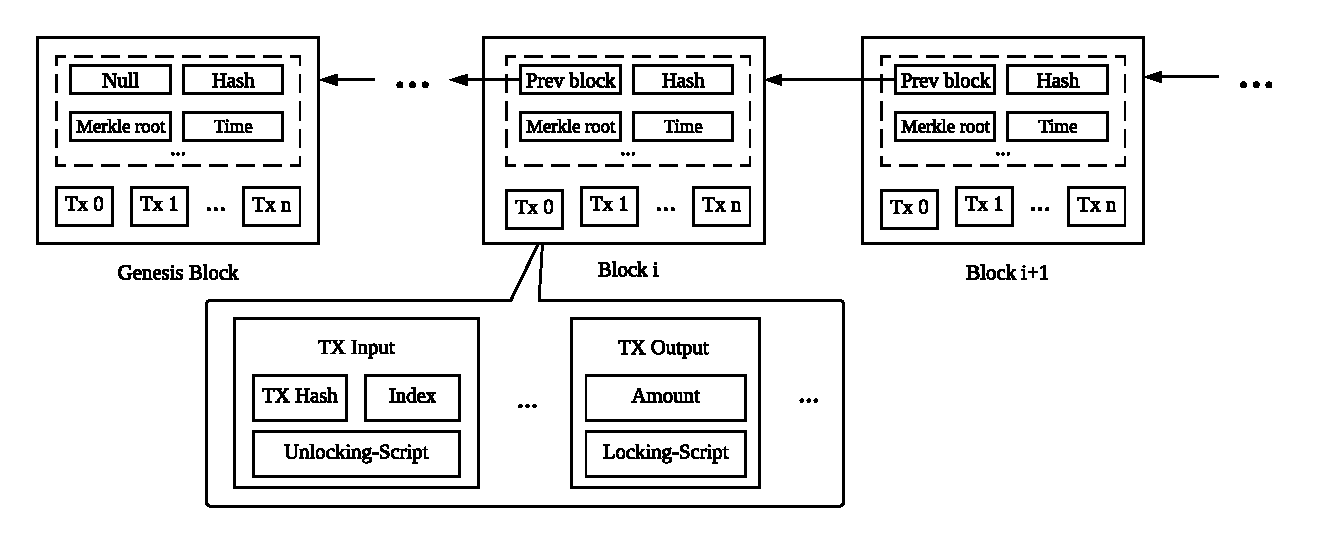
\includegraphics[width=0.9\textwidth]{blockchain_structure.pdf}
      \caption{区块链结构示意}
      \label{fig:blockchain_structure}
    \end{figure}

    用户要与区块链进行交互,首先需要创建其钱包。所谓钱包,其实就是一个公私钥对,钱包的地址由公钥经过一系列数字签名运算后得到。区块链使用公私钥对来确保交易的合法性。当用户有新的数据想要写入区块链时,其首先使用私钥对包含了数据的交易进行签名,然后通过区块链节点广播到整个区块链网络中。网络中的其他节点将使用交易发起者的公钥对交易签名进行验证,从而保证交易在传播途中没有遭到篡改。

    当有新的数据需要写入区块链中时,区块链网络中的各个节点会通过一种名为挖矿(Mining)的方式对新区块中的内容达成共识,参与挖矿的节点被称为矿工(Miner)。挖矿过程中采用的共识算法有非常多种,但最广为人知且得到良好实践的一种即为比特币所采用的工作量证明(Proof of Work,PoW)方法。以比特币为例,其工作原理如下:
    \begin{enumerate}[1{)}]
      \item 矿工节点收集到足够多的合法交易后,其将这些交易打包为一个区块,并生成包含前一区块哈希值、本区块所包含交易的Merkle树根、时间戳等信息的区块头,并开始计算如下的工作量证明难题:寻找区块头中的随机数答案nonce值,使得将80个字节的区块头作为输入送给SHA256\cite{burrows1995secure}算法进行哈希后,所得到的答案小于区块链网络当前的目标值。当前目标值由式\eqref{eq:blockchain_pow_adjustment}进行调整。设区块链网络设定的最大目标值为$M$,当前难度值为$d$,则目标值$o$由式\eqref{eq:blockchain_target}确定。比特币网络每产生2016个区块即会根据其运行状态调整难度值$d$,设原本的难度值为$d'$,过去生成2016个区块的总时间为$t$,则新的难度值$d$由
      式\eqref{eq:blockchain_difficulty}确定,以保证整个比特币网络始终以约每十分钟一个区块的速度产生区块。
      \begin{subequations}
        \label{eq:blockchain_pow_adjustment}
        \begin{align}
          o &= \frac{M}{d} \label{eq:blockchain_target}  \\
          d &= d' * \frac{t}{2016*10} \label{eq:blockchain_difficulty}    
        \end{align}
      \end{subequations}
      \item 矿工将持续不断地尝试改变nonce值并进行SHA256计算,直至寻找到一个满足SHA256$(block\_header) <= o$的nonce值。一旦找到,矿工立即将其填入区块头中的对应字段,向比特币网络广播新区块。
      \item 网络中其他节点收到广播的新区块时,将对其区块头进行校验,检查内容包括该区块头所包含的哈希值是否与其高度的前一个区块一致、宣告的答案是否满足当前网络的工作量证明约束等,然后验证新区块中每一笔交易的合法性,若全部校验通过,则节点将该新区块加入到自身维护的区块链中。
    \end{enumerate}

    由于区块链中采用链表的形式对数据进行组织,每一个区块中都包含有前一区块数据的哈希值,因此如果攻击者想要欺骗整个区块链网络,使其他诚实的区块链节点对某一区块中的伪造数据达成共识,其需要对自该区块开始往后的全部区块重新进行工作量证明的计算,而工作量证明难题确保了挖矿能力与节点的算力成正比,因此没有掌握全网一半以上算力的攻击者无法对已经形成共识的区块链数据进行篡改,从而保障了区块链中数据不受篡改的特性。

    同时,由于区块链中数据的全量副本均分布在每一个区块链节点上,其天然拥有容灾备份的优势,可以极大提高数据的可靠性。

    \subsection{区块链技术的发展}
    \label{survey:blockchain:development}
    在比特币网络中,区块链仅仅作为一个分布式账本对比特币转账交易进行记录,尽管其能够执行一些脚本命令,但所支持的功能是十分受限的,因而难以在其上构建除加密货币外的其他应用。

    针对这一问题,以太坊\cite{wood2014ethereum}提出了以太坊虚拟机(Ethereum Virtual Machine,EVM)与图灵完备的Solidity语言。使用Solidity语言编写的智能合约能够实现用户自定义的应用逻辑,并被部署到以太坊网络在EVM内部执行。由于这种应用分散于整个以太坊网络的各个节点,因而常被称为分布式应用(Distributed App,DApp)。当用户发起交易时,交易可以定义创建合约、调用合约、向合约转账等功能的各种逻辑。由于合约的执行需要消耗节点的资源,因此为了使自己的交易能够被矿工节点打包入区块中,用户需要向矿工节点支付一种名为Gas的费用,以用户愿意支付的以太币(Ethereum,ETH)价格为单位进行衡量。在EVM内部,每一条指令的执行都有其对应消耗的Gas数量,矿工节点将根据用户交易中提供的价格来计算将交易打包进区块所要收取的Gas总价。每一个以太坊节点中的区块链都会记录智能合约的代码与状态,当节点需要验证新的区块时,对于区块中有合约交互的交易,以太坊将根据交易顺序在EVM中依次执行交易中调用的合约逻辑,若出现代码执行错误或消耗的Gas总量超出用户交易规定的上限时,新区块的验证失败,EVM将终止智能合约的执行,并将区块链回滚到未验证新区块之前的状态。以太坊的诞生,使区块链的跨领域应用成为可能,引发了世界范围内开发者在其上构建DApp的热潮,形成了繁荣的以太坊生态。但是,以太坊仍存在以下缺陷:
    \begin{itemize}
      \item 目前的以太坊网络仍采用PoW共识方法,尽管可以根据难度值的调整缩短达成共识的时间,但其上智能合约的调用仍是异步的过程,难以媲美传统应用同步调用的性能;
      \item 在以太坊上构建DApp必须使用Solidity这一领域限定语言,而不支持类似于Java、Go等非领域限定的高级语言,对DApp的开发造成了一定的壁垒。
    \end{itemize}

    与比特币、以太坊不同,超级账本技术\cite{dhillon2017hyperledger}致力于采用区块链技术解决非公开网络中的数据安全问题,其应用场景并非完全不可信的参与方,而是互相之间具有信任基础的联盟体。因此其在区块链的性能与数据安全性之间做了一定取舍,并采用容器技术支持了通用高级语言的执行。Fabric\cite{androulaki2018hyperledger}采用Kafka\cite{thein2014apache}或Raft\cite{ongaro2014search}共识算法替代了PoW,优化了共识算法的性能,但舍弃了对恶意节点接入的防御能力。其提出了账本节点、排序节点等多种节点角色,支持节点之间创建Channel,在同一个Fabric网络中构建多个分布式账本,以更好地满足联盟链场景下的需求。Fabric对高级语言的支持更为充分,支持开发者使用Java、Go与Node.js开发分布式应用并在容器Docker中运行,降低了区块链开发的门槛。Besu\cite{Besu}在以太坊的基础上引入了IBFT、Clique等权威证明的共识机制,并为联盟链和私有链场景设计了更为友好的以太坊客户端以适应企业的需求。Indy\cite{Indy}为区块链上的数字身份互操作场景提供了可重用组件的解决方案。Sawtooth\cite{Sawtooth}设计了一种灵活的模块化区块链体系结构,支持用户应用在无感知的情况下可自由地替换底层区块链组件,支持实用拜占庭算法(Practical Byzantine Fault Tolerance, PBFT)\cite{castro1999practical}与经过时间证明算法(Proof of Elapsed Time,PoET)\cite{rilee2018understanding}。超级账本技术对于企业联盟或私有场景提供了比以太坊更为丰富的工具与功能支持,并且往往都支持非领域限定的高级语言进行开发,但其一般采用非PoW的共识算法,虽提升了共识效率,但存在一定程度的中心化特点,削弱了对数据真实性的保护。

  \section{本章小结}
  \label{survey:summary}
  本章从IPv6地址配置方式开始,对实现和部署用户身份识别与溯源系统所需要支持的地址配置场景进行了全面的介绍。同时,对作为用户身份识别与溯源系统依赖基础的源地址验证技术相关研究进行了讨论,指出了接入子网SAVI技术与自治域间端到端类验证方案存在的一些问题。然后分析了各种IPv6地址生成方案的侧重点,介绍了目前唯一一种以用户身份溯源为目的设计的NIDTGA地址生成方案。接着介绍了目前网络中常见的用户身份认证手段与身份溯源方案,讨论了传统的IPv6地址与用户身份绑定方式的问题,说明了采用NIDTGA方案实现用户身份识别与溯源系统的必要性。最后介绍了区块链技术的原理和发展,启发了本文使用区块链提升域间源地址验证技术与用户身份识别与溯源系统跨组织部署时的安全性,并为开发实现时的区块链平台选择提供了参考。




% !TeX root = ../main.tex

\chapter{IPv6源地址验证技术增强方案}
\label{IPv6_Security}

  \section{本章引言}
  \label{IPv6_Security:introduction}
  网络中的源地址真实是实现用户身份识别与溯源的前提。只有保证了源地址的真实,并将真实的IP地址与用户身份正确地进行绑定,才能够实现通过分析攻击流量定位源IP地址、根据源IP地址溯源攻击者实体的功能。
  按照源地址验证体系结构SAVA的划分层次,接入子网、自治域内和自治域间均可能发生源地址的伪造情况。接入子网作为最靠近用户的层级,其能够提供最细粒度的源地址伪造过滤机制,具有最为基础且深刻的作用。理想情况下,当所有自治域内所有接入子网均能确保不发生子网内的源地址伪造时,自治域内与自治域间的源地址伪造问题便已不复存在。但是,在实际的网络中,自治域间不属于一个管理域,其安全技术的选择与部署包含着自身的利益考虑,不可能进行整体的协调,因此仍需要SAVA中各级机制互相配合以在设备粒度、子网粒度与自治域粒度三个层次预防IPv6源地址的伪造。

  对于基于IPv6地址追溯用户身份的用户身份识别与溯源系统而言,由其提供网络接入服务的用户子网必须要求设备粒度的源地址真实性验证,以确保IPv6源地址可以准确地关联到需要对报文负责的用户实体。自治域内与自治域间也需要提供预防系统部署子网IPv6地址遭到伪造的机制,以保证使用用户身份识别与溯源系统接入的用户不会因为被其他子网或其他自治域的恶意用户假冒地址而被错误追责。

  目前,接入子网的源地址验证技术SAVI已基本全部被标准化,但其在网络中实际部署应用时仍可能面临厂商设备尚未支持或版本过旧、替换或升级成本较高等问题,对用户身份识别与溯源系统的部署使用造成一定阻碍。同时,源地址验证作为一项解决网络安全问题的基础技术,其本身也可能成为恶意攻击者的攻击目标。本章首先分析SAVI技术部署在实际网络中面临的困境,利用传统设备普遍支持的VLAN功能,提出在已有网络环境中以较小代价支持接入子网源地址伪造预防的增强方案,然后针对自治域间源地址验证这一层次,研究其目前一类基于端到端验证思路的主流方案所共有的安全隐患,以其中典型的SMA为例,提出了基于区块链的增强方案设计,并进行了实现与测试,为端到端类域间源地址验证技术提供了统一的安全性改进思路。

  本章内容组织如下:第\ref{IPv6_Security:access}节分析为用户身份识别与溯源系统提供基础支持的SAVI技术在部署时的要求与困境,并提出了在难以进行接入交换机SAVI全支持的网络中实现接入子网内IPv6源地址防伪造的增强方案设计;第\ref{IPv6_Security:interas}节以SMA方案为例对端到端验证类思想的域间源地址验证技术的安全性进行分析,针对SMA方案中REG中心化设计的问题,研究了其联盟注册系统的区块链设计方案RegChain,并在以太坊平台上进行了实现与验证;第\ref{IPv6_Security:summary}节对本章内容进行总结。

  \section{接入子网源地址验证技术增强方案}
  \label{IPv6_Security:access} 

    \subsection{SAVI技术的部署与分析}
    \label{IPv6_Security:access:deploy}

    为了发挥SAVI技术的作用,子网内部署SAVI的设备必须形成一个安全边界,以确保所有设备发出的数据报文在通过子网网关转发前必定经过一台SAVI设备对源地址进行检查。SAVI设备形成的安全边界越靠近用户设备,则能够实现的源地址过滤粒度越精细。如\ref{survey:sava:access:bound}节所述,当有线网络中SAVI安全边界某一个端口下不止一台用户设备时,由于用户设备均对应同一个绑定锚,SAVI设备难以根据IP地址与绑定锚的绑定关系区分来自不同设备的流量,因而难以防止设备之间互相伪造源地址。

    因此,要实现接入子网内不发生源地址伪造,必须由直接连接用户、提供接入的接入交换机或无线接入点部署SAVI、实施伪造源地址报文的过滤:
    \begin{enumerate}[1{)}]
      \item \textbf{无线网络}:在基于无线控制器的集中控制组网方式下,只需要在AC上对接入子网配置SAVI的启用,并根据子网内地址配置方式启用DHCPv6 Snooping或ND Snooping即可。目前华为、新华三等几大设备厂商生产的AP与AC均已支持无线SAVI技术。
      \item \textbf{有线网络}:所有包含接入子网端口的接入交换机全部启用SAVI,确保安全边界端口下连仅有一台用户设备。对于用户在网络管理员所能控制的交换机端口下仍私接交换机的情形,我们认为这是用户的非法行为,发生其下多台设备之间的互相伪造最终被判定由同一用户负责是符合情理的处理结果。
    \end{enumerate}

    但是,在推动各所高校进行接入子网源地址验证技术的部署时,SAVI技术很难做到上述理想情况的部署。对于无线网络,由于不存在链路实体,用户设备通过射频信号与AP进行链路建立和通信,因此即使网络环境中存在版本过旧而不支持SAVI技术的AP,我们仍可以简单地选择不在其上开设进行源地址验证的接入子网的信号。而对于有线环境,情况则较为复杂,网络中接入交换机数量众多,品牌、型号各异,极有可能存在部分接入交换机支持SAVI而另一部分不支持的情况,对于地理位置相近、身份类别相同的用户,由于其上连的接入交换机对SAVI的支持情况不同而为其划分不同的子网、提供不同的接入服务,容易造成用户不良的体验,因此仍需提出在难以将接入交换机全部替换以支持SAVI的情况下如何对非SAVI接入交换机接入用户同样进行IPv6源地址验证的增强方案。

    \subsection{基于VLAN划分的SAVI部署增强方案}
    \label{IPv6_Security:access:enhance}
    尽管将接入交换机全部替换为支持SAVI的设备可能成本较高,但为了部署SAVI技术,必须要在网络中形成安全边界,因此对于非SAVI交换机,其上连至网关的链路中必须有一台交换机支持SAVI。对于二层交换机多级连接的情况,尽量替换靠近用户设备层级的交换机,在最坏情况下,汇聚交换机下所有交换机均不支持SAVI,则汇聚交换机必须支持SAVI。在构成了SAVI安全边界的前提下,若接入子网中存在不支持SAVI的接入交换机,我们可以通过配合特殊的VLAN划分方法实现整个接入子网内的源地址防伪造方案,如图\ref{fig:SAVI_enhance}所示。

    \begin{figure}[ht]
      \centering
      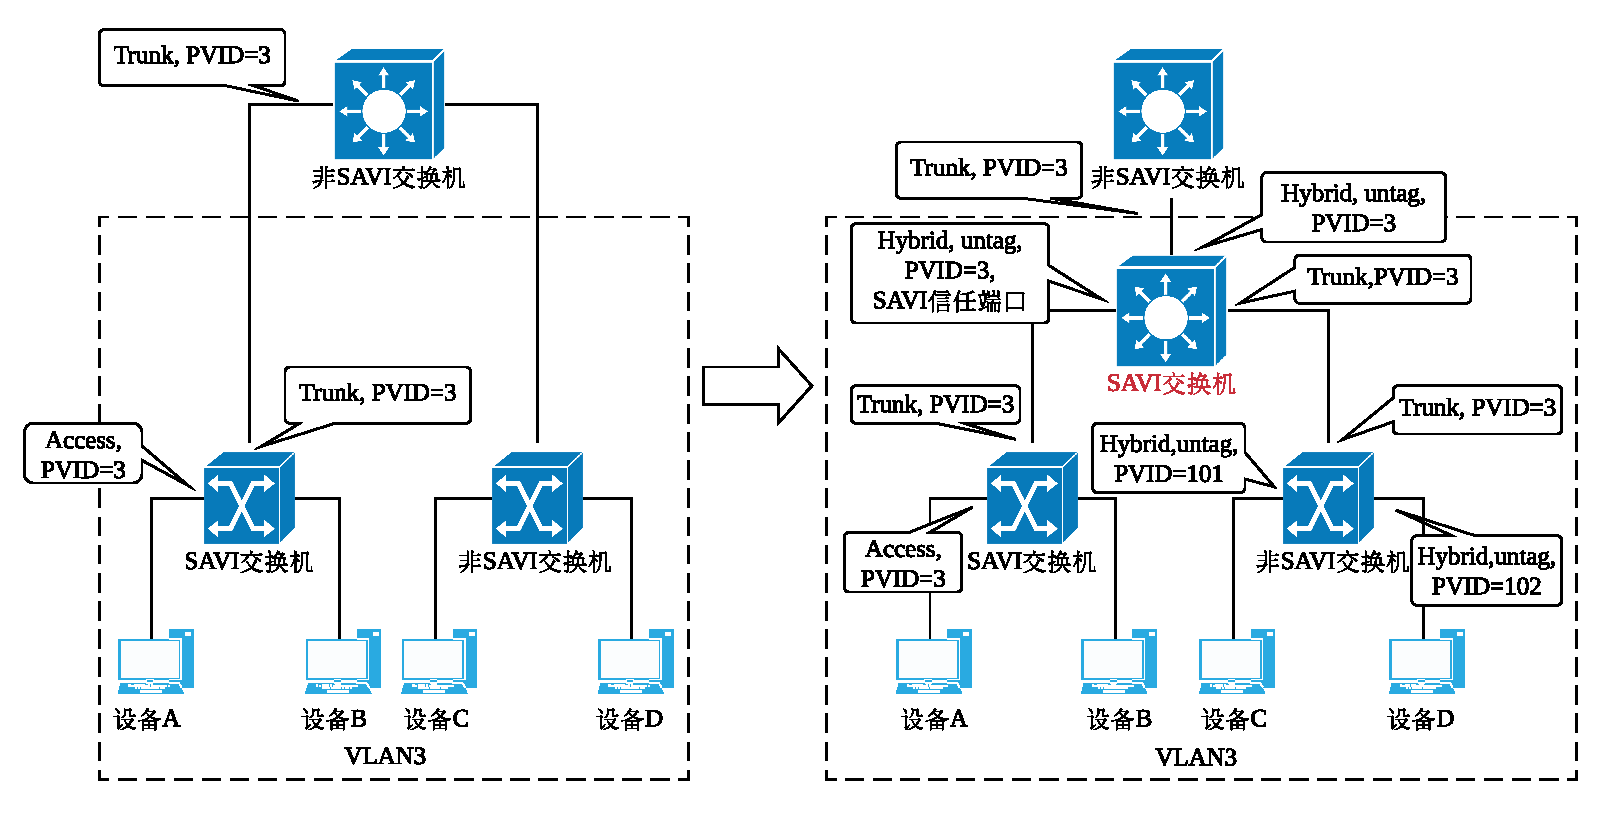
\includegraphics[width=\textwidth]{SAVI_enhance.pdf}
      \caption{基于VLAN划分的SAVI部署增强方案示意}
      \label{fig:SAVI_enhance}
    \end{figure}

    图\ref{fig:SAVI_enhance}左侧为一个有线网络典型的组网拓扑,子网网关位于汇聚交换机上,汇聚交换机下连接有多台接入交换机,接入交换机的端口将直连用户有线设备,提供有线网络的接入服务。一般而言,汇聚交换机数量较少,比如在一栋楼宇中部署一台,而接入交换机则数量众多,一个房间可能就部署不止一台。左图所示接入交换机中,部分不支持SAVI技术,将其全部替换为支持SAVI的设备需要较大的费用开销与网络迁移工程。显然,对于左侧的VLAN 3这一子网,由于SAVI设备没有构成安全边界,仅有设备A、B不可伪造源地址,设备C与D不仅可以互相伪造对方的地址,也可以伪造设备A与B的源地址以及任意其他IPv6地址,无法提供接入子网IPv6源地址的真实性保障。

    如\ref{survey:sava:access:listen}节所述,在有线网络中,SAVI会以源地址与VLAN为索引建立绑定表项,因此图\ref{fig:SAVI_enhance}右侧结合VLAN信息提出IPv6源地址验证的增强方案。首先,虽然无法将所有不支持SAVI的接入交换机进行替换,但我们在接入层与汇聚交换机之间新增一台SAVI交换机(红字标注),即可构成SAVI所要求的安全边界。此时,尽管仍然无法防止设备C与设备D之间互相的源地址伪造,但已大大缩减了它们所能伪造的地址范围,从整个IPv6地址空间缩小到了SAVI交换机下接入的各个设备的源地址,当然也保障了设备A与B的源地址不会被同子网内的其他设备所伪造。然后,我们通过图示的VLAN划分手段,来防止设备C与D之间的互相伪造问题。首先以设备C为例,考察其上行流量与下行流量所携带的VLAN标签:
    \begin{itemize}
      \item \textbf{上行流量}:由设备C发出的报文到达接入交换机后,根据Hybrid端口的检查规则,由于其不带有VLAN标签,交换机向其中加入101号VLAN标签;在允许VLAN 101经过的上连Trunk口,经过Trunk口检查规则,与其PVID=3不匹配,因此保持VLAN号101向上转发;到达SAVI交换机的下连Trunk口时,与其PVID=3不匹配,仍保持VLAN号101;由上连至原汇聚交换机的Hybrid口发出时,由于该端口配置了untag,因此VLAN号101被剥离,在到达汇聚交换机的PVID=3的Trunk口时被重新打上VLAN号为3的标签,进行后续转发。
      \item \textbf{下行流量}:由汇聚交换机向下转发的流量在下连的Trunk口被剥离VLAN号3的标签,在进入SAVI交换机的Hybrid口时被重新加上3号VLAN的标签;在转发至接入交换机时同样在下连的Trunk口剥离3号VLAN标签,由接入交换机的上连Trunk口加入3号VLAN标签;在转发至设备时,设备C所连接的Hybrid端口允许3号VLAN报文通过,并根据untag的配置将其VLAN号剥离后进行转发。
    \end{itemize}

    可见,由设备C发出的报文在到达SAVI交换机时将携带101号VLAN标签,而在到达子网网关时将携带3号VLAN的标签,其内部的101号VLAN对于接入子网外部而言不可见。对于由汇聚交换机下发的报文,其3号VLAN标签将在最终到达用户设备时被剥离,从而使设备网卡能够正常识别并进行处理。在这种情况下,在新增的设备开启SAVI功能后,设备C与设备D互相之间的源地址伪造也将被避免:
    \begin{enumerate}[1{)}]
      \item 当设备C配置IPv6地址时,新增的SAVI交换机将其IPv6地址、VLAN号101与其下连端口相绑定。同样,设备D配置的IPv6地址也将与VLAN号102、下连同一端口相绑定。
      \item 当设备C伪造设备D的MAC地址与源IP地址向外发送报文时,其报文在经过接入交换机端口后将携带VLAN号101到达SAVI交换机。
      \item SAVI交换机根据SAVI绑定表,检查报文中的IPv6地址、VLAN号、MAC地址与端口号,发现虽然IPv6地址、MAC地址与端口号绑定一致,但VLAN号101与绑定表中IPv6地址所绑定的102号VLAN不匹配,说明该报文为源地址伪造报文,将其丢弃。
    \end{enumerate}
    
    因此,在无法实现接入交换机全部部署SAVI技术的情况下,本文给出了一种结合VLAN实现IPv6源地址验证增强的方案,防止了SAVI安全边界下各个设备之间互相的源地址伪造。方案的部署要求总结如下:
    \begin{itemize}
      \item \textbf{新增设备}:在接入层与汇聚层之间新增支持SAVI的交换机,开启SAVI功能。
      \item \textbf{VLAN划分}:位于SAVI安全边界下方的所有设备,其接入有线网络的端口全部配置不同的VLAN号。设子网内所有接入端口配置的VLAN号与子网VLAN号构成的集合为$S$。
      \item \textbf{非SAVI接入交换机下连端口}:接入端口配置子网内唯一的VLAN号,端口类型为Hybrid,允许通过的VLAN号为集合$S$,设置untag,在发送流量时剥离VLAN标签。
      \item \textbf{非SAVI接入交换机上连端口}:端口VLAN号与子网VLAN号相同,类型为Trunk,允许通过的VLAN号为集合$S$。
      \item \textbf{新增SAVI交换机下连端口}:端口VLAN号与子网VLAN相同。连接非SAVI交换机的端口类型为Trunk,连接SAVI交换机的端口类型为Hybrid并设置untag与SAVI信任端口,两者允许通过的VLAN号均为集合$S$。
      \item \textbf{新增SAVI交换机上连端口}:端口VLAN号与子网VLAN相同,类型为Hybrid,允许通过的VLAN号为集合$S$,设置untag,在发送流量时剥离VLAN标签。
      \item \textbf{汇聚交换机下连端口}:端口VLAN号与子网VLAN相同,类型为Trunk,允许通过的VLAN号为子网的VLAN。
    \end{itemize}

    \subsection{SAVI部署增强方案讨论}
    \label{IPv6_Security:access:discuss}
    设备的替换将带来实际的经济开销,推动厂商支持SAVI标准的版本升级周期较长,并且也一定存在已停止更新的设备型号,因此在对SAVI技术进行推广部署时,必然会遇到接入子网第一跳交换机无法全部替换或升级的问题,为接入子网内部实现彻底的源地址验证带来阻力。

    汇聚层的网络设备相对较少,对其进行添加或替换,并进行少量的拓扑更改,进而实施SAVI技术部署的负担较替换全部第一跳交换机而言更小,在下层交换机均不支持SAVI的情况下,也仅需要在子网网关前添加一台SAVI交换机即可形成SAVI安全边界。

    在网络中采取802.1X\cite{ieee802ieee}等可以保证用户认证后MAC地址不发生伪造的认证手段时,安全边界上的SAVI设备可通过IP地址、MAC地址与物理端口的关系校验,实现源地址伪造流量的过滤。这种情况下,相当于有线网络的绑定锚从物理端口转变为用户设备的MAC地址,与无线网络下一致。但是,与无线网络不同,有线网络没有对设备漫游的支持要求,且802.1X的认证手段不易实现对网络流量的精确计费,因此目前仍有大量接入子网采用Web Portal等其他的认证方式。

    基于VLAN划分的SAVI部署增强方案避免了对认证手段的依赖,利用所有厂商交换机均支持的VLAN划分这一特性,为非理想的SAVI部署环境实现接入子网地址防伪造提供了解决方案。其本质是通过对接入交换机的端口配置,为每一位接入用户创建了一个不可伪造的绑定锚——VLAN号,在经过SAVI边界时,SAVI设备将检查IP地址与VLAN号的绑定关系,从而对伪造源地址报文进行过滤。

    本文在此将三种SAVI部署方案的特点总结如下:
    \begin{table}[htb]
      \centering
      \begin{minipage}[t]{\linewidth}
        \caption{SAVI部署与增强方案对比}
        \label{tab:savi_deploy_enhance}
        \begin{tabularx}{\linewidth}{>{\centering\arraybackslash}X>{\centering\arraybackslash}X>{\centering\arraybackslash}X>{\centering\arraybackslash}X}
          \toprule[1.5pt]
          {\heiti 部署方案} & {\heiti 纯SAVI} & {\heiti MAC地址保护+SAVI} & {\heiti VLAN划分+SAVI} \\\midrule[1pt]
          绑定锚 & 交换机物理端口 & MAC地址 & VLAN号 \\ 
          设备支持情况 & 不一定支持 & 支持 & 支持 \\ 
          协议依赖 & 无 & 802.1X等特定协议 & 无 \\
          源地址验证能力 & 安全边界下可互相伪造 & 无法伪造 & 无法伪造 \\ 
          \bottomrule[1.5pt]
        \end{tabularx}
      \end{minipage}
    \end{table}


  \section{自治域间源地址验证技术增强方案}
  \label{IPv6_Security:interas}
  域间源地址验证方案主要可分为,检查自治域间报文标签合法性的端到端验证类技术,与检查报文转发路径合法性的拓扑验证类技术两种。两者比较而言,端到端验证类方案对于流量的控制更为精确,不易造成假阳性,同时支持增量部署,易于推广。端到端验证类方案的思想基本类似,均由部署了方案的自治域之间结成安全联盟,在联盟内自治域两两之间协商保证端到端的报文源地址真实性验证方法,由自治域的控制平面向自治域边界路由器下发证明出域报文源地址真实的标签或标签生成方法,由自治域数据平面为出域报文添加标签,对入域报文检验报文中的标签合法性。基于状态机的防域间地址伪造技术SMA方案是端到端验证类方案中极具代表性的一个,其既拥有组建安全联盟的部署激励与端到端标签校验的可增量部署优势,同时又采用状态机的方法避免了数据平面大量的加解密开销,提升了数据平面转发的性能,因此本章以SMA为例分析端到端验证类域间源地址验证技术的安全性,指出此类设计方案的共同安全缺陷,然后针对其缺点研究使用区块链技术解决其安全问题,并给出了详细的设计与实现方案。


    \subsection{基于状态机的防域间地址伪造技术的安全性分析}
    \label{IPv6_Security:interas:problem}
    基于状态机的防域间地址伪造技术SMA作为一种典型的端到端验证类域间源地址验证方案,其安全性主要包括以下几个环节的安全:
    \begin{enumerate}[1{)}]
      \item \textbf{注册中心安全}:部署SMA技术的各自治域共同组成安全联盟,将各自自治域的AS号等相关信息与控制服务器ACS的地址等维护在联盟注册中心服务器REG内,由REG统一定期向各自治域的ACS公告联盟内其他自治域的信息。REG在整个SMA方案中具有举足轻重的地位,一旦REG受到攻击导致其维护的自治域信息被篡改或者其公告自治域信息的服务不可用,联盟内自治域间所有报文的转发都将受到影响。但在SMA的设计中,REG为一个单点服务器,并未对其安全性进行任何考量。
      \item \textbf{状态机信息安全}:各ACS收到REG公告的信息后,将与其他ACS两两之间协商状态机信息。若状态机信息协商过程被攻击者窃听,则攻击者可根据其状态生成同样的标签序列,从而对域间报文进行伪造。SMA中采用TLS保护ACS之间的状态机协商过程。同样,ACS本身的安全性也需要进行关注,但其受到攻击时仅影响自身自治域报文的收发,而不会对其他自治域的报文产生任何影响。
      \item \textbf{标签安全}:协商完毕后各ACS需要维护状态机的状态转移并生成标签序列,将标签同步到本自治域的边界路由器。为了防止标签在下发给AES途中被域内的攻击者所篡改,ACS下发标签给AES也需要使用TLS对通信过程进行保护。
    \end{enumerate}

    综上所述,SMA方案的设计中,REG、ACS、AES之间的通信都采用了加密保护,但对REG、ACS自身的保护则没有纳入SMA的考虑范畴。与仅负责一个自治域报文的ACS不同,注册中心服务器REG作为整个联盟的信任基础,其数据安全与功能可用对于联盟内自治域间所有流量的正确转发有着决定性的作用,而在SMA设计中却将其设计为单个服务器,成为了整个系统中的单一故障点。攻击者仅需要瞄准REG这一角色,找寻其漏洞侵入修改自治域信息或对其发动DDoS攻击,即可使整个联盟内的自治域间通信陷入瘫痪的状态。并且,在不同的端到端类域间源地址验证技术中,尽管协商标签的方式与行使功能的服务器角色有所不同,但几乎每个方案均需要一个类似于SMA联盟注册系统的角色来充当联盟信任基础,因此SMA中REG这一单一故障点的薄弱性在所有端到端验证类技术中是共同存在的安全隐患。

    \subsection{基于区块链的SMA联盟注册系统设计}
    \label{IPv6_Security:interas:design}
    SMA方案的安全隐患主要在于其联盟注册中心REG的中心化设计,其联盟注册中心面临数据安全性与服务可用性两方面的问题。区块链使用密码学技术保障数据的不可篡改,同时天然拥有抵御拒绝服务攻击的高可用性。本文研究采用区块链技术构建SMA联盟注册系统,称基于区块链实现的SMA联盟注册系统设计方案为RegChain。

      \subsubsection{RegChain整体设计}
      \label{IPv6_Security:interas:design:architecture}
      SMA联盟注册系统需要支持的功能如下:
      \begin{enumerate}[1{)}]
        \item \textbf{自治域申请}:自治域申请包括SMA安全联盟内自治域的注册与删除,具体信息包括自治域AS号、自治域名称以及详细信息等。
        \item \textbf{自治域ACS更新}:各自治域管理员需要能够在切换自治域ACS配置信息时及时在联盟注册系统中进行相应信息的更新,主要包括新的ACS地址与配置生效时间。
        \item \textbf{ACS信息同步}:联盟注册系统与各自治域ACS之间需要有信息同步机制,以保证ACS能够正确获得最新的联盟内自治域ACS信息列表,包括多条自治域的AS号与ACS服务器IPv6地址关系信息。
      \end{enumerate}
      
      其中自治域信息除了自治域号外,最重要的是自治域ACS的IPv6地址,其他自治域ACS根据该地址与其进行通信的建立与标签状态机的协商。之所以不维护端口,是由于在SMA方案中默认规定了使用23160端口用于ACS与ACS之间的通信。
      
      在本文的设计中,SMA联盟注册系统由单一的服务器节点转变为整个RegChain的区块链网络,其中每一个区块链节点均维护了原本REG所记录的数据以实现信息查询服务的高可用性,并且提供了防止数据篡改的功能。RegChain整体架构如图\ref{fig:blockchain_sma_register_architecture}所示,每个部署SMA方案的自治域维护一个区块链节点,加入到RegChain网络中,自治域管理员通过RegChain客户端与RegChain区块链节点进行交互。为了易于使用,客户端被设计为网页应用,自治域管理员只需要安装钱包插件即可使用浏览器操作区块链数据。安全联盟的管理员与普通的自治域管理员类似,但其需要负责RegChain的最初搭建与智能合约部署,并使用联盟钱包审核各个自治域的注册或删除申请。
      \begin{figure}[ht]
        \centering
        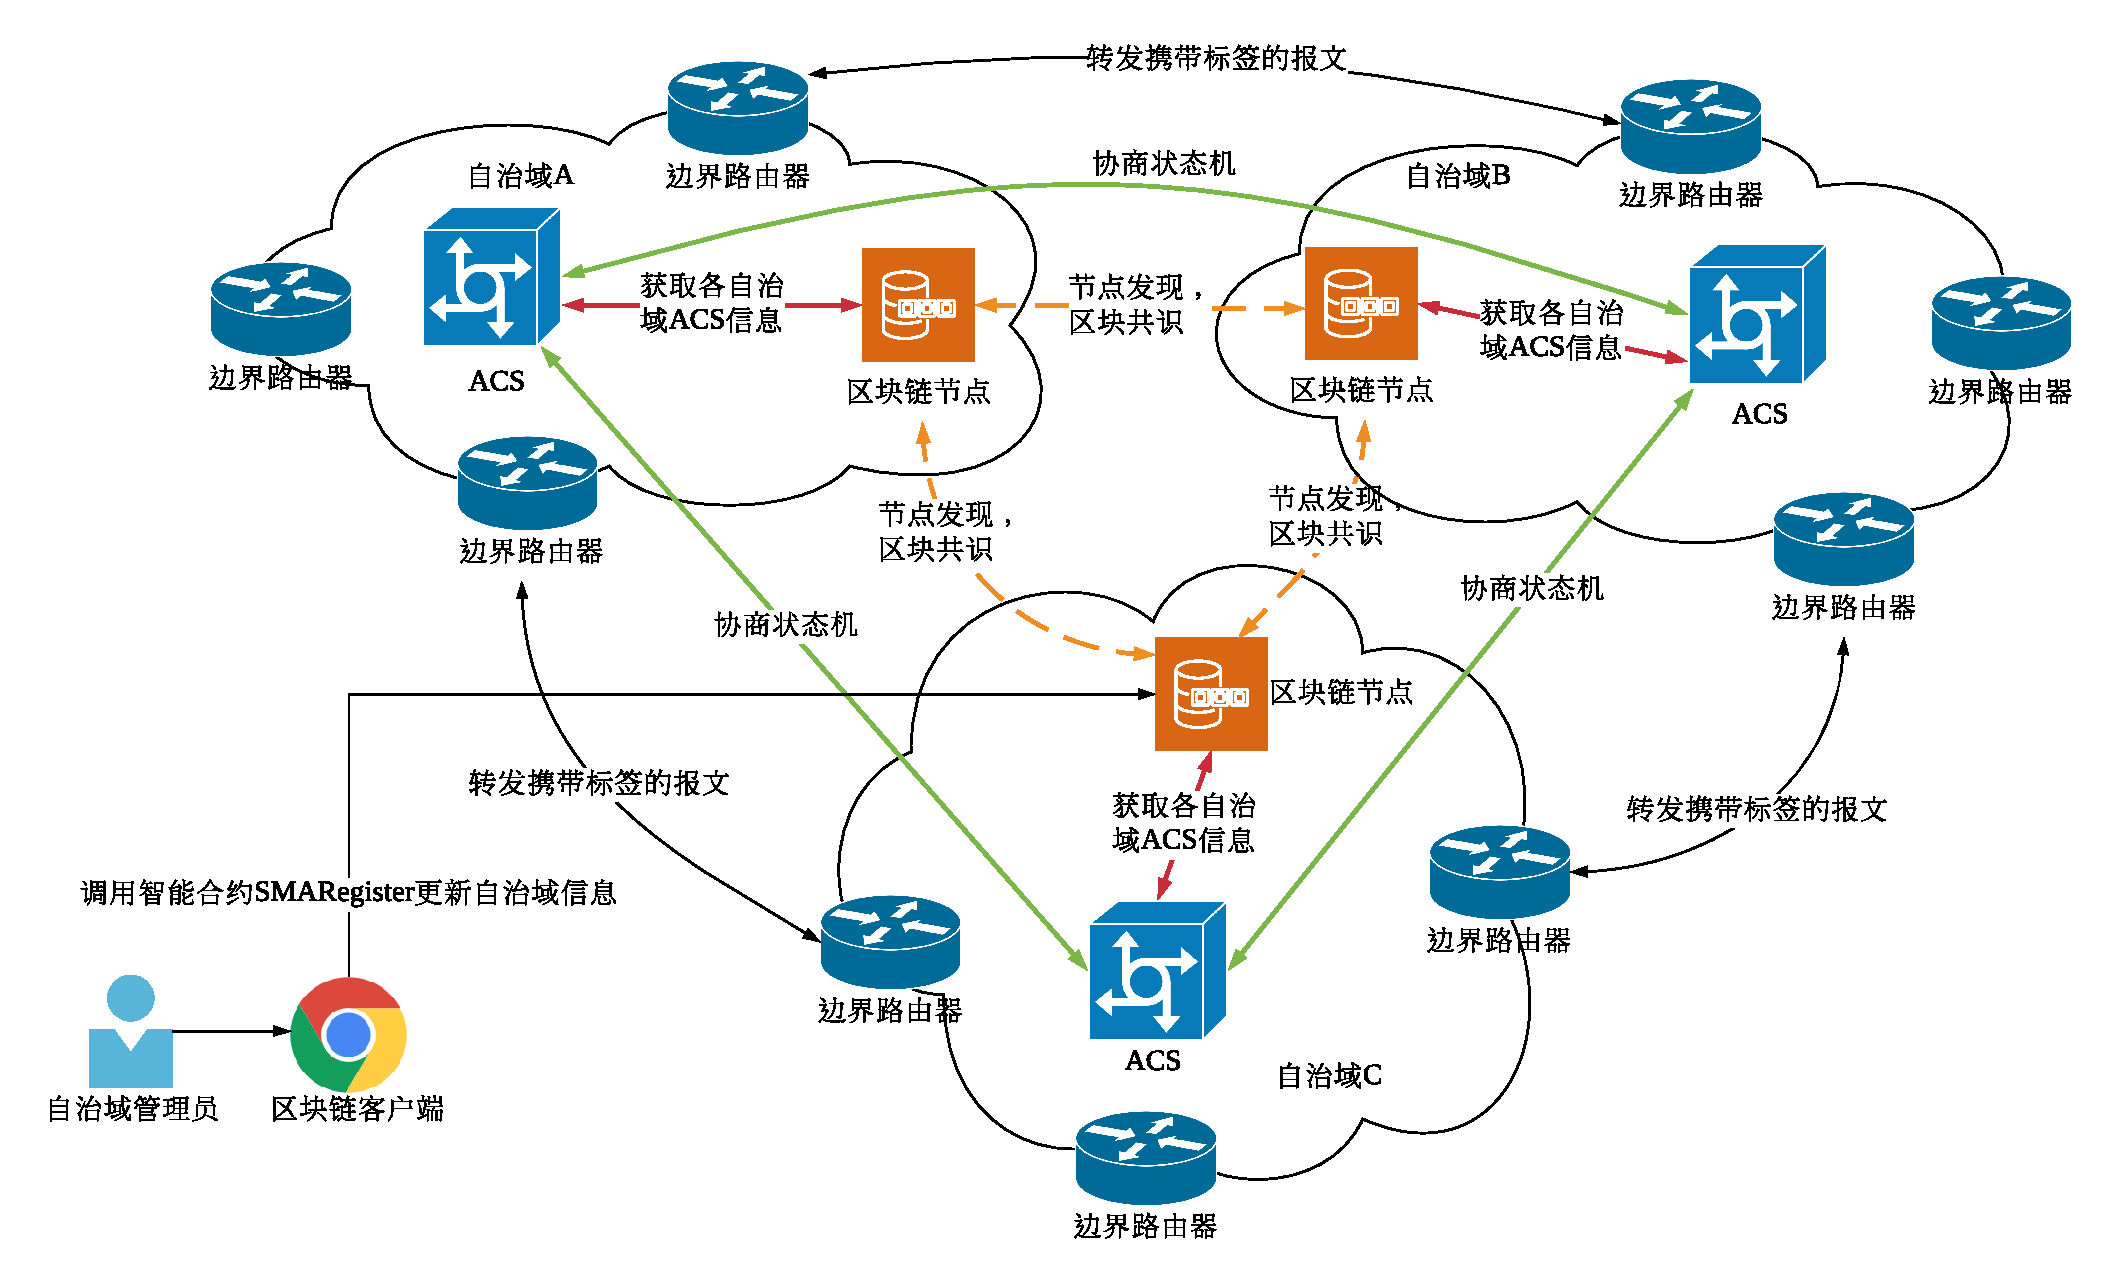
\includegraphics[width=\textwidth]{blockchain_sma_register_architecture.pdf}
        \caption{SMA联盟注册系统的区块链设计架构}
        \label{fig:blockchain_sma_register_architecture}
      \end{figure}

      在SMA原本的设计中,自治域信息更新采取部署SMA方案的自治域的管理员在线下向联盟管理员提交申请,联盟管理员审批后在REG服务器中进行手动维护的模式。本文将其变更为通过区块链提交申请,联盟管理员在链上对其申请进行审批的模式,从而规范化这一过程,并且保证自治域信息的更迭历史也可以得到保护和审计。
      此外,SMA采用REG定期向各ACS发送心跳以探测ACS状态并更新ACS信息列表,但采用区块链架构后由于区块链上的智能合约执行是一个多节点共识的过程,难以执行类似于单节点执行应用程序并通过API与外部系统进行交互的操作,因此本文设计了由ACS主动向联盟注册系统区块链定期拉取ACS信息列表的方式,将联盟注册信息的维护与更新两者解耦,由各自治域负责使用客户端向RegChain轮询最新的联盟ACS信息。

      本文设计了两个智能合约实现RegChain功能,分别命名为SMARegister与ASInfo。其中SMARegister由联盟管理员在启用联盟注册系统区块链第一个节点后进行部署,其所需要维护的内部状态如表\ref{tab:contract_SMARegister}所示。其中ASRequest为携带自治域信息的结构体,记录了自治域加入或离开安全联盟时提交申请的信息,包括申请类型、自治域号以及其他自治域相关信息等。ASInfo由SMARegister通过自治域申请时为自治域生成并部署,记录了特定自治域的信息以及ACS更新列表,其结构如表\ref{tab:contract_ASInfo}所示,其中AddrTime为一个包含ACS的IPv6地址与生效时间的二元组,类型为(String, Integer)。

      \begin{table}[htb]
        \centering
        \begin{minipage}[t]{\linewidth} 
          \caption{合约SMARegister信息列表}
          \label{tab:contract_SMARegister}
          \begin{tabularx}{\linewidth}{>{\centering\arraybackslash}X>{\centering\arraybackslash}X>{\centering\arraybackslash}X}
            \toprule[1.5pt]
            {\heiti 属性名} & {\heiti 类型} & {\heiti 说明} \\\midrule[1pt]
            req\_queue & ASRequest Array & 待审批的自治域信息更新请求列表 \\ 
            as\_queue & ASInfo Array & 自治域合约列表 \\
            \bottomrule[1.5pt]
          \end{tabularx}
        \end{minipage}
      \end{table}
      
      \begin{table}[htb]
        \centering
        \begin{minipage}[t]{\linewidth} 
          \caption{合约ASInfo信息列表}
          \label{tab:contract_ASInfo}
          \begin{tabularx}{\linewidth}{>{\centering\arraybackslash}X>{\centering\arraybackslash}X>{\centering\arraybackslash}X}
            \toprule[1.5pt]
            {\heiti 属性名} & {\heiti 类型} & {\heiti 说明} \\\midrule[1pt]
            id & String & 唯一标识自治域的标识符 \\ 
            asn & Integer & 自治域号 \\
            name & String & 自治域名 \\
            description & String & 自治域详细信息 \\
            acs\_queue & AddrTime Array & 自治域ACS信息列表 \\
            \bottomrule[1.5pt]
          \end{tabularx}
        \end{minipage}
      \end{table}

      本文在尽可能与原协议设计保持一致的情况下,设计各功能基于区块链的实现如下,均由SMARegister与ASInfo合约提供函数给各自治域管理员与ACS进行调用:
      \begin{enumerate}[1{)}]
        \item \textbf{自治域申请}:在自治域加入或离开SMA安全联盟时,填写自治域相关信息,包括申请类型、自治域号、自治域名称、详细信息,签发交易调用SMARegister的自治域申请函数,由SMARegister将其加入req\_queue中,等待联盟管理员审核。联盟管理员可通过SMARegister提供的查询函数查看已有的申请,当需要批准或拒绝申请时,其使用联盟管理的私钥签发交易调用SMARegister的函数进行批准或拒绝。审批通过的自治域将生成一个新的ASInfo合约加入as\_queue中并部署在区块链上,为该自治域提供ACS更新服务。
        \item \textbf{自治域ACS更新}:自治域管理员填写ACS的IPv6地址、配置生效时间等信息,使用自治域私钥签发交易广播给RegChain网络,交易中包含对其管理的ASInfo合约提供的自治域ACS更新函数的调用。ACS更新的操作将自动执行,不需要等待联盟管理员的审批,从而增加SMA控制平面信息更新的便捷性。
        \item \textbf{ACS信息同步}:ACS信息的定期同步功能由REG移交到各自治域的ACS,ACS周期性调用SMARegister提供的查询接口,更新本地的联盟ACS信息列表。由于仅对数据进行查询,不需要向区块链中写入新数据,因此ACS信息同步可以即时完成,不需要等待区块链的下一次出块。
      \end{enumerate}

      \subsubsection{自治域申请审批机制}
      \label{IPv6_Security:interas:design:update}
      自治域申请发生在有新的自治域部署SMA方案或已部署的自治域离开SMA安全联盟时,本文设计自治域申请的格式如表\ref{tab:blockchain_design_as_request}所示,将其称为ASRequest。
      \begin{table}[htb]
        \centering
        \begin{minipage}[t]{\linewidth} 
          \caption{自治域申请ASRequest格式}
          \label{tab:blockchain_design_as_request}
          \begin{tabularx}{\linewidth}{cc>{\centering\arraybackslash}X>{\centering\arraybackslash}X}
            \toprule[1.5pt]
            {\heiti 名称} & {\heiti 类型} & {\heiti 举例} & {\heiti 说明} \\\midrule[1pt]
            req\_type & Enum & Register & 指示自治域申请类型的枚举,包含Register与Delete  \\ 
            asn & Integer & 45576 & 自治域号 \\
            name & String & CERNET2-TSINGHUA6-AS-AP & 自治域名称 \\
            description & String & Tsinghua University & 自治域的详细信息 \\
            \bottomrule[1.5pt]
          \end{tabularx}
        \end{minipage}
      \end{table}

      其中,req\_type用于指示本次申请的类型,分为Register与Delete两种。为了便于自治域信息的查找与更新权限控制,在自治域注册申请被联盟管理员批准后,SMARegister将为其部署一个新的ASInfo合约,以该次交易的钱包地址作为所有者,与该自治域的AS号进行绑定,后续对合约进行更新的交易必须由同一地址的账户发起。

      自治域管理员填写自治域申请后,经由客户端签发交易并广播,调用智能合约SMARegister提供的自治域申请函数,本文将其命名为createASRequest。RegChain中的节点收到该交易后进行共识,调用各自维护的SMARegister执行相关调用。createASRequest将自治域申请加入到req\_queue中等待联盟管理员审批,并不直接更新as\_queue队列。联盟管理员通过调用SMARegister的requestQuery接口查看待审批列表,对自治域申请进行审批,分别调用SMARegister的requestApprove与requestReject函数进行批准或拒绝。经过批准的自治域信息将被用于生成一个新的ASInfo合约,并加入到as\_queue中。自治域申请与审批的时序如图\ref{fig:blockchain_as_update_procedure}所示。
      
      \begin{figure}[ht]
        \centering
        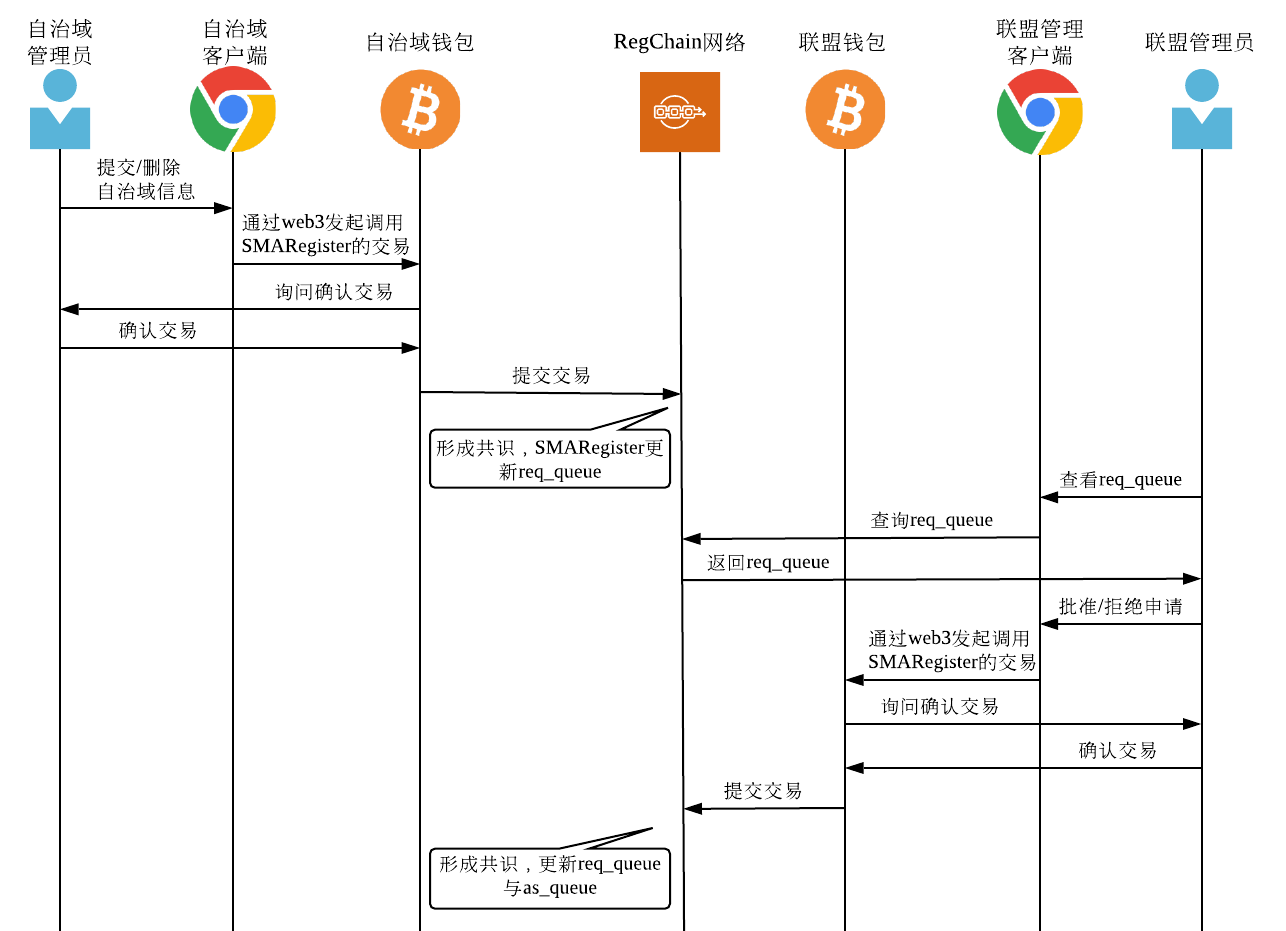
\includegraphics[width=\textwidth]{blockchain_as_update_procedure.png}
        \caption{RegChain自治域申请时序}
        \label{fig:blockchain_as_update_procedure}
      \end{figure}

      SMARegister为自治域申请审批机制提供的相关函数总结如表\ref{tab:contract_as_request_function}所示。

      \begin{table}[htb]
        \centering
        \begin{minipage}[t]{\linewidth} 
          \caption{SMARegister自治域申请审批相关函数}
          \label{tab:contract_as_request_function}
          \begin{tabularx}{\linewidth}{cccc>{\centering\arraybackslash}X}
            \toprule[1.5pt]
            {\heiti 函数名} & {\heiti 参数类型} & {\heiti 返回类型} & {\heiti 调用者} & {\heiti 说明} \\\midrule[1pt]
            createASRequest & ASRequest & 无 & 自治域管理员 & 提交自治域申请 \\ 
            requestQuery & 无 & ASRequest Array & 联盟管理员 & 查看待审批的自治域申请列表 \\ 
            requestApprove & String & 无 & 联盟管理员 & 接收自治域标识,通过其对应AS的申请 \\ 
            requestReject & String & 无 & 联盟管理员 & 接收自治域标识,拒绝其对应AS的申请 \\ 
            \bottomrule[1.5pt]
          \end{tabularx}
        \end{minipage}
      \end{table}

      \subsubsection{自治域ACS更新机制}
      在自治域申请经过联盟管理员批准后,该自治域将拥有一个独立的ASInfo合约记录其信息并提供ACS更新服务。自治域管理员可通过其申请时的钱包地址自主调用updateACS函数进行ACS配置的更新,而无需调用SMARegister要求联盟管理员的批准。

      由于自治域ACS信息并不即时生效,可能在将来某个时间点才发生切换,因此ASInfo必须将ACS的历次更新均记录下来,以供后续配置的平滑切换,而不是简单地记录一个ACS的最新信息,因此表\ref{tab:contract_ASInfo}中使用了acs\_queue对其进行记录。当有新的ACS配置更新时,先前生效时间晚于其生效时间的ACS配置将自动失效,其更新算法如算法\ref{algo:blockchain_as_update}所示。

      \begin{algorithm}
        \caption{RegChain自治域ACS更新算法}
        \label{algo:blockchain_as_update}
        
        \LinesNumbered
        \SetKw{KwInList}{in}
        \SetKw{KwDownto}{downto}

        \SetKw{KwBreak}{break}
        \SetKw{KwReturn}{return}
        
        \SetKw{KwTrue}{true}
        \SetKw{KwFalse}{false}
        
        \SetKw{KwAnd}{and}
        \SetKw{KwNot}{not}
        
        \SetKw{KwAssert}{assert}
        \SetKw{KwNew}{new}


        \KwIn{acs\_addr, effect\_time}

        new\_pair \gets \KwNew AddrTime(acs\_addr, effect\_time)\;
        \While{as\_info.acs\_queue.length() > 0} {
            last\_time \gets as\_info.acs\_queue.lastElement().effect\_time\;
            \If{effect\_time <= last\_time} {
                as\_info.acs\_queue.removeLastElement()\;
            }
            \Else {
                \KwBreak\;
            }
        }
        as\_info.acs\_queue.add(new\_pair)\;
      \end{algorithm}


      \subsubsection{ACS信息同步机制}
      \label{IPv6_Security:interas:design:heartbeat}
      ACS信息同步机制由原先的REG主动推送修改为ACS主动查询。由于ACS向RegChain查询联盟ACS信息列表不需要向区块链中写入数据,因此其是一个即时操作,不需要各节点达成共识。本文设计SMARegister提供联盟内所有自治域的ASInfo列表查询函数ASQuery,并设计ASInfo合约提供查询该自治域当前有效ACS地址的函数getCurrentACS,两者如表\ref{tab:contract_as_query_function}所示。客户端进行ACS信息拉取时,首先向SMARegister获取所有自治域的ASInfo合约,然后分别对每个自治域进行当前ACS地址的获取。
      \begin{table}[htb]
        \centering
        \begin{minipage}[t]{\linewidth} 
          \caption{自治域信息查询相关函数}
          \label{tab:contract_as_query_function}
          \begin{tabularx}{\linewidth}{cccc>{\centering\arraybackslash}X}
            \toprule[1.5pt]
            {\heiti 合约名} & {\heiti 函数名} & {\heiti 参数类型} & {\heiti 返回类型} & {\heiti 说明} \\\midrule[1pt]
            SMARegister & ASQuery & 无 & ASInfo Array & 获取联盟内所有自治域的ASInfo合约 \\ 
            ASInfo & getCurrentACS & Integer & String & 提交当前查询时间,获取当前有效的ACS地址 \\ 
            \bottomrule[1.5pt]
          \end{tabularx}
        \end{minipage}
      \end{table}

      之所以要在getCurrentACS的参数中携带查询时的时间信息,是由于在EVM内部无法获知当前的确切时间,因此需要ACS主动将当前时间告知ASInfo,这一步骤由RegChain的客户端自动填充,不需要手动填写。ASInfo将根据查询时间,对维护的ACS信息列表进行从头到尾的扫描,以确定在该时间点生效的ACS信息,由于这一算法较为简单,故不再赘述。

    \subsection{基于以太坊的SMA联盟注册系统实现}
    \label{IPv6_Security:interas:implement}
    SMA联盟注册系统的主要功能是自治域信息的更新与查询,由于现实网络中为了维持域间报文转发的稳定,自治域管理员并不会频繁更新自治域ACS的地址,且其更新操作中携带有配置的生效时间,一般发生在未来若干小时甚至若干天后,因此对于更新的实时性没有特别高的要求。查询操作要求很高的实时性,但由于其不需要向区块链中写入数据,因此可以实时返回结果,与区块链采用的共识算法无关。另一方面,倘若采用Raft等共识算法,虽然可以提高共识效率,但却以牺牲对恶意节点接入的防御能力为代价,从而使SMA联盟注册系统的安全性大打折扣。综上考虑,本文选择PoW作为共识算法,采用以太坊平台实现RegChain,项目代码参见RegChain的Git仓库\footnote{RegChain repository, https://github.com/BragCat/RegChain}。

      \subsubsection{整体架构}
      \label{IPv6_Security:interas:implement:architecture}
      为了实现对用户的友好,本文的客户端采用React\footnote{React, https://zh-hans.reactjs.org/docs/getting-started.html}开发,自治域管理员只需要使用浏览器并安装一个钱包插件即可使用,而无需安装特殊的客户端。希望能够参与网络共识的自治域,可以在本地部署一个以太坊节点,以更稳定地提供共识与接入服务,以太坊节点可选择Parity\footnote{Parity, https://www.parity.io/ethereum/}、Geth\footnote{Geth, https://geth.ethereum.org/}等任意一款支持运行完整以太坊节点的软件。客户端通过Web3.js\footnote{Web3, https://github.com/ethereum/wiki/wiki/JavaScript-API}连接到区块链节点进行数据的读写,其架构方式与传统网络应用的对比如图\ref{fig:blockchain_tradition_ethereum_comparison}所示,在以太坊构建的应用中,Web3.js相当于传统应用中的后端,本文将使用Web3.js的API开发相应的逻辑进行连接区块链节点、构建交易、读写区块链数据等交互操作。区块链网络相当于传统应用中对应的数据库,但其提供了更高的可用性与更加强大的安全特性。

      \begin{figure}[ht]
        \centering
        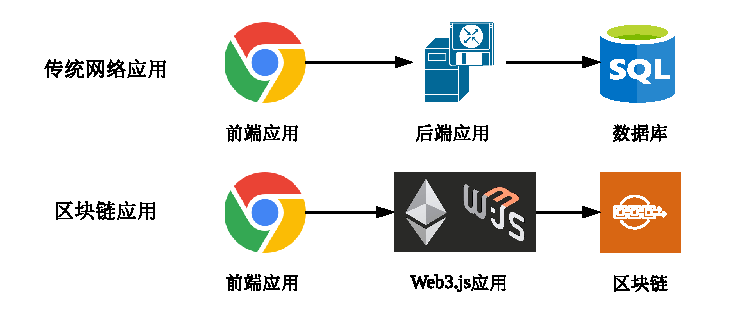
\includegraphics[width=0.8\textwidth]{blockchain_tradition_ethereum_comparison.pdf}
        \caption{传统网络应用与以太坊应用架构对比}
        \label{fig:blockchain_tradition_ethereum_comparison}
      \end{figure}

      RegChain的以太坊实现包含图\ref{fig:blockchain_regchain_implementation}所示的两个部分,一部分为使用React框架开发的网页客户端,主要包括联盟管理员查看与审批申请、自治域管理员提交请求等功能,自治域管理员与联盟管理员只需要在Chrome浏览器或Firefox浏览器上安装支持以太坊的钱包插件,如MetaMask,即可使用浏览器访问React App提供的页面并进行操作;另一部分为将自治域信息查询功能封装后的Javascript包,提供联盟内ACS信息的拉取服务,其内部调用Web3.js与区块链进行交互,向外提供查询自治域ACS信息的接口,自治域ACS调用其接口即可向区块链查询获得联盟内所有自治域当前有效的ACS地址。两个部分共享同一个后端服务,即RegChain区块链上的智能合约SMARegister与各个自治域对应的ASInfo。
      
      \begin{figure}[ht]
        \centering
        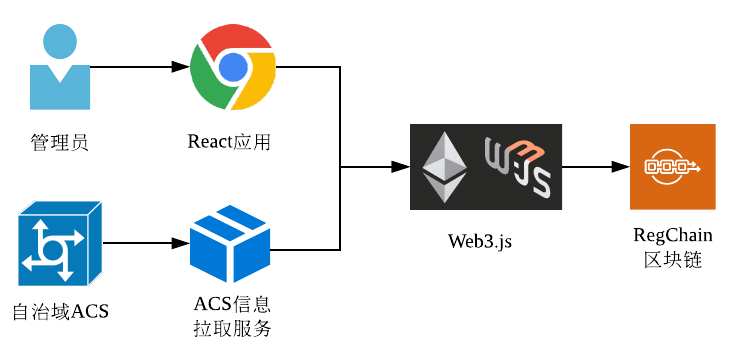
\includegraphics[width=0.8\textwidth]{figures/blockchain_regchain_implementation.png}
        \caption{SMA联盟注册系统的以太坊实现架构}
        \label{fig:blockchain_regchain_implementation}
      \end{figure}

      \subsubsection{DApp}
      \label{IPv6_Security:interas:implement:dapp}
      DApp是具有执行能力的应用代码,其以智能合约的形式部署在每一个以太坊节点上,每个节点对于新区块中的交易,依次执行智能合约的调用,各自独立维护合约内部状态。由于所有执行步骤的确定性,最终每个以太坊节点上合约状态都将保持一致,相当于同一个应用分布在整个网络的节点上执行,保持了应用的多个副本,因此被称为分布式应用。本文采用Truffle\footnote{Truffle, https://www.trufflesuite.com/docs}工具链开发与测试DApp。
      
      SMA联盟注册系统的DApp主要需要实现智能合约SMARegister与ASInfo,两者需要维护的内部状态已由表\ref{tab:contract_SMARegister}与表\ref{tab:contract_ASInfo}定义,本文在使用Solidity进行实现时,由于Solidity语言的一些限制,因此与原设计有所区别。
      SMARegister中两个数组即对应了Solidity中的动态数组类型,但对ASRequest结构体做了一些更改,如表\ref{tab:ethereum_ASRequest_attributes}所示。ASInfo中各属性除ACS列表外均由ASRequest生成,在此不再赘述。
      \begin{table}[htb]
        \centering
        \begin{minipage}[t]{\linewidth} 
          \caption{ASRequest数据结构}
          \label{tab:ethereum_ASRequest_attributes}
          \begin{tabularx}{\linewidth}{cc>{\centering\arraybackslash}X>{\centering\arraybackslash}X}
            \toprule[1.5pt]
            {\heiti 属性名} & {\heiti 原类型} & {\heiti Solidity数据结构} & {\heiti 说明} \\\midrule[1pt]
            owner & 未定义 & address & 发起申请交易的钱包地址 \\
            id & String & bytes20 & 根据owner生成的自治域标识 \\
            req\_type & Enum & uint256 & 0表示Register,1表示Delete \\ 
            asn & Integer & uint256 & 自治域号 \\
            name & String & string & 自治域名 \\
            description & String & string & 自治域详细信息 \\
            \bottomrule[1.5pt]
          \end{tabularx}
        \end{minipage}
      \end{table}

      之所以需要将自治域标识id与ASInfo的所有者owner进行分别存储,是由于Javascript没有Solidity的address所对应的类型,在客户端通过自治域标识进行对应自治域申请审批时无法直接发送address类型的数据,因此只能使用字符串存储id以与客户端兼容。同时,由于Solidity暂时不支持返回结构体数组,比如string[],因此必须将id定义为bytes20而非变长的string类型以支持requestQuery函数查询当前所有的自治域申请。

      SMARegister与ASInfo实现了\ref{IPv6_Security:interas:design}节中提到的各函数,并采用了modifier对函数调用者身份进行限定,仅允许SMARegister的部署者即联盟管理员调用requestApprove与requestReject函数,仅允许ASInfo的所有者调用updateACS函数。
    
      图\ref{fig:regchain_dapp_tx}展示了RegChain在实验中的一些交易历史,从头至尾查看历次交易即可获知RegChain所经历的所有历史状态。为了审计的便利性,本文在实现DApp时还利用以太坊的事件机制,设计了ASCreated、ASRequestApproved等多个事件,如图\ref{fig:regchain_dapp_event}所示,在RegChain网络执行合约时将根据交易的调用生成相应的事件形成日志,便于查看RegChain中各自治域的变更历史。

      \begin{figure}[H]
        \centering
        \subcaptionbox{RegChain交易历史\label{fig:regchain_dapp_tx}}
        {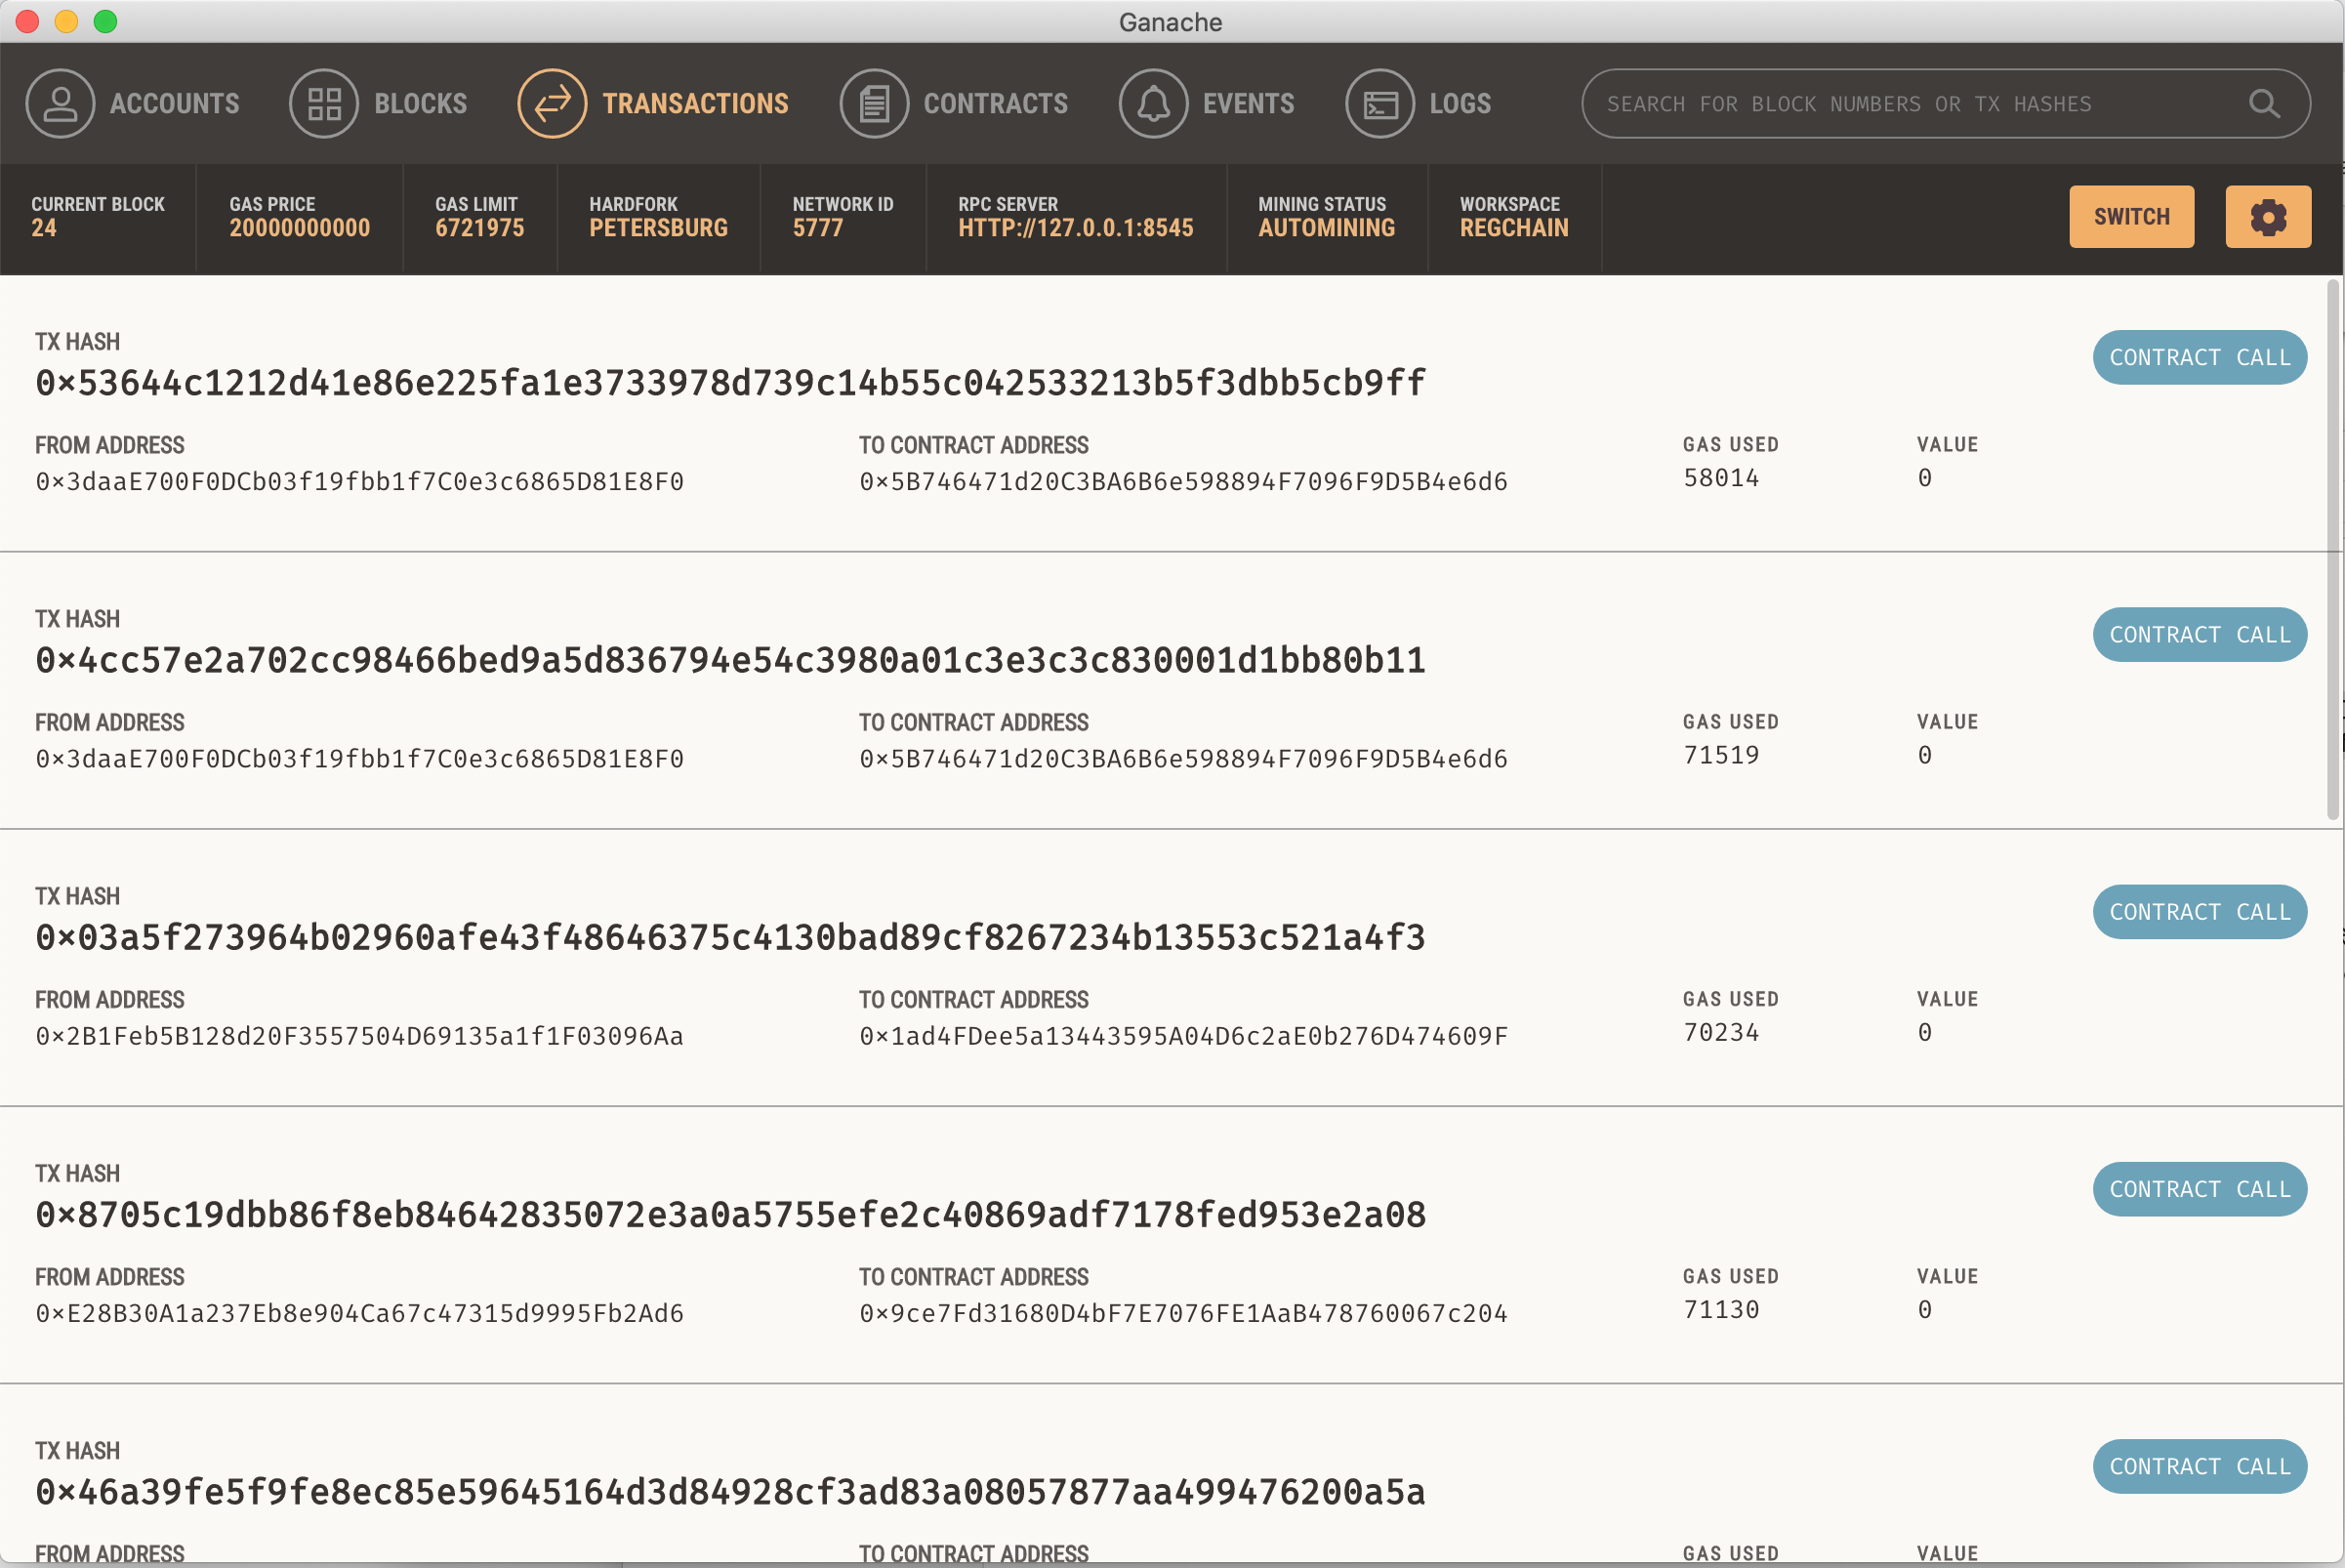
\includegraphics[height=4.8cm]{figures/regchain_dapp_tx.png}}
        \hspace{1em}
        \subcaptionbox{RegChain事件历史\label{fig:regchain_dapp_event}}
        {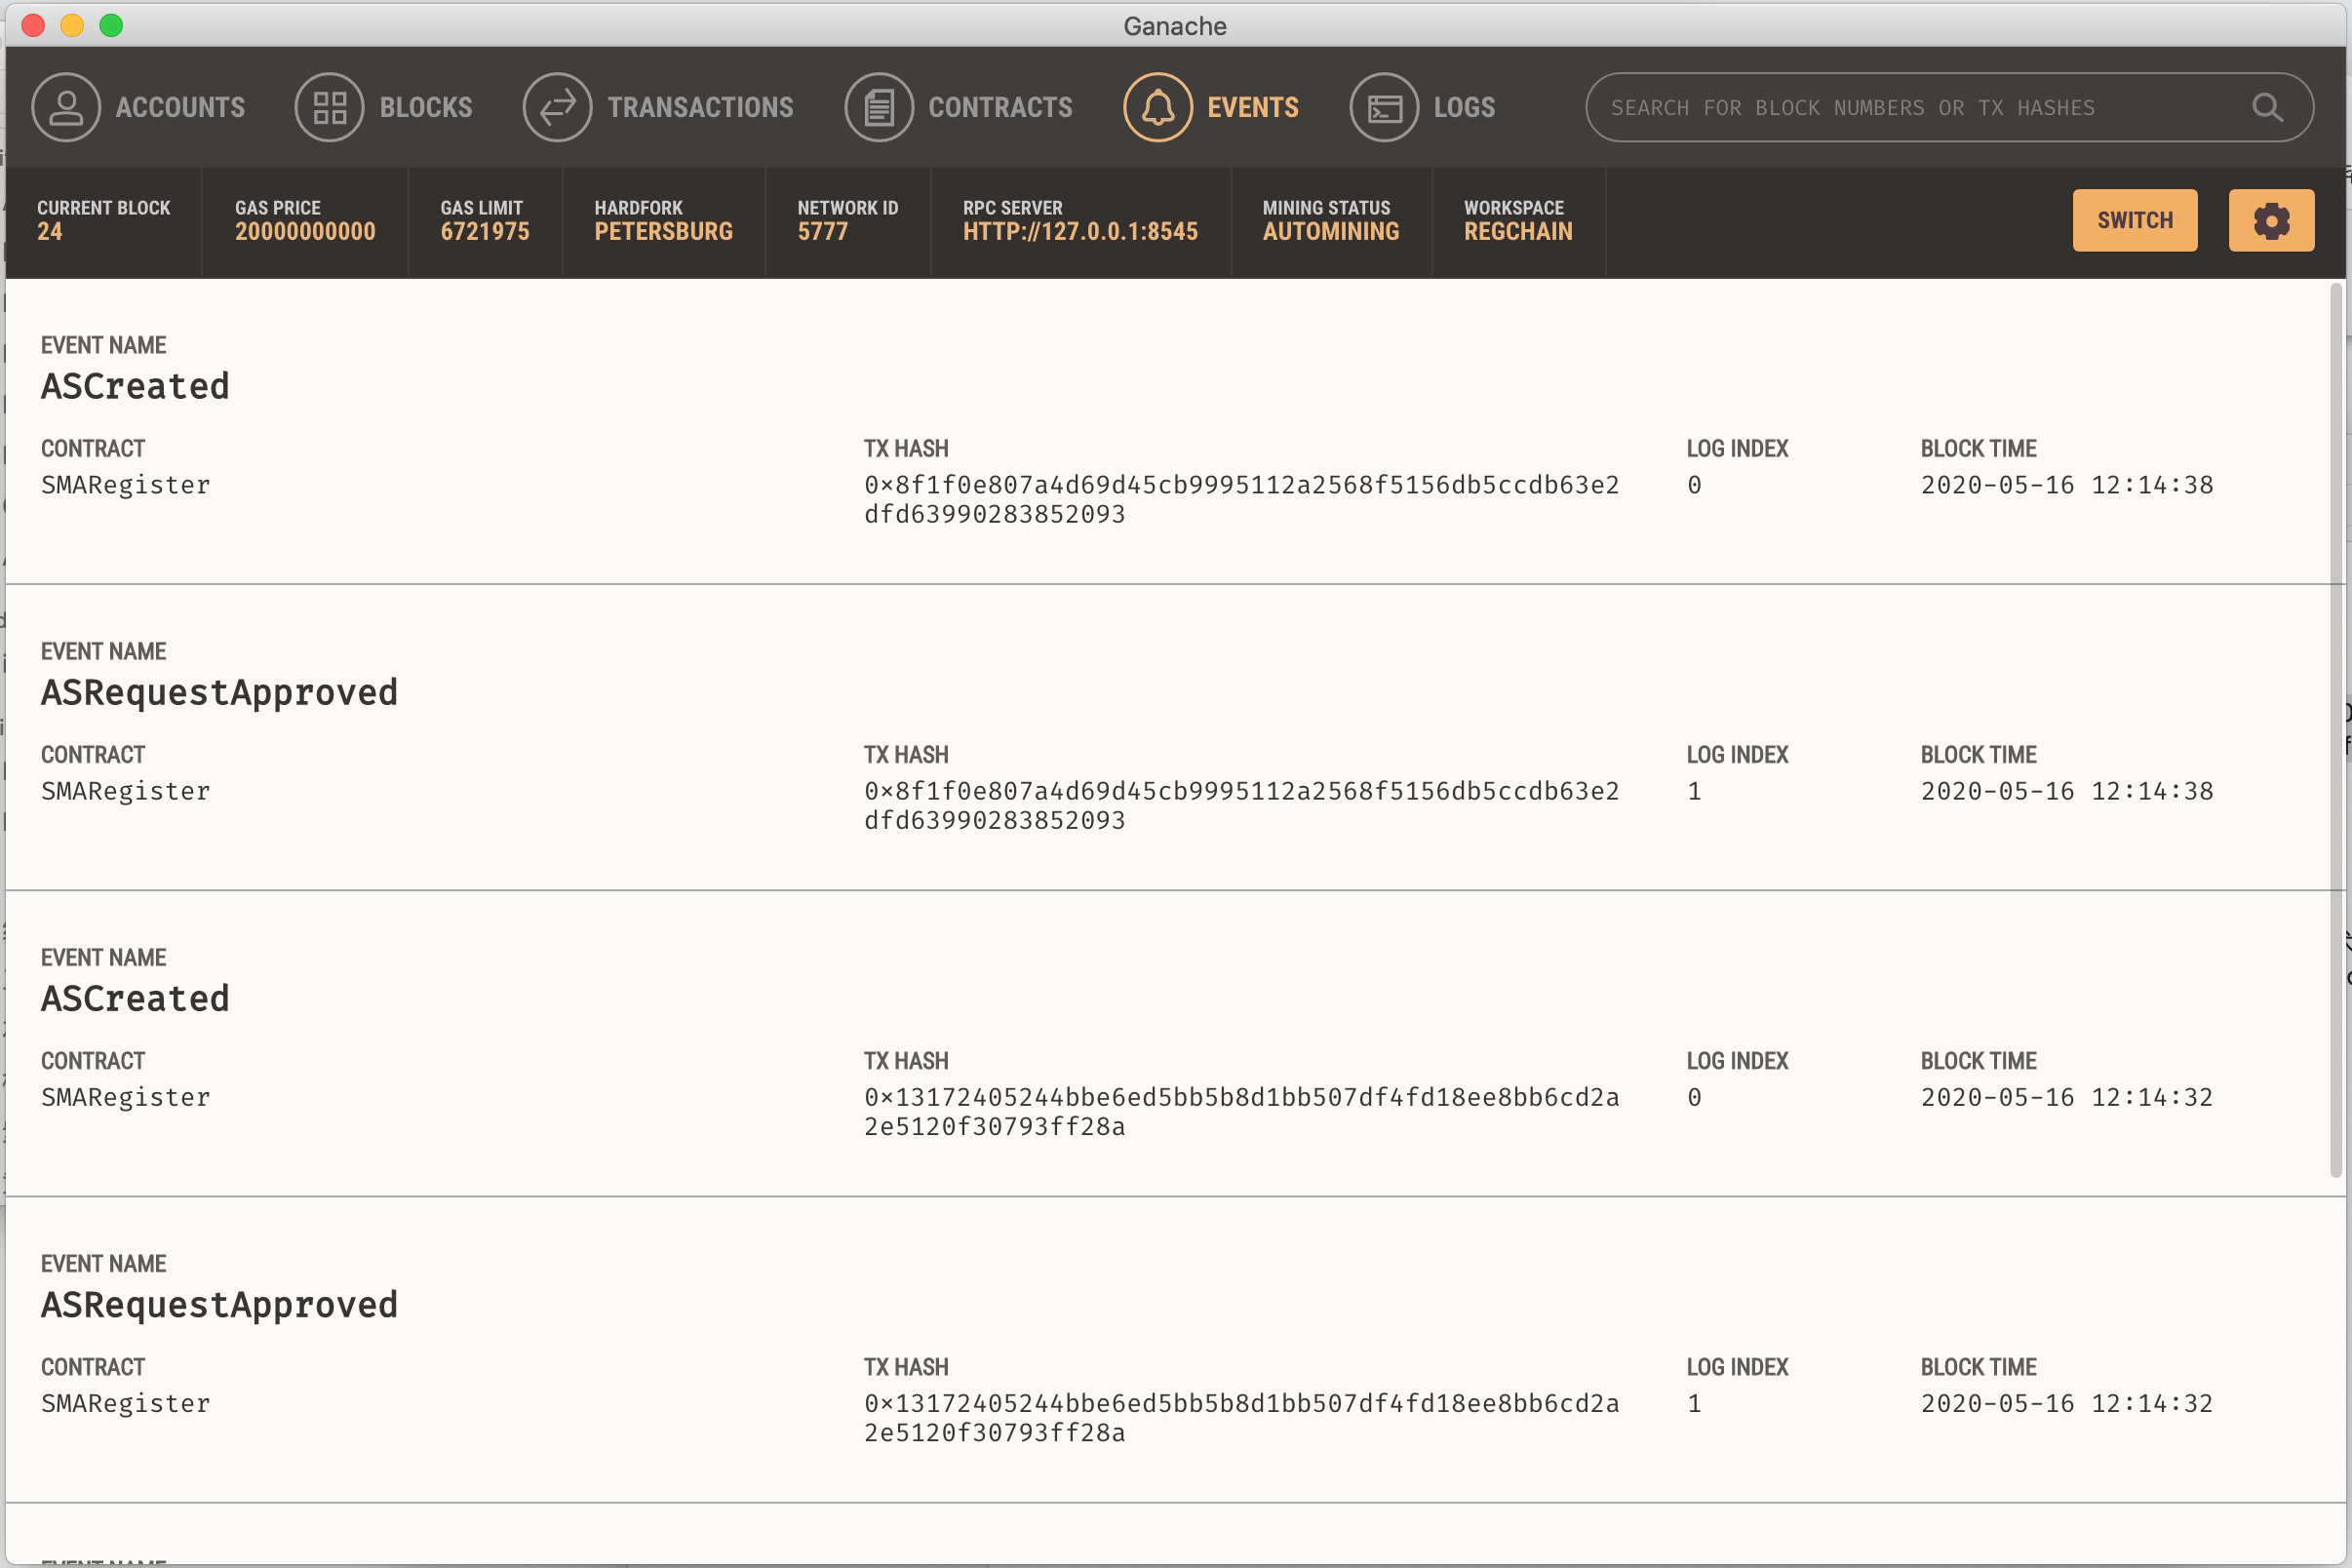
\includegraphics[height=4.8cm]{figures/regchain_dapp_event.png}}
        \caption{RegChain DApp端交易与事件展示}
        \label{fig:regchain_dapp_images}
      \end{figure}


      \subsubsection{客户端}
      \label{IPv6_Security:interas:implement:client}
      本文在客户端处的实现包含网页客户端与ACS信息拉取服务。
      
      网页客户端由React框架实现,提供自治域管理员与联盟管理员查看与操作RegChain的浏览器页面,两者的回调函数分别如表\ref{tab:sma_admin_client_callback_function}与表\ref{tab:sma_as_client_callback_function}所示。
      \begin{table}[htb]
        \centering
        \begin{minipage}[t]{\linewidth} 
          \caption{SMA联盟注册系统以太坊实现的联盟管理客户端回调函数}
          \label{tab:sma_admin_client_callback_function}
          \begin{tabularx}{\linewidth}{cc>{\centering\arraybackslash}X}
            \toprule[1.5pt]
            {\heiti 函数名} & {\heiti 参数名} & {\heiti 说明} \\\midrule[1pt]
            handleSubmitApprove & id & 联盟管理员点击自治域申请通过按钮的回调函数,调用SMARegister.requestApprove函数通过申请 \\ 
            handleSubmitReject & id & 联盟管理员点击自治域申请拒绝按钮的回调函数,调用SMARegister.requestReject函数拒绝申请 \\
            \bottomrule[1.5pt]
          \end{tabularx}
        \end{minipage}
      \end{table}
      
      \begin{table}[htb]
        \centering
        \begin{minipage}[t]{\linewidth} 
          \caption{SMA联盟注册系统以太坊实现的自治域客户端回调函数}
          \label{tab:sma_as_client_callback_function}
          \begin{tabularx}{\linewidth}{c>{\centering\arraybackslash}X>{\centering\arraybackslash}X}
            \toprule[1.5pt]
            {\heiti 函数名} & {\heiti 参数名} & {\heiti 说明} \\\midrule[1pt]
            handleSubmitRequest & req\_type, asn, name, description & 自治域管理员点击自治域申请提交按钮的回调函数,调用SMARegister.createASRequest提交申请 \\ 
            handleSubmitUpdate & acs\_addr, effect\_time & 自治域管理员点击自治域ACS更新提交按钮的回调函数,调用ASInfo.updateACS更新ACS配置 \\ 
            \bottomrule[1.5pt]
          \end{tabularx}
        \end{minipage}
      \end{table}


      
      自治域管理员进行自治域申请的页面如图\ref{fig:regchain_client_request}所示,可通过点击“自治域变更”进行自治域信息的填写。当自治域管理员点击提交按钮时,MetaMask将弹出询问是否允许使用当前账户进行交易签名。
      
      \begin{figure}[H]
        \centering
        \subcaptionbox{申请填写与提交\label{fig:regchain_client_request_1}}
        {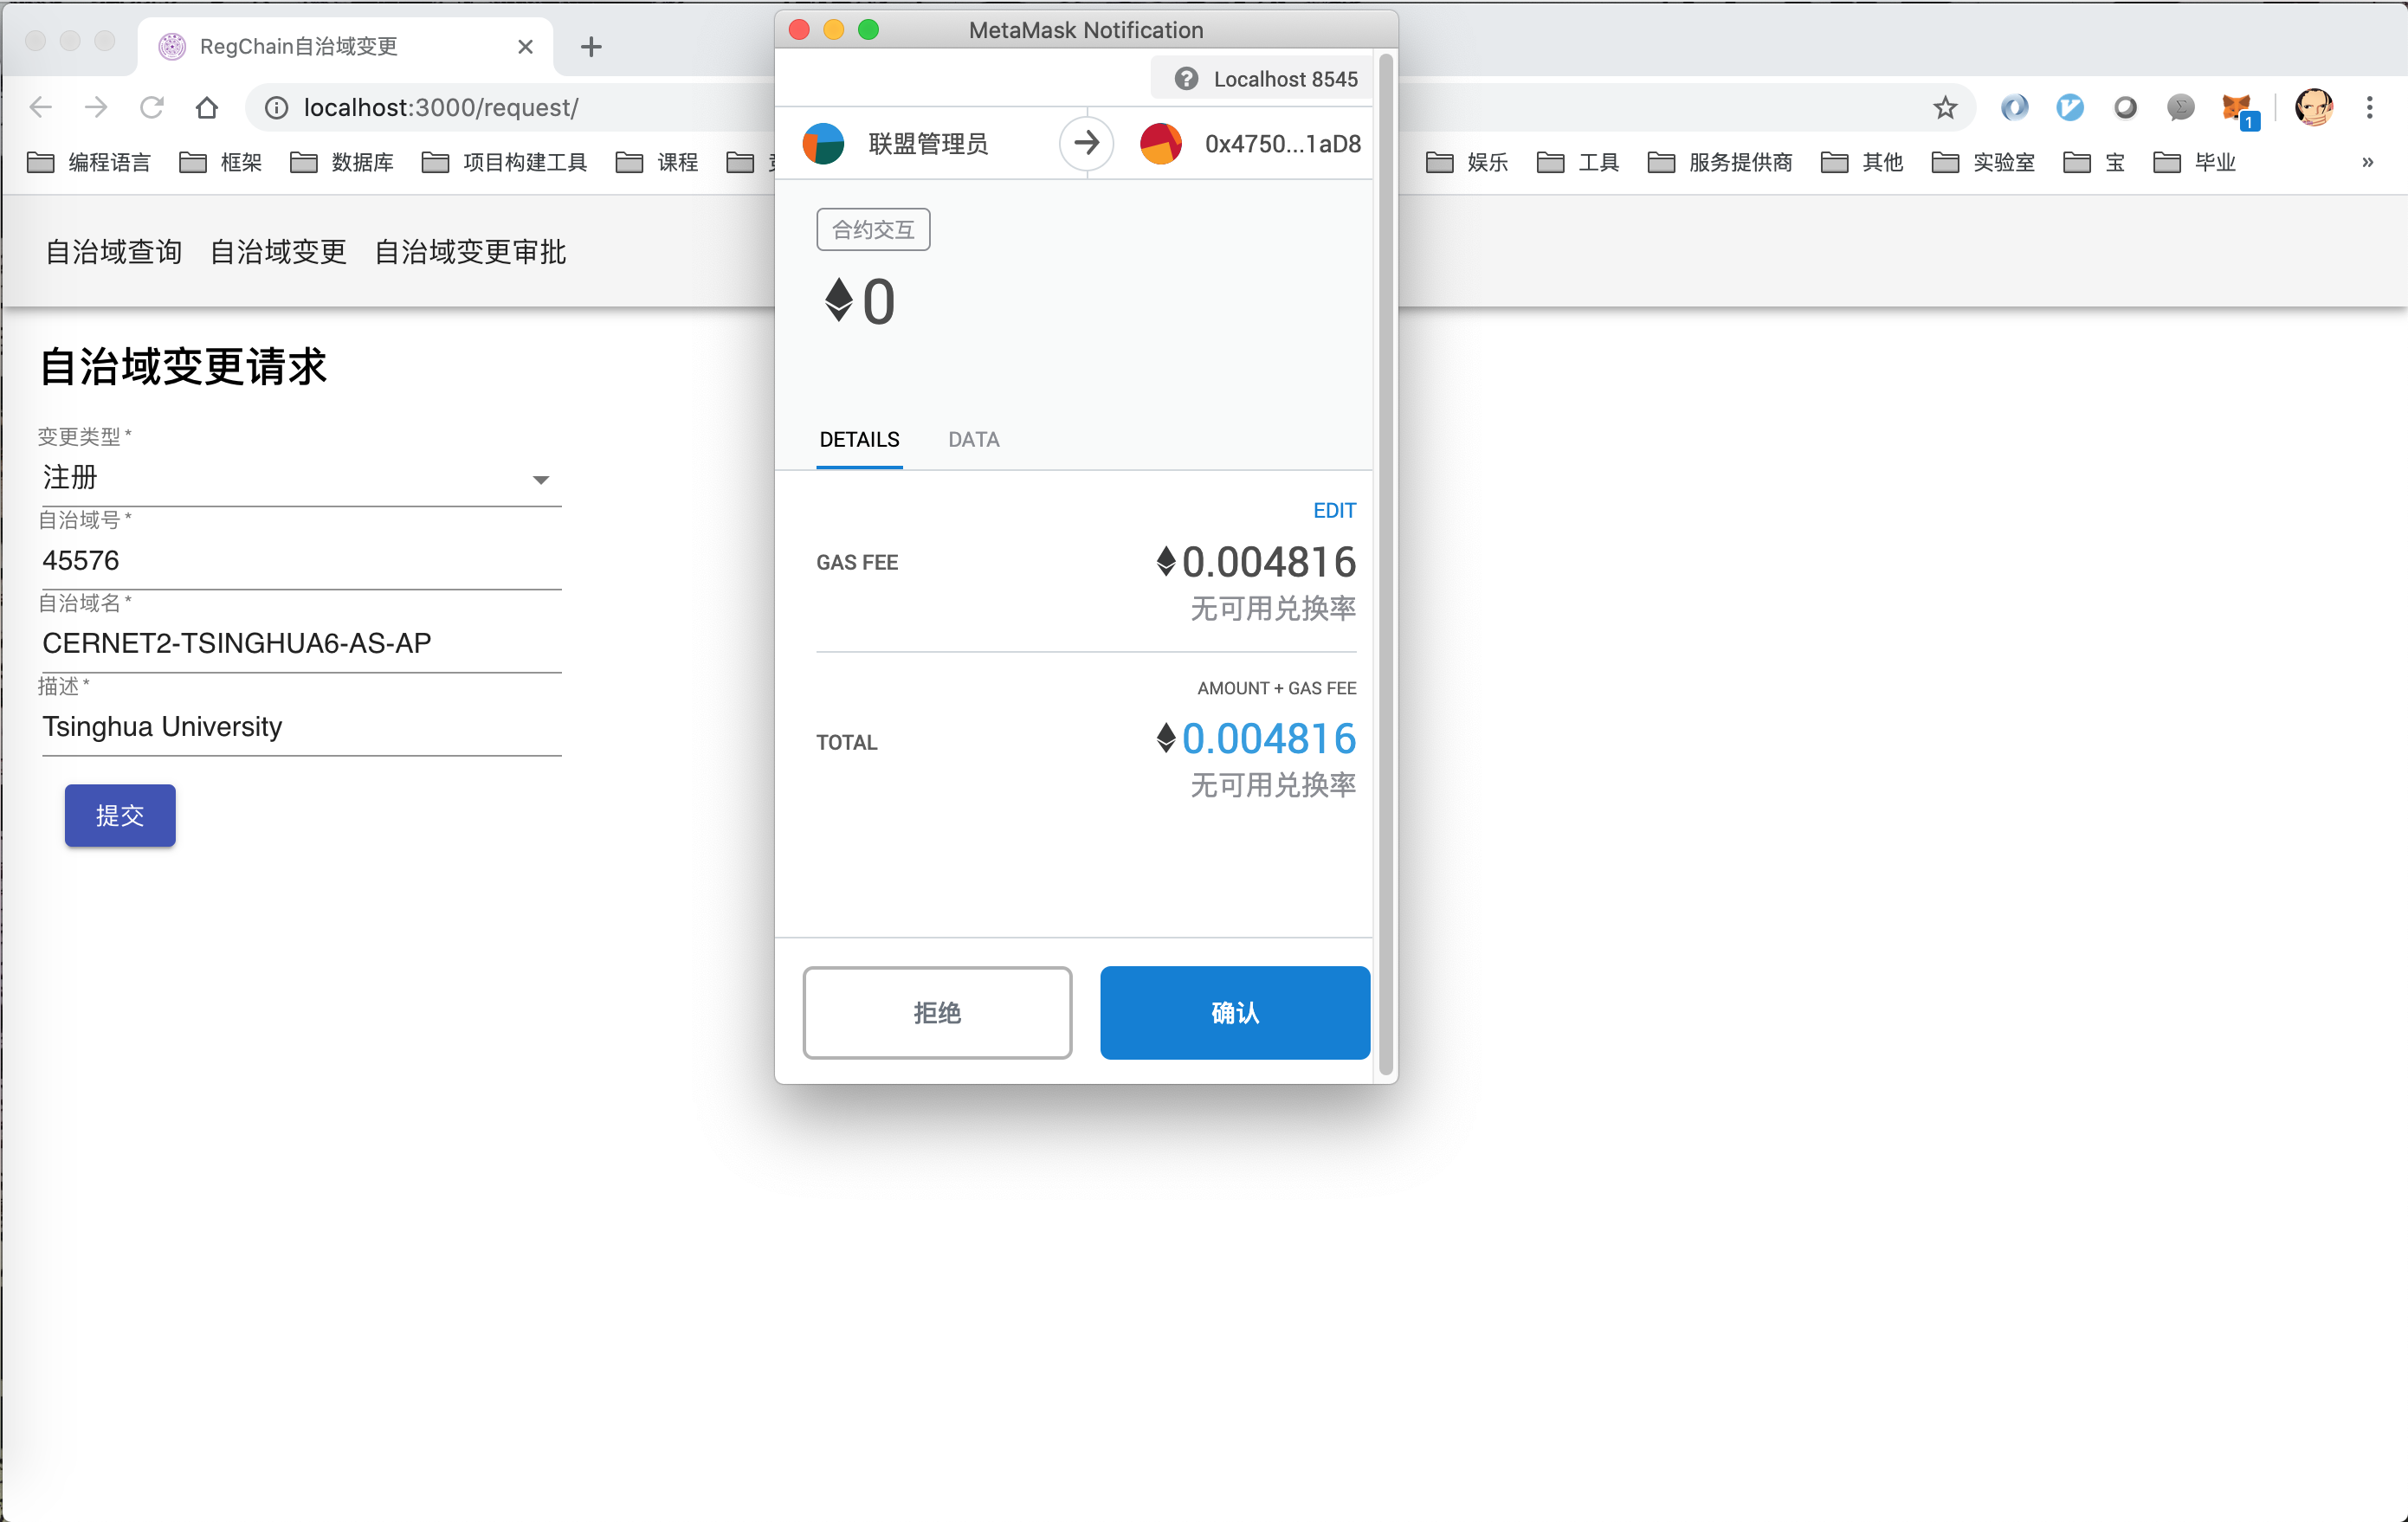
\includegraphics[height=4.5cm]{figures/regchain_client_request_1.png}}
        \hspace{1em}
        \subcaptionbox{申请提交成功\label{fig:regchain_client_request_2}}
        {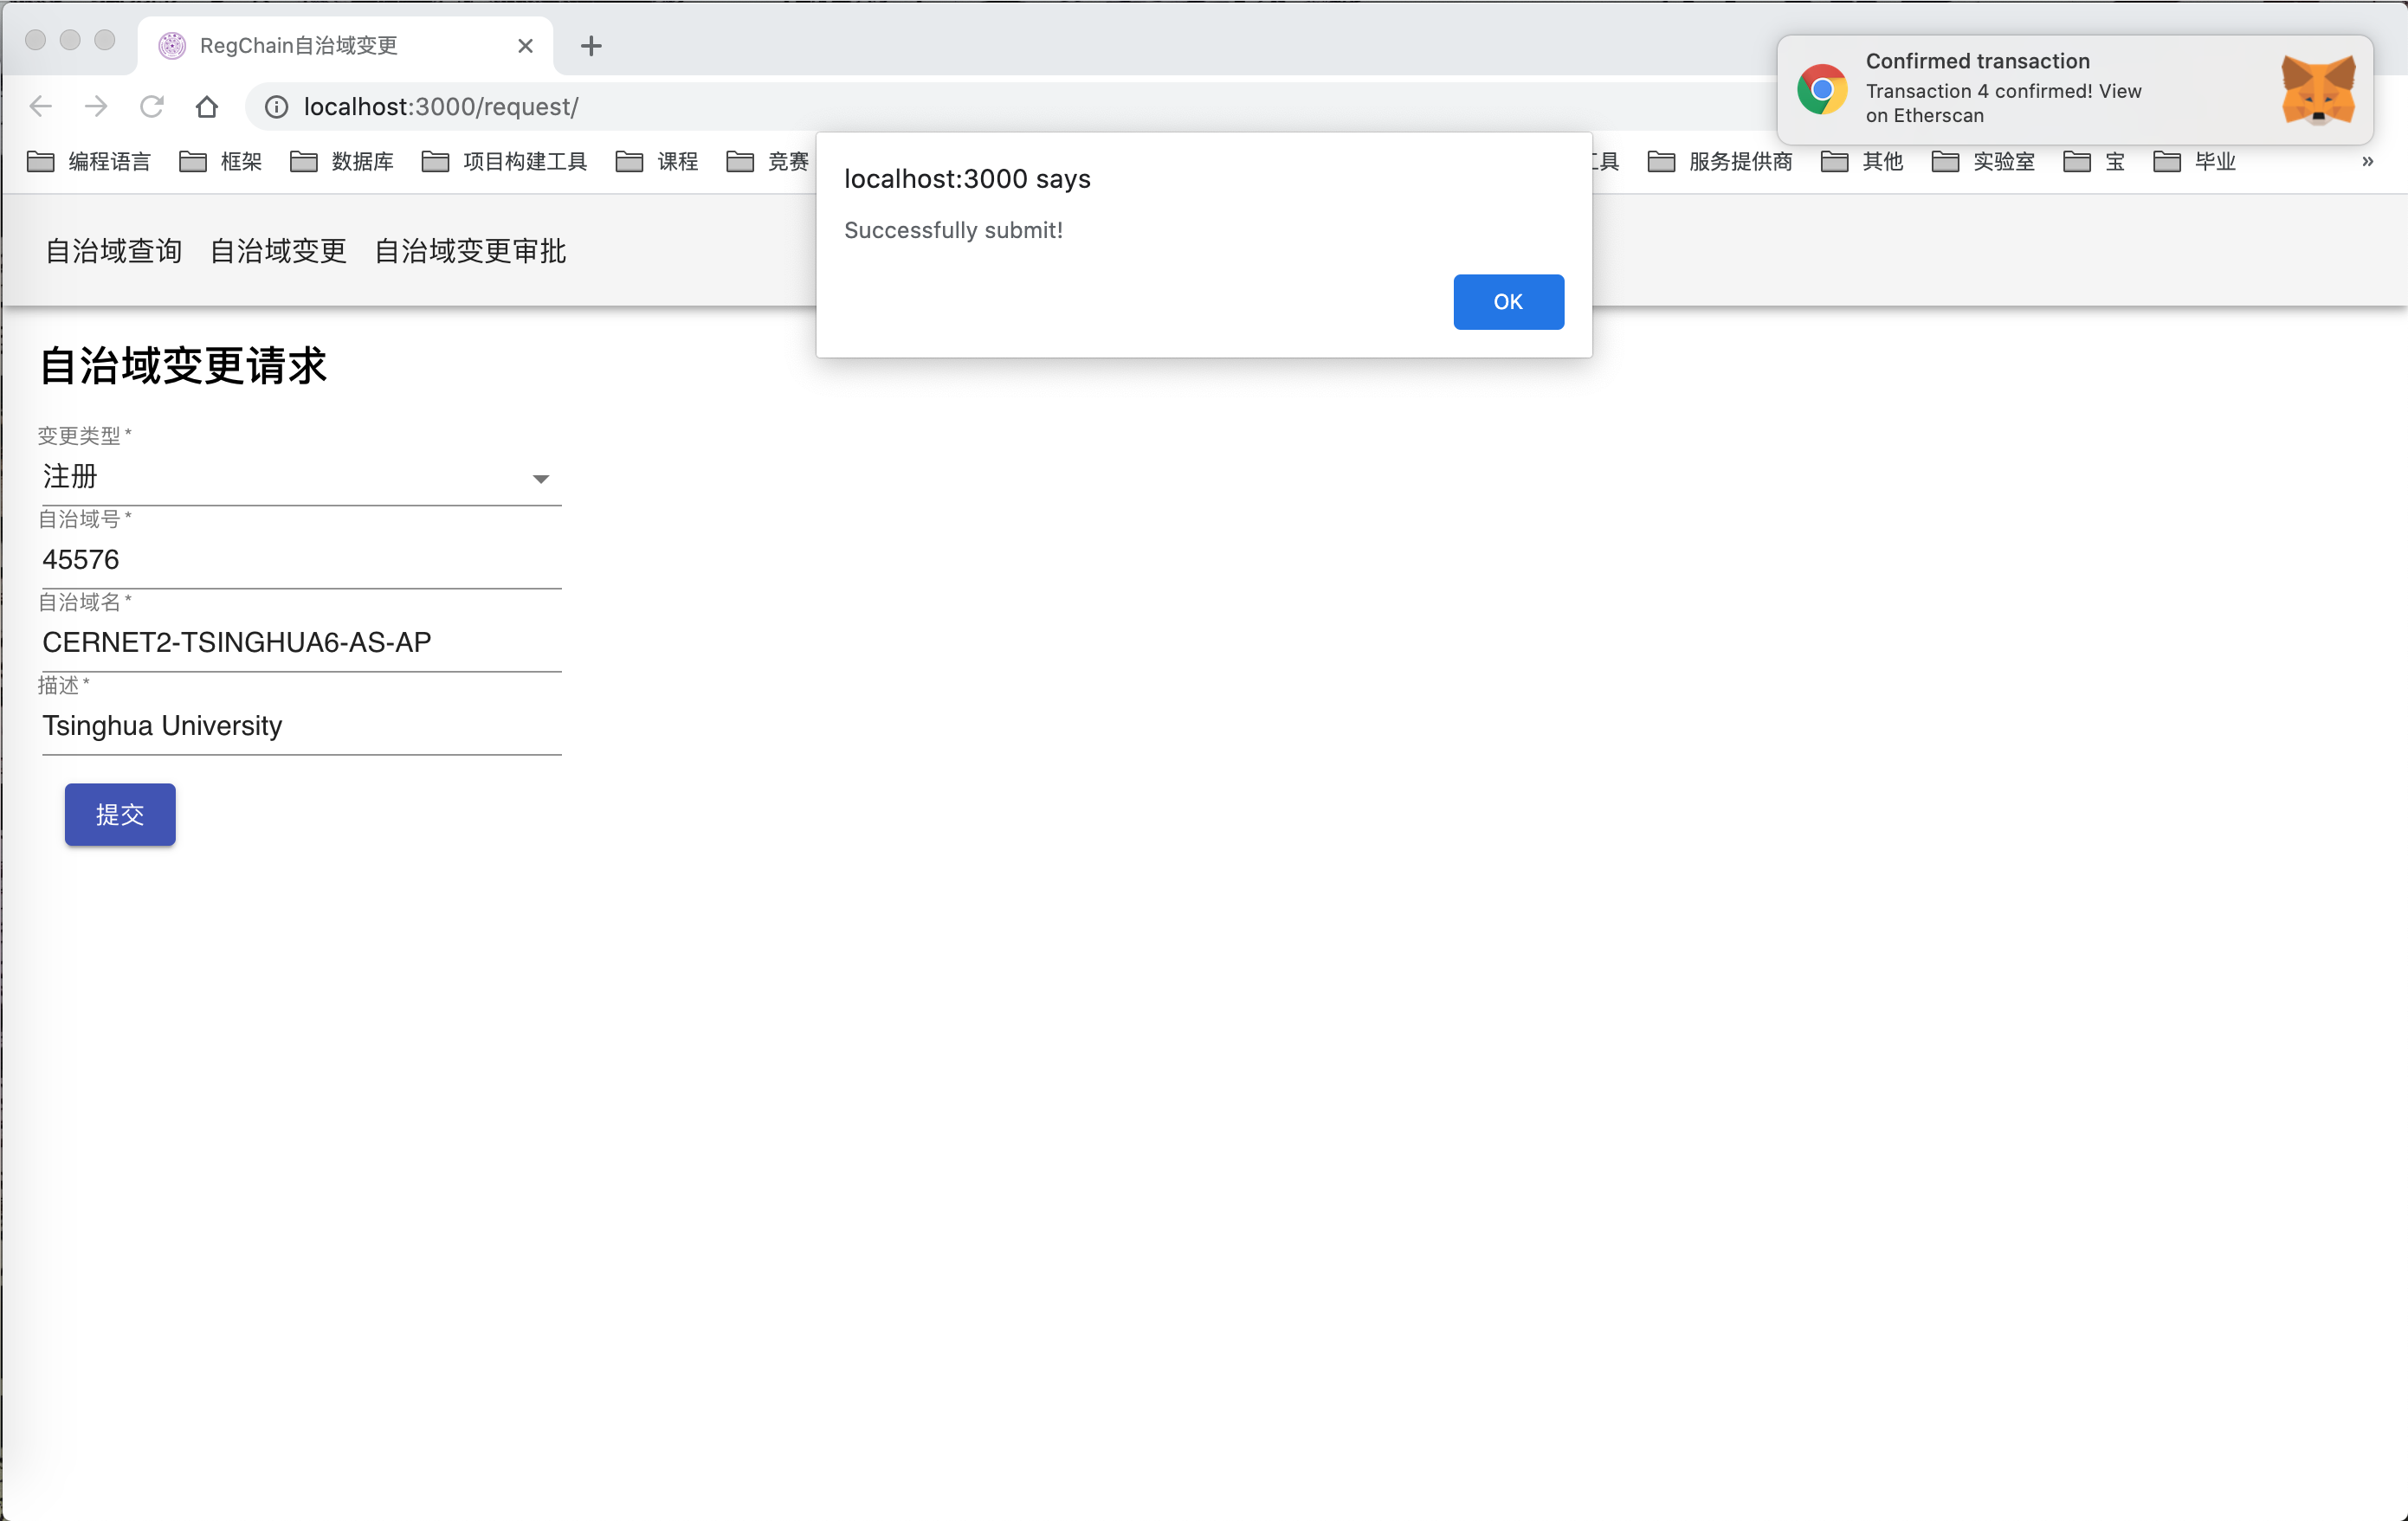
\includegraphics[height=4.5cm]{figures/regchain_client_request_2.png}}
        \caption{RegChain自治域申请页面}
        \label{fig:regchain_client_request}
      \end{figure}
      
      联盟管理员可通过“自治域变更审批”查看当前提交的自治域申请,并使用通过或拒绝按钮审批相应的申请,如图\ref{fig:regchain_client_review_1}所示。当非联盟管理员使用其他钱包尝试进行审批时,将被SMARegister所阻止,如图\ref{fig:regchain_client_review_2}所示。

      \begin{figure}[H]
        \centering
        \subcaptionbox{管理员正常审批\label{fig:regchain_client_review_1}}
        {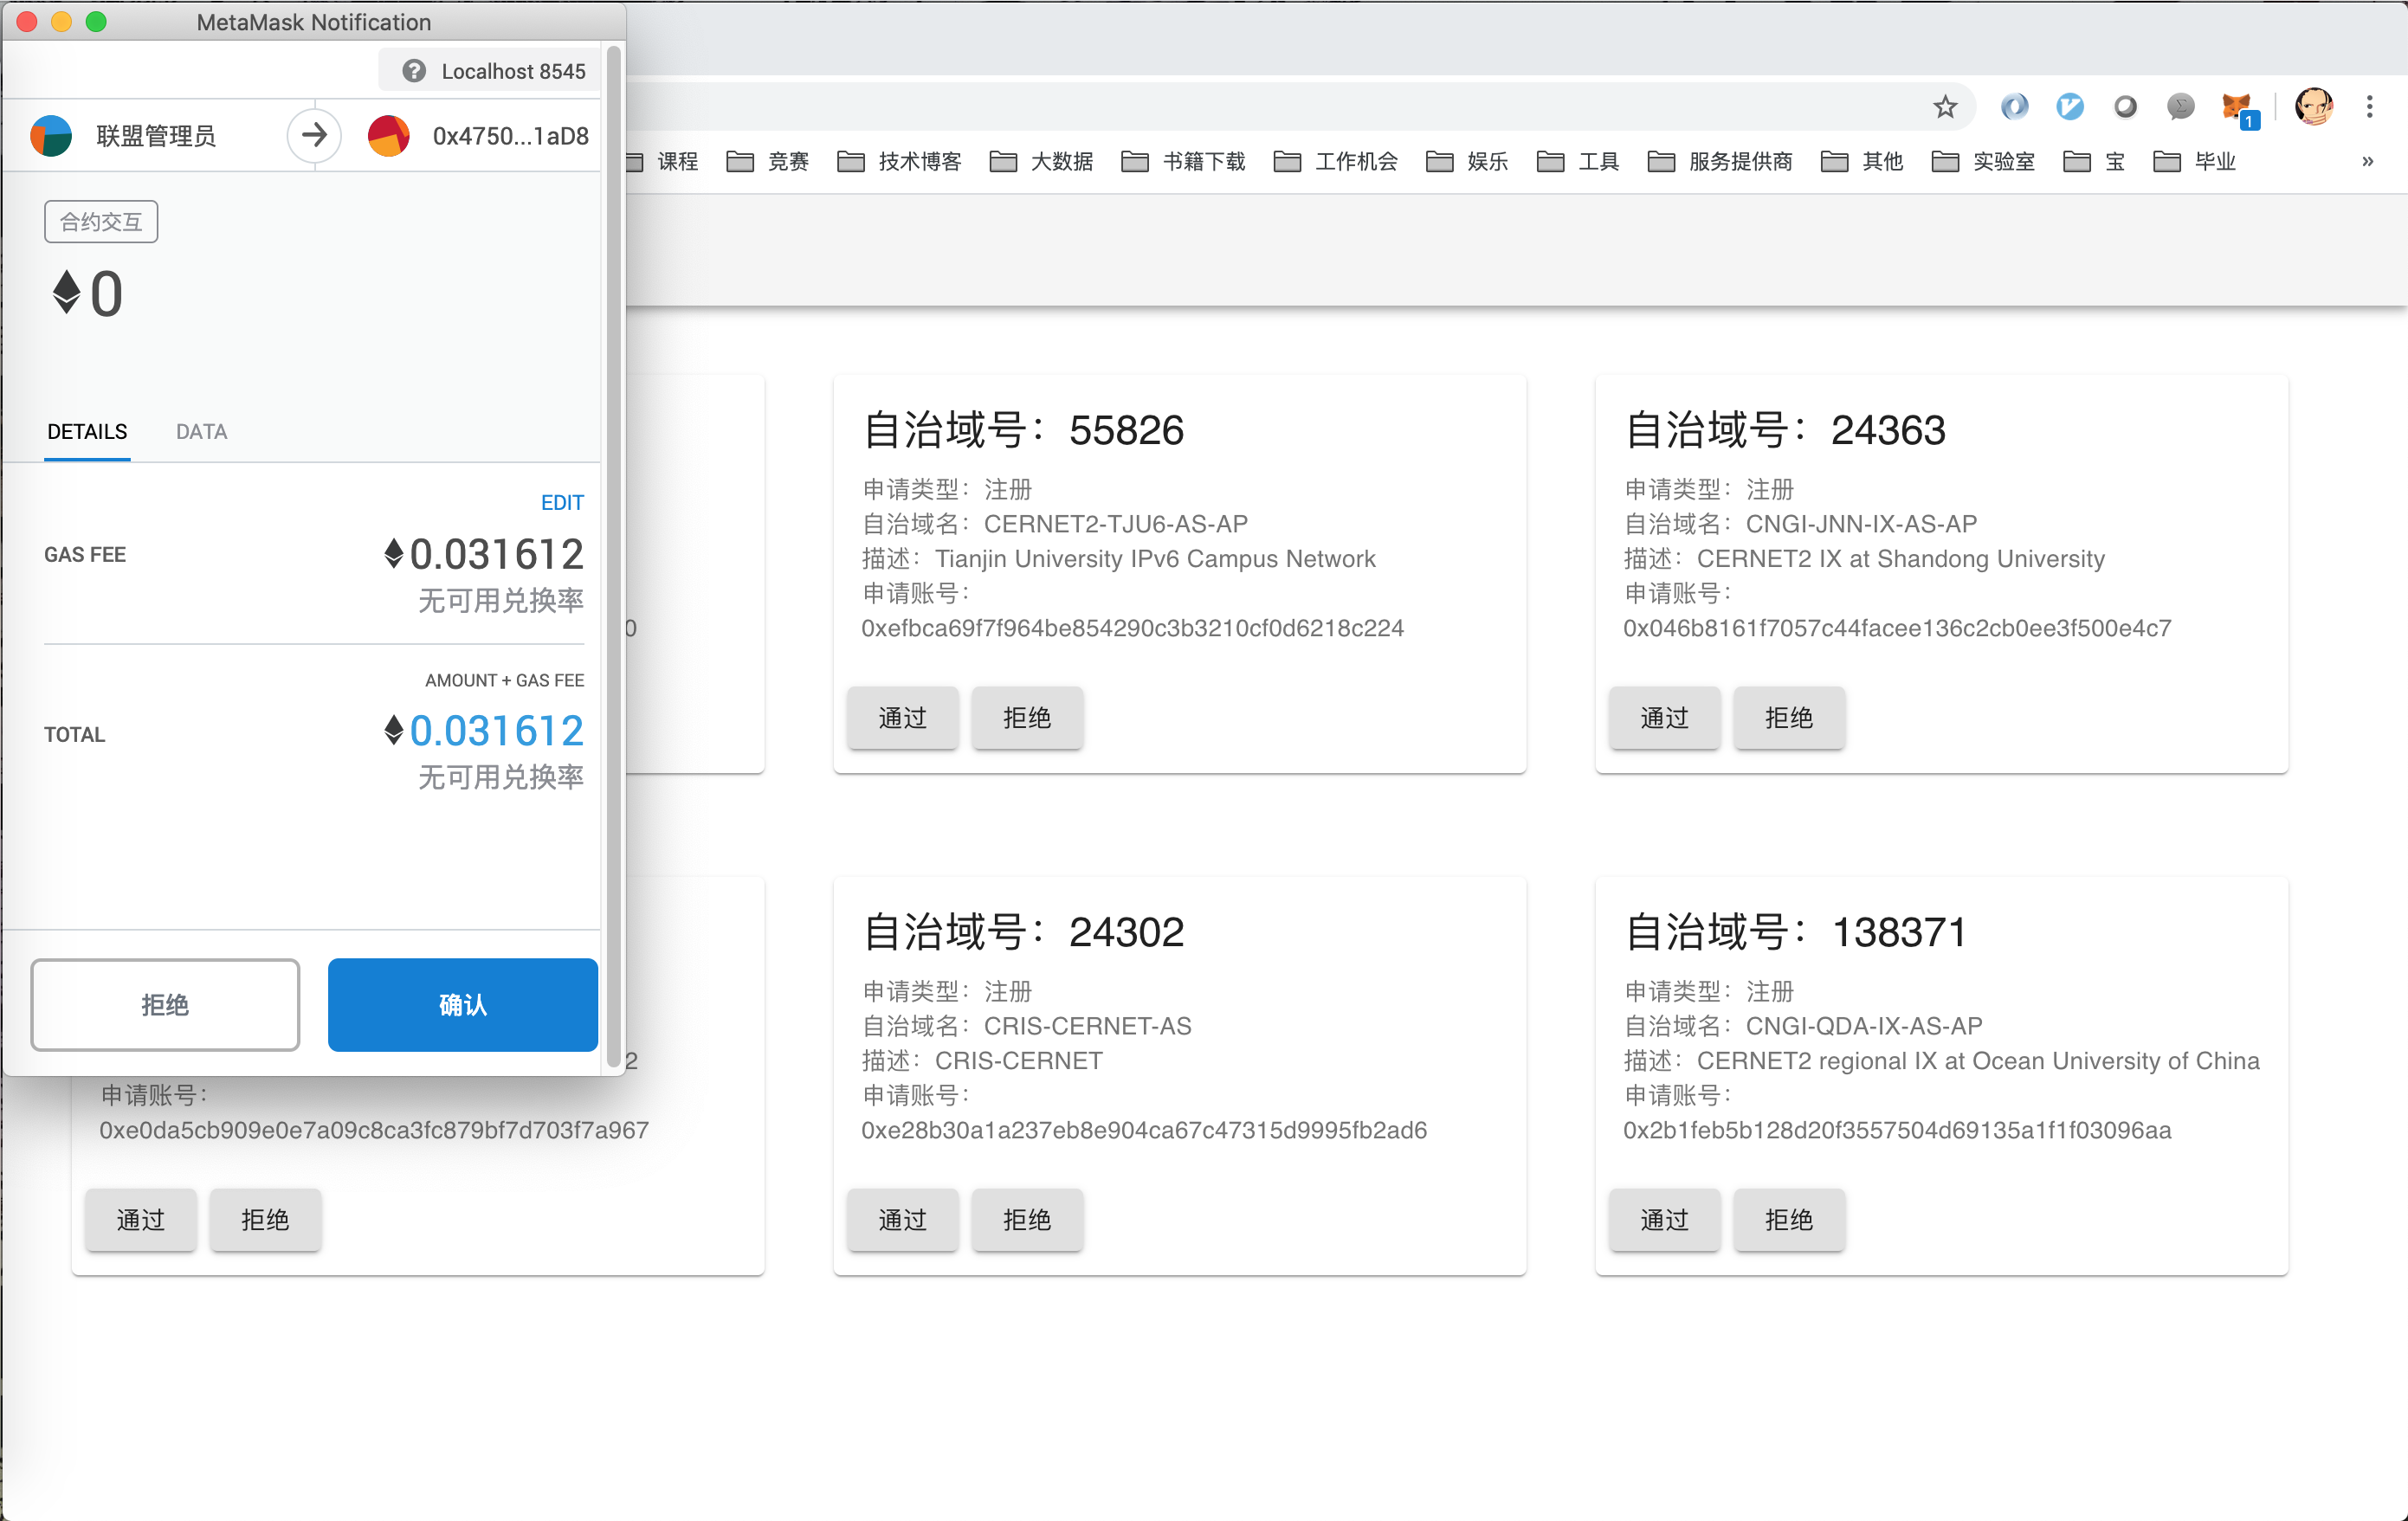
\includegraphics[height=4.5cm]{figures/regchain_client_review_1.png}}
        \hspace{1em}
        \subcaptionbox{非管理员无法审批\label{fig:regchain_client_review_2}}
        {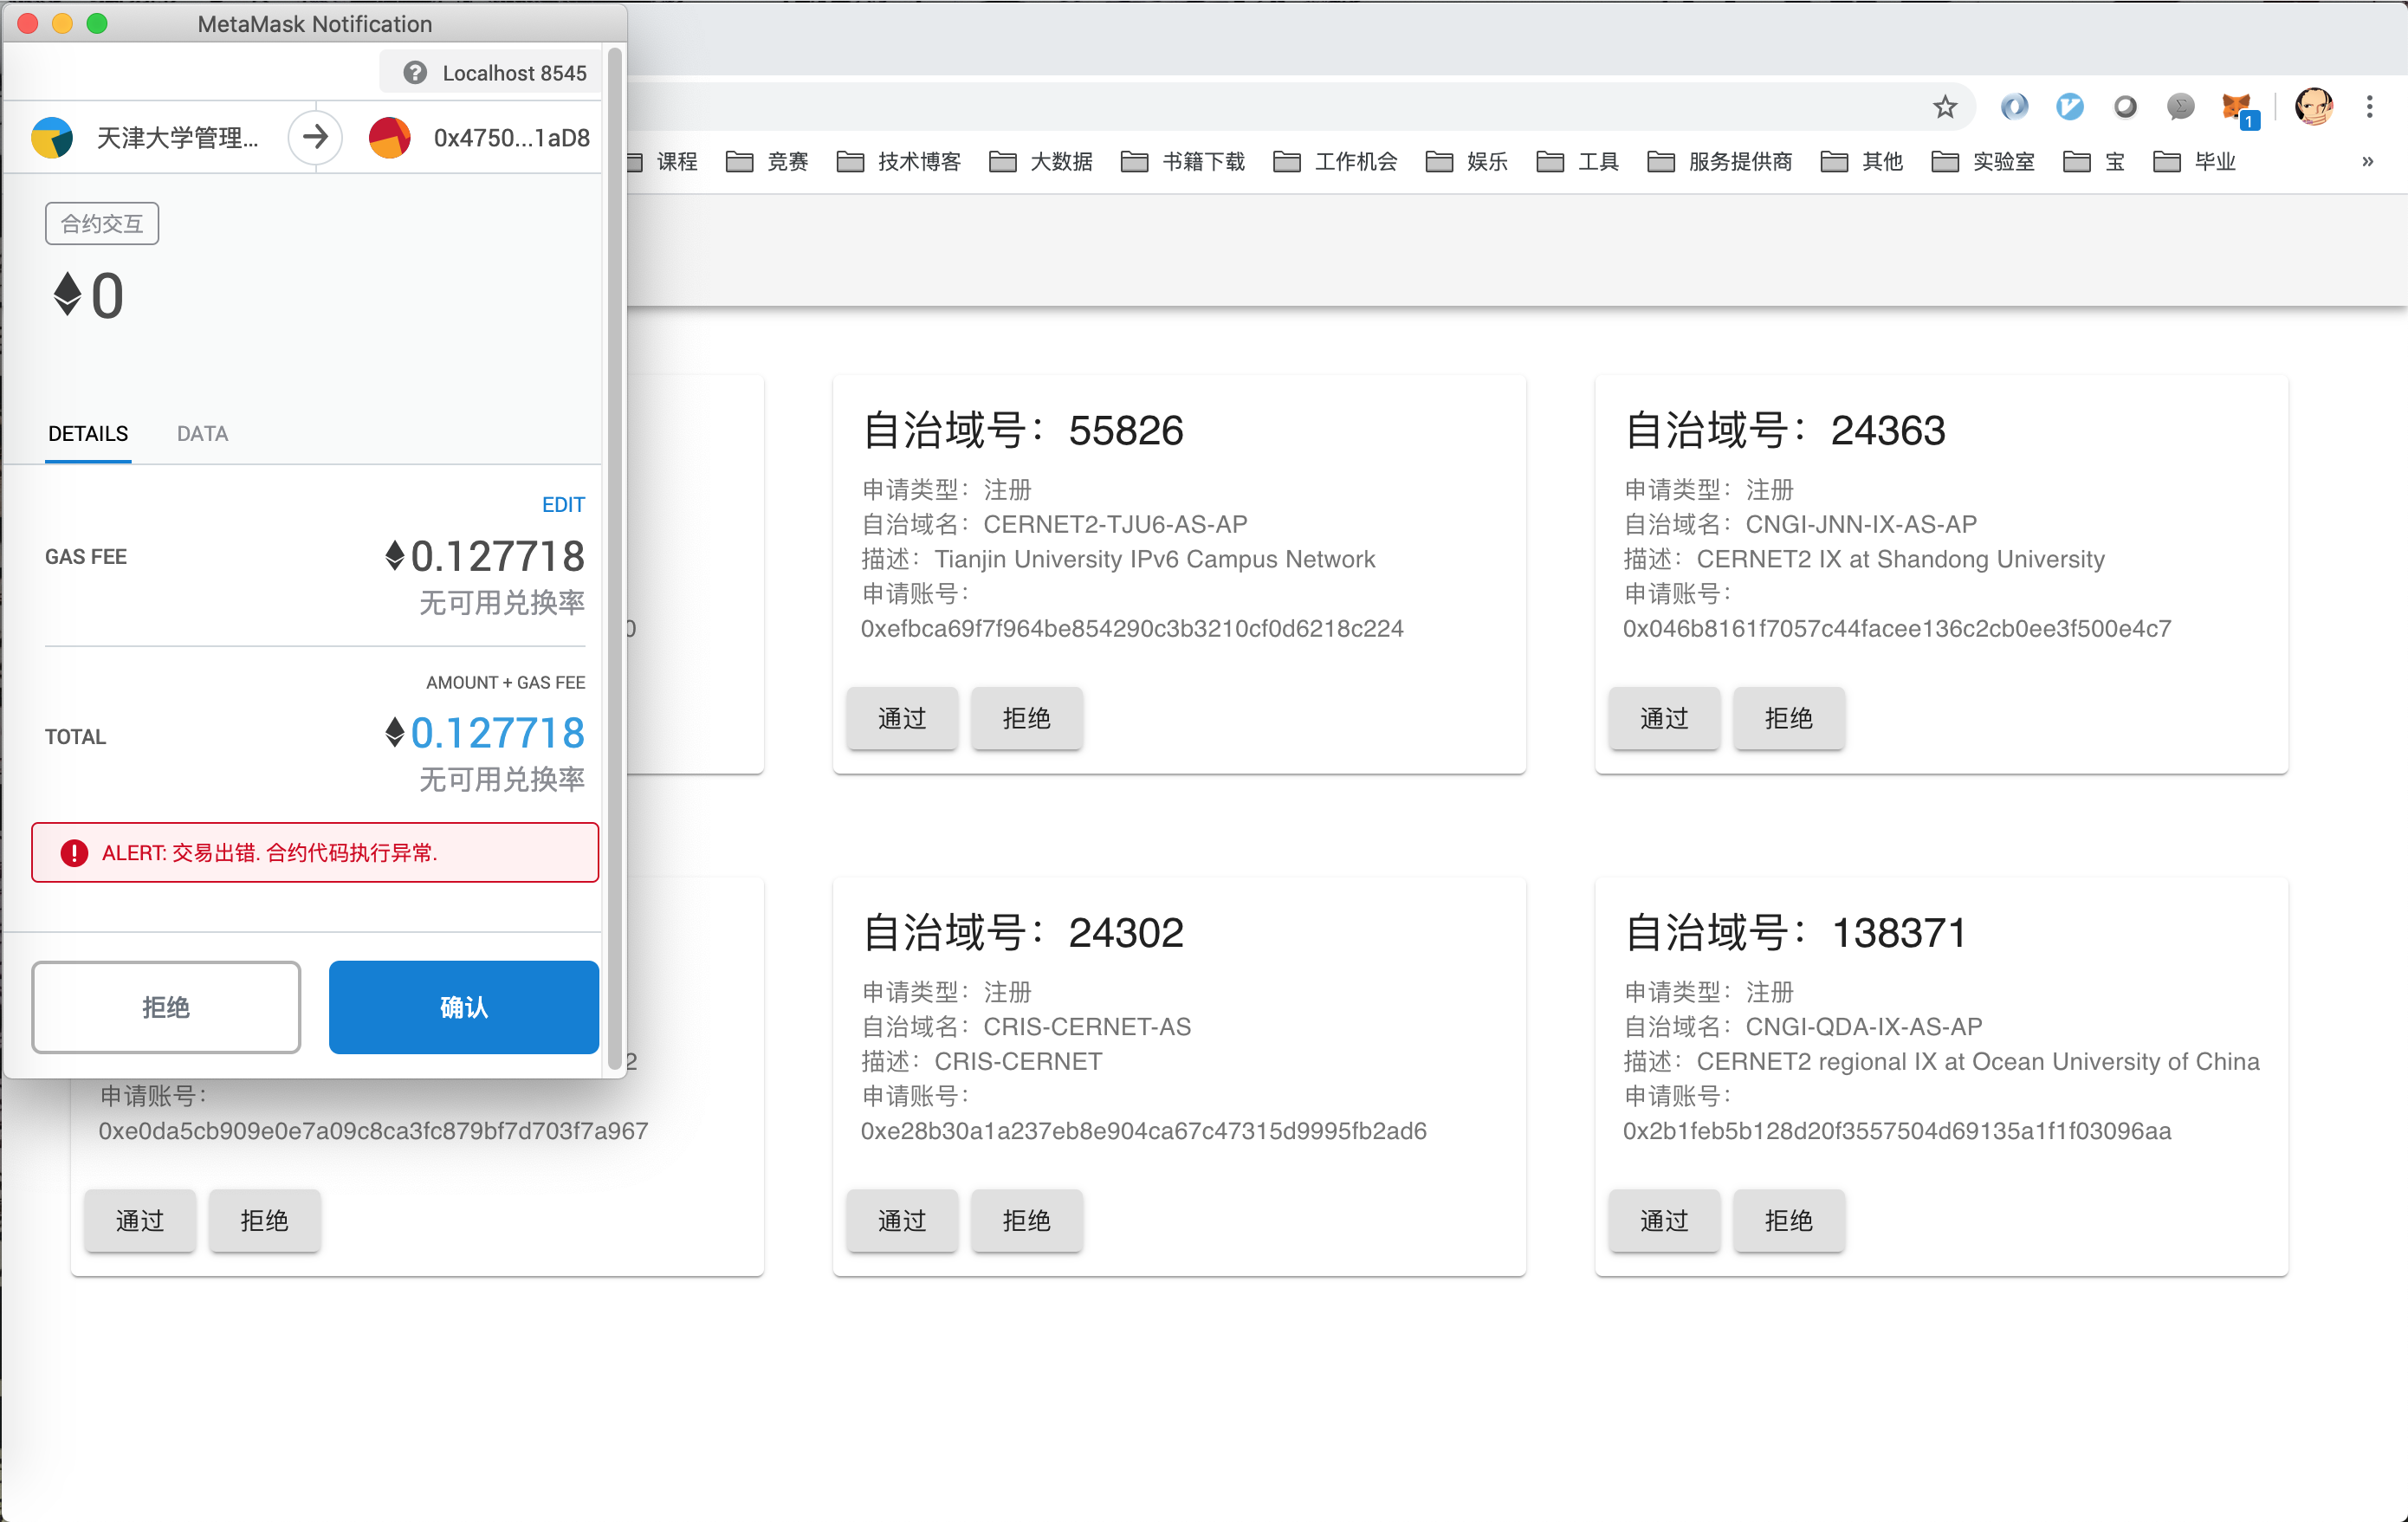
\includegraphics[height=4.5cm]{figures/regchain_client_review_2.png}}
        \caption{RegChain自治域审批页面}
        \label{fig:regchain_client_review}
      \end{figure}

      各个自治域管理员可通过“自治域查询”查看当前联盟内各个自治域的信息与当前有效的ACS地址。当点击自身管理的自治域显示卡时,将弹出窗口允许其对ACS信息进行配置,如图\ref{fig:regchain_client_update_1}所示。当点击其他自治域的显示卡时,也将弹出窗口显示具体信息,但不允许配置ACS信息,如图\ref{fig:regchain_client_update_2}所示,即使是联盟管理员也无法配置联盟内其他自治域的ACS地址。

      \begin{figure}[H]
        \centering
        \subcaptionbox{管理员正常更新\label{fig:regchain_client_update_1}}
        {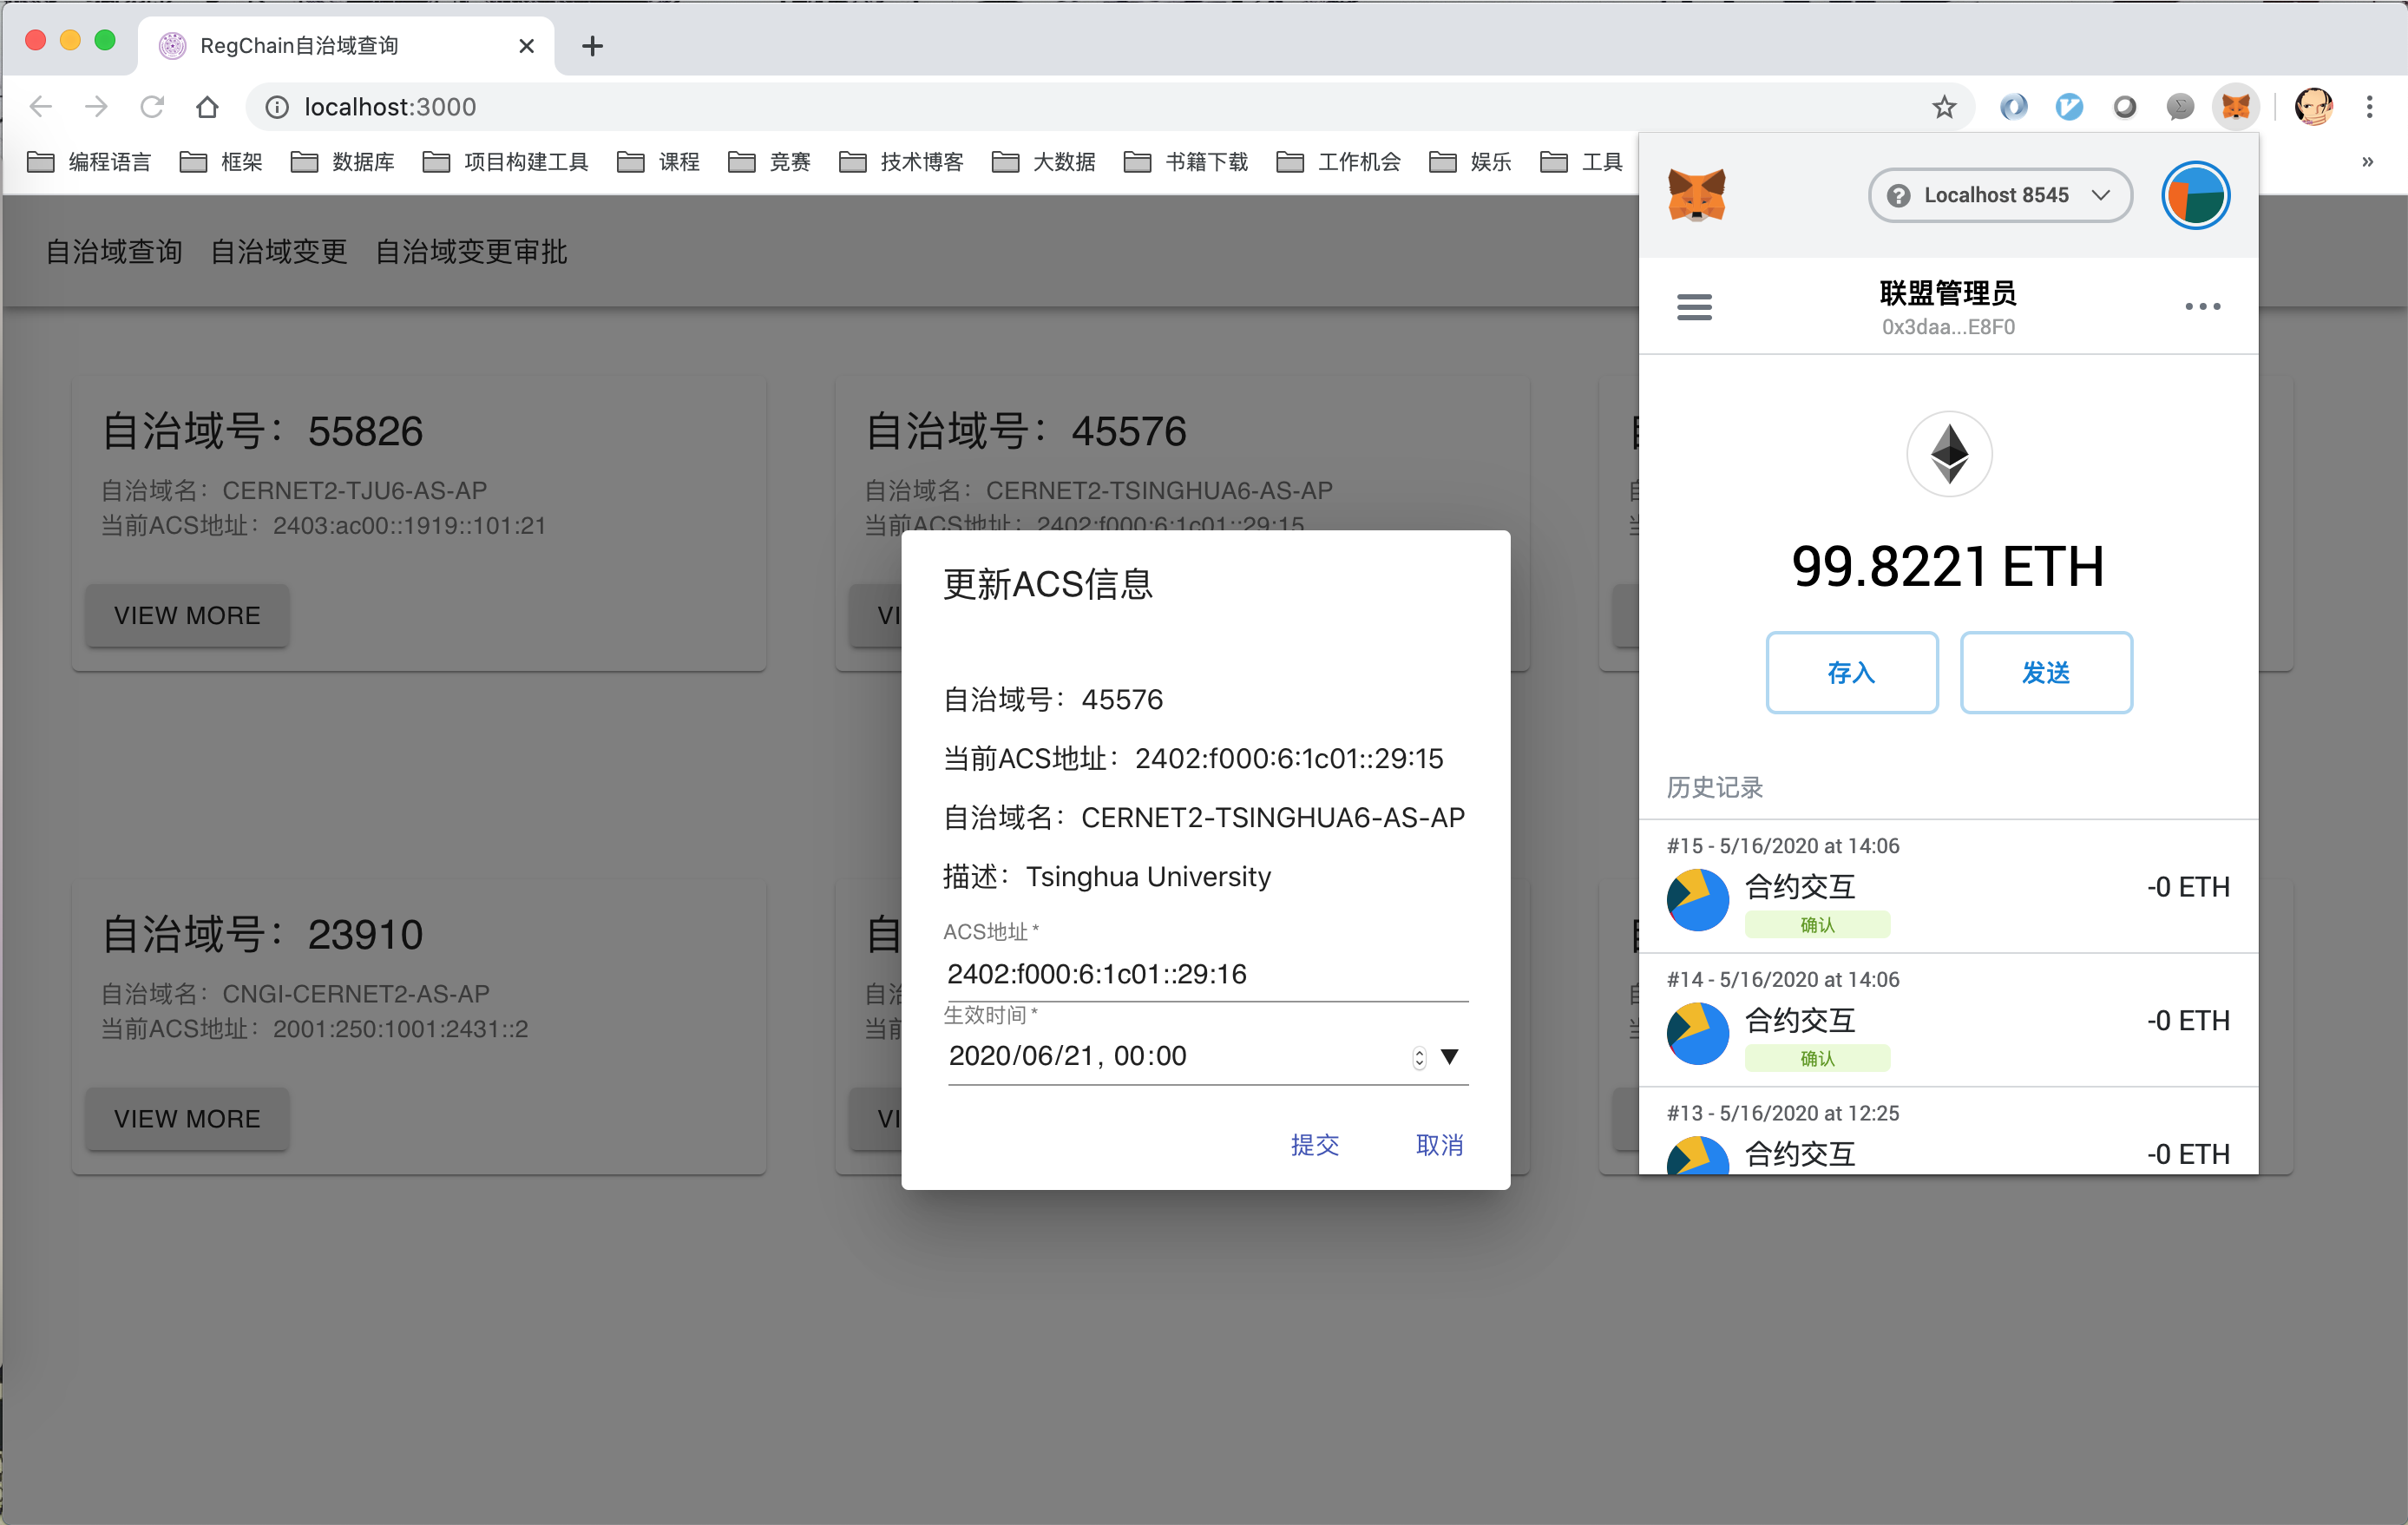
\includegraphics[height=4.5cm]{figures/regchain_client_update_1.png}}
        \hspace{1em}
        \subcaptionbox{非管理员无法更新\label{fig:regchain_client_update_2}}
        {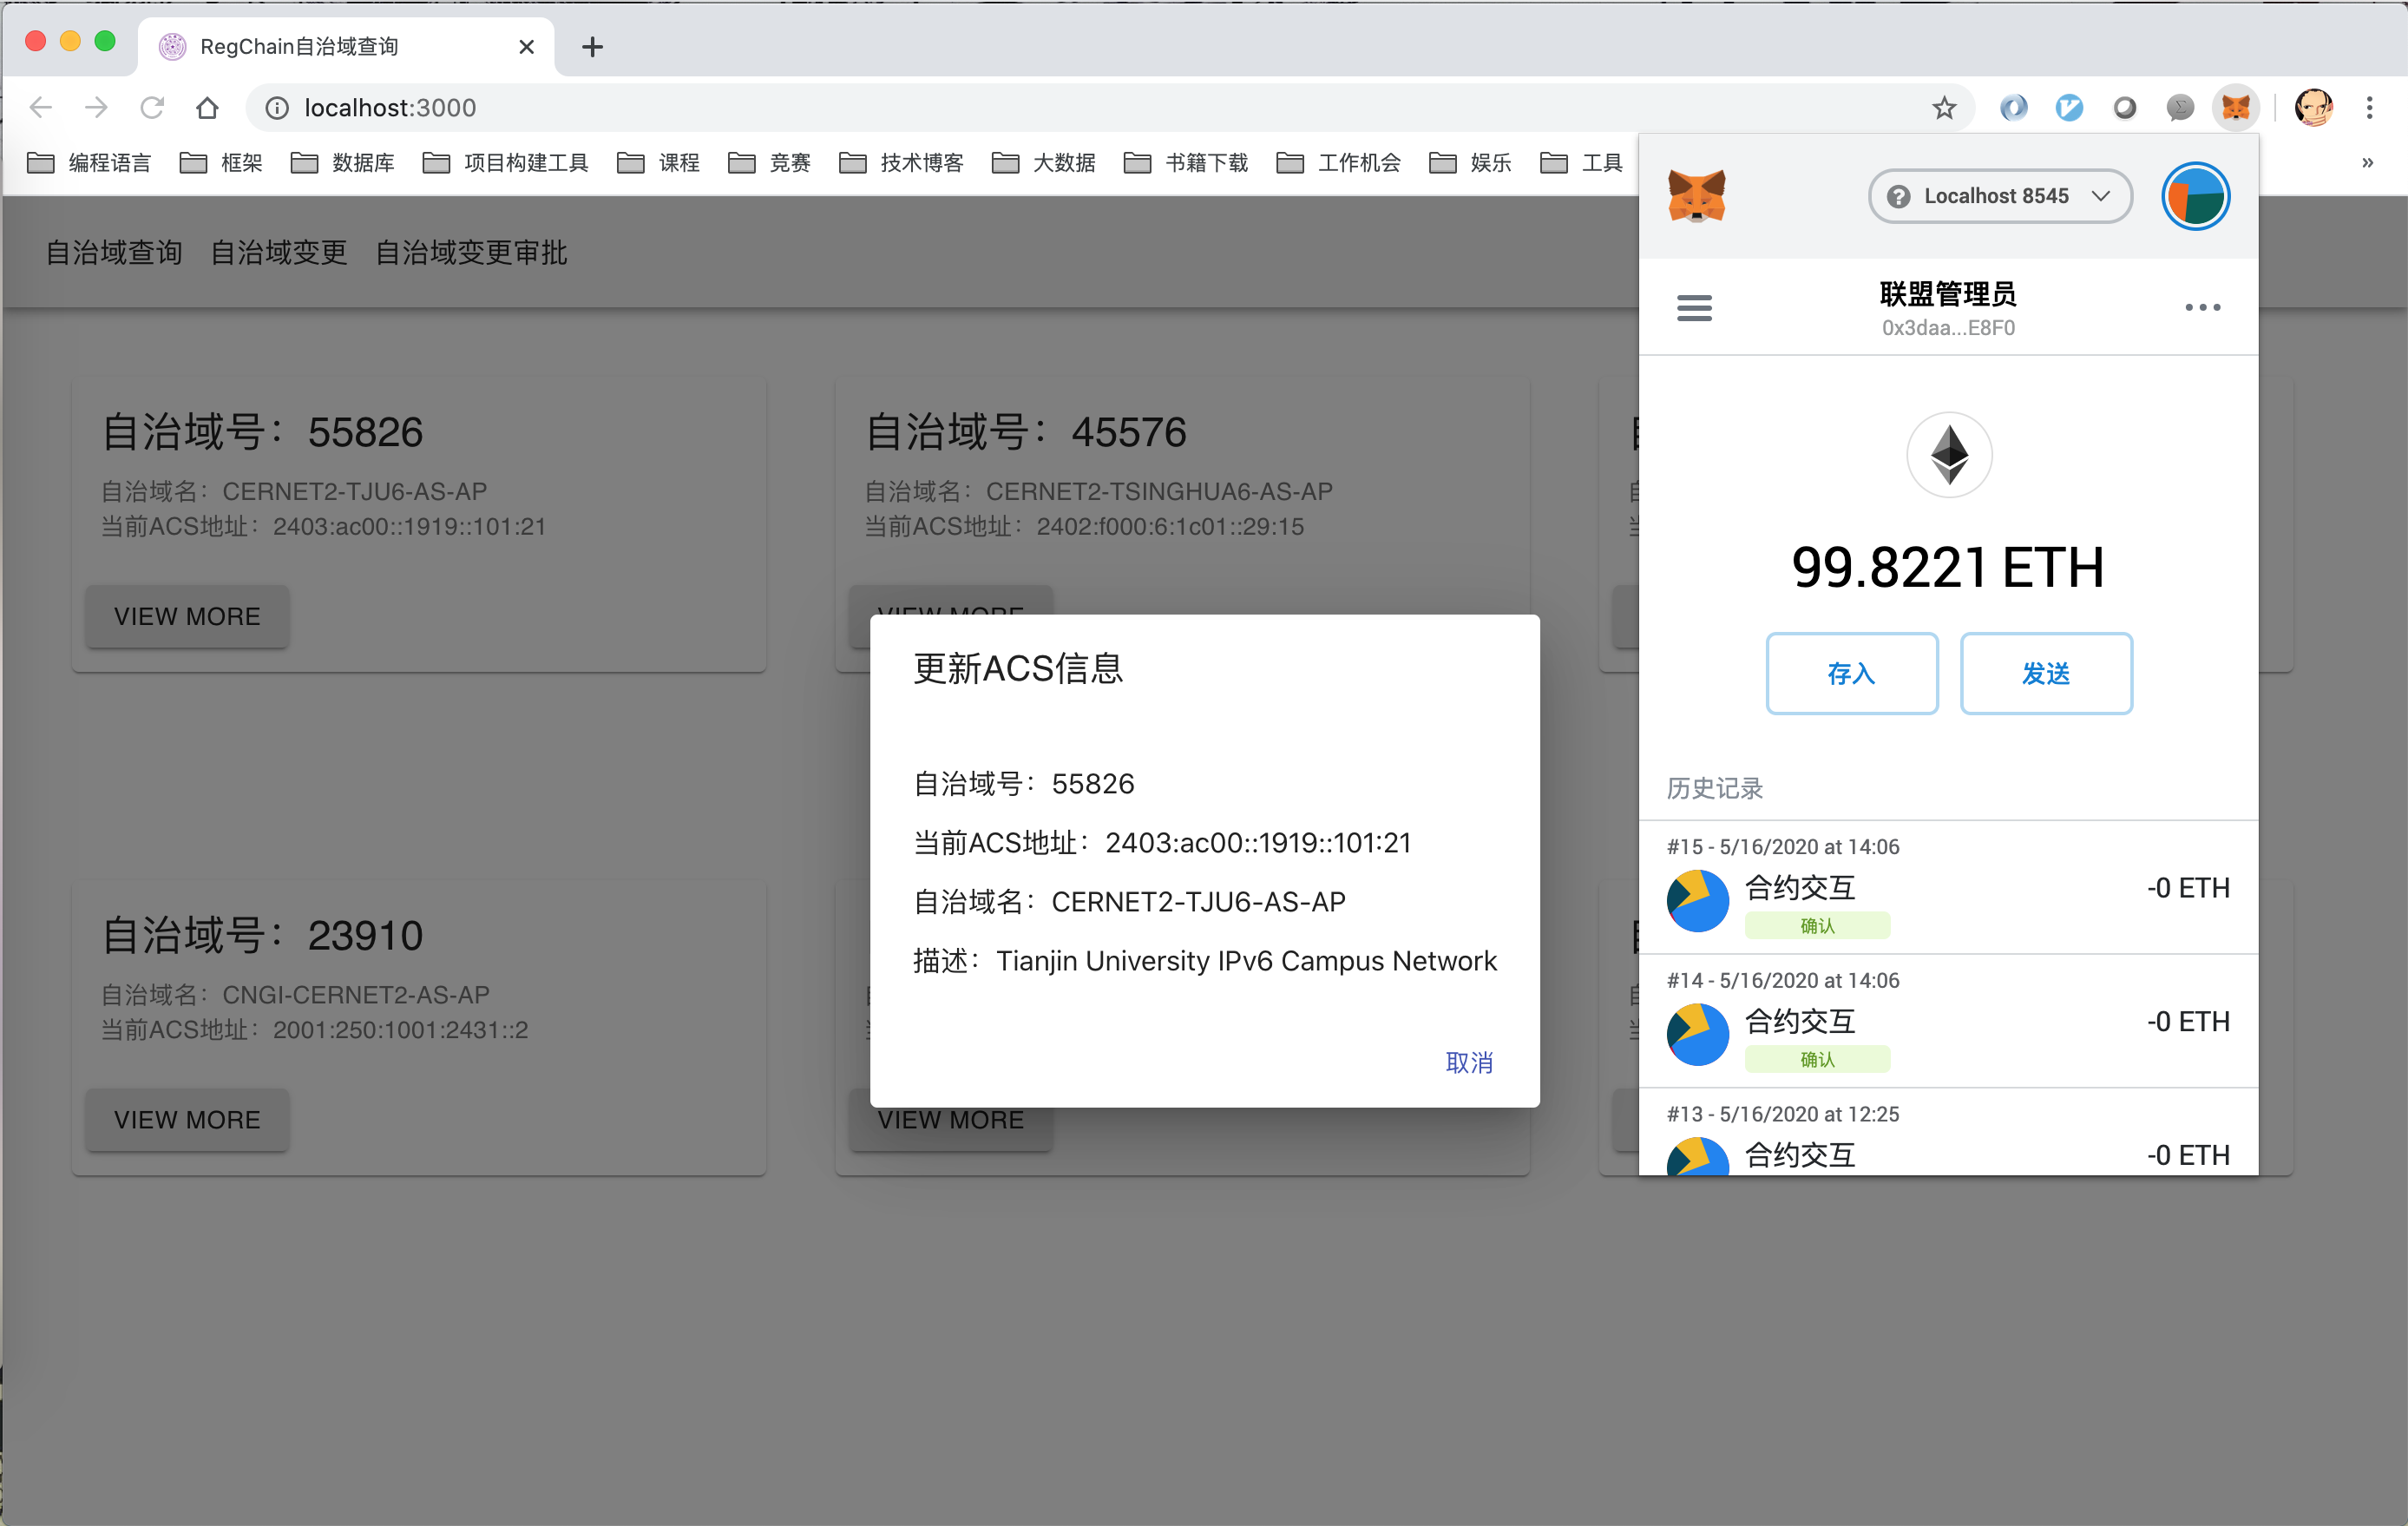
\includegraphics[height=4.5cm]{figures/regchain_client_update_2.png}}
        \caption{RegChain自治域ACS更新页面}
        \label{fig:regchain_client_update}
      \end{figure}

      自治域信息拉取服务的封装接口忽略了时间参数,其将自动根据系统时间计算当前时间进行参数填充,内部直接通过web3.js调用SMARegister.ASQuery与ASInfo.getCurrentACS获取联盟内所有自治域的当前ACS地址。

      \subsubsection{系统性能测试}
      \label{IPv6_Security:interas:implement:test}

      RegChain支持的各项操作由客户端与DApp两部分组成。自治域申请、审批操作在客户端仅需签发交易,在DApp侧则需要等待出块与合约执行。RegChain的出块速度与创建创世区块时设定的难度值相关,与RegChain的网络规模不相关,考虑到自治域信息更新操作要求的实时性不高,且并不频繁,本文在测试时将其难度值设定为0x4cccc8,以平均15秒的速度进行出块。

      本文以CNGI-CERNET2接入41所高校组成SMA安全联盟为例,采用41个区块链节点的网络规模对SMA联盟注册系统各项功能的性能进行了测试,结果如表\ref{tab:sma_ethereum_performance}所示。
      \begin{table}[htb]
        \centering
        \begin{minipage}[t]{\linewidth} 
          \caption{SMA联盟注册系统的以太坊实现性能测试}
          \label{tab:sma_ethereum_performance}
          \begin{tabularx}{\linewidth}{>{\centering\arraybackslash}X>{\centering\arraybackslash}X>{\centering\arraybackslash}X}
            \toprule[1.5pt]
            {\heiti 功能} & {\heiti 客户端时间(ms)} & {\heiti 合约时间(ms)} \\\midrule[1pt]
            {\heiti 自治域申请提交} & 8 & 69 \\
            {\heiti 自治域申请通过} & 7 & 69 \\ 
            {\heiti 自治域申请拒绝} & 7 & 50 \\ 
            {\heiti 自治域申请查询} & 6 & 131 \\ 
            {\heiti 单个ACS信息查询} & 7 & 13 \\ 
            {\heiti 全联盟ACS信息查询} & 7 & 71 \\ 
            \bottomrule[1.5pt]
          \end{tabularx}
        \end{minipage}
      \end{table}

      可见,由于各项操作在客户端处均为收集表单信息并发送交易,因此耗时基本相同。在DApp侧,自治域申请与审批操作由于需要向区块链中写入数据,因此耗时较多。自治域申请查询与ACS信息查询操作不需要更改区块链状态,但由于自治域数量较多,存在拷贝自治域信息的开销,因此尽管单个自治域查询时间极短,但进行全量查询时仍耗费了比自治域信息更新更多的时间。总而言之,各个操作均在远小于1秒的时间内完成,就用户体验而言拥有媲美单机服务器的性能。对于提交自治域更新或审批自治域更新请求等操作,至多等待15秒即可在区块链上看到相应数据的记录。

    \subsection{自治域间源地址验证技术安全性的进一步讨论}
    \label{IPv6_Security:interas:discuss}
    本文提出的RegChain方案主要针对自治域间源地址验证技术本身设计中的安全问题进行研究,其本质上是以一种避免数据篡改和降低服务不可用风险的分布式数据库替代了原本安全联盟采用的单点数据库,从而规避了因为联盟注册中心服务器的故障而导致整个联盟内跨自治域报文转发出现问题的风险,这种设计同样可以推广到其他所有基于安全联盟来建立自治域间信任关系的域间源地址验证方案中。对于其他的端到端类域间源地址验证方案,RegChain可根据其设计中安全联盟维护的信息对SMARegister与ASInfo的函数接口和内部数据结构进行相应的调整,从而适应不同格式的信息记录,为所有基于联盟的端到端类域间源地址验证技术提供统一的安全性提升方案。

    在SMA方案的设计中,各自治域持有的IPv6地址资源由自治域ACS之间建立通信协商状态机时进行公告,而非登记在RegChain中。尽管安全联盟机制能够保证一定程度的自治域间互信关系,但攻击者仍可能瞄准各自治域ACS发动攻击,篡改其宣告的IPv6地址以造成自治域间跨域报文转发的错误过滤等问题。RPKI\cite{RFC6480}可以提供对地址资源所有权的验证,从而解决宣告或使用虚假的IPv6地址的问题。但其同样面临单一故障点的困境,将其建设为区块链以分布式地记录地址资源所有权,可以进一步提升域间源地址验证技术的安全性,为用户身份识别与溯源系统提供更为牢固的IPv6地址真实性基础。

    本文所研究的RegChain方案属于论文作者所在实验室与华为网络技术实验室所合作的去中心化网络基础设施项目中的一部分,在该项目中还将研究利用区块链提升域间路由系统BGP\cite{RFC4271}、域名系统DNS\cite{RFC1034,RFC1035}等基础设施安全性的方案。

  \section{本章小结}
  \label{IPv6_Security:summary}
  本章从接入子网与自治域间两个层次的源地址验证技术分析出发,对SAVI技术在非理想网络环境中的部署问题与端到端类域间源地址验证技术的中心化风险分别提出了安全性增强的方案。主机粒度的源地址验证与跨自治域的源地址伪造预防是实现多组织用户身份识别与溯源技术的前提,这两者的增强方案的提出将进一步强化用户身份溯源机制带来的威慑能力。
% !TeX root = ../main.tex

\chapter{用户身份识别与溯源系统设计与实现}
\label{NIDTGA}

  \section{本章引言}
  \label{NIDTGA:introduction}
  NIDTGA地址生成方案\cite{liu2015building}作为一种致力于对用户身份进行溯源的IPv6地址生成技术,通过向IPv6地址接口标识中嵌入用户的网络身份标识NID与时间信息,能够减轻用户身份管理的复杂性,避免用户身份绑定信息的存储开销,并对管理域内用户的恶意上网行为产生有力的威慑作用。为了生成NIDTGA地址,需要首先获取用户身份,因此必须与网络中具体的认证手段相结合,而NIDTGA地址生成方案仅描绘了IPv6地址生成方案的蓝图,并未提出任何使用NIDTGA方案生成并配置地址的用户身份识别与溯源系统设计。事实上,由于实际的接入网络环境错综复杂,有线网络与无线网络组网方式有别,IPv6地址配置方式多种多样,用户接入认证手段迥异,而NIDTGA地址承载用户身份的能力将用户认证与地址配置相耦合,用户身份识别与溯源系统在各种网络环境下难以设计、实现与部署推广。NIDTGA地址生成方案理论与实践之间未加探讨的鸿沟严重阻碍了其应用与部署。本文针对这一问题,提出在实际网络中各种地址配置与用户认证方式下用户身份识别与溯源系统的设计方案,并进行了实现与部署测试,均以校园网为例探讨了各种组网方式下的网络设备配置要求,归纳了在中国下一代互联网示范工程(China Next Generation Internet-China Education and Research Network 2, CNGI-CERNET2)所连接的各大高校校园网络推广时的部署框架。

  为了便于讨论,本节首先定义用户身份识别与溯源系统中涉及到的几个实体概念如下:
  \begin{itemize}
    \item \textbf{用户}:用户是指从属于某一部署了用户身份识别与溯源系统的管理域并且采用NIDTGA地址接入上网的公民实体。
    \item \textbf{组织}:组织是指部署了用户身份识别与溯源系统的用户管理方,为用户提供使用NIDTGA地址的认证上网服务。
    \item \textbf{组织管理员}:组织管理员是指组织内负责运维用户身份识别与溯源系统的管理人员,负责用户身份识别与溯源系统相关设备的配置和运维、IDEA密钥的更新、用户上网行为管理等工作。
    \item \textbf{审计方}:审计方是拥有通过NIDTGA地址追溯用户身份权利的实体。由于溯源用户真实身份涉及到用户的隐私,因此这一权利必须谨慎控制,只能授权给具有相关权利的国家机构,比如国家安全中心等。溯源系统的运营与管理权限也由审计方进行控制。
  \end{itemize}

  本章内容组织如下:第\ref{NIDTGA:analyse}节分析用户身份识别与溯源系统在实际网络环境中进行设计与实现时的问题与难点,讨论了实现用户设备全覆盖需要适配的各种场景;第\ref{NIDTGA:DHCPv6}节研究DHCPv6地址配置方式下用户身份识别与溯源系统设计方案,比较了三种基于不同认证手段的设计方案的优缺点,并给出了各种设计方案的实现、部署与测试结果,并以最具推广性的基于二次认证手段的设计方案为例,总结了其在CNGI-CERNET2各校园网内的部署方案;第\ref{NIDTGA:SLAAC}节研究用户身份识别与溯源系统在SLAAC地址配置时的设计,指出基于SDN交换机的NAT方案的缺陷,设计了Web Portal与二层准入认证两种不同认证方式下的身份绑定技术;第\ref{NIDTGA:manual}节研究静态地址配置方式下的实现,讨论了校园网中静态地址配置策略向NIDTGA地址配置策略的迁移;第\ref{NIDTGA:summary}节对本章研究内容进行总结。

  \section{用户身份识别与溯源系统需支持的网络场景分析}
  \label{NIDTGA:analyse}

  在实际的网络环境中,用户通过认证接入网络获取地址的过程远比想象中复杂。首先,在网络侧,接入子网可以采用DHCPv6、SLAAC以及静态配置三种地址配置方式,认证手段则有Web Portal认证、IPoE与Web Portal结合的认证等三层认证手段,以及802.1X、PPPoE认证等二层认证方式,并且在无线网络与有线网络中数据报文转发方式又有着明显差异,各种技术排列组合形成了多样化的用户接入流程。在用户设备侧,不同的设备对地址配置方式、认证手段的支持又有所差异,比如搭载了Android、Chrome OS等Google系操作系统的设备由于操作系统内核中没有DHCPv6客户端模块,因此暂不支持DHCPv6配置IPv6地址,其他Windows、Linux等操作系统中虽然有着DHCPv6客户端,但是并没有完全支持DHCPv6标准中定义的全部功能,根据本文测试,目前还没有主流操作系统支持由DHCPv6服务器主动发起重新配置用户设备IPv6地址的Reconfigure报文。

  为了使NIDTGA地址生成方案能够得到部署和推广,用户身份识别与溯源系统必须能够对各类用户设备、各类接入子网地址配置与认证手段均加以支持,给出相应的设计与实现方案。不同的认证手段、地址配置方式均会对用户身份识别与溯源系统的设计流程产生影响,而接入网络的类型与数据报文转发模式则对用户身份识别与溯源系统的部署方案有着差异化的要求。

  本文对CNGI-CERNET2所连接的41所主要高校的组网方式进行调研后,统计结果如图\ref{fig:CNGI_CERNET2_statistic}所示。

  \begin{figure}[ht]
    \centering
    \subcaptionbox{有线网络\label{fig:CNGI_CERNET2_wired}}
    {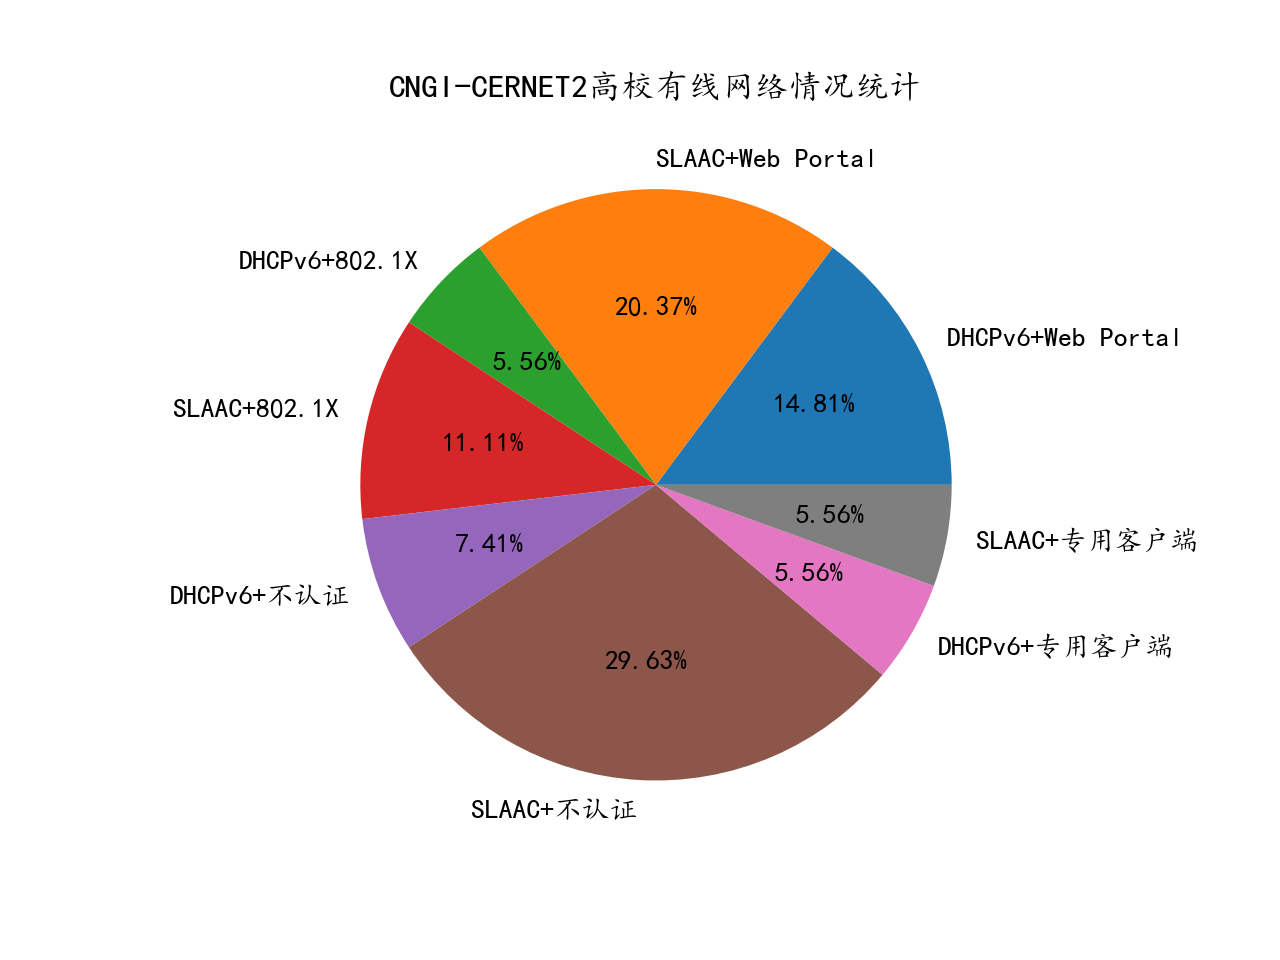
\includegraphics[width=0.49\textwidth]{figures/CNGI_CERNET2_wired.png}}
    \subcaptionbox{无线网络\label{fig:CNGI_CERNET2_wireless}}
    {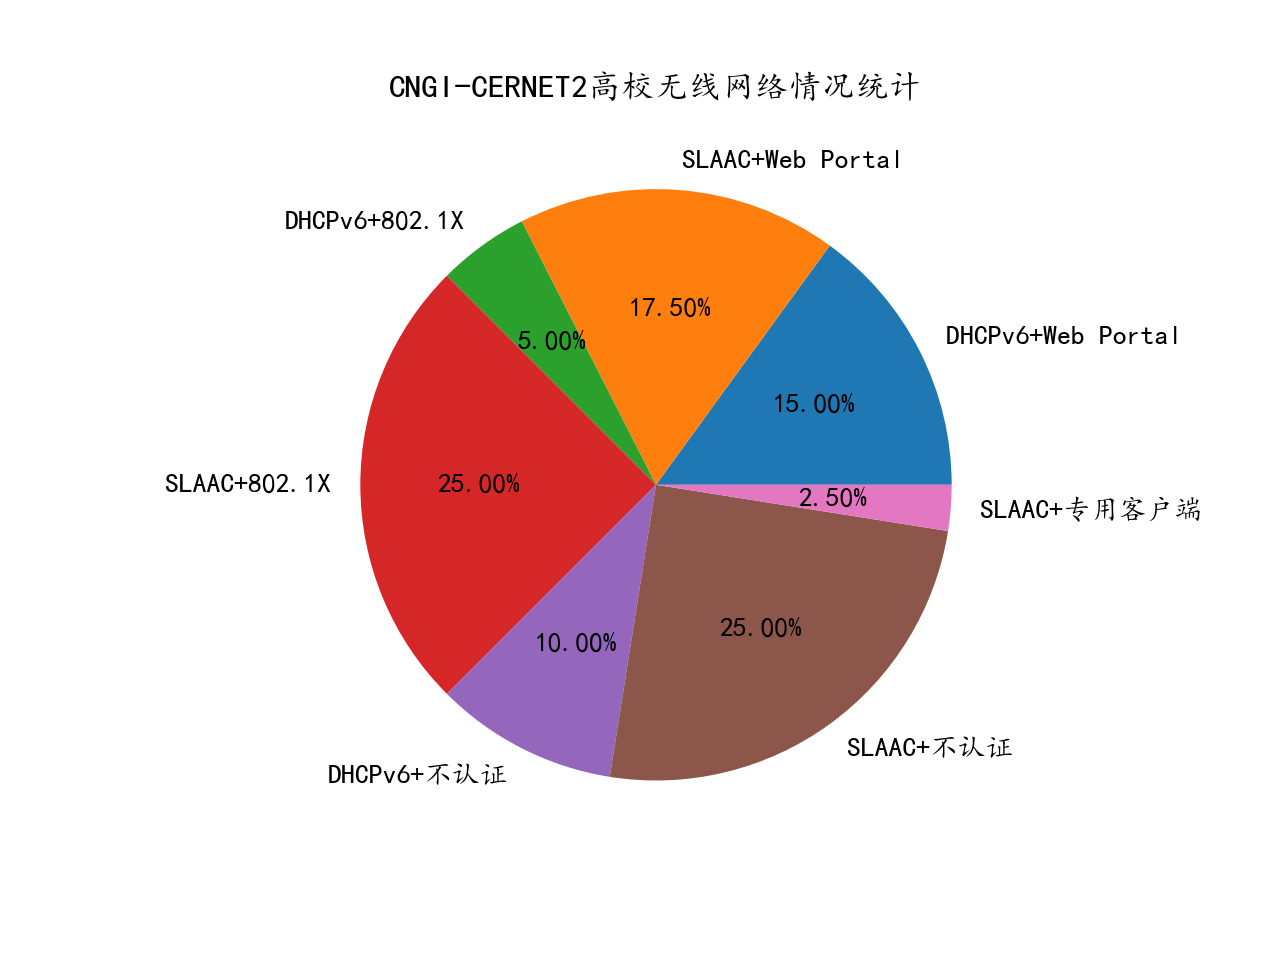
\includegraphics[width=0.49\textwidth]{figures/CNGI_CERNET2_wireless.png}}
    \caption{CNGI-CERNET2高校网络情况统计}
    \label{fig:CNGI_CERNET2_statistic}
  \end{figure}
  
  所有高校的无线网络全部采用基于无线控制器的架构,即各AP不能对自身进行配置和管理,仅仅作为WLAN系统中的一部分,而由AC对所有AP进行统一集中管理的组网模式。在基于无线控制器的无线网络架构下,尽管802.11以及用户认证相关的管理帧均由AP转发至AC处理,但用户发送的数据帧仍有集中转发与本地转发的两种模式。
  
  在用户认证手段方面,主要有802.1X认证、Web Portal认证以及不认证这三类方式,采用PPPoE以及其他定制客户端的认证手段较少。其中802.1X认证手段在无线网络中占比达30\%,远高于有线网络中的16.67\%,这是由于在无线网络中存在用户漫游的需求,802.1X认证方式能够在用户漫游时避免反复认证从而带来更友好的用户体验,而Web Portal认证方式由于其对设备连接性的支持较差,因此在无线网络中被采纳的比重有所下降。同时,对IPv6地址尚未进行用户认证管理的高校也占据了很高的比例,在有线网络与无线网络中分别为37.04\%与35\%。在各高校尚未对IPv6地址进行定制化管控时,向其推广部署用户身份识别与溯源系统面临的阻力将较小,更有利于向网络管理员建议采纳适宜用户身份识别与溯源的认证方式,因此本文将分析各类系统设计方案的优缺点,以选择最为合适的方案推动各高校部署。
  
  在地址配置方式上,DHCPv6与SLAAC两种方式在有线网络与无线网络中均有较大占比。在用户接入设备方面,无线设备主要是手机与笔记本,其中Android手机与iOS手机几乎占据了全部的手机份额,笔记本也以Windows系统与MacOS系统为主,通过有线接入的设备主要有个人电脑与静态配置地址的服务器,以及门禁、刷卡机等嵌入式设备。
  
  本文将各种常见的网络场景总结如图\ref{fig:NIDTGA_network_scenarios},其中忽略了对用户个人设备不进行认证这一类情况以推动各高校对IPv6地址实施管控,更好地支持用户身份识别与溯源系统的应用。可见,当面临实际应用落地时,用户身份识别与溯源系统需要支持大量的网络场景,每一种场景都要求用户身份识别与溯源系统进行定制的设计与实现。本文将以地址配置方式为一级分类,针对校园网络可能采取的认证手段设计与测试用户身份识别与溯源系统,并给出推广时的部署方案。

  \begin{figure}[ht]
    \centering
    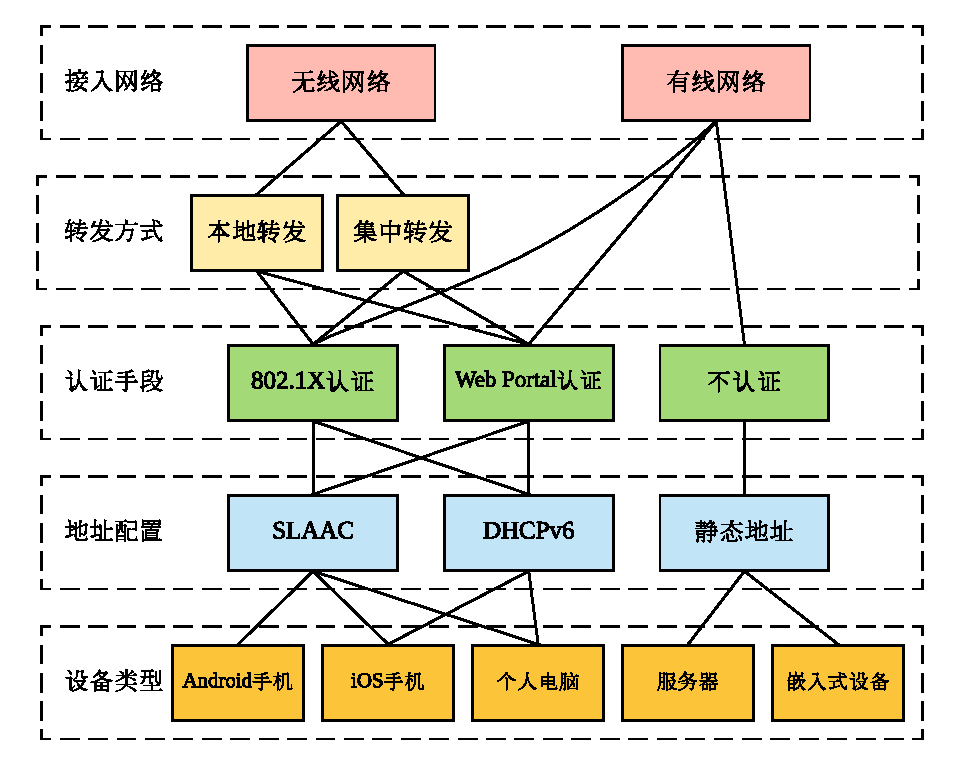
\includegraphics[width=0.9\textwidth]{NIDTGA_network_scenarios.pdf}
    \caption{用户身份识别与溯源系统需要支持的网络场景汇总}
    \label{fig:NIDTGA_network_scenarios}
  \end{figure}


  \section{DHCPv6下的用户身份识别与溯源系统}
  \label{NIDTGA:DHCPv6}
  由于DHCPv6采用集中式的有状态地址管理,用户接入时获得的IPv6地址由DHCPv6服务器决定,因此在DHCPv6配置地址的网络环境下适合采纳NIDTGA地址生成方案,并且一般不需要将其生成方案实现在用户设备端,有利于用户身份识别与溯源系统以用户无感知的方式推广部署。但是,由于NIDTGA生成地址时向IPv6接口标识中嵌入用户身份,因此用户接入网络时必须有身份认证这一过程,网络中不同的认证手段将影响到用户身份识别与溯源系统中认证系统与地址生成系统的交互逻辑。
  本节将首先给出用户身份识别与溯源系统在DHCPv6地址配置下的整体架构设计,然后对扩展DHCPv6认证、Web Portal认证与二层准入认证这三类认证方式下的设计方案分别展开探讨,并介绍各种方案的实现与部署应用情况,对三种方案进行对比和讨论,最后以校园网为例讨论基于二层准入认证的用户身份识别与溯源系统如何在无线网络与有线网络中进行部署推广。

    \subsection{用户身份识别与溯源系统整体架构}
    \label{NIDTGA:DHCPv6:architecture}
    本文设计的用户身份识别与溯源系统整体架构如图\ref{fig:DHCPv6_system_architecture}所示。系统中主要包含:
    \begin{enumerate}[1{)}]
      \item \textbf{认证控制设备}:网络中对用户接入进行认证控制的网络设备,一般为AC、接入交换机或宽带接入服务器等。用户所有流量均通过认证控制设备后才能进行跨子网的转发,认证控制设备将根据用户设备的认证情况,决定用户流量的转发策略。
      \item \textbf{认证管理服务器}:保存用户认证数据库信息的服务器。根据网络中认证手段的不同,具体形式将发生变化,在扩展DHCPv6认证时为一台记录了用户名与密码等匹配信息数据库的认证管理服务器;在采用Web Portal认证时,认证管理服务器将包含提供认证页面的Web Portal服务器与提供实际认证能力的AAA服务器;在二层准入认证时为AAA服务器。
      \item \textbf{密钥管理服务器}:向组织管理员提供NIDTGA地址生成密钥更新服务的网页服务器。组织管理员通过访问该密钥更新服务提交新密钥的更新请求,其负责将新密钥与生效时间发送给DHCPv6服务器与追溯服务器。
      \item \textbf{DHCPv6服务器}:采用NIDTGA地址生成方式为用户设备配置IPv6地址的服务器。在生成地址前需要与组织内的认证管理服务器同步可以用于标识用户的信息,比如用户设备MAC地址。
      \item \textbf{追溯服务器}:提供用户身份溯源服务的服务器。在单个组织内部署时,组织可自行部署一台追溯服务器以保存组织DHCPv6服务器上传的密钥更新历史。在用户身份识别与溯源系统在多个组织进行部署推广后,应部署一台全局唯一的追溯服务器,由具有用户身份溯源权限的审计方进行控制,用于保存各个组织的密钥更新历史,提供根据IPv6地址查询用户身份的服务。
    \end{enumerate}

    \begin{figure}[ht]
      \centering
      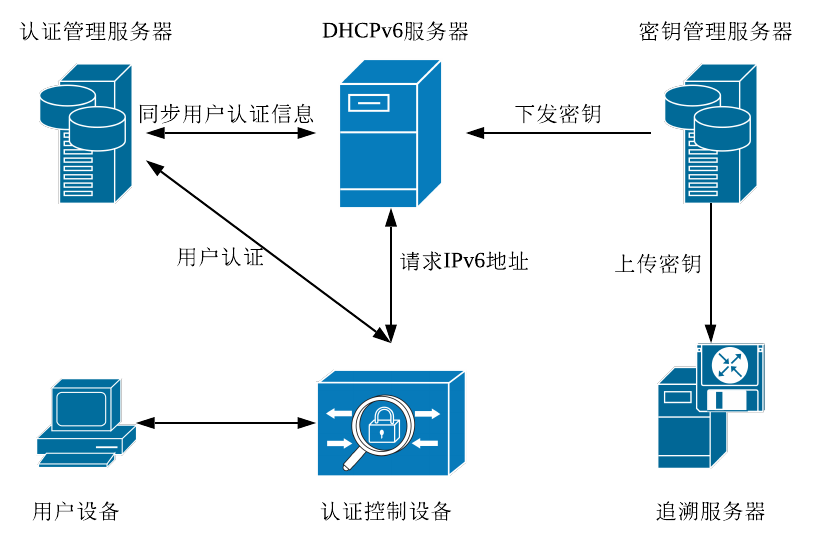
\includegraphics[width=0.7\textwidth]{DHCPv6_system_architecture.png}
      \caption{DHCPv6下用户身份识别与溯源系统整体架构}
      \label{fig:DHCPv6_system_architecture}
    \end{figure}

    在用户通过用户身份识别与溯源系统接入网络时,其数据流量将被认证控制设备阻截,必须首先完成用户身份的认证。认证管理服务器在用户通过认证后将标识认证用户的相关信息同步给DHCPv6服务器。在用户设备请求配置地址时,DHCPv6服务器将根据MAC地址等与用户设备相关联的标识,将请求地址配置的设备与已经完成认证的设备进行匹配,以确认用户身份并为其生成和配置NIDTGA地址。

    根据具体认证手段的不同,用户认证流程与认证管理服务器的形式都将发生变化,在认证管理服务器与DHCPv6服务器之间用于标识同一用户设备的信息也将发生变动,DHCPv6服务器内部生成与配置IPv6地址的逻辑也需要进行相应的更改。下面,本文针对三种不同的认证手段展开讨论,研究在不同的认证流程下用户身份识别与溯源系统的设计方案。

    \subsection{基于扩展DHCPv6协议认证的系统设计}
    \label{NIDTGA:DHCPv6:client}
    在网络中没有采用其他认证手段的情况下,仅通过DHCPv6协议完成用户身份的认证,必须扩展DHCPv6报文的语义,将用户的认证信息添加到DHCPv6报文中。尽管DHCPv6协议标准中没有定义用于携带用户身份信息的选项,但DHCPv6报文的结构使我们可以很容易地向其中添加自定义选项以支持用户认证。本文自定义DHCPv6选项如表\ref{tab:custom_dhcpv6_options}所示。
    \begin{table}[htb]
      \centering
      \begin{minipage}[t]{\linewidth}
        \caption{DHCPv6自定义选项表}
        \label{tab:custom_dhcpv6_options}
        \begin{tabularx}{\linewidth}{cc>{\centering\arraybackslash}X}
          \toprule[1.5pt]
          {\heiti 名称} & {\heiti 编号} & {\heiti 描述} \\\midrule[1pt]
          用户身份标识NID & 101 & 用于在Solicit报文与Request报文中携带用户NID \\ 
          随机数nonce & 102 & 用于在Advertise报文中携带用于密码哈希的随机数 \\ 
          密码MD5哈希 & 103 & 用于在Request报文中携带用户密码结合随机数使用MD5摘要算法哈希后的值 \\ 
          \bottomrule[1.5pt]
        \end{tabularx}
      \end{minipage}
    \end{table}

    同时,为了指示用户NID错误、密码错误等情况,本文利用DHCPv6标准的OPTION\_STATUS\_CODE选项(Option 13),对其携带的状态码进行扩展,可在DHCPv6服务器回复设备的Advertise报文或Reply报文中使用。自定义状态码如表\ref{tab:custom_dhcpv6_status_code}所示。
    \begin{table}[htb]
      \centering
      \begin{minipage}[t]{\linewidth} 
        \caption{DHCPv6自定义状态码表}
        \label{tab:custom_dhcpv6_status_code}
        \begin{tabularx}{\linewidth}{cc>{\centering\arraybackslash}X}
          \toprule[1.5pt]
          {\heiti 名称} & {\heiti 值} & {\heiti 描述} \\\midrule[1pt]
          NID错误 & 129 & 用于NID格式错误或NID在用户数据库中不存在等场景 \\ 
          密码错误 & 130 & 用于密码MD5值与用户数据库中密码的MD5值不匹配的场景 \\ 
          其他错误 & 131 & 用于DHCPv6服务器暂时无法分配IPv6地址的情况 \\
          \bottomrule[1.5pt]
        \end{tabularx}
      \end{minipage}
    \end{table}

    在未启用其他认证手段的DHCPv6配置地址网络中,当用户设备接入时,设备将收到网关公告的Managed位置位的RA报文,设备操作系统将使用内核协议栈中的DHCPv6客户端模块发起IPv6地址配置请求。但操作系统内核的协议栈是不支持自定义的DHCPv6选项的,因此用户身份识别与溯源系统必须在用户设备中禁用内核的DHCPv6客户端,采用定制的DHCPv6客户端输入用户NID与密码进行登录。

    DHCPv6服务器处需要维护用户地址预分配表与用户地址分配表,结构如表\ref{tab:custom_dhcpv6_preallocated}与表\ref{tab:custom_dhcpv6_allocated}所示。

    \begin{table}[htb]
      \centering
      \begin{minipage}[t]{\linewidth} 
        \caption{用户地址预分配表}
        \label{tab:custom_dhcpv6_preallocated}
        \begin{tabularx}{\linewidth}{>{\centering\arraybackslash}Xc>{\centering\arraybackslash}Xcc}
          \toprule[1.5pt]
          {\heiti 设备DUID} & {\heiti 用户NID} & {\heiti NIDTGA地址} & {\heiti 随机数nonce} & {\heiti 过期时间} \\\midrule[1pt]
          000100012537f6 19141877532dbe & 80002888b1 & 2402:f000:6:1c01: 6c28:70f1:be03:efe6 & 121 & 1583754484 \\ 
          \multicolumn{5}{c}{...} \\
          \bottomrule[1.5pt]
        \end{tabularx}
      \end{minipage}
    \end{table}

    \begin{table}[htb]
      \centering
      \begin{minipage}[t]{\linewidth} 
        \caption{用户地址分配表}
        \label{tab:custom_dhcpv6_allocated}
        \begin{tabularx}{\linewidth}{>{\centering\arraybackslash}Xc>{\centering\arraybackslash}Xc}
          \toprule[1.5pt]
          {\heiti 设备DUID} & {\heiti 用户NID} & {\heiti NIDTGA地址} & {\heiti 过期时间} \\\midrule[1pt]
          000100012537f6 19141877532dbe & 80002888b1 & 2402:f000:6:1c01: 6c28:70f1:be03:efe6 & 1583755084\\
          \multicolumn{4}{c}{...} \\
          \bottomrule[1.5pt]
        \end{tabularx}
      \end{minipage}
    \end{table}

    用户的认证流程如图\ref{fig:DHCPv6_custom_client}所示:
    \begin{enumerate}[1{)}]
      \item 用户在定制的DHCPv6客户端中输入NID与密码,点击登录。
      \item 定制DHCPv6客户端构建Solicit报文,添加NID作为Option 101,向链路中进行广播。
      \item DHCPv6服务器收到Solicit报文后,提取NID,将NID与当前时间拼接后使用IDEA密钥对其进行加密,生成NIDTGA地址。
      \item DHCPv6服务器构建Advertise报文,其中提供NIDTGA地址的配置,同时生成一个随机数作为Option 102添加到Advertise报文中,回复该设备,同时将该设备DUID、NID、NIDTGA地址、随机数nonce等关系插入表\ref{tab:custom_dhcpv6_preallocated}。
      \item 定制DHCPv6客户端提取Advertise报文中Option 102携带的随机数nonce,与用户密码拼接后,使用MD5信息摘要算法对其进行哈希,将NID作为Option 101、密码哈希值作为Option 103添加到Request报文中进行回复。
      \item DHCPv6服务器提取Request报文中携带的DUID、NID、密码MD5哈希值,根据DUID与NID查询表\ref{tab:custom_dhcpv6_preallocated}比较判断一致性,并获取对应的nonce。
      \item DHCPv6服务器将NID与nonce发送给认证管理服务器,获取对应用户密码与nonce值哈希后的密文,与用户Request报文中Option 103携带的值进行比较。
      \item 若用户认证成功,则构造Reply报文提供NIDTGA地址的配置信息,分配表\ref{tab:custom_dhcpv6_preallocated}中的NIDTGA地址,将对应表项从表\ref{tab:custom_dhcpv6_preallocated}中删除,并插入表\ref{tab:custom_dhcpv6_allocated}中;若用户登录失败,则构造Reply报文,携带指示失败的错误码回复用户设备,并删除表\ref{tab:custom_dhcpv6_preallocated}中的对应表项。
      \item 客户端根据Reply报文中提供的IPv6地址与租约时间等信息,配置用户设备的网络适配器,接入网络。
    \end{enumerate}

    \begin{figure}[ht]
      \centering
      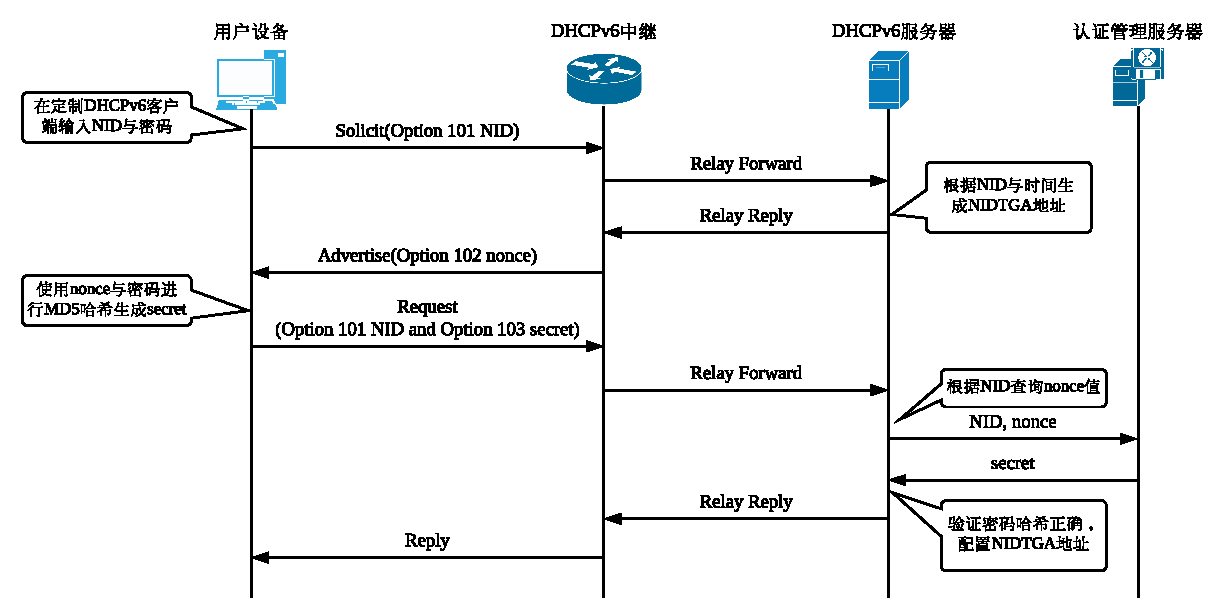
\includegraphics[width=\textwidth]{DHCPv6_custom_client.pdf}
      \caption{DHCPv6下扩展DHCPv6协议认证的用户身份识别与溯源系统时序}
      \label{fig:DHCPv6_custom_client}
    \end{figure}

    \subsection{基于Web Portal认证的系统设计}
    \label{NIDTGA:DHCPv6:portal}
    在大多数的网络环境中,为了限制网络资源的使用、对网络用户进行管理,网络管理者均会借助专用的认证手段对网络接入进行认证控制,其中Web Portal认证由于其轻量级和对用户的友好性得到了广泛的应用。在一般的Web Portal认证场景下,用户设备接入网络后,将根据标准的DHCPv6四步交互获得IPv6地址,认证控制设备将监听DHCPv6报文交互过程,与Web Portal认证系统进行交互,请求并记录包含设备所配置的IPv6地址、设备MAC地址等信息的绑定表项,表项中包含用户流量转发规则;当用户使用该IPv6地址访问网络时,若用户未认证、IPv6地址对应表项转发规则为重定向至认证系统,则认证控制设备将引导用户重定向至Web Portal认证网站;在用户认证通过后,Web Portal认证系统将下发该IPv6地址的新的流量转发规则给认证控制设备,允许该用户IPv6地址的流量访问网络。

    但是,NIDTGA地址生成逻辑与Web Portal认证的地址配置流程是冲突的:用户身份识别与溯源系统需要先获取用户身份后生成NIDTGA地址配置用户设备,而Web Portal认证则先配置设备IPv6地址后进行用户身份认证。没有获取IPv6地址则用户无法访问Web Portal进行认证,而不完成认证,用户身份识别与溯源系统又无法为用户设备生成NIDTGA地址并进行配置,用户认证与地址分配这两个过程在Web Portal认证手段下形成了一种死锁的关系。

    为了调和上述矛盾,我们需要采纳一种地址二次分配的过程:
    \begin{enumerate}[1{)}]
      \item 首先给用户设备分配一个用于访问Web Portal网站进行认证的临时IPv6地址,并指示认证控制设备对这类临时地址的流量始终进行重定向到Web Portal网站的操作;
      \item 在用户通过认证后,生成NIDTGA地址并对用户设备IPv6地址进行重新配置,并下发新的流量控制规则给认证控制设备。
    \end{enumerate}

    尽管DHCPv6标准\cite{RFC8415}中定义了由DHCPv6服务器对接入设备IPv6地址进行地址重配置的Reconfigure报文,但经过测试,目前通用设备的操作系统内核中的DHCPv6客户端均不支持对Reconfigure报文的处理,因此难以在DHCPv6服务器端主动发起地址重新配置的过程。在设备端,除去设备网络适配器重新连接网络的情况,重新配置地址的过程只在当前持有的IPv6地址续约时间来临时发起,因此必须将设备的临时IPv6地址租约时间设置得非常短,以确保用户在认证通过后迅速发起续约过程并重新配置地址。

    在这种情况下,DHCPv6服务器需要维护用户设备获取临时IPv6地址的状态与用户设备持有NIDTGA地址的状态,分别如表\ref{tab:web_portal_temporary}与表\ref{tab:web_portal_nidtga}所示。

    \begin{table}[htb]
      \centering
      \begin{minipage}[t]{\linewidth} 
        \caption{临时地址状态表}
        \label{tab:web_portal_temporary}
        \begin{tabularx}{\linewidth}{>{\centering\arraybackslash}Xccc}
          \toprule[1.5pt]
          {\heiti 设备DUID} & {\heiti 临时IPv6地址} & {\heiti 过期时间} & {\heiti 续约次数} \\\midrule[1pt]
          000100012537f619141877532dbe & 2402:f000:6:1c01::1 & 1583754484 & 3 \\ 
          \multicolumn{4}{c}{...} \\
          \bottomrule[1.5pt]
        \end{tabularx}
      \end{minipage}
    \end{table}

    \begin{table}[htb]
      \centering
      \begin{minipage}[t]{\linewidth} 
        \caption{NIDTGA地址状态表}
        \label{tab:web_portal_nidtga}
        \begin{tabularx}{\linewidth}{>{\centering\arraybackslash}Xc>{\centering\arraybackslash}Xc}
          \toprule[1.5pt]
          {\heiti 设备DUID} & {\heiti 用户NID} & {\heiti NIDTGA地址} & {\heiti 过期时间} \\\midrule[1pt]
          000100012537f6 19141877532dbe & 80002888b1 & 2402:f000:6:1c01: 6c28:70f1:be03:efe6 & 1583754484 \\ 
          00030001548998 923171 & 80002888b2 & 2402:f000:6:1c01: 12b7:1321:f025:1642 & 1583754943 \\ 
          \multicolumn{4}{c}{...} \\
          \bottomrule[1.5pt]
        \end{tabularx}
      \end{minipage}
    \end{table}


    本文设计Web Portal认证下的用户身份识别与溯源方案用户接入流程如图\ref{fig:DHCPv6_web_portal}所示:
    \begin{enumerate}[1{)}]
      \item 用户设备接入网络,通过标准的DHCPv6协议获取临时IPv6地址。
      \item DHCPv6服务器在收到用户设备的地址配置请求报文后,先根据设备DUID查询表\ref{tab:web_portal_nidtga},若不存在则从临时IPv6地址池中选择临时IPv6地址进行分配,租约时间设置为$T1=3s$,$T2=5s$,即3秒发送Renew报文,5秒发送Rebind报文,并将用户DUID、临时IPv6地址等关系插入表\ref{tab:web_portal_temporary};否则将根据表\ref{tab:web_portal_nidtga}中对应表项为其分配NIDTGA地址。
      \item 在用户设备请求临时IPv6地址过程中,认证控制设备将与Web Portal认证系统交互,获取用户临时IPv6地址绑定表项,规则为将用户流量重定向至Web Portal网站。
      \item 用户认证前,用户设备可能在临时IPv6地址租约到期之际多次向DHCPv6服务器发送Renew报文进行续约,以确保用户能够访问Web Portal网站,DHCPv6服务器将更新表\ref{tab:web_portal_temporary}中相应的过期时间与续约次数,并根据续约次数调整临时IPv6地址的租约时间。
      \item 用户使用临时IPv6地址通过浏览器访问网络时,将被重定向至Web Portal网站。
      \item 用户提交NID与密码完成认证,通过后,Web Portal认证系统将认证用户的NID、临时IPv6地址发送给DHCPv6服务器。
      \item DHCPv6服务器向表\ref{tab:web_portal_temporary}中查询临时IPv6地址对应认证用户设备的DUID,并根据用户NID与时间生成NIDTGA地址,将DUID、NID、NIDTGA地址等信息插入表\ref{tab:web_portal_nidtga}中。
      \item 用户设备再次发起对临时IPv6地址的续约流程,DHCPv6服务器根据DUID查询表\ref{tab:web_portal_nidtga},若表中存在该DUID,说明用户已认证,则对其续约请求回复立即过期的租约时长,使其发起新的地址配置请求;当设备为NIDTGA地址续约时,DHCPv6服务器检查地址是否与表\ref{tab:web_portal_nidtga}中匹配,若是则回复为其正常续约的Reply报文。
      \item 用户设备续约临时IPv6地址获得的新租约时长为0后,立即通过标准的DHCPv6协议发起新的地址配置请求,DHCPv6服务器根据其DUID查询表\ref{tab:web_portal_nidtga},确认后为其配置NIDTGA地址,并更新表\ref{tab:web_portal_nidtga}中过期时间。
      \item 当认证控制设备一段时间内未检测到用户设备的数据流量时,其向Web Portal认证管理服务器发送用户下线请求,包含用户NIDTGA地址,Web Portal认证管理服务器将对应用户下线,并将NIDTGA地址发送给DHCPv6服务器通知其将用户信息从表\ref{tab:web_portal_nidtga}中删除。
    \end{enumerate}
          
    \begin{figure}[ht]
      \centering
      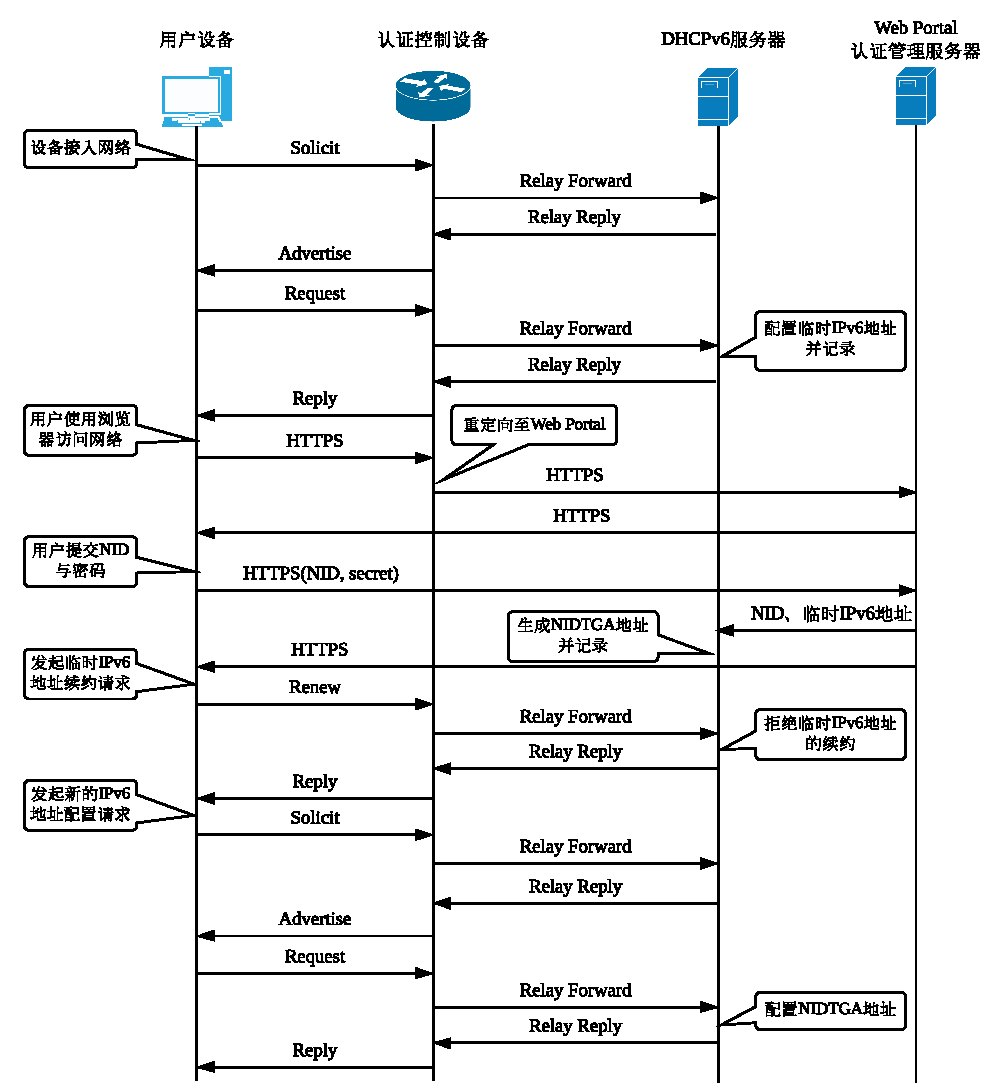
\includegraphics[width=\textwidth]{DHCPv6_web_portal.pdf}
      \caption{DHCPv6下Web Portal认证的用户身份识别与溯源系统时序}
      \label{fig:DHCPv6_web_portal}
    \end{figure}

    值得一提的是,由于临时地址的租约时间短,在未认证之前用户设备将频繁发起续约请求,对网络中的交换机等设备造成较大的负担,因此本文设计了对多次续约的临时地址租约时长进行调整的机制,以减轻网络设备的负担。DHCPv6服务器将在表\ref{tab:web_portal_temporary}中维护每个临时IPv6地址的续约次数,根据用户设备续约次数$n$,采取式\eqref{eq:T1_adjustment}对临时地址的T1时间进行调整,T2与过期时间将分别被设置为T1的$\frac{5}{3}$与$2$倍。
    \begin{equation}
      \label{eq:T1_adjustment}
      T1(n) = \left\{
      \begin{array}{rcl}
        3 & & {n \leq 40} \\
        6 & & {40 < n \leq 70} \\
        30 & & {n > 70}   
      \end{array}
      \right.
    \end{equation}

    本文在此对用户认证成功后配置NIDTGA地址所需的等待时间进行估算。当用户在获得临时地址后2分钟内完成认证,这是用户上网最为常见的情况,用户平均等待1.5秒,至多等待3秒即可获得NIDTGA地址访问网络;当用户在2分钟至5分钟内完成认证,则用户平均等待3秒,至多等待6秒;若用户在5分��内均未完成认证,则我们认为该用户暂时没有认证的意愿,其续约时长为30秒,故用户平均等待15秒,至多等待30秒访问网络。

    对于用户下线后又重新上线的情况,若NIDTGA地址已过期,则情况与用户新上线相同,否则其所需等待的时长与NIDTGA地址的租约时间有关。设DHCPv6服务器将NIDTGA地址的续约时间设置为$T$,用户下线距上一次续约的时长在0到$T$内均匀分布,概率密度为$\frac{1}{T}$。将用户下线后重新上线的行为建模为强度为$\lambda$的泊松过程。设$t$为用户设备IPv6地址最后一次续约至用户下线之间经过的时长,那么在下一次IPv6地址续约来临之前,用户重新认证上线的概率期望可根据式\eqref{eq:reauthenticate_probability}计算。用户重新认证的时间距离用户下线时间的随机变量呈指数分布,因此重新认证后获取新的NIDTGA地址的等待时长期望由式\eqref{eq:reauthenticate_time}计算。若用户平均每5分钟重新认证,即$\lambda = \frac{1}{300}$,NIDTGA地址的续约时间$T=30$秒,则用户在NIDTGA地址过期前重新认证的概率期望为0.048,等待时长期望为14.632秒,可见用户在NIDTGA地址过期前重新认证上线的概率极小,等待时长的期望较短,不会对用户体验造成较大影响。

    \begin{subequations}
      \begin{align}
        E(P(reauthenticate)) &= \int_{0}^{T}{\frac{1}{T}P(N(T - t) \geq 1)dt}=1-\frac{1}{\lambda T}(1 - e^{-\lambda T}) \label{eq:reauthenticate_probability} \\
        E(waiting\_time) &= \int_{0}^{T}{\int_{0}^{T-t_{1}}{(T-t_{1}-t_{2})\lambda e^{-\lambda t_{2}}dt_{2}}dt_{1}} = \frac{T^2}{2}+\frac{1}{\lambda^{2}}(1-e^{-\lambda T})-\frac{T}{\lambda} \label{eq:reauthenticate_time}
      \end{align}
    \end{subequations}

    \subsection{基于二层准入认证的系统设计}
    \label{NIDTGA:DHCPv6:8021X}
    除了Web Portal认证方式外,二层准入认证也是网络接入时常用的认证技术。与Web Portal这种使用三层及以上协议进行认证的技术相比,二层准入认证逻辑更为简单,其认证信息通过用户设备与接入点设备之间的二层数据帧进行携带,在用户认证完成之前不允许认证报文以外的流量通过接入端口,在用户认证通过后流量才可正常转发。802.1X\cite{ieee802ieee}是一个典型的二层准入认证的网络接入控制标准,本文将以此为认证手段进行二层准入认证的用户身份识别与溯源系统研究。
    
    在使用802.1X进行用户身份认证的网络中,用户设备完成802.1X认证后,其操作系统内核DHCPv6客户端发送的DHCPv6报文才能够通过受控端口到达本地链路或其他可达链路中的DHCPv6服务器,进行标准的DHCPv6地址配置流程。为实现用户身份识别与溯源系统,DHCPv6服务器需要根据用户设备发送的DHCPv6报文确定用户身份。

    在DHCPv6服务器的视角中,区分不同设备的标识是设备DUID,而在用户认证时的AAA服务器的视角中,区分设备的标识是设备MAC地址。为了避免对用户设备DHCPv6客户端的侵入式修改以携带用户NID,本文设计以设备MAC地址作为桥梁,令DHCPv6服务器根据MAC地址判断设备是否已经完成认证。尽管用户设备的DUID往往根据设备MAC地址生成,但DHCPv6标准定义的生成方式有三种,且在设备拥有多网卡的情况下生成DUID的MAC地址可能并非实际接入网络发起DHCPv6请求的网络适配器地址,因此通过DUID提取出的MAC地址并不可靠。本文利用RFC 6939\cite{RFC6939}中定义的Client Link-Layer Address选项,指示链路中第一跳DHCPv6中继将用户设备的MAC地址添加到Relay Forward报文的Option 79中。根据Relay Forward报文中该选项所携带的用户设备MAC地址,DHCPv6服务器向AAA服务器处同步的认证用户列表进行查询获得用户NID。

    DHCPv6服务器需要维护已认证设备表与NIDTGA地址分配表,分别记录已在AAA服务器处完成认证的设备信息与用户设备已配置的NIDTGA地址,如表\ref{tab:authorized_devices}与表\ref{tab:802.1X_nidtga}所示。
    \begin{table}[htb]
      \centering
      \begin{minipage}[t]{\linewidth} 
        \caption{已认证设备表}
        \label{tab:authorized_devices}
        \begin{tabularx}{\linewidth}{>{\centering\arraybackslash}X>{\centering\arraybackslash}X>{\centering\arraybackslash}X}
          \toprule[1.5pt]
          {\heiti 设备MAC} & {\heiti 用户NID} & {\heiti 过期时间} \\\midrule[1pt]
          78:31:c1:c8:10:8c & 80002888b1 & 1583754484 \\ 
          \multicolumn{3}{c}{...} \\
          \bottomrule[1.5pt]
        \end{tabularx}
      \end{minipage}
    \end{table}

    \begin{table}[htb]
      \centering
      \begin{minipage}[t]{\linewidth} 
        \caption{NIDTGA地址分配表}
        \label{tab:802.1X_nidtga}
        \begin{tabularx}{\linewidth}{>{\centering\arraybackslash}Xcc>{\centering\arraybackslash}Xc}
          \toprule[1.5pt]
          {\heiti 设备DUID} & {\heiti 设备MAC地址} & {\heiti 用户NID} & {\heiti NIDTGA地址} & {\heiti 过期时间} \\\midrule[1pt]
          000100012537f6 19141877532dbe & 78:31:c1:c8:10:8c & 80002888b1 & 2402:f000:6:1c01: 6c28:70f1:be03:efe6 & 1583754484 \\ 
          \multicolumn{3}{c}{...} \\
          \bottomrule[1.5pt]
        \end{tabularx}
      \end{minipage}
    \end{table}


    因此,用户身份识别与溯源系统在802.1X认证方式下的时序图如图\ref{fig:DHCPv6_802.1X_client}所示:
    \begin{enumerate}[1{)}]
      \item 用户设备接入网络,通过标准802.1X方式完成用户认证;AAA服务器向DHCPv6服务器同步认证用户的MAC地址、用户身份标识NID等信息,DHCPv6服务器将其插入表\ref{tab:authorized_devices}中;
      \item 用户设备通过标准DHCPv6客户端发送Solicit报文,经过的第一个DHCPv6中继将用户设备MAC地址加入Relay Forward报文;
      \item DHCPv6服务器解析Option 79选项获得MAC地址,查询表\ref{tab:authorized_devices}获取用户NID,并结合当前时间生成NIDTGA地址,将对应表项从表\ref{tab:authorized_devices}中删除,将DUID、MAC、NID、NIDTGA地址等信息生成表项插入表\ref{tab:802.1X_nidtga}中;
      \item DHCPv6服务器根据生成的NIDTGA地址向用户设备回复Advertise报文;
      \item 用户设备发送Request报文正式请求IPv6地址,第一跳DHCPv6中继同样将设备MAC地址加入Relay Forward报文;
      \item DHCPv6服务器在表\ref{tab:802.1X_nidtga}中查询用户设备DUID、MAC、NIDTGA地址等,确认一致后回复Reply报文进行地址配置,并根据租约更新表\ref{tab:802.1X_nidtga}中过期时间。
    \end{enumerate}
    
    \begin{figure}[ht]
      \centering
      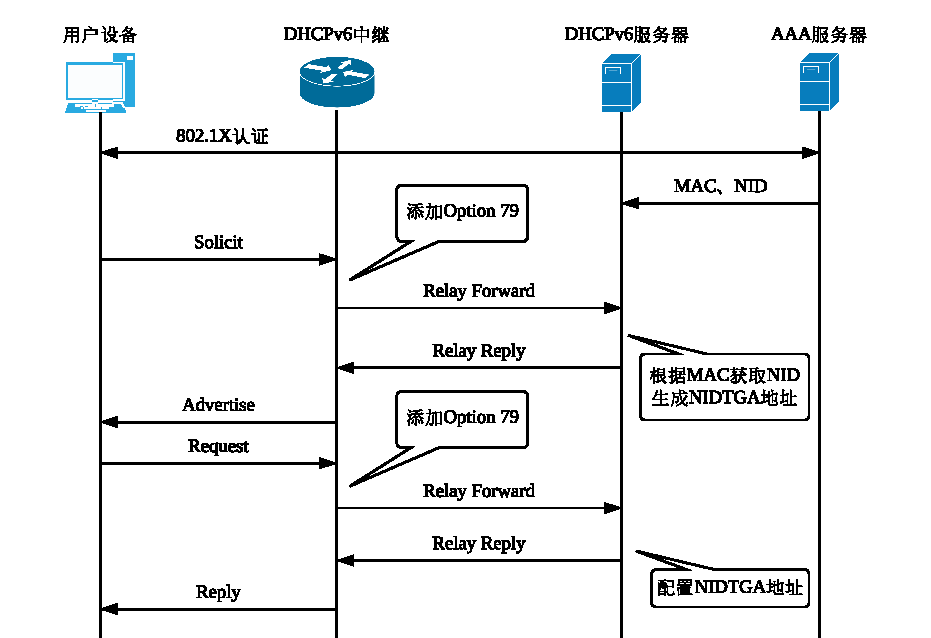
\includegraphics[width=0.9\textwidth]{DHCPv6_8021X_client.pdf}
      \caption{DHCPv6下802.1X认证的用户身份识别与溯源系统时序}
      \label{fig:DHCPv6_802.1X_client}
    \end{figure}


    \subsection{三种系统设计方案的实现部署情况}
    \label{NIDTGA:DHCPv6:implement}

        \subsubsection{基于扩展DHCPv6认证的系统设计方案}
        \label{NIDTGA:DHCPv6:implement:custom}
        目前,基于扩展DHCPv6认证的系统设计方案已经开发完成,在清华大学、北京大学、北京邮电大学、上海交通大学与东南大学五所高校进行了部署,并通过了288项目的验收。系统中主要包含以下几个部分,本文作者开发并重构了其中地址生成系统的代码与Windows客户端的代码,其他部分的代码主要由赛尔网络公司开发完成:
        \begin{enumerate}[1{)}]
          \item \textbf{用户注册系统}:如图\ref{fig:user_register_system}所示,包括用户登录与注册等功能,师生们填写真实信息后完成系统注册,获得用户身份标识NID。
            \begin{figure}[ht]
              \centering
              \subcaptionbox{登录页面\label{fig:user_register_system_0}}
              {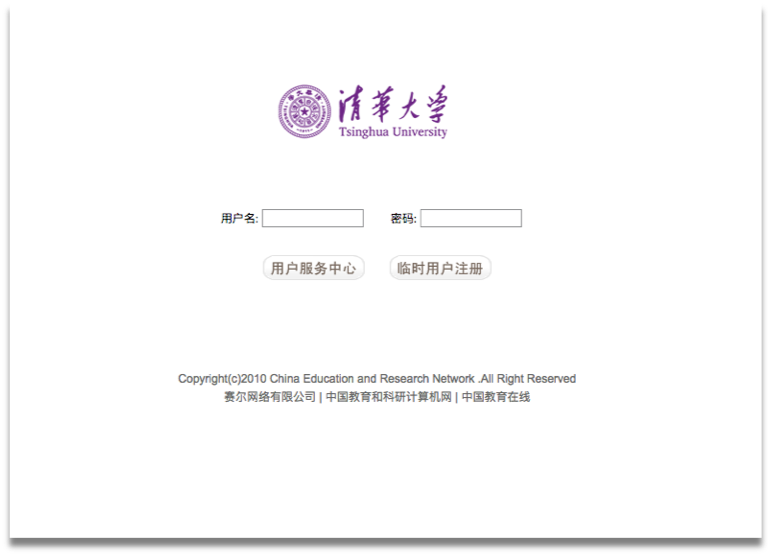
\includegraphics[height=4cm]{user_register_system_0.png}}
              \hspace{2em}
              \subcaptionbox{注册页面\label{fig:user_register_system_1}}
              {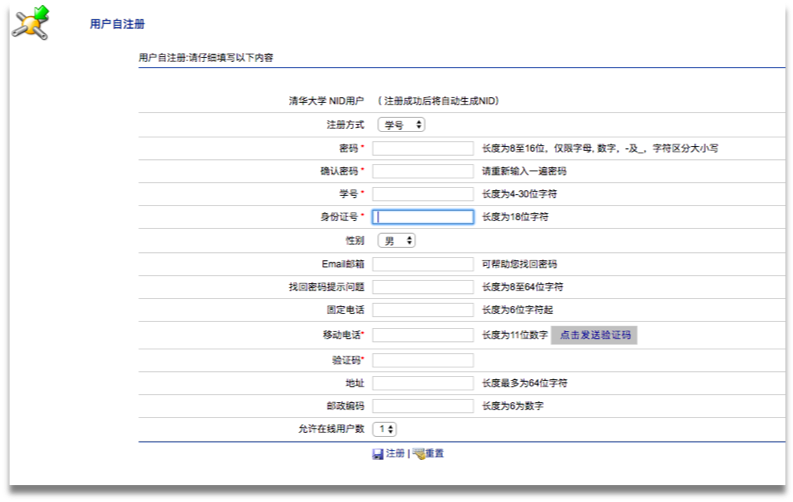
\includegraphics[height=4cm]{user_register_system_1.png}}
              \caption{288项目用户注册系统}
              \label{fig:user_register_system}
            \end{figure}
          \item \textbf{定制DHCPv6客户端}:客户端采用C\#进行实现,需要用户在设备上进行安装,用于连接系统后的认证,其将关闭操作系统内核的DHCPv6模块,启用自身的DHCPv6客户端功能进行IPv6地址请求,并配置设备网卡。Windows7/10、MacOS、Linux与Android系统下的客户端均已实现支持,其界面如图\ref{fig:user_custom_client}所示。
            \begin{figure}[ht]
              \centering
              \subcaptionbox{用户登录界面\label{fig:user_custom_client_0}}
              {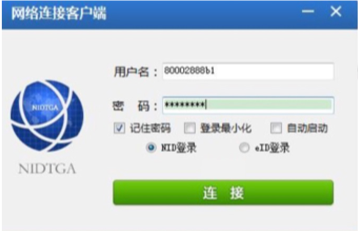
\includegraphics[height=4cm]{user_custom_client_0.png}}
              \hspace{2em}
              \subcaptionbox{认证成功界面\label{fig:user_custom_client_1}}
              {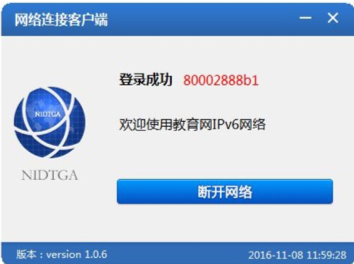
\includegraphics[height=4cm]{user_custom_client_1.png}}
              \caption{288项目用户DHCPv6客户端}
              \label{fig:user_custom_client}
            \end{figure}
          \item \textbf{地址生成系统}:地址生成系统基于ISC DHCP\footnote{ISC DHCP, https://www.isc.org/dhcp/}服务器的开源代码进行开发,主要以其server/dhcpv6.c中void dhcpv6(struct packet *packet)函数为入口,实现了NIDTGA地址的生成方案,修改了其IPv6地址配置的逻辑如图\ref{fig:custom_client_DHCPv6_server_logic}所示,以支持用户认证。
            \begin{figure}[ht]
              \centering
              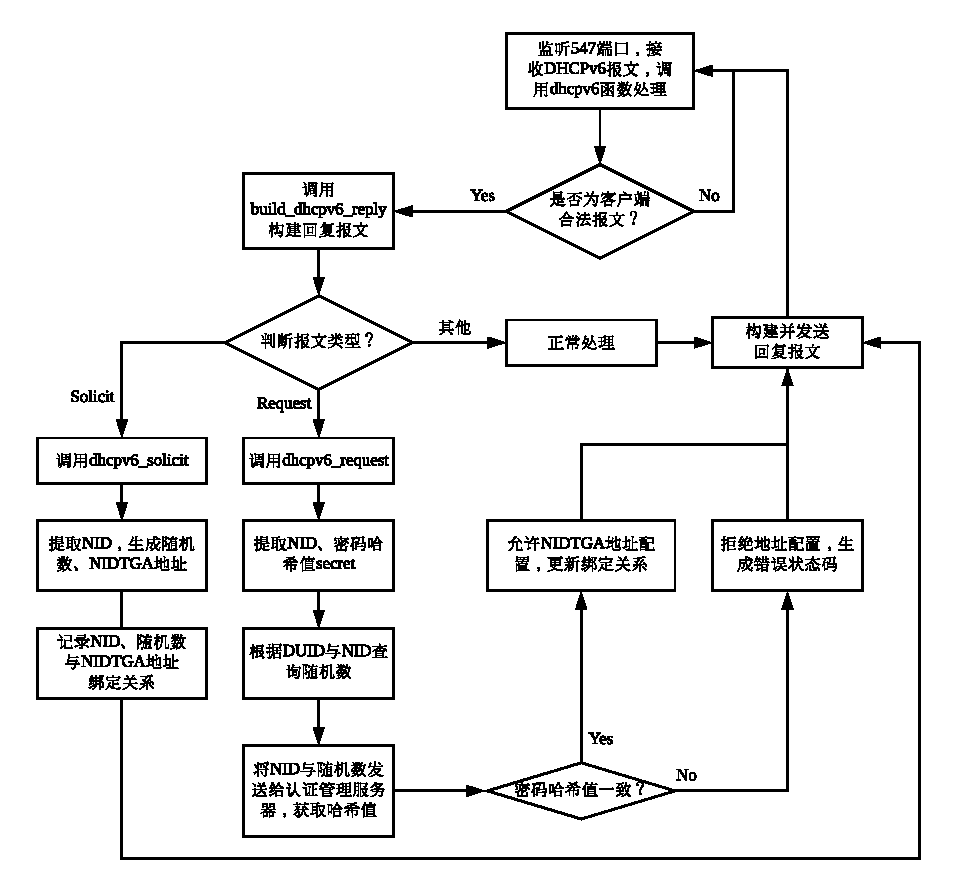
\includegraphics[width=0.9\textwidth]{custom_client_DHCPv6_server_logic.pdf}
              \caption{扩展DHCPv6认证的地址生成系统处理逻辑}
              \label{fig:custom_client_DHCPv6_server_logic}
            \end{figure}
          
          \item \textbf{网络管理系统}:网络管理系统可查看当前网络中的在线用户、SAVI交换机绑定表信息、以及整个系统中的用户注册数量等,如图\ref{fig:DHCPv6_client_deploy_result}所示,五所部署该系统的高校均包含4000以上的注册用户,整个系统的用户数量共计2万人以上。
            \begin{figure}[ht]
              \centering
              \subcaptionbox{清华大学部署情况\label{fig:DHCPv6_client_deploy_Tsinghua}}
              {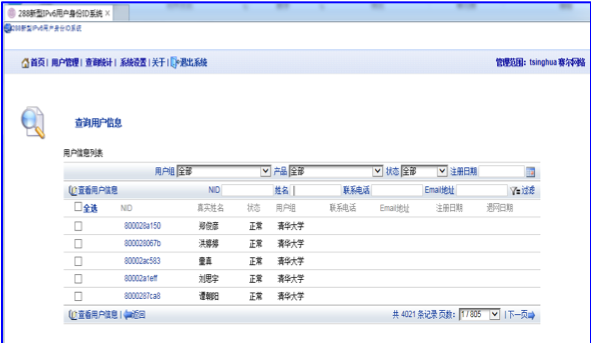
\includegraphics[height=4cm]{DHCPv6_client_deploy_Tsinghua.png}}
              \subcaptionbox{北京大学部署情况\label{fig:DHCPv6_client_deploy_Peking}}
              {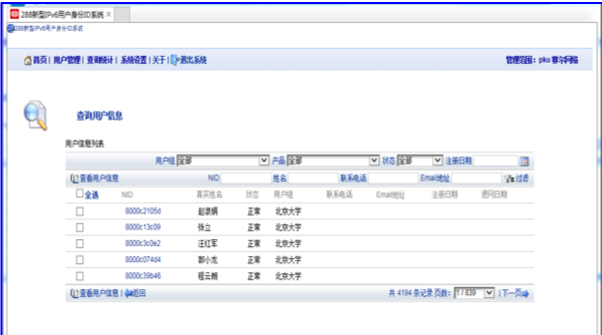
\includegraphics[height=4cm]{DHCPv6_client_deploy_Peking.png}}
              \caption{288项目高校部署情况举例}
              \label{fig:DHCPv6_client_deploy_result}
            \end{figure}
          \item \textbf{身份溯源系统}:身份溯源系统根据IPv6地址溯源用户身份信息,如图\ref{fig:user_trace_system}所示,为保护用户隐私,本文已将用户相关信息从图中抹去。
            \begin{figure}[ht]
              \centering
              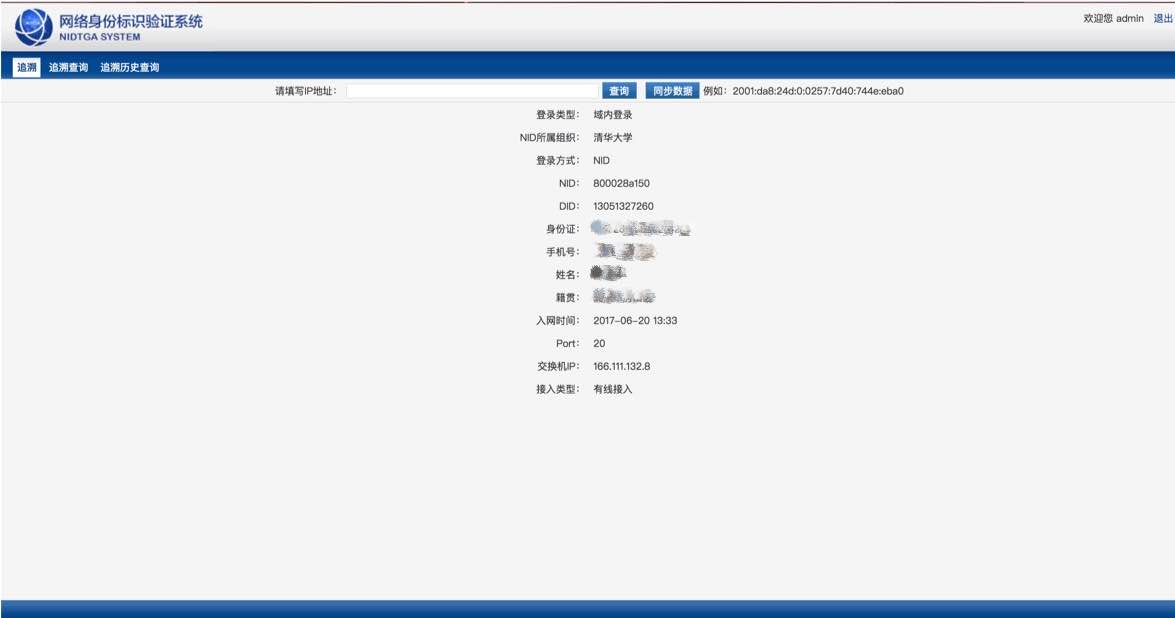
\includegraphics[height=6cm]{user_trace_system.jpeg}
              \caption{288项目身份溯源系统}
              \label{fig:user_trace_system}
            \end{figure}
        \end{enumerate}
    
        \subsubsection{基于Web Portal认证的系统设计方案}
        \label{NIDTGA:DHCPv6:implement:portal}
        基于Web Portal认证的方案已由本文作者独立进行原型系统的实现和验证,系统实现架构如图\ref{fig:DHCPv6_web_portal_implementation}所示。
        \begin{figure}[ht]
          \centering
          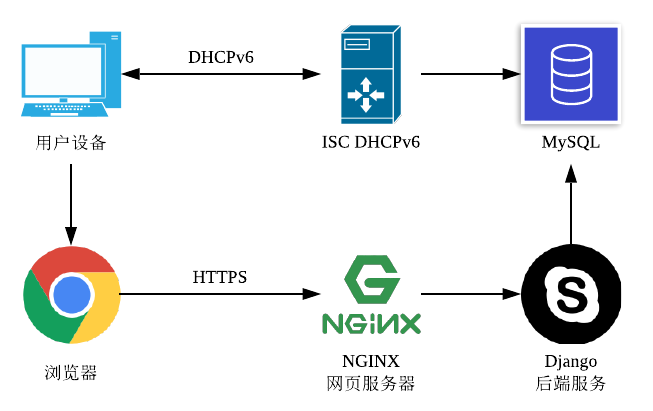
\includegraphics[width=0.6\textwidth]{figures/DHCPv6_web_portal_implementation.png}
          \caption{Web Portal认证的系统实现架构示意}
          \label{fig:DHCPv6_web_portal_implementation}
        \end{figure}
        
        系统主要包含两个部分:
        \begin{enumerate}[1{)}]
            \item \textbf{Web Portal认证系统}:Web Portal认证系统主要为用户提供Web Portal认证的网页服务,并向地址生成系统传递完成认证的用户相关信息。本文采用Django框架\footnote{Django, https://www.djangoproject.com/}开发了Web Portal网站,以MySQL\footnote{MySQL, https://www.mysql.com/cn/}作为用户认证数据库、以Nginx\footnote{Nginx, https://www.nginx.com/}作为网页服务器对其进行了部署测试。其逻辑较为简单,在用户访问时返回认证的HTML页面,在用户提交NID与密码认证后,查询数据库进行比对,返回提示认证成功与否的消息,并将NID、用户IPv6地址、认证时间写入数据库。
            \item \textbf{地址生成系统}:地址生成系统采用基于ISC DHCP服务器的开源代码扩展实现。在DHCPv6服务器配置文件中需要配置两个IPv6地址段,分别作为临时地址与NIDTGA生成地址。代码同样以对其中server/dhcpv6.c中void dhcpv6(struct packet *packet)函数为入口的执行逻辑修改为主,实现了图\ref{fig:web_portal_DHCPv6_server_logic}的过程。
            \begin{figure}[ht]
              \centering
              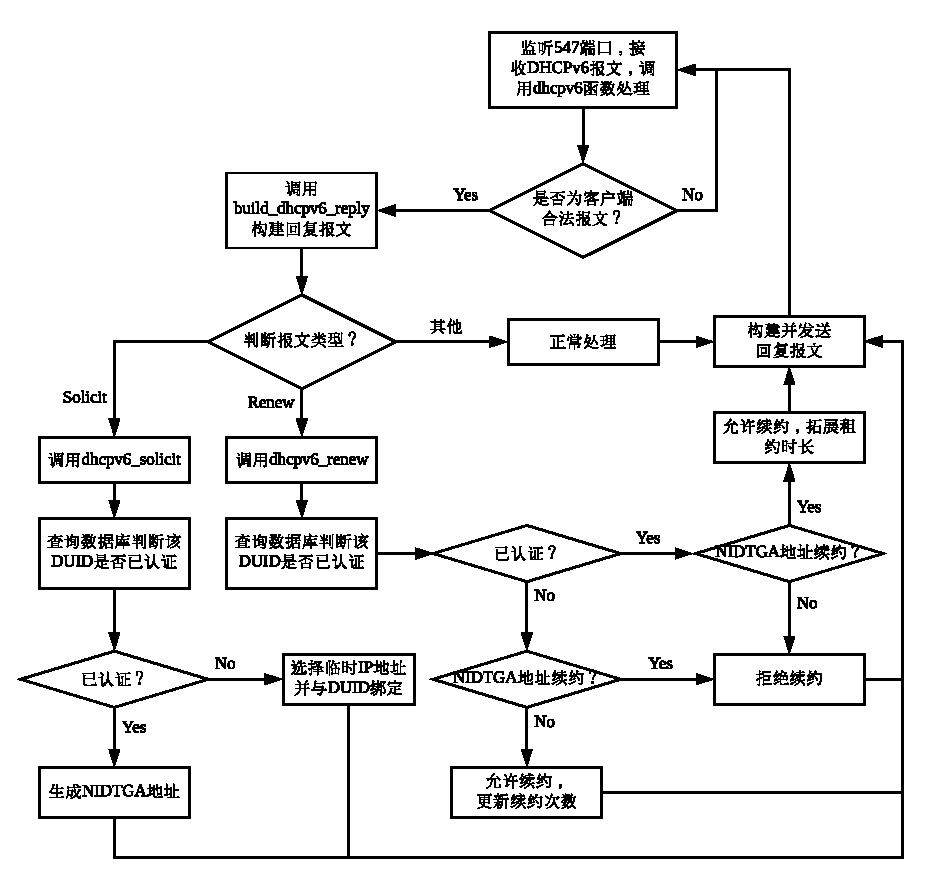
\includegraphics[width=0.9\textwidth]{web_portal_DHCPv6_server_logic.pdf}
              \caption{Web Portal认证的地址生成系统处理逻辑}
              \label{fig:web_portal_DHCPv6_server_logic}
            \end{figure}
        \end{enumerate}
    
        由于其存在较大的性能开销、用户等待延迟等问题,目前未在高校进行推广部署。

        \subsubsection{基于二层准入认证的系统设计方案}
        \label{NIDTGA:DHCPv6:implement:8021X}
        基于二层准入认证方案已由本文作者负责并与清华大学下一代互联网国家重点实验室的工程师合作实现,其实现架构如图\ref{fig:DHCPv6_8021X_implementation}所示。
        
        \begin{figure}[ht]
          \centering
          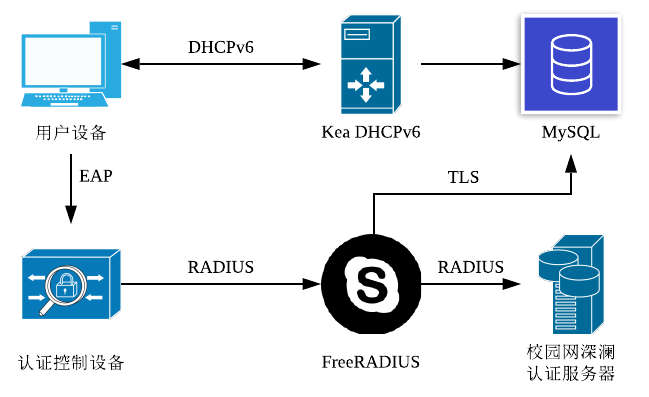
\includegraphics[width=0.6\textwidth]{figures/DHCPv6_8021X_implementation.png}
          \caption{二层准入认证的系统实现架构示意}
          \label{fig:DHCPv6_8021X_implementation}
        \end{figure}
        
        系统主要包含以下两个部分:
        \begin{enumerate}[1{)}]
          \item \textbf{地址生成系统}:基于Kea DHCP\footnote{Kea DHCP, https://www.isc.org/kea/}服务器的开源代码实现,主要包含Hook客户端与独立开发的地址生成服务。Kea DHCPv6服务器在处理用户地址配置请求报文时,使用扩展的Hook作为客户端与地址生成服务进行通信,获取NIDTGA地址,两者关系如图\ref{fig:user_address_generation_system}所示。DHCPv6服务器处的处理逻辑基本保持不变,将选择IPv6地址的过程更改为通过Hook向地址生成服务请求地址。地址生成服务监听传输层7839端口,与Hook建立socket通信,接收MAC地址,查询设备认证信息获得该设备的用户NID,为其生成NIDTGA地址并回复DHCPv6服务器。
            \begin{figure}[ht]
              \centering
              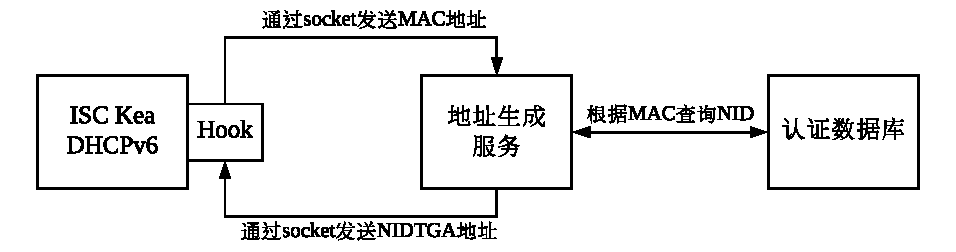
\includegraphics[width=0.9\textwidth]{user_address_generation_system.pdf}
              \caption{二层准入认证的地址生成系统构成示意}
              \label{fig:user_address_generation_system}
            \end{figure}
          \item \textbf{用户认证系统}:基于FreeRADIUS服务器的开源代码实现。为了增强系统部署推广能力,避免用户注册,支持校园网用户使用校园网账号认证,实现用户无感知接入,用户认证系统自动根据用户的校园网账号为其生成用户身份标识NID,并与校园网认证系统进行对接,自身作为RADIUS代理将用户认证请求通过RADIUS报文转发给校园网认证系统,在本地不存储用户密码相关的信息,以实现更好的安全性。
        \end{enumerate}
    
        \begin{figure}[ht]
          \centering
          \subcaptionbox{802.1X认证页面}
          {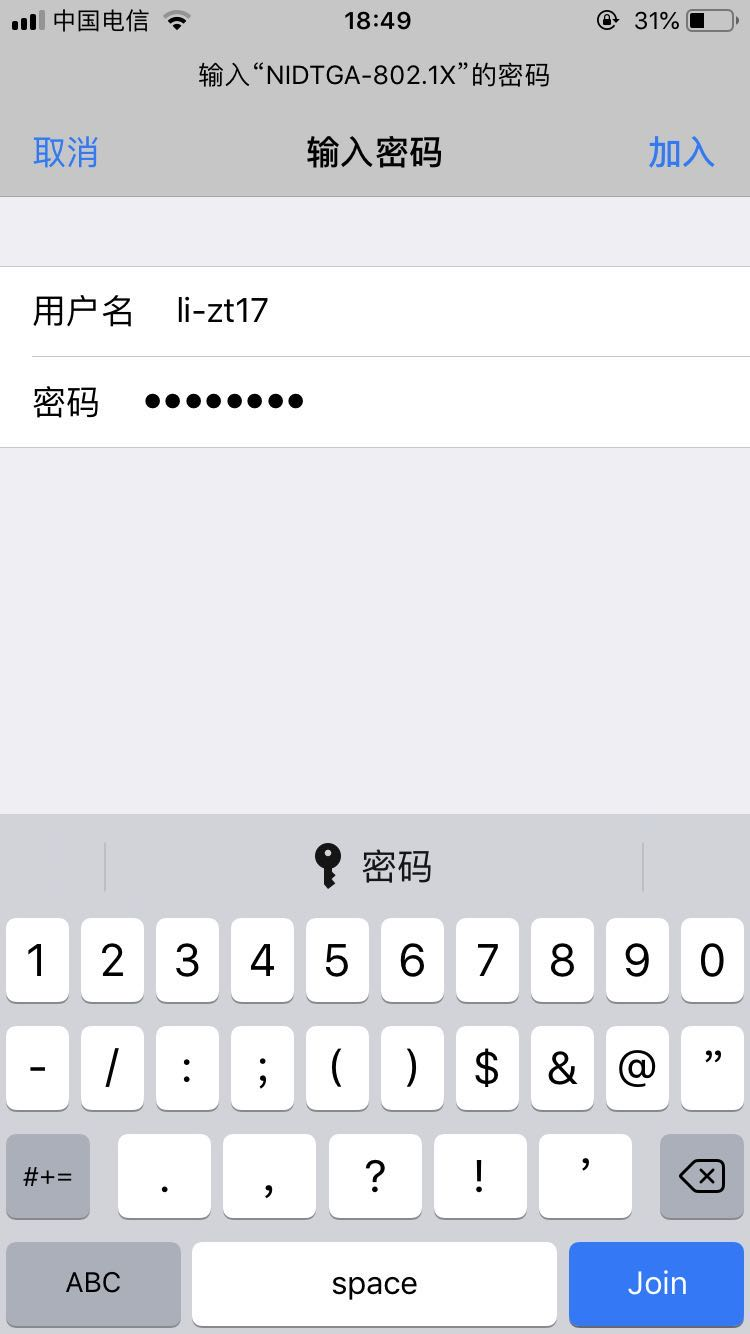
\includegraphics[height=6cm]{DHCPv6_8021X_deploy_0.jpeg}}
          \hspace{2em}
          \subcaptionbox{WiFi连接页面}
          {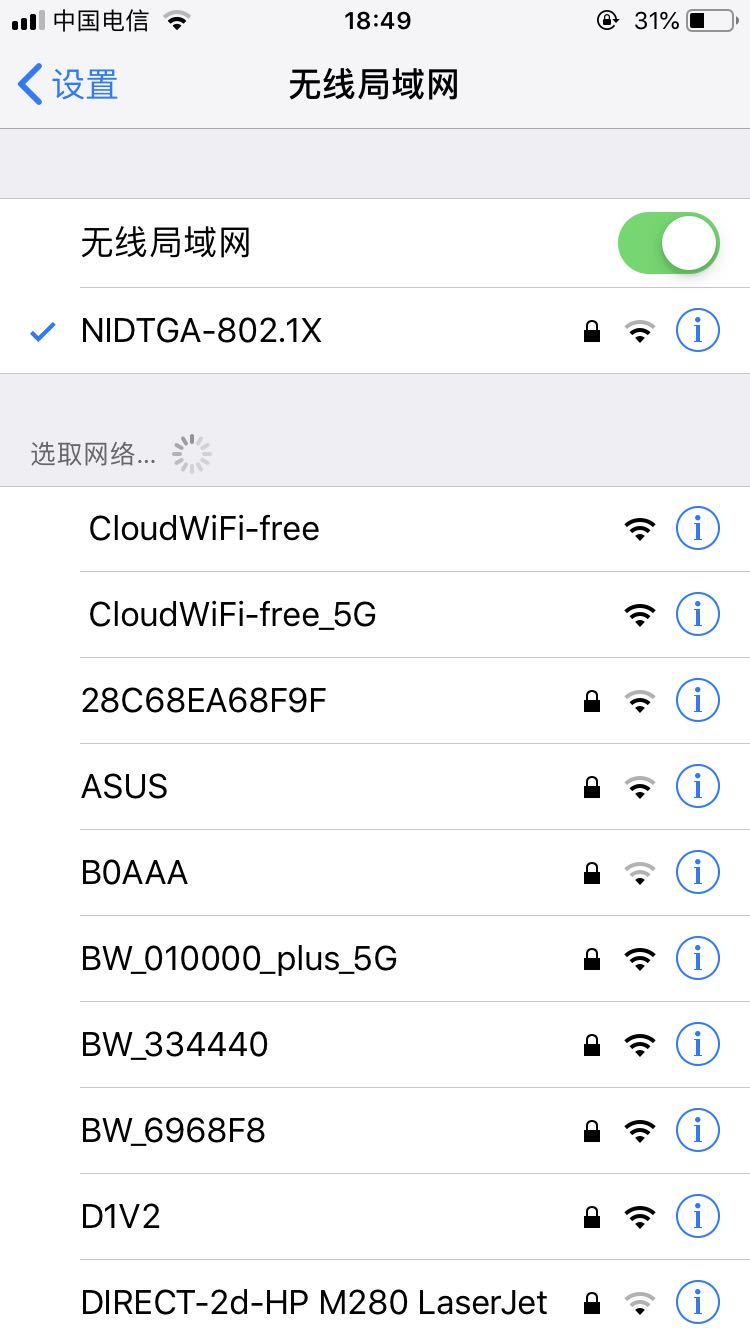
\includegraphics[height=6cm]{DHCPv6_8021X_deploy_1.jpeg}}
          \hspace{2em}
          \subcaptionbox{地址配置页面}
          {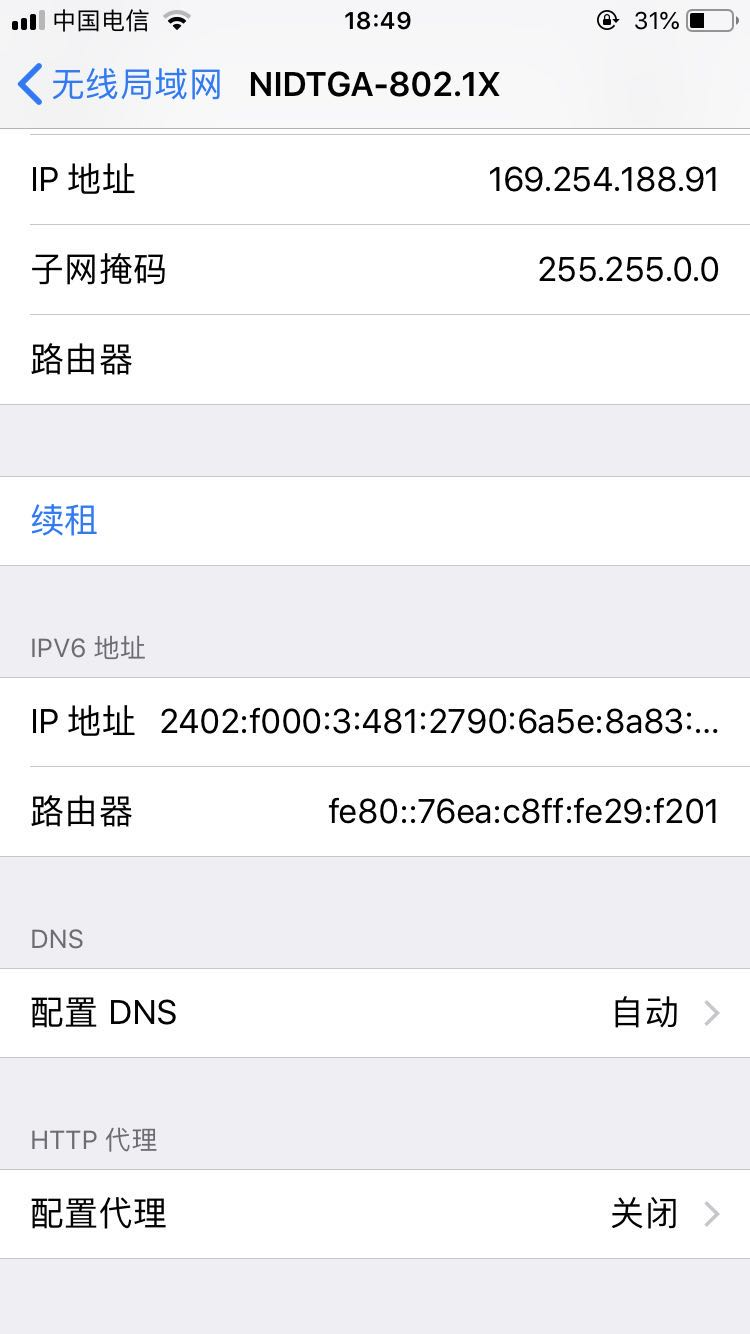
\includegraphics[height=6cm]{DHCPv6_8021X_deploy_2.jpeg}}
          \caption{清华大学二层准入认证系统部署用户认证举例}
          \label{fig:DHCPv6_8021X_deploy_result}
        \end{figure}
    
        目前,系统已在清华大学校园网中进行了部署与测试,在清华大学FIT楼104、204、229等房间的无线网络信号中有一个名为“NIDTGA-802.1X”的SSID。清华大学的师生连接该SSID后使用学校用户密码即可认证并访问网络。图\ref{fig:DHCPv6_8021X_deploy_result}所示为本文作者在iPhone手机上使用清华大学学生账号的用户名与密码连接“NIDTGA-802.1X”的页面举例,从第三张图中可以看到成功配置了一个由NIDTGA地址生成方案生成的IPv6地址。

    
    \subsection{三种系统设计方案的分析与对比}
    \label{NIDTGA:DHCPv6:comparison}
    在国家十三五重点研发项目“地址驱动的网络安全管控体系结构及其机理研究”中,DHCPv6下的用户身份识别与溯源系统将作为一项基础技术与应用示范在CNGI-CERNET2所连接的全国41所学校进行推广部署。本文在此分析各种认证方式下系统设计方案的优缺点,选择最适宜推广部署的方案总结在实际网络环境中的部署指南。
    
    三种方案在对用户设备、网络设备、系统实现等方面有着各自不同的要求,本文在此总结如下:
    \begin{enumerate}[1{)}]
      \item \textbf{扩展DHCPv6认证方案}:扩展DHCPv6认证方案需要禁用用户设备自身操作系统内核的DHCPv6客户端,使用自定义的DHCPv6客户端进行地址请求与配置,这种方式虽然可以支持一些暂不支持DHCPv6的操作系统,比如Android、Chrome OS等设备,但由于目前市场上操作系统繁杂,不同操作系统的系统调用接口均不同,同一操作系统的不同版本之间也存在差异,为了实现对用户设备的广泛支持,需要对每种操作系统进行针对性的客户端开发和维护,工作量巨大。对于Android等设备,安装定制DHCPv6客户端也需要用户拥有root权限,对用户并不友好。并且,采用扩展DHCPv6认证的方式,其认证过程与地址请求过程相耦合,虽然在本文的方案设计中采用了随机数的机制设计保护用户信息,但DHCPv6协议的安全问题仍会导致用户信息泄露、地址请求被假冒等问题。同时,在无线环境中,扩展DHCPv6认证手段本身无法保证用户认证后MAC地址不发生伪造,因此为了实现无线SAVI技术\cite{I-D.bi-savi-wlan},必须在网络中启用802.11i\cite{IEEE80211i}对MAC地址进行保护。在不使用802.1X认证的情况下,802.11i要求用户在接入网络时填写加密协商通信密钥过程的主密钥,这步密钥填写与用户采用定制的DHCPv6客户端的用户密码不同,可能令用户造成一定的困惑。
      \item \textbf{Web Portal认证方案}:Web Portal认证方案采用了轻量级的用户认证方式,用户设备无需安装任何客户端,使用浏览器即可以进行认证。其认证与地址配置流程均使用较为通用和标准化的技术,仅要求网络中接入控制设备具备对Web Portal认证功能的支持,但是该方案在DHCPv6服务器侧逻辑复杂,需要维护临时IPv6地址池与NIDTGA地址池的状态,在用户侧需要不断对临时IPv6地址进行续约,一方面会导致用户认证成功到用户获取得到NIDTGA地址之间存在一定延迟,影响用户体验,另一方面向网络中发送了大量的Renew报文,当用户数量较多时将显著增加网络设备负担。同时,通过Web Portal认证的方式也存在用户密码密文被窃取、用户身份被监听等安全隐患,需要HTTPS等协议的配合才能实现一定程度的安全性。同样,由于Web Portal认证手段无法保证用户MAC地址真实,因此在无线网络中也需要采用802.11i的机制以支持无线SAVI技术的部署。
      \item \textbf{二层准入认证方案}:二层准入认证方案的用户认证与地址配置方案均采用已被标准化的技术,对用户设备没有特殊要求,不需要安装客户端,也没有IPv6地址重新配置的流程,对用户比较友好,在DHCPv6服务器侧的状态维护比较简单。认证过程采用802.1X技术,可以保障认证过程中通信的安全性,并且防止攻击者伪造MAC地址,为无线SAVI技术的部署提供支持。地址配置过程中采用标准DHCPv6协议,对网络设备负担小。但是,由于需要向DHCPv6服务器告知请求地址的设备的MAC地址,因此该方案需要第一跳DHCPv6中继设备(一般是子网网关)支持RFC 6939这一标准。
    \end{enumerate}

    本文将三种方案的异同点总结如表\ref{tab:DHCPv6_implimentation_compare}所示。可见,二层准入认证的用户身份识别与溯源方案更为安全,认证过程对用户更友好,且对网络设备没有性能负担,原生支持无线SAVI的部署,保证用户源IPv6地址真实,适合推广部署。
    \begin{table}[htb]
      \centering
      \begin{minipage}[t]{\linewidth} 
        \caption{用户身份识别与溯源系统三种设计方案对比}
        \label{tab:DHCPv6_implimentation_compare}
        \begin{tabularx}{\linewidth}{c>{\centering\arraybackslash}X>{\centering\arraybackslash}X>{\centering\arraybackslash}X}
          \toprule[1.5pt]
          {\heiti 系统设计方案} & {\heiti 扩展DHCPv6认证} & {\heiti Web Portal认证} & {\heiti 二层准入认证} \\\midrule[1pt]
          {\heiti 用户设备要求} & 安装定制客户端 & 无 & 无 \\ 
          {\heiti 接入设备要求} & 无 & 无 & 802.1X认证 \\ 
          {\heiti 网关设备要求} & 无 & Web Portal认证 & DHCPv6 Client Link-Layer Address选项 \\ 
          {\heiti 地址分配过程} & 扩展DHCPv6,一次分配 & 标准DHCPv6,二次分配 & 标准DHCPv6,一次分配 \\  
          {\heiti 地址安全} & 无线网络中需要增加802.11i防止MAC地址伪造 & 无线网络中需要增加802.11i防止MAC地址伪造 & 原生支持MAC地址真实 \\
          {\heiti 优点} & 用户认证与地址配置流程简单,租约管理容易,可以支持没有DHCPv6功能的设备 & 无需用户安装客户端 & 无需用户安装客户端,认证过程安全且对用户友好,地址配置流程简单,租约管理容易 \\ 
          {\heiti 缺点} & 用户需要安装定制客户端,客户端需适配各操作系统版本开发并定期升级维护;需要用户填写802.11i加密密钥,对用户不友好;认证过程不安全 & 地址配置流程复杂;用户地址获取存在延迟;网络设备压力大;对网关设备有支持Web Portal认证的特殊需求;无法支持没有DHCPv6功能的设备;需要用户填写802.11i加密密钥,对用户不友好 & 对网关设备有支持DHCPv6 RFC6939的特殊需求;无法支持没有DHCPv6功能的设备 \\ 
          \bottomrule[1.5pt]
        \end{tabularx}
      \end{minipage}
    \end{table}

    \subsection{二层准入认证系统的校园网部署方案}
    \label{NIDTGA:DHCPv6:deploy}
    \ref{NIDTGA:DHCPv6:comparison}节中比较了多种用户身份识别与溯源系统的设计方案,并分析指出了基于二层准入认证的方案最为安全且用户友好。在对其进行实现后,如何在实际网络环境中部署也是用户身份识别与溯源系统得到实际应用至关重要的一环。由于支持DHCPv6配置地址的设备既有通过无线网络连接的笔记本、非Android操作系统的手机等移动终端,也有通过有线网络连接的台式电脑、服务器等设备,因此本节以校园网络为例,分别对无线与有线的两种环境下的部署方案进行研究。

      \subsubsection{无线校园网}
      \label{NIDTGA:DHCPv6:deploy:wireless}
      在CNGI-CERNET2所连接的41所全国高等院校中,所有学校的无线网络主要组网方式均为基于无线控制器的架构,尽管这种架构下对于802.1X报文等来自用户的管理帧均统一发送到AC进行处理,但对于用户的数据帧存在两种不同的报文转发模式:
      \begin{enumerate}[1{)}]
        \item \textbf{本地转发}:数据报文到达AP后,无需经过AC,直接由AP转发至上层网络经由有线网关进行路由转发。
        \item \textbf{集中转发}:数据报文到达AP后,由AP进行封装,统一经过IP隧道到达AC,由AC解封装后进行路由转发。
      \end{enumerate}

      根据\ref{NIDTGA:DHCPv6:comparison}节的分析,二层准入认证的用户身份识别与溯源系统对网络设备的功能有所要求,需要在用户设备经过的第一跳DHCPv6中继处支持RFC 6939中定义的Client Link-Layer Address选项以在Relay Forward报文中携带用户设备MAC地址。在本地转发模式下,第一跳DHCPv6中继为有线网关设备,而在集中转发模式下,第一跳DHCPv6中继为AC所旁挂的核心路由器设备。此外,由于实现用户身份识别与溯源的前提是IPv6地址真实,因此必须保证用户获取NIDTGA地址后访问网络时所使用的地址确实为其获取的NIDTGA地址,而非用户随意伪造的IPv6地址,因此用户身份识别与溯源系统还要求部署区域必须采用SAVI技术。

      因此,设计两种转发模式下的部署要求如图\ref{fig:wireless_deploy_request}所示。本地转发时的配置如下:
      \begin{itemize}
        \item AC:为用户身份识别与溯源系统划分出独立的SSID,配置相应VLAN、本地转发模式;配置接入子网源地址验证的SAVI技术,开启DHCPv6 Snooping;配置802.1X的认证方式,并设置AAA服务器地址、与AAA服务器进行通信的密钥等信息。
        \item AP上连的有线网关:为部署用户身份识别与溯源系统的VLAN开启DHCPv6中继功能,设置DHCPv6服务器地址,开启DHCPv6 Client Link-Layer Address选项功能;配置RA报文,开启Managed位与Other位,关闭Autonomous位。有线网关根据组网方式的不同可能位于汇聚交换机或核心路由器上,图\ref{fig:wireless_deploy_request}中以汇聚交换机为有线网关示意。
      \end{itemize}

      集中转发模式下的部署要求如下:
      \begin{itemize}
        \item AC:为用户身份识别与溯源系统划分出独立的SSID,配置相应VLAN、集中转发模式;配置SAVI,开启DHCPv6 Snooping;配置802.1X的认证方式,并设置AAA服务器地址、与AAA服务器进行通信的密钥等信息。
        \item AC所旁挂的核心路由器:为部署用户身份识别与溯源系统的VLAN开启DHCPv6中继功能,设置DHCPv6服务器地址,开启DHCPv6 Client Link-Layer Address选项功能;配置RA报文,开启Managed位与Other位,关闭Autonomous位。
      \end{itemize}

      \begin{figure}[ht]
        \centering
        \subcaptionbox{无线校园网部署拓扑\label{fig:wireless_deploy_request}}
        {\includegraphics[height=5cm]{wireless_deploy_request.pdf}}
        \hspace{2em}
        \subcaptionbox{有线校园网部署拓扑\label{fig:wired_deploy_request}}
        {\includegraphics[height=5cm]{wired_deploy_request.pdf}}
        \caption{校园网部署拓扑示意}
      \end{figure}

      \subsubsection{有线校园网}
      \label{NIDTGA:DHCPv6:deploy:wired}
      有线校园网络的典型拓扑较为简单,一般为用户设备连接在接入交换机上,接入交换机上连汇聚交换机,汇聚交换机再连接至校园网的核心路由器上。有线网关的位置根据管理方式的不同可能位于汇聚交换机上,也可能位于核心路由器上。其部署的要求如图\ref{fig:wired_deploy_request}所示:
      \begin{itemize}
        \item 接入交换机:对用户接入端口配置802.1X认证,设置AAA服务器地址、通信密钥等,并配置SAVI功能,开启DHCPv6 Snooping;
        \item 有线网关设备:为用户身份识别与溯源系统的部署区域划分VLAN;为部署的VLAN开启DHCPv6中继功能,设置DHCPv6服务器地址,开启DHCPv6 Client Link-Layer Address选项功能;配置RA报文,开启Managed与Other位,关闭Autonomous位。
      \end{itemize}

      \subsubsection{部署方案总结}
      \label{NIDTGA:DHCPv6:deploy:summary}
      由于各个高校的组网方式互相之间存在一些差异,尽管在前两小节对具有共性的组网方案进行了描述,但为了在实际推广部署时根据高校网络具体情况因地制宜提供指导,本文在此总结部署用户身份识别与溯源系统的需求框架。
      在无线网络与有线网络中进行部署时,有一些共同的要求:
      \begin{enumerate}[1{)}]
        \item \textbf{设备部署}:部署用户身份识别与溯源系统需要在校园网中添加技术相关的自研设备,包括采用NIDTGA地址生成方式的DHCPv6服务器、用户认证的AAA服务器,两个服务器均需要稳定的有线接入,配置静态的不发生变化的IPv6地址。
        \item \textbf{子网划分}:网络中需要划分部署用户身份识别与溯源系统的用户接入子网与部署系统控制设备的系统控制子网。每一个用户接入子网应独享一个/64的IPv6前缀,以确保用户设备可以正常获取和使用NIDTGA地址。系统控制子网需与用户接入子网保持独立,不与任何用户设备处于同一子网内,以确保用户设备发送的DHCPv6报文经过DHCPv6中继以携带Client Link-Layer Address选项。
      \end{enumerate}

      不论是有线环境还是无线环境,用户身份识别与溯源系统的部署对网络中已有设备的要求是一致的,只是根据组网方式的不同,DHCPv6中继与802.1X接入控制设备的位置在网络中会有所变化,本文将各种组网方式下行使各功能的网络设备与配置要求总结如表\ref{tab:DHCPv6_deploy_summary}所示。

      \begin{table}[htb]
        \centering
        \begin{minipage}[t]{\linewidth} 
          \caption{DHCPv6不同组网方式下的网络设备位置与配置要求总结}
          \label{tab:DHCPv6_deploy_summary}
          \begin{tabularx}{\linewidth}{>{\centering}m{2cm}>{\centering}m{1.8cm}>{\centering}m{1.8cm}>{\centering}m{1.8cm}>{\centering\arraybackslash}X}
            \toprule[1.5pt]
            \multirow{2}{*}{\heiti 设备功能} & \multicolumn{3}{c}{\heiti 组网方式} & \multirow{2}{*}{\heiti 配置要求} \\ 
            & {\heiti 无线网络本地转发} & {\heiti 无线网络集中转发} & {\heiti 有线网络} & \\\midrule[1pt]
            {\heiti 接入设备} & AP & AP & 接入交换机 & 开启SAVI,DHCPv6 Snooping \\ 
            {\heiti 802.1X接入控制设备} & AC & AC & 接入交换机 & 配置802.1X认证,设置AAA服务器地址与通信密钥  \\ 
            {\heiti DHCPv6中继} & 有线网关设备 & AC旁挂设备 & 有线网关设备 & 开启中继,设置DHCPv6服务器地址,开启Client Link-Layer Address选项功能  \\ 
            {\heiti 子网网关} & 汇聚交换机或核心路由器 & 核心路由器 & 汇聚交换机或核心路由器 & 划分VLAN,配置网关地址、IPv6前缀,开启路由器公告报文中Managed与Other位,关闭Autonomous位 \\
            \bottomrule[1.5pt]
          \end{tabularx}
        \end{minipage}
      \end{table}

  \section{SLAAC下的用户身份识别与溯源系统}
  \label{NIDTGA:SLAAC}
  尽管DHCPv6的地址配置方式更有利于组织管理员对用户上网进行控制和管理,但其地址配置流程比无状态地址配置SLAAC方式更为复杂,并且目前仍有设备的操作系统未实现DHCPv6协议,如Android系统、Chrome OS系统等,因此SLAAC方式仍是IPv6网络中一种重要的地址配置方式。

  但是,SLAAC方式由用户设备生成IPv6地址并进行重复地址检测,组织管理员无法控制用户如何生成和使用某一特定IPv6地址。同样,因为不能将IDEA密钥分发到用户端用于地址的生成,所以也不能通过类似于DHCPv6方式下定制客户端的方式实现。即便将密钥下发到用户端,也无法防止恶意用户使用错误的密钥或加密方式生成IPv6地址。

  SDN-Ti\cite{SDNTi}提出使用SDN对SLAAC地址配置方式下的用户IPv6地址进行映射,由SDN控制器为用户生成NIDTGA地址并下发映射规则给SDN交换机,SDN交换机负责将用户数据报文中的源IPv6地址替换为用户对应的NIDTGA地址再进行向外的转发,同时对以用户NIDTGA地址为目的地址的报文将其目的地址替换为用户设备的SLAAC地址后向内转发。SDN-Ti本质上是对用户使用SLAAC配置的IPv6地址进行了NAT,其虽然提出了SLAAC配置下实现用户身份识别与溯源系统的一种解决方案,但其在部署时需要将SDN交换机部署至每一个AP之上,SDN控制器也需要与AC协同工作处理所有的报文,这将极大地影响非通过用户身份识别与溯源系统接入的网络流量,容易造成网络的拥塞与不稳定,严重影响其他网络接入服务的可用性,其弊端大于配置NIDTGA地址的优势。

  因此,本文仍采用身份绑定的方式实现用户身份的溯源功能,作为覆盖暂未支持DHCPv6功能的设备的折中方案,而不将NID嵌入用户的IPv6地址中。

    \subsection{用户身份识别与溯源系统整体架构}
    \label{NIDTGA:SLAAC:architecture}
    本文设计的SLAAC地址配置方式下用户身份识别与溯源系统包含如图\ref{fig:SLAAC_system_architecture}所示的几个主要组成部分:
    \begin{enumerate}[1{)}]
      \item \textbf{认证控制设备}:网络中对用户接入进行认证控制的网络设备,一般为AC、接入交换机或宽带接入服务器等。用户所有流量均通过认证控制设备后才能进行跨子网的转发,认证控制设备将根据用户设备的认证情况,决定用户流量的转发策略。
      \item \textbf{SAVI设备}:监听用户设备地址配置控制报文的SAVI设备,将生成的IPv6地址与MAC地址等绑定表上报给认证管理服务器,一般部署于用户设备与认证控制设备之间,或者与认证控制设备一体。
      \item \textbf{认证管理服务器}:保存用户认证数据库的服务器。根据网络中认证手段的不同,具体形式将发生变化,在Web Portal认证方式下将包含Web Portal服务器与AAA服务器;在二层准入认证时为AAA服务器。
      \item \textbf{追溯服务器}:保存IPv6地址与用户身份绑定信息历史、提供用户身份溯源功能的服务器。根据网络中认证手段的不同,在Web Portal认证时其IPv6地址与用户身份绑定信息直接由认证管理服务器上传;在二层准入认证时需要将认证管理服务器上传的用户认证信息与SAVI设备上传的SAVI表项相结合,进行IPv6地址与用户身份绑定项的生成。
    \end{enumerate}

    \begin{figure}[ht]
      \centering
      \includegraphics[width=0.7\textwidth]{SLAAC_system_architecture.pdf}
      \caption{SLAAC下用户身份识别与溯源系统整体架构}
      \label{fig:SLAAC_system_architecture}
    \end{figure}

    在用户通过用户身份识别与溯源系统接入网络时,根据网络中配置的认证手段不同,在Web Portal认证下用户设备将先通过SLAAC配置地址再发起用户身份认证,在二层准入认证时则先完成用户身份认证而后配置IPv6地址。前者由于认证时设备已经配置了IPv6地址,因此可以较为简单地进行IP地址与用户身份的绑定;后者由于认证时设备尚未配置IPv6地址,因此本文提出了一种利用设备MAC地址标识设备、认证与SAVI技术相配合完成IPv6地址与用户身份绑定的设计方案。

    \subsection{基于Web Portal认证的系统设计}
    \label{NIDTGA:SLAAC:portal}
    在Web Portal认证的方式下,用户的NID与IPv6地址的关系可以在用户登录Web Portal认证的过程中比较容易地获取,其认证过程如图\ref{fig:SLAAC_web_portal}所示:
    \begin{enumerate}[1{)}]
      \item 网关向用户设备发送路由器公告RA报文,包含可配置的IPv6前缀等信息;
      \item 用户设备生成IPv6前缀下的IPv6地址后进行重复地址检测;
      \item 若用户设备在等待时间内未收到其他节点发来的对相同IPv6地址进行重复地址检测的NS报文或宣告持有该IPv6地址的邻居公告NA报文,则重复地址检测成功,设备为其网络接口配置该IPv6地址,并设定网关地址等信息;
      \item 用户使用浏览器访问网络,认证设备处还未有该IPv6地址的流量处理规则,因此被重定向至Web Portal网址;
      \item 用户提交NID与密码至Web Portal网站,Web Portal系统校验成功后,将用户NID与IPv6地址、认证时间信息上送给追溯服务器,并下发流量放行规则给认证控制设备;
      \item 认证控制设备允许用户数据报文正常转发;
      \item 用户手动访问Web Portal网站进行下线或认证控制设备检测到用户一段时间没有流量时,Web Portal认证系统向追溯服务器上传IPv6地址与下线时间。
    \end{enumerate}

    \begin{figure}[ht]
      \centering
      \includegraphics[width=0.9\textwidth]{SLAAC_web_portal.pdf}
      \caption{SLAAC下Web Portal认证的用户身份识别与溯源系统时序}
      \label{fig:SLAAC_web_portal}
    \end{figure}

    追溯服务器在收到Web Portal认证管理服务器上传的用户认证信息后,需要将NID、IPv6地址、时间等记录在数据库中,以供追溯使用,其表结构如\ref{tab:SLAAC_web_portal_binding}所示。
    \begin{table}[htb]
      \centering
      \begin{minipage}[t]{\linewidth} 
        \caption{SLAAC下Web Portal认证绑定关系数据表}
        \label{tab:SLAAC_web_portal_binding}
        \begin{tabularx}{\linewidth}{>{\centering\arraybackslash}X>{\centering\arraybackslash}X>{\centering\arraybackslash}X>{\centering\arraybackslash}X}
          \toprule[1.5pt]
          {\heiti 用户NID} & {\heiti IPv6地址} & {\heiti 上线时间} & {\heiti 下线时间}  \\\midrule[1pt]
          80002888b1 & 2402:f000:6:1c01: 6c28:70f1:be03:efe6 & 1583754484 & 1583758084 \\ 
          \multicolumn{4}{c}{...} \\
          \bottomrule[1.5pt]
        \end{tabularx}
      \end{minipage}
    \end{table}

    \subsection{基于二层准入认证的系统设计}
    \label{NIDTGA:SLAAC:8021X}
    在二层准入认证方式下,由于用户先使用链路层协议完成认证,后通过SLAAC配置IPv6地址,因此难以在用户认证时对用户NID与IPv6地址进行关联。考虑到用户身份识别与溯源系统所依赖的接入子网源地址验证技术SAVI能够监听SLAAC配置时的重复地址检测过程,并将无线网络中的信任锚MAC地址与IPv6地址进行绑定,而802.1X认证时同样以MAC地址标识不同的设备,因此我们可以采用MAC地址作为桥梁将用户NID与IPv6地址进行关联。

    本文在追溯服务器处维护已认证设备表与SAVI绑定表,分别如表\ref{tab:SLAAC_authorized_devices}与表\ref{tab:SLAAC_savi}所示,并根据两表通过算法\ref{algo:nid_ipv6_binding_table}生成用户身份与IPv6地址绑定表,如表\ref{tab:SLAAC_NID_IPv6_binding}所示。此外,追溯服务器还将生成已下线用户绑定表并写入数据库中,以支持对历史用户NID的查询。

    \begin{table}[htb]
      \centering
      \begin{minipage}[t]{\linewidth} 
        \caption{已认证设备表}
        \label{tab:SLAAC_authorized_devices}
        \begin{tabularx}{\linewidth}{>{\centering\arraybackslash}X>{\centering\arraybackslash}X>{\centering\arraybackslash}X}
          \toprule[1.5pt]
          {\heiti 设备MAC} & {\heiti 用户NID} & {\heiti 认证时间}  \\\midrule[1pt]
          78:31:c1:c8:10:8c & 80002888b1 & 1583754484 \\ 
          \multicolumn{3}{c}{...} \\
          \bottomrule[1.5pt]
        \end{tabularx}
      \end{minipage}
    \end{table}

    \begin{table}[htb]
      \centering
      \begin{minipage}[t]{\linewidth} 
        \caption{SAVI绑定表}
        \label{tab:SLAAC_savi}
        \begin{tabularx}{\linewidth}{>{\centering\arraybackslash}X>{\centering\arraybackslash}X>{\centering\arraybackslash}X}
          \toprule[1.5pt]
          {\heiti 设备MAC} & {\heiti AP} & {\heiti IPv6地址列表} \\\midrule[1pt]
          78:31:c1:c8:10:8c & 30-7B-AC-93-27-80: NIDTGA-802.1X & 2402:f000:6:1c01: 6c28:70f1:be03:efe6 \\ 
          \multicolumn{3}{c}{...} \\
          \bottomrule[1.5pt]
        \end{tabularx}
      \end{minipage}
    \end{table}

    \begin{table}[htb]
      \centering
      \begin{minipage}[t]{\linewidth} 
        \caption{在线用户绑定表}
        \label{tab:SLAAC_NID_IPv6_binding}
        \begin{tabularx}{\linewidth}{>{\centering\arraybackslash}X>{\centering\arraybackslash}X>{\centering\arraybackslash}X>{\centering\arraybackslash}X}
          \toprule[1.5pt]
          {\heiti 设备MAC} & {\heiti 用户NID} & {\heiti IPv6地址列表} & {\heiti 认证时间}\\\midrule[1pt]
          78:31:c1:c8:10:8c & 80002888b1 & 2402:f000:6:1c01: 6c28:70f1:be03:efe6 & 1583754484 \\ 
          \multicolumn{4}{c}{...} \\
          \bottomrule[1.5pt]
        \end{tabularx}
      \end{minipage}
    \end{table}

    其中表\ref{tab:SLAAC_authorized_devices}根据设备认证情况实时更新,每当有设备上线或下线时,AAA服务器将告知追溯服务器相应的用户NID与MAC地址信息,追溯服务器即将相应表项进行插入或删除。表\ref{tab:SLAAC_savi}则由认证控制设备在每当有新的SAVI绑定表项更新时上送给追溯服务器。

    \begin{algorithm}[ht]
      \caption{NID与IPv6地址绑定表生成算法}
      \label{algo:nid_ipv6_binding_table}
      
      \LinesNumbered
      \SetKw{KwInList}{in}
      \SetKw{KwBreak}{break}
      \KwIn{authorized\_device\_table, SAVI\_binding\_table}
      \KwOut{NID\_IPv6\_binding\_table}

      NID\_IPv6\_binding\_table \gets empty list\;
      \For{(MAC, NID, auth\_time) \KwInList authorized\_device\_table}{
        \For{(savi\_MAC, AP, IPv6\_list) \KwInList SAVI\_binding\_table}{
          \If{MAC $==$ savi\_MAC} {
            NID\_IPv6\_binding\_table.add((MAC, NID, IPv6\_list, auth\_time))\;
            \KwBreak\;
          }
        }
      }
    \end{algorithm}

    \begin{algorithm}[ht]
      \caption{已下线用户生成算法}
      \label{algo:nid_ipv6_logout_user}
      
      \LinesNumbered
      \SetKw{KwInList}{in}
      \SetKw{KwBreak}{break}
      \SetKw{KwTrue}{true}
      \SetKw{KwFalse}{false}
      \SetKw{KwAnd}{and}
      \KwIn{old\_NID\_IPv6\_binding\_table, new\_NID\_IPv6\_binding\_table}
      \KwOut{logout\_users}

      logout\_users \gets empty list\;
      \For{(old\_MAC, old\_NID, old\_IPv6\_list, old\_auth\_time) \KwInList old\_NID\_IPv6\_binding\_table}{
        is\_logout \gets \KwTrue\;
        \For{(new\_MAC, new\_NID, new\_IPv6\_list, new\_auth\_time) \KwInList new\_NID\_IPv6\_binding\_table}{
          \If{old\_NID $==$ new\_NID \KwAnd old\_IPv6\_list $==$ new\_IPv6\_list} {
            is\_logout \gets \KwFalse\;
            \KwBreak\;
          }
        }
        \If{is\_logout} {
          logout\_users.add((old\_MAC, old\_NID, old\_IPv6\_list, old\_auth\_time, current\_time))\;
        }
      }
    \end{algorithm}

    表\ref{tab:SLAAC_NID_IPv6_binding}将在表\ref{tab:SLAAC_authorized_devices}与表\ref{tab:SLAAC_savi}发生更新时调用算法\ref{algo:nid_ipv6_binding_table}进行更新。生成最新的在线用户绑定表后,与更新前的在线用户绑定表相比较,根据算法\ref{algo:nid_ipv6_logout_user}获得已下线用户绑定表并写入数据库中,其结构如表\ref{tab:SLAAC_NID_IPv6_logout_users}所示。

    \begin{table}[htb]
      \centering
      \begin{minipage}[t]{\linewidth} 
        \caption{已下线用户绑定表}
        \label{tab:SLAAC_NID_IPv6_logout_users}
        \begin{tabularx}{\linewidth}{>{\centering\arraybackslash}Xc>{\centering\arraybackslash}Xcc}
          \toprule[1.5pt]
          {\heiti 设备MAC} & {\heiti 用户NID} & {\heiti IPv6地址列表} & {\heiti 上线时间} & {\heiti 下线时间}\\\midrule[1pt]
          78:31:c1:c8:10:8c & 80002888b1 & 2402:f000:6:1c01: 6c28:70f1:be03:efe6 & 1583754484 & 1583758679 \\ 
          \multicolumn{5}{c}{...} \\
          \bottomrule[1.5pt]
        \end{tabularx}
      \end{minipage}
    \end{table}
    

    用户认证上线的交互时序如图\ref{fig:SLAAC_802.1X}所示,详细步骤不再赘述。

    \begin{figure}[ht]
      \centering
      \includegraphics[width=0.9\textwidth]{SLAAC_8021X.pdf}
      \caption{SLAAC下二层准入认证的用户身份识别与溯源系统时序}
      \label{fig:SLAAC_802.1X}
    \end{figure}

    当有用户追溯请求时,即可以IPv6地址为关键字向数据库中已下线用户绑定表查询绑定的用户NID信息。

    \subsection{两种系统设计方案的分析与对比}
    \label{NIDTGA:SLAAC:comparison}
    用户身份识别与溯源系统的这两种设计均是对SLAAC配置方式下无法控制IPv6地址生成这一困境的折中选择,在未来所有主流用户设备均支持DHCPv6地址配置时将逐步避免在SLAAC下部署用户身份识别与溯源系统方案。由于有线接入的用户设备基本均支持DHCPv6配置地址,因此这两种方案应主要考虑在无线场景下的部署,以对Android手机等设备进行支持。

    从身份与IPv6地址的绑定流程上来看,基于Web Portal认证的方式更为简洁,也是目前大多数未采用用户身份识别与溯源系统的网络中对用户身份进行管理所采用的方案,但其缺少对MAC地址安全性的保证,因而需要额外增加802.11i的机制来支持无线SAVI技术的部署,需要用户填写链路加密密钥的过程可能对用户产生困扰。

    与Web Portal认证的方案相比,二层准入认证的方案由于采用802.1X认证,提供了无线SAVI技术所要求的MAC地址安全性保证,因此能够预防恶意用户同时伪造MAC地址与IPv6地址的情况。同时,由于其二层认证的特性,追溯服务器能够在用户认证时获取到标识用户设备的MAC地址,为整个用户身份识别系统增加了更多拓展的可能。比如,虽然802.1X能够防止用户在认证成功后重新伪造MAC地址,但是对于恶意用户在认证前修改了其他用户的MAC进行认证这种行为,认证系统无法进行判断。而在二层准入认证方案的追溯服务器中,追溯服务器可以获得所有AC上送的全网的用户信息,因而能够检测到MAC地址冲突的情况,对于恶意用户修改他人MAC地址进行认证造成MAC地址冲突影响网络体验的行为,其可以采取一些黑名单的制度,告知认证控制设备对恶意用户进行下线处理,以惩戒恶意用户的攻击行为,在SAVI技术保障IPv6地址真实的基础上提供MAC地址真实性的保证。

    \subsection{系统实现情况与校园网部署方案}
    \label{NIDTGA:SLAAC:deploy}
    不论是Web Portal认证还是二层准入认证下的系统设计方案,其均需要与认证控制设备、SAVI设备等网络设备相配合进行实现,因此需要与具体的网络设备厂商进行合作。

    目前,考虑到对移动设备的漫游支持,基于二层准入认证并增加了MAC地址冲突检测的安全增强方案已与华为、新华三厂商分别合作进行了实现,并在清华大学无线网络中进行了大规模部署。两者的实现方案如图\ref{fig:Tsinghua_SAVI_implementation}所示。其中华为的Agile Controller与新华三的地址安全中心将记录全量的用户五元组信息绑定表并存储于清华大学大数据平台,在用户认证时提供全局的MAC地址、IPv6地址冲突校验功能,并与无线控制器进行通信将非法的用户设备进行下线处理。值得注意的是,两者的方案是建立在SAVI技术提供的源地址真实性基础上的源地址验证与溯源基础设施,其对MAC地址、IPv6地址进行冲突校验的功能不与IPv6地址配置方式耦合,因此同样适用于\ref{NIDTGA:DHCPv6:8021X}节中提出的系统设计方案,可为其提供MAC地址冲突校验的增强性保障。
    
    \begin{figure}[ht]
        \centering
        \subcaptionbox{华为IPv6源地址溯源方案\label{fig:Tsinghua_SAVI_huawei}}
        {\includegraphics[height=7cm]{figures/Tsinghua_SAVI_huawei.png}}
        \subcaptionbox{新华三IPv6源地址溯源方案\label{fig:Tsinghua_SAVI_h3c}}
        {\includegraphics[height=7cm]{figures/Tsinghua_SAVI_h3c.png}}
        \caption{SLAAC下用户身份识别与溯源系统的厂商实现与部署方案示意}
        \label{fig:Tsinghua_SAVI_implementation}
    \end{figure}

    由于用户身份识别与溯源系统在SLAAC下的设计方案均采用了被广泛应用或已标准化的认证技术与地址配置手段,用户身份与IPv6绑定都在服务器侧通过扩展功能实现,因此对于网络中的部署没有特殊的要求,各自采用传统的Web Portal认证与802.1X认证的部署方案即可。此外,同样需要网络设备采用SLAAC地址配置下的SAVI技术对用户伪造源IPv6地址的流量进行过滤,确保只有真实IPv6地址的流量才能够访问网络。本文将对各网络设备的要求总结如表\ref{tab:SLAAC_deploy_summary}所示。
    \begin{table}[htb]
      \centering
      \begin{minipage}[t]{\linewidth} 
        \caption{SLAAC下用户身份识别与溯源系统部署方案总结表}
        \label{tab:SLAAC_deploy_summary}
        \begin{tabularx}{\linewidth}{c>{\centering\arraybackslash}X>{\centering\arraybackslash}X}
          \toprule[1.5pt]
          {\heiti 系统设计方案} & {\heiti Web Portal认证} & {\heiti 二层准入认证}  \\\midrule[1pt]
          {\heiti 认证控制设备} & 宽带接入服务器或AC,开启Web Portal认证 & 接入交换机、宽带接入服务器或AC,开启802.1X认证 \\
          {\heiti 源地址验证设备} & 接入交换机或AC,开启SAVI功能、ND Snooping & 接入交换机或AC,开启SAVI功能、ND Snooping,定制向追溯服务器上传SAVI绑定表功能 \\ 
          {\heiti 认证授权设备} & AAA服务器,定制向追溯服务器上传NID与IPv6地址绑定表功能 & AAA服务器,定制向追溯服务器上传NID与MAC地址绑定表功能 \\
          \bottomrule[1.5pt]
        \end{tabularx}
      \end{minipage}
    \end{table}

  \section{静态配置下的用户身份识别与溯源系统}
  \label{NIDTGA:manual}
  静态配置地址一般用于机房或数据中心内部的设备配置,由设备负责人提出地址配置申请,组织管理员统一规划地址分配方案,并对各台接入设备进行手工配置。在未采用用户身份识别与溯源系统时,组织管理员将根据一定策略选择分配给用户的IPv6地址,比如采用与配置的IPv4地址一致的接口标识以便于IPv4与IPv6的统一管理。在采用用户身份识别与溯源系统时,组织管理员则需要将IPv6地址分配策略切换为使用NIDTGA方案生成地址的方式。

    \subsection{静态配置下的系统设计}
    \label{NIDTGA:manual:embed}
    本文将NIDTGA地址生成功能开放为一个工具供组织管理员使用。其生成地址所使用的IDEA密钥与DHCPv6下所使用的保持一致,以避免一个组织拥有两个不同的密钥更新历史。在为设备生成NIDTGA地址时,NIDTGA地址接口标识中嵌入的时间信息表示设备负责人申请静态地址的时间。

    当设备需要配置静态IPv6地址时,由设备的负责人向组织管理员提出申请,提交负责人的NID与所需要的IPv6地址数量、设备位置等信息。组织管理员根据设备位置确定设备接入子网的子网前缀,并根据负责人的NID与地址数量,使用NIDTGA地址生成工具根据算法\ref{algo:static_ipv6_generate}为其生成相应数量的地址。由于设备负责人提交的时间唯一而地址请求数量不唯一,因此算法\ref{algo:static_ipv6_generate}中以NIDTGA地址中时间信息的粒度NIDTGA\_TIME\_INTERVAL为步长,将生成的地址索引作为时间信息的变量,确保生成满足申请数目的不同的NIDTGA地址。

      \begin{algorithm}
        \caption{静态配置下NIDTGA地址生成算法}
        \label{algo:static_ipv6_generate}
        
        \LinesNumbered
        \SetKw{KwInList}{in}
        \SetKw{KwBreak}{break}
        \SetKw{KwTrue}{true}
        \SetKw{KwFalse}{false}
        \SetKw{KwAnd}{and}
        \KwIn{IPv6\_prefix, NID, address\_number}
        \KwOut{NIDTGA\_address\_list}

        NIDTGA\_address\_list \gets empty list\;
        current\_time \gets getEpochTime()\;
        \While{address\_number > 0}{
          NIDTGA\_address \gets IPv6\_prefix + encryptInterface(NID, current\_time + address\_number * NIDTGA\_TIME\_INTERVAL)\;
          NIDTGA\_address\_list.add(NIDTGA\_address)\;
          address\_number \gets address\_number - 1\;
        }
      \end{algorithm}

    \subsection{系统实现情况与校园网部署方案}
    \label{NIDTGA:manual:deploy}
    静态地址配置的用户认证识别与溯源系统以一个实现算法\ref{algo:static_ipv6_generate}的命令行工具为主,目前尚未在清华大学校园网内得到具体的应用。
    在静态配置地址的网络环境中部署用户身份识别与溯源系统,仅对设备获得的IPv6地址进行了干预,对网络配置与网络环境均没有发生任何干涉,所以在校园网部署时与传统的静态配置地址一致,没有特殊要求。设备配置静态地址后的入网行为需要由组织管理员采用配置接入控制列表等方式进行管理,建议在用户接入的第一跳交换机即配置相应的ACL表项以防止设备的地址伪造。

  \section{本章小结}
  \label{NIDTGA:summary}
  本章从实际网络环境中的IPv6地址配置方式出发,研究用户身份识别与溯源系统在各种场景下的设计、实现与部署。以与NIDTGA地址生成要求最契合的DHCPv6为重点,探讨和对比了三种不同的系统设计方式,并给出了二次准入认证的系统在校园网络中的部署方案,为用户身份识别与溯源系统的推广提供指引。同时也针对SLAAC与静态配置两种地址配置方式下的设计方案进行了研究,从而实现对所有设备接入场景的全面覆盖。各类系统设计方案目前均已完成了实现并得到了一定规模的部署,总结如图\ref{fig:system_implementation_status}所示。

  \begin{figure}[ht]
    \centering
    \includegraphics[width=\textwidth]{system_implementation_status.pdf}
    \caption{用户身份识别与溯源系统各种设计方案实现与部署情况}
    \label{fig:system_implementation_status}
  \end{figure}

% !TeX root = ../main.tex

\chapter{基于区块链的用户身份溯源系统}
\label{NIDTGA_Security}

  \section{本章引言}
  \label{NIDTGA_Security:introduction}
  用户身份识别与溯源系统的目标是为了根据IPv6地址追溯用户身份,形成用户上网行为的审计机制。因此,用户认证并获取NIDTGA地址是面向用户接入上网的基本功能,而根据NIDTGA地址追溯用户身份则是面向审计方对恶意用户身份进行溯源的目标功能。用户身份溯源的关键在于追溯服务器存储的组织密钥更新历史,在多组织部署的情形下,用户身份溯源系统将由一台全局唯一的追溯服务器统一存储各组织的密钥更新历史,以向审计方提供用户身份溯源服务。但是,一旦其遭到数据篡改或拒绝服务攻击,将导致系统用户身份溯源功能的失效,甚至泄露各组织的用户身份隐私,造成较大危害。
  
  本章首先分析多组织部署情况下的用户身份识别与溯源系统的设计,指出其中存在的中心化问题。然后利用区块链的去中心化与防数据篡改优势,研究使用区块链设计用户身份溯源系统的NIDChain方案,更好地保护组织密钥历史安全,提升用户身份溯源服务的可用性,并给出了NIDChain基于以太坊平台的原型实现与测试结果。

  本章内容组织如下:第\ref{NIDTGA_Security:analysis}节分析用户身份识别与溯源系统中各部分的安全性,阐述利用区块链构建用户身份溯源系统的动机;第\ref{NIDTGA_Security:design}节研究基于区块链的用户身份溯源系统设计方案NIDChain,包括审计方的追溯权限控制机制、区块中组织信息与密钥历史的数据结构、各管理域密钥更新机制等;第\ref{NIDTGA_Security:implement}节讨论了NIDChain基于以太坊平台的原型实现,给出其分布式应用与客户端的具体设计细节;第\ref{NIDTGA_Security:summary}节对本章研究内容进行总结。

  \section{用户身份识别与溯源系统的安全性分析}
  \label{NIDTGA_Security:analysis}

  用户身份识别与溯源系统的安全性包含用户认证上网与身份溯源两个部分。

  用户认证上网过程中涉及到的安全性问题有:
  \begin{itemize}
    \item \textbf{用户密码安全}:用户密码安全指的是用户的密码明文不会在认证过程中被其他用户获取,其安全性与具体认证方式有关。在扩展DHCPv6认证的实现方式中,我们设计了采用随机数与密码进行加密的方式保护用户密码明文;在Web Portal认证的实现中,可通过HTTPS协议来传递用户密码密文以提高安全性保障;在二次准入认证的实现方案中,802.1X认证方式要求用户设备与AAA服务器协商加密方法,因而可使用较高安全性的加密手段对用户密码进行加密传送。
    \item \textbf{用户身份安全}:用户身份安全是指用户的身份隐私是否能够得到良好的保护,即非审计方不应能够通过NIDTGA地址推断出用户的真实身份。在扩展DHCPv6认证的实现方式中,由于用户身份通过DHCPv6报文的扩展选项明文传输,链路内的恶意用户可以通过监听DHCPv6报文交互的过程,将用户NID与用户获得的NIDTGA地址关联起来,存在用户身份泄漏的安全隐患;在Web Portal认证的实现方式下,需要采用HTTPS协议对用户NID进行保护;在二层准入认证方式下,用户认证与地址配置流程解耦,且用户NID受到加密算法的保护,因此有着更高的安全性。同时,用户身份识别与溯源系统要求各组织定期更新用户生成NIDTGA地址的IDEA密钥,以确保不会有恶意攻击者收集到足够多的信息破解获得IDEA密钥从而获取用户身份。
    \item \textbf{用户地址安全}:用户地址安全是指用户的NIDTGA地址配置完成后,其地址不会被其他用户所盗用导致身份溯源时发生错误。在接入交换机与AC对SAVI源地址验证技术全部署的情况下,用户地址伪造无法发生,因而用户身份识别与溯源系统具有地址安全的特性。
  \end{itemize}

  用户身份溯源功能在系统多组织部署的情况下,由全局唯一的追溯服务器提供,各组织需要将生成NIDTGA地址用的IDEA密钥上传至追溯服务器进行保存,因此用户身份溯源功能涉及到的安全性问题包括以下几个方面:
  \begin{itemize}
    \item \textbf{追溯权限控制}:用户身份识别与溯源系统将部署该系统的各组织的密钥更新历史上传至全局追溯服务器,将用户身份进行追溯的权限开放给特定审计方。对于部署用户身份识别与溯源系统的各组织而言,他们拥有自身的IDEA密钥历史,因而自然可以追溯自己管理的用户身份,但其无法获取其他组织的密钥历史,因而无法追溯自身组织以外的用户身份。
    \item \textbf{密钥历史安全}:为了能够顺利追溯用户身份,用户身份识别与溯源系统要求追溯服务器中各组织的密钥历史准确无误。在各组织上传密钥过程中,可通过传输层安全性协议对应用层数据进行加密传输;在追溯服务器内部,需要保证其保存的各组织密钥历史数据不被篡改,但其本身没有提出任何安全防护与数据备份机制,面对数据篡改的攻击行为难以预防与恢复。
    \item \textbf{追溯功能可用}:追溯服务器作为一个集中式服务器,向审计方提供用户身份追溯服务。作为单一故障点,其服务面临可用性问题,极易受到分布式拒绝服务攻击,导致追溯功能不可用。
  \end{itemize}

  综上所述,通过选择合适的用户认证方式与数据传输协议,并配合良好部署的源地址验证技术,用户身份识别与溯源系统的现有设计可以保障用户认证过程中的安全,但在系统多组织部署的情况下,全局集中式的追溯服务器设计仍存在着数据易遭篡改与服务不可用的安全隐患。


  \section{基于区块链的用户身份溯源系统设计}
  \label{NIDTGA_Security:design}
  用户溯源系统的安全隐患主要来自于其追溯服务器的中心化设计。其中保存的各组织密钥历史数据容易受到篡改,其对审计方提供的服务容易受到DDoS攻击影响可用性。区块链作为具有防止数据篡改功能的分布式数据库,其天然具有保护数据安全并消除系统中单一故障点的能力,可以在攻击者未控制区块链网络中一半以上共识资源时持续形成共识提供服务,因此本文考虑使用区块链技术来建设用户身份识别与溯源系统中的追溯服务器,将其命名为NIDChain。

    \subsection{NIDChain整体设计}
    \label{NIDTGA_Security:design:architecture}
    用户身份识别与溯源系统中的追溯服务器支持的功能如下:
    \begin{enumerate}[1{)}]
      \item \textbf{组织信息更新}:当有新的组织部署用户身份识别与溯源系统时,其需要将用于部署该系统的相关信息提交给审计负责人进行维护,包括组织标识、组织名称、负责人姓名与联系方式、组织用户NID范围、生成NIDTGA地址的IPv6前缀等信息。
      \item \textbf{组织密钥更新}:各组织更新生成NIDTGA地址的IDEA密钥时,需要将新的密钥上传至追溯服务器以保证追溯服务器具有各组织的最新密钥历史,更新信息应包括组织标识、更新后的IDEA密钥、生效时间等信息。
      \item \textbf{用户身份追溯}:审计方使用追溯服务器开放的服务进行对某个NIDTGA地址对应用户NID的追溯,需要提交的信息为NIDTGA地址,追溯成功后向审计方提供用户NID、真实姓名、所属组织、上网时间等信息。
    \end{enumerate}

    在用户身份识别与溯源系统目前的设计实现中,组织信息更新功能由组织管理员在线下向审计方提交,并由审计方在追溯服务器中进行维护;组织密钥在DHCPv6服务器更新前通过TLS协议传递给追溯服务器,由追溯服务器将其记录在数据库中;用户身份追溯则由审计方向追溯服务器提交需要进行用户身份溯源的IPv6地址,追溯服务器查询数据库确定IPv6前缀所属组织后,根据组织密钥历史追溯获得用户NID,并向组织的用户身份管理服务器查询获得用户真实身份。

    在本文的设计中,原先多组织部署时中心化的追溯服务器转变为整个NIDChain的区块链网络,每个区块链节点都记录了原本集中式追溯服务器的全量信息,对于要写入NIDChain的信息,需要各个区块链节点根据共识算法对其进行共识,并将共识结果追加式地写入各自维护的区块链数据库中。每个组织可以拥有一个接入NIDChain的节点,以便组织管理员接入区块链网络。这一方面可以将NIDChain维持在一定规模,提升其安全性,另一方面使得每个组织均可以参与NIDChain中追溯信息的共识,消除额外的信任成本,增加用户身份识别与溯源系统的部署激励。其整体的设计架构如图\ref{fig:blockchain_nid_chain_architecture}所示,每个部署用户身份识别与溯源系统的组织维护一个区块链节点,加入到NIDChain网络中,组织管理员使用组织钱包通过客户端与NIDChain节点进行交互。审计方负责NIDChain的最初搭建与智能合约部署,其钱包的公私钥在控制用户身份追溯权限中有着特殊的作用。

    \begin{figure}[ht]
      \centering
      \includegraphics[width=\textwidth]{blockchain_nid_chain_architecture.png}
      \caption{NIDChain设计架构}
      \label{fig:blockchain_nid_chain_architecture}
    \end{figure}

    在建立NIDChain网络时,由审计方创建创世区块,并部署用于创建和维护组织信息的智能合约,本文将其命名为NIDAdmin。当有新的组织部署用户身份识别与溯源系统时,其启用一个新的区块链节点,连接进入NIDChain网络,同步区块链数据。组织管理员通过发布交易调用NIDAdmin,由NIDAdmin为该组织部署一个新的智能合约用于记录该组织的相关信息与密钥更新历史,本文将这类维护特定组织信息的智能合约命名为NIDOrg。

    本文设计NIDAdmin与NIDOrg中维护的信息分别如表\ref{tab:contract_NIDAdmin_information}与所示。其中OrgUpdateMsg为携带组织信息的结构体,其将在\ref{NIDTGA_Security:design:maintain}节中定义。KeyUpdateMsg为组织密钥更新消息的结构体,携带了组织历次密钥生成的密文与对应的生效时间,其设计为密文形式存储的原因将在\ref{NIDTGA_Security:design:authority}节说明。
    \begin{table}[htb]
      \centering
      \begin{minipage}[t]{\linewidth} 
        \caption{合约NIDAdmin信息列表}
        \label{tab:contract_NIDAdmin_information}
        \begin{tabularx}{\linewidth}{cc>{\centering\arraybackslash}X}
          \toprule[1.5pt]
          {\heiti 属性名} & {\heiti 类型} & {\heiti 说明} \\\midrule[1pt]
          public\_key & String & 审计方公钥 \\ 
          app\_queue & OrgUpdateMsg Array & 待审批的组织信息更新请求列表 \\ 
          org\_queue & NIDOrg Array & 记录组织信息的列表 \\
          \bottomrule[1.5pt]
        \end{tabularx}
      \end{minipage}
    \end{table}

    \begin{table}[htb]
      \centering
      \begin{minipage}[t]{\linewidth} 
        \caption{合约NIDOrg信息列表}
        \label{tab:contract_NIDOrg_information}
        \begin{tabularx}{\linewidth}{cc>{\centering\arraybackslash}X}
          \toprule[1.5pt]
          {\heiti 属性名} & {\heiti 类型} & {\heiti 说明} \\\midrule[1pt]
          org\_info & OrgUpdateMsg & 组织最新信息,包括组织名称、负责人联系方式、拥有的IPv6地址资源等 \\ 
          key\_history & KeyUpdateMsg Array & 组织密钥历史,以密钥密文与生效时间对的数组形式存储 \\ 
          \bottomrule[1.5pt]
        \end{tabularx}
      \end{minipage}
    \end{table}

    为了使与追溯功能相关的所有信息均记录在区块链上,以确保所有组织信息更新、密钥更新与用户追溯行为均可审计,因此本文将包括组织信息更新功能在内的所有能力,均通过智能合约NIDAdmin与NIDOrg提供给审计方或各个组织:
    \begin{enumerate}[1{)}]
      \item \textbf{组织信息更新}:组织信息更新实行由组织管理员提交申请、审计方进行批准的管理方式。组织管理员通过客户端连接区块链节点,使用本组织的私钥签发一条交易发布到NIDChain网络中,交易中包含对智能合约NIDAdmin的调用,完成申请的提交。审计方可通过区块链节点查看已有的申请,当需要批准或拒绝申请时,审计方使用自身私钥签发交易调用NIDAdmin的函数进行批准或拒绝。
      \item \textbf{组织密钥更新}:组织管理员使用客户端连接NIDChain节点,由客户端使用审计方的公钥将所要提交的新IDEA密钥加密后,与组织标识、密钥生效时间一起作为NIDOrg的输入,生成交易并使用本组织私钥签发后发布到NIDChain网络中。
      \item \textbf{用户身份追溯}:审计方连接区块链节点,调用NIDAdmin获取NIDTGA地址所属组织的密钥历史密文,审计方客户端利用私钥对密文进行解密,获取密钥明文历史,追溯获得用户NID,然后向用户组织的身份管理服务器查询用户真实身份。
    \end{enumerate}


    \subsection{追溯权限控制机制}
    \label{NIDTGA_Security:design:authority}
    数据公开透明是区块链的一个重要特点,由于每一个区块链节点都记录了完整的数据信息,因此写入区块链的任何数据对于区块链节点而言都是可见的。但是,对NIDTGA地址进行身份追溯的权限应该仅开放给审计方,避免不具有审计资格的人员能够根据NIDTGA地址追溯到其他组织内的用户身份,因此普通的组织管理员不应该能够获取得到其他组织的IDEA密钥明文历史。

    为了达成这个目的,在向区块链中写入组织更新的密钥时,必须对其进行加密,使得仅有审计方能够对密文进行解密。本文采用椭圆曲线算法\cite{koblitz1987elliptic,miller1985use}来解决这一问题,如图\ref{fig:NIDChain_key_update}所示。
    
    \begin{figure}[ht]
      \centering
      \includegraphics[width=\textwidth]{figures/NIDChain_key_update.png}
      \caption{NIDChain追溯权限控制机制示意}
      \label{fig:NIDChain_key_update}
    \end{figure}
    
    ECC算法使用的参数与区块链中钱包的公私钥对生成参数保持一致,以比特币采用的secp256k1\cite{qu1999sec}为例:
    \begin{enumerate}[1{)}]
      \item 组织管理员获取审计方公钥$public\_key$,采用secp256k1的参数设置对IDEA密钥$key$进行椭圆曲线加密,生成$encrypted\_key$。
      \item 审计方使用私钥$secret\_key$对$encrypted\_key$进行解密,获得明文$key$。其他组织的区块链节点虽然能够获得每个组织历次更新的$encrypted\_key$,但由于没有$secret\_key$,因而无法获得$key$。
    \end{enumerate}

    \subsection{组织信息更新机制}
    \label{NIDTGA_Security:design:maintain}
    组织信息更新发生在有新组织部署用户身份识别与溯源系统或已部署的组织变更其身份认证管理服务器信息与组织管理员等信息时,本文设计组织信息更新消息的结构如表\ref{tab:blockchain_design_organization_update_message}所示,将其命名为OrgUpdateMsg。
    \begin{table}[htb]
      \centering
      \begin{minipage}[t]{\linewidth} 
        \caption{组织信息更新消息OrgUpdateMsg格式}
        \label{tab:blockchain_design_organization_update_message}
        \begin{tabularx}{\linewidth}{cc>{\centering\arraybackslash}X>{\centering\arraybackslash}X}
          \toprule[1.5pt]
          {\heiti 属性名} & {\heiti 类型} & {\heiti 举例} & {\heiti 说明} \\\midrule[1pt]
          name & String & 张三 & 组织管理员姓名  \\ 
          phone & String & 13845678576 & 组织管理员电话 \\ 
          email & String & zs@tsinghua.edu.cn & 组织管理员邮箱 \\ 
          nid\_addr & String & 2402:f000:1:1011::1 & 组织用户身份管理服务器IPv6地址 \\ 
          port & Integer & 8888 & 供审计方通信的组织用户身份管理服务器传输层端口号 \\ 
          ipv6\_pool & String Array & [2402:f000:1:1001::, 2402:f000:1:1002::] & 组织用于生成NIDTGA地址的IPv6前缀列表 \\
          \bottomrule[1.5pt]
        \end{tabularx}
      \end{minipage}
    \end{table}

    组织在部署用户身份识别与溯源系统后,必须向NIDAdmin更新其组织信息。第一次更新组织信息被称为组织注册,NIDAdmin将以组织注册交易的发起地址作为唯一的组织标识,与记录该组织信息的NIDOrg合约相绑定,在后续组织信息更新时NIDAdmin将对其组织标识进行校验,要求更新组织信息的交易发起地址与对应的NIDOrg组织标识一致。OrgUpdateMsg中各属性在组织注册时必须提供合法的值,在后续的组织信息更新时可为空,NIDAdmin将认为其对应字段不修改。

    组织管理员填写组织信息更新消息后,经由客户端发起交易,调用智能合约NIDAdmin提供的组织信息更新函数,本文将其命名为orgUpdate。NIDChain收到该交易后进行共识,调用各自维护的NIDAdmin合约执行相关调用。orgUpdate操作执行成功后,组织的信息并未真正更新,而是被NIDAdmin添加到待审批列表app\_queue内。审计方将查看NIDAdmin的app\_queue,对组织的信息维护操作进行审批,通过调用NIDAdmin的updateApprove与updateReject函数分别批准或拒绝组织的信息维护,经过批准的组织信息将被更新到NIDAdmin内实际的组织列表org\_queue中。组织信息更新的时序如图\ref{fig:blockchain_organization_update_procedure}所示。

    \begin{figure}[ht]
      \centering
      \includegraphics[width=0.9\textwidth]{blockchain_organization_update_procedure.pdf}
      \caption{NID组织信息更新时序}
      \label{fig:blockchain_organization_update_procedure}
    \end{figure}

    智能合约NIDAdmin中将维护app\_queue与org\_queue两个列表,其中app\_queue记录了各组织管理员已提交但待审批的组织信息,org\_queue中记录了目前已部署用户身份识别与溯源系统的各组织的信息。审计方可通过查看app\_queue审批组织信息的更新申请,被批准的组织信息将根据其组织标识更新org\_queue中对应组织的信息。org\_queue中每一个组织状态均由一个智能合约NIDOrg维护,当组织标识不在org\_queue的列表中时,说明该组织为新部署用户身份识别与溯源系统,NIDAdmin将为其创建一个新的NIDOrg合约并加入org\_queue中。

    NIDAdmin为组织信息更新机制提供的相关函数总结如表\ref{tab:contract_organization_update_function}所示。

    \begin{table}[htb]
      \centering
      \begin{minipage}[t]{\linewidth} 
        \caption{NIDAdmin组织信息更新相关函数}
        \label{tab:contract_organization_update_function}
        \begin{tabularx}{\linewidth}{cc>{\centering\arraybackslash}Xc>{\centering\arraybackslash}X}
          \toprule[1.5pt]
          {\heiti 函数名} & {\heiti 参数类型} & {\heiti 返回类型} & {\heiti 调用者} & {\heiti 说明} \\\midrule[1pt]
          orgUpdate & OrgUpdateMsg & 无 & 组织管理员 & 接收组织信息更新请求,加入待审核列表 \\ 
          updateQuery & 无 & OrgUpdateMsg Array & 审计方 & 查询待审批的组织信息更新请求列表 \\ 
          updateApprove & String & 无 & 审计方 & 接收组织钱包地址,通过相应组织信息更新请求 \\ 
          updateReject & String & 无 & 审计方 & 接收组织钱包地址,拒绝相应组织信息更新请求 \\ 
          \bottomrule[1.5pt]
        \end{tabularx}
      \end{minipage}
    \end{table}


    \subsection{组织密钥更新机制}
    \label{NIDTGA_Security:design:update}
    组织密钥更新发生在组织管理员更新用于NIDTGA地址接口标识加密的IDEA密钥时。用户身份识别与溯源系统在更新本地DHCPv6服务器的密钥前,需要由组织管理员先向NIDChain提交组织密钥更新,以确保在DHCPv6服务器使用新的密钥生成地址时,审计方已经可以使用新密钥对最新地址进行追溯。本文称组织客户端向NIDChain网络提交的组织密钥更新消息为KeyUpdateMsg,包含两个属性,一个是encrypted\_key,由组织管理员填写,用于携带经过ECC加密后的IDEA密钥密文,另一个是effect\_time,在发起交易时由程序按照当前时间自动填充,用于携带密钥更新时间,如表\ref{tab:blockchain_design_key_update_message}所示。之所以需要在密钥更新消息中由客户端主动填充当前时间,而不使用实际更新区块链数据时的时间作为密钥生效时间,是由于区块链的数据更新对客户端而言是一个异步操作,其需要等待交易被打包进新的区块,并等待新区块在区块链网络中形成共识,在区块链运行智能合约的虚拟机内部难以获知现实时间的确切时间,其仅能通过区块的共识时间了解当前所处的时间区间,因此如果采用区块时间作为新密钥的生效时间,将导致记录的生效时间比实际生效时间严重滞后。

    \begin{table}[htb]
      \centering
      \begin{minipage}[t]{\linewidth} 
        \caption{组织密钥更新消息KeyUpdateMsg格式}
        \label{tab:blockchain_design_key_update_message}
        \begin{tabularx}{\linewidth}{cc>{\centering\arraybackslash}X>{\centering\arraybackslash}X}
          \toprule[1.5pt]
          {\heiti 名称} & {\heiti 类型} & {\heiti 举例} & {\heiti 说明} \\\midrule[1pt]
          encrypted\_key & String & b/zHpAdf+W1PgGW Wcw+LqBrvJ1lVhO nsIOzd+BkVi1JII Trionfx+gM90TaV 0uxDY6mqBgsN3z kXcyaMYRizOA== & IDEA密钥经过审计方公钥使用ECC加密后的密文 \\ 
          effect\_time & Integer & 1586916525 & 密钥生效时间 \\ 
          \bottomrule[1.5pt]
        \end{tabularx}
      \end{minipage}
    \end{table}

    当组织管理员通过客户端更新IDEA密钥时,客户端首先向NIDChain查询获取审计方公钥,通过ECC加密算法将新的IDEA密钥进行加密,形成KeyUpdateMsg后,签发交易调用智能合约NIDOrg提供的密钥更新函数keyUpdate,将新的密钥追加至其密钥历史key\_history的队尾。key\_history中每一条记录均记录了每次更新的密钥密文与生效时间。执行成功后,客户端再将IDEA密钥的明文通过TLS发送给本地的DHCPv6服务器进行更新。

    组织密钥更新机制中涉及的智能合约函数总结如表\ref{tab:contract_key_update_function}所示。
    \begin{table}[htb]
      \centering
      \begin{minipage}[t]{\linewidth} 
        \caption{NIDOrg组织密钥更新相关函数}
        \label{tab:contract_key_update_function}
        \begin{tabularx}{\linewidth}{c>{\centering\arraybackslash}Xcc>{\centering\arraybackslash}X}
          \toprule[1.5pt]
          {\heiti 函数名} & {\heiti 参数类型} & {\heiti 返回类型} & {\heiti 调用者} & {\heiti 说明} \\\midrule[1pt]
          keyUpdate & KeyUpdateMsg & 无 & 组织管理员 & 更新对应组织密钥历史 \\
          \bottomrule[1.5pt]
        \end{tabularx}
      \end{minipage}
    \end{table}
    
    \subsection{用户身份追溯机制}
    \label{NIDTGA_Security:design:trace}
    用户身份追溯由审计方发起,需要经历图\ref{fig:blockchain_nid_trace_procedure}所示过程:
    \begin{enumerate}[1{)}]
      \item \textbf{查询组织密钥历史}:审计方通过客户端以NIDTGA地址作为参数调用合约NIDAdmin,NIDAdmin根据NIDTGA地址的前缀,查询NIDOrg列表,确定其所属组织,将该组织的信息与密钥历史返回客户端。客户端使用审计方私钥,从组织密钥历史队尾开始逐个向前解密获得IDEA密钥明文,用于尝试解密NIDTGA地址的接口标识,获得用户NID与上网时间。
      \item \textbf{查询用户真实身份}:审计方将用户真实身份查询请求用私钥采用ECC算法签名后发送给该组织用户身份管理服务器,与用户身份管理服务器的通信信息由NIDOrg中的nid\_addr与port确定。用户身份管理服务器使用审计方公钥对数字签名进行验证后,答复NID对应用户的真实身份,答复同样将用户真实身份使用审计方公钥加密,以防止被攻击者窃听获取。
    \end{enumerate}

    \begin{figure}[ht]
      \centering
      \includegraphics[width=\textwidth]{blockchain_nid_trace_procedure.pdf}
      \caption{NIDChain用户真实身份追溯时序}
      \label{fig:blockchain_nid_trace_procedure}
    \end{figure}

    因此,本文设计NIDAdmin与NIDOrg提供用户组织查询的函数如表\ref{tab:contract_org_query_function}所示。
    \begin{table}[htb]
      \centering
      \begin{minipage}[t]{\linewidth} 
        \caption{用户组织查询相关函数}
        \label{tab:contract_org_query_function}
        \begin{tabularx}{\linewidth}{ccccc>{\centering\arraybackslash}X}
          \toprule[1.5pt]
          {\heiti 合约名} & {\heiti 函数名} & {\heiti 参数类型} & {\heiti 返回类型} & {\heiti 调用者} & {\heiti 说明} \\\midrule[1pt]
          NIDAdmin & orgQuery & String & NIDOrg & 审计方 & 接受NIDTGA地址作为参数,返回该地址所属组织的信息 \\ 
          NIDOrg & addrCheck & String & Boolean & NIDAdmin & 判断NIDTGA地址是否属于该组织,是则返回True \\ 
          \bottomrule[1.5pt]
        \end{tabularx}
      \end{minipage}
    \end{table}

    由于客户端在更新密钥时,由客户端填充密钥更新消息中的密钥生效时间,而后再更新本地生成NIDTGA地址的密钥,因此区块链中记录的密钥生效时间将一定程度早于密钥的实际生效时间,如图\ref{fig:key_valid_time_drift}中DELTA所示。DELTA包含的时间主要由两部分组成:客户端向DHCPv6服务器传输新密钥的时间和在将新密钥更新至DHCPv6服务器内存中的时间。前者需要建立TLS的加密信道进行传输,后者需要获取保护加密密钥的读写锁以对内存中的密钥进行写入。在NIDTGA地址生成方案中,网络接口标识内嵌入的时间信息至多使用24位,以较为通用的Epoch时间计时,则至多支持2分钟为区分粒度。尽管DELTA在一般情况下远小于2分钟,但在网络拥塞导致密钥传输时间过长、DHCPv6服务器并发数过大导致读写锁迟迟未得到释放、密钥更新等待较久等极端情况下仍可能出现区块链中记录的时间信息与密钥实际生效时间属于不同粒度区间的情形,如图\ref{fig:key_valid_time_drift}中密钥0更新至密钥1时的红字所示。倘若某一NIDTGA地址恰好在新密钥生效所属的时间粒度区间内由旧密钥加密生成,则可能在追溯过程中校验时间信息时发生错误从而导致追溯失败。尽管这种情况发生的概率极低,但在客户端对组织密钥历史进行解密后,使用IDEA密钥明文解密NIDTGA地址的接口标识时,仍需要对密钥有效时间进行一定偏移拓展。因此,本文设计用户NID追溯过程如算法\ref{algo:blockchain_nid_trace}所示,对每个密钥的过期时间向后拓展1个NIDTGA地址中时间信息的粒度,但其生效时间仍按NIDChain中记录的生效时间为准。

    \begin{figure}[ht]
      \centering
      \includegraphics[width=\textwidth]{key_valid_time_drift.pdf}
      \caption{密钥记录时间与生效时间偏移示意}
      \label{fig:key_valid_time_drift}
    \end{figure}

    \begin{algorithm}
      \caption{用户NID追溯算法}
      \label{algo:blockchain_nid_trace}
      
      \LinesNumbered
      \SetKw{KwInList}{in}
      \SetKw{KwBreak}{break}
      \SetKw{KwTrue}{true}
      \SetKw{KwFalse}{false}
      \SetKw{KwAnd}{and}
      \SetKw{KwDownto}{downto}
      \SetKw{KwReturn}{return}
      \SetKw{KwAssert}{assert}
      \KwIn{NIDTGA\_address, key\_time\_array}
      \KwOut{NID}

      expired\_time \gets getEpochTime()\;
      n \gets key\_time\_array.length()\;
      \For{i = n - 1 \KwDownto 0}{
        key \gets key\_time\_array.getKey()\;
        effect\_time \gets key\_time\_array.getTime()\;
        decrypted\_interface \gets decryptInterface(NIDTGA\_address, key)\;
        interface\_time \gets parseTimeFromInterface(decrypted\_interface)\;
        \If{interface\_time > effect\_time \KwAnd interface\_time < expired\_time} {
          \KwReturn parseNIDFromInterface(decrypted\_interface)\;
        }
        expired\_time \gets effect\_time + NIDTGA\_TIME\_INTERVAL\;  
      }
      \KwAssert(\KwFalse);
    \end{algorithm}


    获得用户NID的追溯后,审计方客户端将向对应组织的用户身份管理服务器查询用户的真实身份。审计方客户端与用户身份管理服务器通信时的请求与答复消息格式分别定义如表\ref{tab:blockchain_design_user_identity_request}与表\ref{tab:blockchain_design_user_identity_response}所示。其中答复消息中包含的encrypted\_other项采用JSON\cite{RFC7159}组织其他携带的信息,以实现更好的扩展性。
    \begin{table}[htb]
      \centering
      \begin{minipage}[t]{\linewidth} 
        \caption{用户真实身份请求消息格式}
        \label{tab:blockchain_design_user_identity_request}
        \begin{tabularx}{\linewidth}{cc>{\centering\arraybackslash}X>{\centering\arraybackslash}X}
          \toprule[1.5pt]
          {\heiti 名称} & {\heiti 类型} & {\heiti 举例} & {\heiti 说明} \\\midrule[1pt]
          nid & String & 80002888b1 & 所要查询身份的用户NID \\ 
          sign & String & MEYCIQDyVawkmvzi9YUXsWQF Hr4os0B4oSuwynf5DxBLsUb8iwIh APIcnbL2id/SLoxdsNhRKgsuCYZs S5bGsoWjxgny2geU & 审计方私钥对NID的签名 \\ 
          \bottomrule[1.5pt]
        \end{tabularx}
      \end{minipage}
    \end{table}

    \begin{table}[htb]
      \centering
      \begin{minipage}[t]{\linewidth} 
        \caption{用户真实身份答复消息格式}
        \label{tab:blockchain_design_user_identity_response}
        \begin{tabularx}{\linewidth}{cc>{\centering\arraybackslash}X>{\centering\arraybackslash}X}
          \toprule[1.5pt]
          {\heiti 名称} & {\heiti 类型} & {\heiti 举例} & {\heiti 说明} \\\midrule[1pt]
          encrypted\_name & String & kEZdlv+2AT0V8PVq FCkOdSLG3w3Z5reB 7ZfDHfxR1rSLT90K yrxsSP8= & NID对应用户姓名用审计方公钥加密后的结果 \\ 
          encrypted\_other & String & LFJjCGyhUxHnWdJu QdYdDEFmDoSMLMy+ 5/a0/KPzQlTQGCqE UxcHq09HStSZ & 用户其他信息以JSON格式表示后用审计方公钥加密后的结果 \\ 
          \bottomrule[1.5pt]
        \end{tabularx}
      \end{minipage}
    \end{table}


  \section{基于以太坊的用户身份溯源系统实现}
  \label{NIDTGA_Security:implement}
  采用区块链实现的用户身份溯源系统的一个潜在问题是,由于存在所有区块链节点之间的共识过程,其所有信息的写入均不是实时的,需要等待下一个区块的产生,尽管我们可以通过调整PoW算法的难度值来提升其出块速度,但其仍与即时写入的单点数据库性能有所差距。考虑到各组织信息更新与用户追溯操作并不频繁且实时性要求并不高,本文仍采用以太坊作为用户身份溯源系统的实现平台,以达到更强的安全性。NIDChain的以太坊应用架构与RegChain类似,开发使用的技术栈也相同,在此不再赘述。项目代码参见NIDChain的Git仓库\footnote{NIDChain repository, https://github.com/BragCat/NIDChain}。

    \subsection{DApp}
    \label{NIDTGA_Security:implement:DApp}
  
    在NIDChain中,要实现的DApp主要包含NIDAdmin与NIDOrg两个智能合约。两者需要维护的内部状态已由表\ref{tab:contract_NIDAdmin_information}与表\ref{tab:contract_NIDOrg_information}分别定义,在使用Solidity对其进行实现时,分别采用如表\ref{tab:ethereum_NIDAdmin_attributes}与表\ref{tab:ethereum_NIDOrg_attributes}的数据结构。其中OrgInfo结构体与OrgUpdateMsg消息格式一致,各属性类型均有Solidity对应的内置类型,在此不再赘述。KeyTime结构体即为包含了string类型的$encrypted\_key$与uint256类型的$time$两个属性的密钥历史。
    \begin{table}[htb]
      \centering
      \begin{minipage}[t]{\linewidth} 
        \caption{合约NIDAdmin数据结构}
        \label{tab:ethereum_NIDAdmin_attributes}
        \begin{tabularx}{\linewidth}{ccc>{\centering\arraybackslash}X}
          \toprule[1.5pt]
          {\heiti 属性名} & {\heiti 类型} & {\heiti Solidity数据结构} & {\heiti 说明} \\\midrule[1pt]
          public\_key & String & string & 审计方公钥,在部署合约时由部署者的公钥初始化 \\ 
          app\_queue & OrgUpdateMsg Array & mapping(bytes20 => OrgInfo) & 待审批的组织信息更新请求哈希映射表,以组织地址为索引,组织更新请求OrgInfo为值 \\ 
          org\_queue & NIDOrg Array & mapping(bytes20 => NIDOrg) & 组织哈希映射表,以组织地址为索引,组织合约NIDOrg为值 \\
          \bottomrule[1.5pt]
        \end{tabularx}
      \end{minipage}
    \end{table}

    \begin{table}[htb]
      \centering
      \begin{minipage}[t]{\linewidth} 
        \caption{合约NIDOrg数据结构}
        \label{tab:ethereum_NIDOrg_attributes}
        \begin{tabularx}{\linewidth}{ccc>{\centering\arraybackslash}X}
          \toprule[1.5pt]
          {\heiti 属性名} & {\heiti 类型} & {\heiti Solidity数据结构} & {\heiti 说明} \\\midrule[1pt]
          org\_info & OrgUpdateMsg & OrgInfo & 组织最新信息 \\ 
          key\_history & KeyTimePair Array & KeyTime[] & 组织密钥历史,按时间顺序进行记录历次更新密钥与时间,队尾最新 \\ 
          \bottomrule[1.5pt]
        \end{tabularx}
      \end{minipage}
    \end{table}

    对于NIDAdmin中的两个队列,本文采用了哈希映射表而非数组的形式,以更好地支持根据组织标识查找组织相关信息。NIDAdmin与NIDOrg分别实现了\ref{NIDTGA_Security:design}节中提到的各个函数,并且采用了modifier对各函数调用者身份进行了限定,比如采用openzeppelin\footnote{Openzeppelin,https://docs.openzeppelin.com/openzeppelin/}中提供的onlyOwner将NIDAdmin.orgQuery的调用方限制为审计方等。

    \subsection{客户端}
    \label{NIDTGA_Security:implement:client}
    NIDChain的客户端与RegChain不同,不需要与类似于ACS服务器软件的程序进行互操作,仅面向组织管理员与审计人员提供服务,因此客户端采用完全基于React的网页应用。其各个页面与RegChain中所示类似,在此不再反复展示。

    客户端通过Web3.js使用JSON RPC的格式与区块链节点进行交互,其针对组织管理员与审计方分别实现了如表\ref{tab:nid_org_client_callback_function}和表\ref{tab:nid_trace_client_callback_function}所列的回调函数。
    \begin{table}
      \centering
      \begin{minipage}[t]{\linewidth} 
        \caption{用户身份溯源系统以太坊实现的组织客户端回调函数}
        \label{tab:nid_org_client_callback_function}
        \begin{tabularx}{\linewidth}{ccc>{\centering\arraybackslash}X}
          \toprule[1.5pt]
          {\heiti 函数名} & {\heiti 参数名} & {\heiti 参数类型} & {\heiti 说明} \\\midrule[1pt]
          handleOrgUpdate & org\_info & OrgInfo &组织管理员填写组织信息表单并点击提交按钮后,将组织信息组织成JSON格式发起调用NIDAdmin.orgUpdate函数的交易 \\ 
          handleKeyUpdate & key & string & 组织管理员填写新密钥并点击提交按钮后,向区块链查询得审计方公钥并将key加密,发起调用NIDOrg.keyUpdate函数的交易 \\
          \bottomrule[1.5pt]
        \end{tabularx}
      \end{minipage}
    \end{table}

    \begin{table}
      \centering
      \begin{minipage}[t]{\linewidth} 
        \caption{用户身份溯源系统以太坊实现的审计方客户端回调函数}
        \label{tab:nid_trace_client_callback_function}
        \begin{tabularx}{\linewidth}{ccc>{\centering\arraybackslash}X}
          \toprule[1.5pt]
          {\heiti 函数名} & {\heiti 参数名} & {\heiti 参数类型} & {\heiti 说明} \\\midrule[1pt]
          handleGetUpdateApply & 无 & 无 & 审计方点击查询按钮后,向区块链查询获得目前待审批的组织信息更新请求 \\ 
          handleUpdateApprove & id & string & 审计方点击某一请求的通过按钮后,以该组织标识发起调用NIDAdmin.updateApprove函数的交易 \\ 
          handleUpdateReject & id & string &  审计方点击某一请求的拒绝按钮后,以该组织标识发起调用NIDAdmin.updateReject函数的交易 \\ 
          handleUserQuery & nidtga & string & 审计方填写待追溯的NIDTGA地址并点击查询按钮后,首先调用NIDAdmin.orgQuery函数获得用户所属组织信息,然后用审计方私钥对其密钥历史进行解密,根据密钥历史解密NIDTGA地址的接口标识获得用户NID,将NID用私钥签名后发送给组织用户身份管理服务器获得用户真实身份 \\
          \bottomrule[1.5pt]
        \end{tabularx}
      \end{minipage}
    \end{table}

    \subsection{系统测试与讨论}
    \label{NIDTGA_Security:implement:test}

      \subsubsection{性能测试}
      \label{NIDTGA_Security:implement:test:performance}
      NIDChain支持的各项操作均由客户端侧与DApp侧两部分组成。对于客户端侧的操作,组织信息维护、更新审批均只需要签发交易,开销应较小,而组织密钥更新与用户身份追溯则涉及到ECC加解密的过程,耗时应该较多。区块链侧操作主要是等待交易打包出块、执行智能合约,因此耗时与区块链出块速度、智能合约执行速度有关。以太坊的出块速度与创建创世区块时的难度值相关,而与网络规模不相关,为提升其共识速度可以将难度值设定为一个较小值。但由于NIDChain中并不会频繁发生更新数据的交易,因此过高的出块速度将导致区块链中包含大量空的区块,使区块链过于臃肿。因此,本文在测试时将创世区块的难度值设定为0x4cccc8,平均15秒左右生成一个区块,一方面使得客户可以比较快地看到自己提交的数据被写入区块链,另一方面也不会造成区块链存储资源的过度浪费。

      为了较为真实地模拟NIDChain的实际运行环境,本文以CNGI-CERNET2接入41所高校为例,采用41个区块链节点的网络规模对用户身份溯源系统的各项功能的性能进行了测试,结果如表\ref{tab:nid_ethereum_performance}所示。
      \begin{table}[htb]
        \centering
        \begin{minipage}[t]{\linewidth} 
          \caption{用户身份溯源系统的以太坊实现性能测试}
          \label{tab:nid_ethereum_performance}
          \begin{tabularx}{\linewidth}{>{\centering\arraybackslash}X>{\centering\arraybackslash}X>{\centering\arraybackslash}X}
            \toprule[1.5pt]
            {\heiti 功能} & {\heiti 客户端时间(ms)} & {\heiti 合约时间(ms)} \\\midrule[1pt]
            {\heiti 组织信息维护} & 7 & 136 \\ 
            {\heiti 组织密钥更新} & 69 & 78 \\ 
            {\heiti 组织信息更新通过} & 6 & 152 \\ 
            {\heiti 组织信息更新拒绝} & 6 & 160 \\ 
            {\heiti 用户身份追溯} & 132 & 69 \\ 
            \bottomrule[1.5pt]
          \end{tabularx}
        \end{minipage}
      \end{table}

      可见,组织信息维护、更新通过与拒绝等操作的客户端耗时极少,而组织密钥更新与用户身份追溯操作在客户端侧的耗时较多,与分析一致。而在DApp侧,组织信息维护、更新审批操作由于需要维护NIDAdmin内部队列,因此耗时较组织密钥更新操作更多,而用户身份追溯只需要读取NIDChain的数据而不需要更改合约状态,因此耗时最短。总而言之,对客户而言,其在客户端进行NIDChain所支持的各项操作耗时均不足1秒,提交的数据被写入区块链至多等待15秒即可被出块并进行查询,具有良好的性能。

      \subsubsection{安全性讨论}
      \label{NIDTGA_Security:implement:test:security}
      用户身份溯源系统的以太坊实现包含以下几个方面的安全性:
      \begin{enumerate}[1{)}]
        \item \textbf{密钥安全}:密钥历史安全指的是写入区块链的密钥历史不会被恶意篡改或被非授权用户读取。防止恶意篡改的机制由以太坊的共识算法提供,本文在测试时手动更改了NIDChain中1至20个节点的数据,实验证明在不更改网络中大部分节点数据的情况下,非恶意的区块链节点将校验并承认获得最多节点共识的数据,通过客户端请求时可以获得未遭篡改的数据。防止非授权用户读取密钥的机制由本文设计的采用审计方公钥进行ECC加密的机制保证,对于NIDChain中的每个节点,其只能获取得到历次组织密钥加密后的密文,在不拥有审计方私钥的前提下无法对其进行解密获得密钥原文。
        \item \textbf{服务安全}:服务安全指的是在NIDChain中若干节点遭受攻击而宕机或服务不可用时,其仍能够向审计方和组织方提供追溯或信息更新服务。本文在对NIDChain的测试中,将节点数从41逐渐减至1,在自身组织的区块链节点可达的情况下,客户端仍可以其作为web3.js的provider连接NIDChain进行操作,说明在NIDChain中至少还有一个节点存活的情况下,服务可用性始终可以得到保障。
        \item \textbf{合约安全}:合约安全是指智能合约本身不存在可供利用的安全漏洞,常见的安全漏洞有:未加保护的函数调用、交易依赖攻击、类型溢出攻击等。本文的实现中对每个函数调用均采用了modifier修饰以确保仅有合约的合法拥有者可以调用合约的各个函数,在每个函数的内部增加了参数范围检查,以避免类型溢出攻击。
      \end{enumerate}

      总而言之,NIDChain在密钥安全与服务安全方面对用户身份识别与溯源系统中全局唯一的追溯服务器设计进行了改进,避免了数据篡改与拒绝服务攻击的问题,同时也没有引入明显的新安全问题,显著提升了用户身份识别与溯源系统的安全性。

  \section{本章小结}
  \label{NIDTGA_Security:summary}
  本章从用户身份识别与溯源系统的安全性出发,分析了系统在多个管理域内得到部署推广的情形下,用户接入与身份溯源各环节的安全性保障,对其追溯功能设计的安全隐患进行了探讨,并提出使用区块链构建用户身份溯源系统NIDChain,以保证各组织信息、密钥历史的数据安全与追溯功能的高可用。本章给出了NIDChain的详细设计,并采用以太坊对其进行了实现与测试,证明了NIDChain的可行性,有效提升了用户身份识别与溯源系统在多组织部署时的安全性。

% !TeX root = ../main.tex

\chapter{总结与展望}
\label{future}

  \section{工作总结}
  \label{future:summary}
  网络层源地址真实性验证的缺乏,是网络体系结构设计中的一大漏洞,成为了其安全问题的一大根源,被众多网络攻击手段加以利用。缺乏网络层源地址的真实性保障,一方面导致网络中恶意用户的攻击行为难以防范与阻止,另一方面为恶意用户的审计与追责带来了重重困难,使得攻击者可以无视低廉的犯罪成本肆无忌惮地发起网络攻击,难以对网络攻击形成有效威慑机制。SAVA的研究为网络层源地址伪造的问题带来了系统性的解决方案,实现主机粒度防地址伪造的SAVI技术,更是为用户身份识别与溯源技术研究提供了基础。但是,SAVI技术在实际网络中的部署推广还面临接入网络环境复杂、设备支持不足的困难,域间源地址验证方案中的众多设计也存在着共有的中心化风险。

  在IPv6源地址验证之上,NIDTGA地址生成方案提出将网络用户的身份信息加密后嵌入到网络层IPv6地址中,拥有密钥的审计者可以直接根据IPv6地址对网络中每个报文的发送者在现实世界中对应的实体信息进行追溯,而不必像普通接入网络一样在管理用户时维护地址与身份的绑定关系,避免了审计的管理复杂性、绑定关系维护与存储开销,拓展了对用户历史网络行为进行追责的时间尺度,从而对网络中的恶意攻击者形成更强力的威慑。

  但是,NIDTGA地址生成方案与其应用实现、部署之间有着巨大的鸿沟,其将IPv6地址与用户身份进行耦合,因而需要相应的认证手段进行配合。而实际网络环境中用户认证手段多种多样,802.1X、Web Portal、PPPoE等多种成熟的技术均有广泛应用,要进行用户身份识别与追溯系统的应用推广必须对各种认证手段下的实现进行具体的设计。同时,IPv6地址的配置方式又有着DHCPv6、SLAAC与静态配置之别,SLAAC的地址配置方式难以支持网络管理者对设备生成IPv6地址方法的操控。不同的操作系统、设备厂商对于各种认证方式、地址配置方式的支持又有所差异,为用户身份识别与溯源系统的设计与应用增添了新的困难。

  此外,当用户身份识别与溯源系统面临多个管理域的全局溯源问题时,其统一管理的各组织密钥历史的安全性将受到考验。一方面,各个组织的密钥历史需要进行集中式的管理与权限控制,另一方面,集中式追溯服务器的设计又将引入新的中心化问题。

  因此,本文从IPv6源地址验证技术的增强方案开始,对用户身份识别与溯源技术进行了自底向上的研究,主要贡献如下:
  \begin{enumerate}[1{)}]
    \item \textbf{提出了防止接入子网源地址伪造的SAVI增强部署方案与域间源地址验证SMA联盟注册的区块链设计方案RegChain。} \\
      对于用户身份识别与追溯系统所依赖的源地址验证技术,本文以其中较为重要的接入子网与自治域间源地址验证技术为研究对象,分别分析了在接入子网SAVI技术与自治域间SMA方案设计与部署时存在的问题,并提出了相应的安全性增强方案。对于SAVI技术,其局限性在于必须要求在第一跳接入交换机处部署才能够取得接入子网内完全防止地址伪造的效果,这一要求对在实际网络环境中进行推广部署SAVI技术过于严苛。针对难以满足这一理想情况的网络环境,本文提出了基于VLAN划分的SAVI增强部署方案,以彻底杜绝接入子网内发生源地址伪造。在自治域间源地址验证技术这一层次,本文分析了基于端到端标签合法性验证思路的一类方案所共有的安全缺陷,指出其引入的额外信任基础所带来的巨大安全隐患,并以其中典型的SMA技术为例,设计了其基于区块链的安全联盟注册中心方案,消除了多个自治域所组成的安全联盟系统中具有关键作用的单一故障点,以多副本备份数据、多节点提供服务、区块链保护数据真实的RegChain方案作为替代,避免了联盟注册中心功能失效而导致联盟内所有跨域报文转发均出现故障的风险,为所有端到端类域间源地址验证技术提供了一致的思路指引,统一解决了域间源地址验证技术中一类重要方案共有的安全问题。
    \item \textbf{设计并实现了各种网络环境中的用户身份识别与溯源系统,提出了在校园网内的部署方案。} \\
      为了NIDTGA地址生成方案付诸实践,实现在实际网络环境中能够得到部署与应用的用户身份识别与溯源系统,本文研究了IPv6地址DHCPv6、SLAAC与静态配置三种配置方式下基于各种认证手段的用户身份识别与溯源系统设计方案,完成了用户设备接入上网场景的全覆盖。在每种地址配置方式与认证手段的组合下,本文均对其设计方案进行了实现,多种方案在现网环境中获得了部署与使用。此外,在经过对多种方案进行分析与对比后,本文选择最适宜推广的二层准入认证的系统设计方案,将其在校园网络中部署时对网络环境的要求进行总结,架设了NIDTGA地址生成方案从理论到应用落地之间的桥梁,为用户身份识别与溯源系统在CNGI-CERNET2连接的41所高校校园网络中进行推广应用提供了指南。
    \item \textbf{提出了基于区块链的用户身份溯源系统设计方案NIDChain。} \\
      本文分析了用户身份识别与溯源系统在大规模部署后跨组织溯源时存在的安全性问题,指出用户身份追溯这一环节的薄弱,容易发生各组织密钥的泄漏、密钥历史的篡改、溯源功能的不可用等问题,威胁用户隐私,影响用户身份识别与溯源系统在全局范围内进行多组织的用户身份溯源功能正常发挥作用。利用区块链防数据篡改与分布式高可用的特点,本文提出了采用区块链构建用户身份溯源系统的NIDChain方案,在使用区块链存储各组织密钥历史密文的同时,确保仅有审计方能够获取组织密钥历史,防止组织密钥泄漏,同时提供了防止密钥历史遭到篡改的真实性保护。NIDChain网络的多节点也为用户身份溯源系统抵御拒绝服务攻击提供了保障,从数据安全、隐私保护、容灾备份、服务高可用等多个方面提升了用户身份识别与溯源系统的可用性。
  \end{enumerate}


  \section{未来展望}
  \label{future:perspective}
    未来可在下列几个方向开展本文后续的研究:
    \begin{enumerate}[1{)}]
      \item \textbf{NIDTGA地址生成方案对Android等操作系统设备的支持。} \\
        尽管本文中提出了NIDTGA地址生成方案在SLAAC方式下实现用户身份绑定与溯源的方案,并对Web Portal与二层认证两种方式均进行了相应的系统设计,但这仍局限于原有的接入用户管理模式,仅仅作为一种实现设备全覆盖的折中方案,没有充分发挥NIDTGA地址的优势。Android手机不支持DHCPv6协议的现状导致了其难以使用需要身份管理和溯源控制的NIDTGA地址生成方案。除了开发定制DHCPv6客户端外,如何更好地解决用户身份识别与溯源系统在SLAAC配置方式下向用户设备IPv6地址中嵌入网络身份的问题,以及如何推动广泛使用的操作系统支持DHCPv6配置地址,以更好地实现对所有设备的统一支持,是后续研究的一大重点。
      \item \textbf{用户身份识别与溯源系统在全国高校的推广部署。} \\
        目前,用户身份识别与溯源系统基于二层认证的实现方案已在清华大学无线校园网中进行了部署。作为一项网络基础技术,将其推广至CNGI-CERNET2接入的全国各大高校,乃至全国运营商等更大范围部署,以发挥其对恶意攻击者形成威慑的作用,是后续的重点工作。一项技术的部署会增加网络管理员的运维成本,如何提高用户身份识别与溯源系统部署后带来的收益,比如针对部署区域实施特殊的资源访问政策等,是推广部署工作中的研究点。
      \item \textbf{源地址验证技术及其安全性。} \\
        SAVA中提出的接入子网、自治域内与自治域间三个层次的源地址安全,均对用户身份识别与溯源系统的安全性有着至关重要的影响。目前无线SAVI技术目前仍停留在IETF草案阶段,尚未形成真正的国际标准。自治域内的源地址验证技术缺乏充分的研究,并且大量的自治域间源地址验证技术也由于其方案或缺乏部署激励、或不支持增量部署而尚未得到大规模的应用。源地址验证技术能够从体系结构的角度一劳永逸地解决互联网中一大类安全问题,避免修补式的安全问题解决方案,继续推动其标准化、厂商支持、现网部署以及进一步的安全性研究是未来工作的方向。
    \end{enumerate}













% 其它部分
\backmatter

%% 本科生要求的几个索引。
% \listoffigures    % 插图索引
% \listoftables     % 表格索引
% \listofequations  % 公式索引

% 参考文献
\bibliographystyle{thuthesis-numeric}      % 顺序编码制
% \bibliographystyle{thuthesis-author-year}  % 著者-出版年制
% \bibliographystyle{thuthesis-bachelor}     % 本科生参考文献的著录格式
\bibliography{ref/refs}

% 致谢
\input{data/acknowledgements}

% 声明
\statement

% 附录
%\appendix
% \input{data/appendix-survey}       % 本科生:外文资料的调研阅读报告
% \input{data/appendix-translation}  % 本科生:外文资料的书面翻译
%\chapter{单目标规划}

As one of the most widely used techniques in operations
research, \emph{ mathematical programming} is defined as a means of maximizing a
quantity known as \emph{bjective function}, subject to a set of constraints
represented by equations and inequalities. Some known subtopics of mathematical
programming are linear programming, nonlinear programming, multiobjective
programming, goal programming, dynamic programming, and multilevel
programming.

It is impossible to cover in a single chapter every concept of mathematical
programming. This chapter introduces only the basic concepts and techniques of
mathematical programming such that readers gain an understanding of them
throughout the book.


\section{Single-Objective Programming}
The general form of single-objective programming (SOP) is written
as follows,
\begin{equation*} % 如果附录中的公式不想让它出现在公式索引中,那就请
                             % 用 equation*
\left\{\begin{array}{l}
\max \,\,f(x)\\[0.1 cm]
\mbox{subject to:} \\ [0.1 cm]
\qquad g_j(x)\le 0,\quad j=1,2,\cdots,p
\end{array}\right.
\end{equation*}
which maximizes a real-valued function $f$ of
$x=(x_1,x_2,\cdots,x_n)$ subject to a set of constraints.

\newcommand\Real{\mathbf{R}}
\newtheorem{mpdef}{Definition}[chapter]
\begin{mpdef}
In SOP, we call $x$ a decision vector, and
$x_1,x_2,\cdots,x_n$ decision variables. The function
$f$ is called the objective function. The set
\begin{equation*}
S=\left\{x\in\Real^n\bigm|g_j(x)\le 0,\,j=1,2,\cdots,p\right\}
\end{equation*}
is called the feasible set. An element $x$ in $S$ is called a
feasible solution.
\end{mpdef}

\newtheorem{mpdefop}[mpdef]{Definition}
\begin{mpdefop}
A feasible solution $x^*$ is called the optimal
solution of SOP if and only if
\begin{equation}
f(x^*)\ge f(x)
\end{equation}
for any feasible solution $x$.
\end{mpdefop}

One of the outstanding contributions to mathematical programming was known as
the Kuhn-Tucker conditions\ref{eq:ktc}. In order to introduce them, let us give
some definitions. An inequality constraint $g_j(x)\le 0$ is said to be active at
a point $x^*$ if $g_j(x^*)=0$. A point $x^*$ satisfying $g_j(x^*)\le 0$ is said
to be regular if the gradient vectors $\nabla g_j(x)$ of all active constraints
are linearly independent.

Let $x^*$ be a regular point of the constraints of SOP and assume that all the
functions $f(x)$ and $g_j(x),j=1,2,\cdots,p$ are differentiable. If $x^*$ is a
local optimal solution, then there exist Lagrange multipliers
$\lambda_j,j=1,2,\cdots,p$ such that the following Kuhn-Tucker conditions hold,
\begin{equation}
\label{eq:ktc}
\left\{\begin{array}{l}
    \nabla f(x^*)-\sum\limits_{j=1}^p\lambda_j\nabla g_j(x^*)=0\\[0.3cm]
    \lambda_jg_j(x^*)=0,\quad j=1,2,\cdots,p\\[0.2cm]
    \lambda_j\ge 0,\quad j=1,2,\cdots,p.
\end{array}\right.
\end{equation}
If all the functions $f(x)$ and $g_j(x),j=1,2,\cdots,p$ are convex and
differentiable, and the point $x^*$ satisfies the Kuhn-Tucker conditions
(\ref{eq:ktc}), then it has been proved that the point $x^*$ is a global optimal
solution of SOP.

\subsection{Linear Programming}
\label{sec:lp}

If the functions $f(x),g_j(x),j=1,2,\cdots,p$ are all linear, then SOP is called
a {\em linear programming}.

The feasible set of linear is always convex. A point $x$ is called an extreme
point of convex set $S$ if $x\in S$ and $x$ cannot be expressed as a convex
combination of two points in $S$. It has been shown that the optimal solution to
linear programming corresponds to an extreme point of its feasible set provided
that the feasible set $S$ is bounded. This fact is the basis of the {\em simplex
  algorithm} which was developed by Dantzig as a very efficient method for
solving linear programming.
\begin{table}[ht]
\centering
  \centering
  \caption*{Table~1\hskip1em This is an example for manually numbered table, which
    would not appear in the list of tables}
  \label{tab:badtabular2}
  \begin{tabular}[c]{|m{1.5cm}|c|c|c|c|c|c|}\hline
    \multicolumn{2}{|c|}{Network Topology} & \# of nodes &
    \multicolumn{3}{c|}{\# of clients} & Server \\\hline
    GT-ITM & Waxman Transit-Stub & 600 &
    \multirow{2}{2em}{2\%}&
    \multirow{2}{2em}{10\%}&
    \multirow{2}{2em}{50\%}&
    \multirow{2}{1.2in}{Max. Connectivity}\\\cline{1-3}
    \multicolumn{2}{|c|}{Inet-2.1} & 6000 & & & &\\\hline
    \multirow{2}{1.5cm}{Xue} & Rui  & Ni &\multicolumn{4}{c|}{\multirow{2}*{\thuthesis}}\\\cline{2-3}
    & \multicolumn{2}{c|}{ABCDEF} &\multicolumn{4}{c|}{} \\\hline
\end{tabular}
\end{table}

Roughly speaking, the simplex algorithm examines only the extreme points of the
feasible set, rather than all feasible points. At first, the simplex algorithm
selects an extreme point as the initial point. The successive extreme point is
selected so as to improve the objective function value. The procedure is
repeated until no improvement in objective function value can be made. The last
extreme point is the optimal solution.

\subsection{Nonlinear Programming}

If at least one of the functions $f(x),g_j(x),j=1,2,\cdots,p$ is nonlinear, then
SOP is called a {\em nonlinear programming}.

A large number of classical optimization methods have been developed to treat
special-structural nonlinear programming based on the mathematical theory
concerned with analyzing the structure of problems.
\begin{figure}[h]
  \centering
  \includegraphics{thu-lib-logo.pdf}
  \caption*{Figure~1\quad This is an example for manually numbered figure,
    which would not appear in the list of figures}
  \label{tab:badfigure2}
\end{figure}

Now we consider a nonlinear programming which is confronted solely with
maximizing a real-valued function with domain $\Real^n$.  Whether derivatives are
available or not, the usual strategy is first to select a point in $\Real^n$ which
is thought to be the most likely place where the maximum exists. If there is no
information available on which to base such a selection, a point is chosen at
random. From this first point an attempt is made to construct a sequence of
points, each of which yields an improved objective function value over its
predecessor. The next point to be added to the sequence is chosen by analyzing
the behavior of the function at the previous points. This construction continues
until some termination criterion is met. Methods based upon this strategy are
called {\em ascent methods}, which can be classified as {\em direct methods},
{\em gradient methods}, and {\em Hessian methods} according to the information
about the behavior of objective function $f$. Direct methods require only that
the function can be evaluated at each point. Gradient methods require the
evaluation of first derivatives of $f$. Hessian methods require the evaluation
of second derivatives. In fact, there is no superior method for all
problems. The efficiency of a method is very much dependent upon the objective
function.

\subsection{Integer Programming}

{\em Integer programming} is a special mathematical programming in which all of
the variables are assumed to be only integer values. When there are not only
integer variables but also conventional continuous variables, we call it {\em
  mixed integer programming}. If all the variables are assumed either 0 or 1,
then the problem is termed a {\em zero-one programming}. Although integer
programming can be solved by an {\em exhaustive enumeration} theoretically, it
is impractical to solve realistically sized integer programming problems. The
most successful algorithm so far found to solve integer programming is called
the {\em branch-and-bound enumeration} developed by Balas (1965) and Dakin
(1965). The other technique to integer programming is the {\em cutting plane
  method} developed by Gomory (1959).

\hfill\textit{Uncertain Programming\/}\quad(\textsl{BaoDing Liu, 2006.2})

\section{单目标规划}
北冥有鱼,其名为鲲。鲲之大,不知其几千里也。化而为鸟,其名为鹏。鹏之背,不知其几
千里也。怒而飞,其翼若垂天之云。是鸟也,海运则将徙于南冥。南冥者,天池也。
\begin{equation}\tag*{(123)}
 p(y|\mathbf{x}) = \frac{p(\mathbf{x},y)}{p(\mathbf{x})}=
\frac{p(\mathbf{x}|y)p(y)}{p(\mathbf{x})}
\end{equation}

吾生也有涯,而知也无涯。以有涯随无涯,殆已!已而为知者,殆而已矣!为善无近名,为
恶无近刑,缘督以为经,可以保身,可以全生,可以养亲,可以尽年。

\subsection{线性规划}
庖丁为文惠君解牛,手之所触,肩之所倚,足之所履,膝之所倚,砉然响然,奏刀騞然,莫
不中音,合于桑林之舞,乃中经首之会。
\begin{table}[ht]
\centering
  \centering
  \caption*{表~1\hskip1em 这是手动编号但不出现在索引中的一个表格例子}
  \label{tab:badtabular3}
  \begin{tabular}[c]{|m{1.5cm}|c|c|c|c|c|c|}\hline
    \multicolumn{2}{|c|}{Network Topology} & \# of nodes &
    \multicolumn{3}{c|}{\# of clients} & Server \\\hline
    GT-ITM & Waxman Transit-Stub & 600 &
    \multirow{2}{2em}{2\%}&
    \multirow{2}{2em}{10\%}&
    \multirow{2}{2em}{50\%}&
    \multirow{2}{1.2in}{Max. Connectivity}\\\cline{1-3}
    \multicolumn{2}{|c|}{Inet-2.1} & 6000 & & & &\\\hline
    \multirow{2}{1.5cm}{Xue} & Rui  & Ni &\multicolumn{4}{c|}{\multirow{2}*{\thuthesis}}\\\cline{2-3}
    & \multicolumn{2}{c|}{ABCDEF} &\multicolumn{4}{c|}{} \\\hline
\end{tabular}
\end{table}

文惠君曰:“嘻,善哉!技盖至此乎?”庖丁释刀对曰:“臣之所好者道也,进乎技矣。始臣之
解牛之时,所见无非全牛者;三年之后,未尝见全牛也;方今之时,臣以神遇而不以目视,
官知止而神欲行。依乎天理,批大郤,导大窾,因其固然。技经肯綮之未尝,而况大坬乎!
良庖岁更刀,割也;族庖月更刀,折也;今臣之刀十九年矣,所解数千牛矣,而刀刃若新发
于硎。彼节者有间而刀刃者无厚,以无厚入有间,恢恢乎其于游刃必有余地矣。是以十九年
而刀刃若新发于硎。虽然,每至于族,吾见其难为,怵然为戒,视为止,行为迟,动刀甚微,
謋然已解,如土委地。提刀而立,为之而四顾,为之踌躇满志,善刀而藏之。”

文惠君曰:“善哉!吾闻庖丁之言,得养生焉。”


\subsection{非线性规划}
孔子与柳下季为友,柳下季之弟名曰盗跖。盗跖从卒九千人,横行天下,侵暴诸侯。穴室枢
户,驱人牛马,取人妇女。贪得忘亲,不顾父母兄弟,不祭先祖。所过之邑,大国守城,小
国入保,万民苦之。孔子谓柳下季曰:“夫为人父者,必能诏其子;为人兄者,必能教其弟。
若父不能诏其子,兄不能教其弟,则无贵父子兄弟之亲矣。今先生,世之才士也,弟为盗
跖,为天下害,而弗能教也,丘窃为先生羞之。丘请为先生往说之。”
\begin{figure}[h]
  \centering
  \includegraphics{thu-whole-logo.pdf}
  \caption*{图~1\hskip1em 这是手动编号但不出现索引中的图片的例子}
  \label{tab:badfigure3}
\end{figure}

柳下季曰:“先生言为人父者必能诏其子,为人兄者必能教其弟,若子不听父之诏,弟不受
兄之教,虽今先生之辩,将奈之何哉?且跖之为人也,心如涌泉,意如飘风,强足以距敌,
辩足以饰非。顺其心则喜,逆其心则怒,易辱人以言。先生必无往。”

孔子不听,颜回为驭,子贡为右,往见盗跖。

\subsection{整数规划}
盗跖乃方休卒徒大山之阳,脍人肝而餔之。孔子下车而前,见谒者曰:“鲁人孔丘,闻将军
高义,敬再拜谒者。”谒者入通。盗跖闻之大怒,目如明星,发上指冠,曰:“此夫鲁国之
巧伪人孔丘非邪?为我告之:尔作言造语,妄称文、武,冠枝木之冠,带死牛之胁,多辞缪
说,不耕而食,不织而衣,摇唇鼓舌,擅生是非,以迷天下之主,使天下学士不反其本,妄
作孝弟,而侥幸于封侯富贵者也。子之罪大极重,疾走归!不然,我将以子肝益昼餔之膳。”


% 个人简历
% !TeX root = ../main.tex

\begin{resume}

  \resumeitem{个人简历}

  xxxx 年 xx 月 xx 日出生于 xx 省 xx 县。

  xxxx 年 9 月考入 xx 大学 xx 系 xx 专业,xxxx 年 7 月本科毕业并获得 xx 学士学位。

  xxxx 年 9 月免试进入 xx 大学 xx 系攻读 xx 学位至今。

  \researchitem{发表的学术论文} % 发表的和录用的合在一起

  % 1. 已经刊载的学术论文(本人是第一作者,或者导师为第一作者本人是第二作者)
  \begin{publications}
    \item Yang Y, Ren T L, Zhang L T, et al. Miniature microphone with silicon-
      based ferroelectric thin films. Integrated Ferroelectrics, 2003,
      52:229-235. (SCI 收录, 检索号:758FZ.)
    \item 杨轶, 张宁欣, 任天令, 等. 硅基铁电微声学器件中薄膜残余应力的研究. 中国机
      械工程, 2005, 16(14):1289-1291. (EI 收录, 检索号:0534931 2907.)
    \item 杨轶, 张宁欣, 任天令, 等. 集成铁电器件中的关键工艺研究. 仪器仪表学报,
      2003, 24(S4):192-193. (EI 源刊.)
  \end{publications}

  % 2. 尚未刊载,但已经接到正式录用函的学术论文(本人为第一作者,或者
  %    导师为第一作者本人是第二作者)。
  \begin{publications}[before=\publicationskip,after=\publicationskip]
    \item Yang Y, Ren T L, Zhu Y P, et al. PMUTs for handwriting recognition. In
      press. (已被 Integrated Ferroelectrics 录用. SCI 源刊.)
  \end{publications}

  % 3. 其他学术论文。可列出除上述两种情况以外的其他学术论文,但必须是
  %    已经刊载或者收到正式录用函的论文。
  \begin{publications}
    \item Wu X M, Yang Y, Cai J, et al. Measurements of ferroelectric MEMS
      microphones. Integrated Ferroelectrics, 2005, 69:417-429. (SCI 收录, 检索号
      :896KM)
    \item 贾泽, 杨轶, 陈兢, 等. 用于压电和电容微麦克风的体硅腐蚀相关研究. 压电与声
      光, 2006, 28(1):117-119. (EI 收录, 检索号:06129773469)
    \item 伍晓明, 杨轶, 张宁欣, 等. 基于MEMS技术的集成铁电硅微麦克风. 中国集成电路,
      2003, 53:59-61.
  \end{publications}

  \researchitem{研究成果} % 有就写,没有就删除
  \begin{achievements}
    \item 任天令, 杨轶, 朱一平, 等. 硅基铁电微声学传感器畴极化区域控制和电极连接的
      方法: 中国, CN1602118A. (中国专利公开号)
    \item Ren T L, Yang Y, Zhu Y P, et al. Piezoelectric micro acoustic sensor
      based on ferroelectric materials: USA, No.11/215, 102. (美国发明专利申请号)
  \end{achievements}

\end{resume}


% 本科生的综合论文训练记录表
% \includepdf[pages=-]{scan-record.pdf}

\end{document}
